% !TEX encoding = UTF-8 Unicode
% !TEX root = thesis-ex.tex

\section{Overview}

Heavy ion collisions at collider energies are performed in order to produce and study QCD matter at high temperature, the quark-gluon plasma (QGP).
 
Measurements of jets in such collisions are powerful tools to determine the properties of this matter by measuring the modification of jet production and fragmentation after the jets have traversed the hot QCD matter.
The rates of jet production~\cite{Abelev:2013kqa,Aad:2014bxa,Khachatryan:2016odn} and their correlations~\cite{Aad:2010bu} are observed to be modified in a centrality dependent manner in \PbPb\ collisions at 2.76~TeV and 5.02~TeV\cite{ATLAS:2017wvp}.
In addition, the longitudinal momentum distribution of charged particles within jets measured is observed to be modified as well~\cite{Aad:2014wha,Chatrchyan:2014ava, Aaboud:2017bzv,PbPb5TeVIntNote}.
Significant modifications of the jet fragmentation are observed, including an excess of particles with transverse momentum (\pT) less than about 4~GeV.
The excess is observed to increase with both centrality and the transverse momentum of the jet (\pTjet).
However, these measurements are insensitive to the angular distribution of charged particles within the jet and particles outside of the jet cone.
This information is crucial to understanding how the jet interacts with the hot QCD matter created in \pbpb\ collisions at the LHC.
The measurement of the particle distributions at large angles outside the jet cone provides information about the flow of transverse momentum lost by the jet due to the jet quenching phenomena.
The angular distribution of the soft particles around the jet is a key feature of models of the interaction of the jets with the hot QCD matter~\cite{Blaizot:2014ula,Brewer:2017fqy} and the response of the QCD matter to the propagation of the jet~\cite{Tachibana:2017syd,Yan:2017rku}.

In this note, a measurement of the angular and transverse momentum distributions of tracks around the jet axis is presented.
The distributions are presented as a function of centrality and \pTjet.
In order to quantify the effects due to the presence of the hot QCD matter, the same quantities are measured in \pp\ collisions at the same collision energy to provide a baseline of unmodified jets.

In this analysis, we extend previous ATLAS fragmentation studies by measuring of the angular distributions of charged particles around the jet axis, including those outside the jet cone.
Previous measurements from CMS~\cite{Khachatryan:2016tfj,CMSPASHIN16020} have studied similar correlations.
This measurement extends those by including the \pTjet\ dependence of the correlations and by utilizing unfolding such that detector effects are removed from the final results.






Ultra-relativistic nuclear collisions at the Large Hadron Collider (LHC) produce hot, dense matter called the quark-gluon plasma, QGP (see Refs.~\cite{Roland:2014jsa,Busza:2018rrf} for recent reviews).
Jets from hard-scattering processes in these collisions traverse and interact with the QGP, losing energy via a process called jet-quenching.
The rates and characteristics of these jets in heavy-ion collisions can be compared to the same quantities in \pp\ collisions, where we do not expect the production of QGP.
This comparison can provide information on the properties of the QGP and how it interacts with partons from the hard scatter.

Jets with large transverse momenta in central lead-lead (\pbpb) collisions at the LHC are measured at approximately half the rates in \pp\ collisions when the nuclear overlap function of \pbpb\ collisions is taken into account~\cite{Abelev:2013kqa,Aad:2014bxa,Adam:2015ewa,Khachatryan:2016jfl, 2019108}.
Similarly, back-to-back dijet~\cite{Aad:2010bu,Chatrchyan:2011sx,Aaboud:2017eww} and photon-jet pairs~\cite{Chatrchyan:2012gt,Aaboud:2018anc} are observed to have less balanced transverse momenta in \pbpb\ collisions compared to \pp\ collisions.
These observations suggest that some of the energy from the hard-scattered parton may be transferred outside of the jet through its interaction with the QGP medium.
 
Complementary measurements look at how the structure of jets is different between \pbpb\ and \pp\ collisions.
Jet shape measurements in the \pp\ and \pbpb\ collision systems have shown a broadening of the jets due to the QGP~\cite{Aad:2011sc, Acharya:2018uvf, Chatrchyan:2012mec, Chatrchyan:2013kwa}.
Additionally, measurements of jet fragmentation functions at the LHC show an excess, in PbPb collisions, of low and high momentum particles with a depletion of intermediate momentum particles inside the jet compared to pp collisions~\cite{Aad:2014wha,Chatrchyan:2014ava,Aaboud:2017bzv,Aaboud:2018hpb}.
Particles carrying a large fraction of the jet momentum are generally closely aligned with the jet axis, whereas low momentum particles are observed to have a much broader angular distribution extending outside the jet~\cite{Chatrchyan:2011sx,Khachatryan:2015lha,Khachatryan:2016tfj,Sirunyan:2018jqr}.
These observations suggest that the energy lost via jet-quenching is being transferred to soft particles around the jet axis via soft gluon emission~\cite{Vitev:2008rz,Ovanesyan:2011xy,Blaizot:2014ula,Qin:2015srf,Escobedo:2016jbm,Casalderrey-Solana:2016jvj,Tachibana:2017syd}.
Measurements of yields of these particles as a function of transverse momentum and angular distance between the particle and the jet axis have a potential to provide further insight into on the structure of jets in the QGP, as well as provide information on how the medium is affected by the presence of the jet.


This paper presents charged-particle \pt\ distributions around the jet axis that have been corrected for detector effects.
The measured yields are defined as:

\begin{align*}
\Dptr = \frac{1}{N_{\mathrm{jet}}} \frac{1}{A} \frac{\mathrm{d} n_{\mathrm{ch}} (\pt, r)}{\mathrm{d} \pt},
%%%
%D(\pt,\ptjet) = \frac{1}{N_{\mathrm{jet}}} ~ \frac{1}{\epsilon(\pttrk)} ~ \frac{\mathrm{d} N_{\mathrm{ch}}}{\mathrm{d} \pt}~(\ptjet).
%%%
\end{align*}
where $r = \sqrt{\Delta \eta^2 + \Delta \phi^2}$ \footnote{ATLAS uses a right-handed coordinate system with its origin at the nominal interaction point (IP) in the centre of the detector, and the $z$-axis along the beam pipe.
The $x$-axis points from the IP to the centre of the LHC ring, and the $y$-axis points upward.
Cylindrical coordinates $(r,\phi)$ are used in the transverse plane, $\phi$ being the azimuthal angle around the $z$-axis.
The pseudorapidity is defined in terms of the polar angle $\theta$ as $\eta=-\ln\tan(\theta/2)$.
The rapidity is defined as $y = 0.5\text{ln}[(E + p_z)/(E-p_z)]$ where $E$ and $p_z$ are the energy and $z$-component of the momentum along the beam direction respectively.
Transverse momentum and transverse energy are defined as $\pt = p \sin\theta$ and $\Et = E \sin\theta$, respectively.
The angular distance between two objects with relative differences $\Delta \eta$ and $\Delta \phi$ in pseudorapidity and azimuth respectively is given by $\sqrt{(\Delta \eta )^2 + (\Delta \phi)^2}$.} 
is the angular distance from the jet axis and $N_{\mathrm{jet}}$ is the number of jets in consideration.
$A = \pi (r_{\mathrm{max}}^2 - r_{\mathrm{min}}^2) $ is the area of an annulus around the jet axis with its inner and outer radii $r_{\mathrm{min}}$ and $r_{\mathrm{max}}$ respectively and $n_{\mathrm{ch}}(\pt, r)$ is the number of charged particles with a given \pt\ within the annulus.
The ratios of the charged-particle yields measured in \pbpb\ and \pp\ collisions,

\begin{align*}
   \RDptr = \frac{\Dptr_\mathrm{Pb+Pb}}{\Dptr_{\pp}},
\end{align*}
quantify the modifications of the yields due to the QGP medium.
Furthermore, the differences between the \Dptr\ distributions in \pbpb\ and \pp\ collisions, 

\begin{align*}
   \Delta \Dptr = \Dptr_\mathrm{Pb+Pb} - \Dptr_{pp},
\end{align*}
allow for measuring the absolute differences in charged-particle yields between the two collision systems.



%The analysis is done using 0.49~nb$^{-1}$ of \pbpb\ collisions and 
%25~pb$^{-1}$ of \pp\ collisions at center-of-mass energy of 5.02~\TeV\ collected in 2015 by ATLAS.

%The \pbpb\ collisions are divided into the following centrality intervals: 0--10\%, 10--20\%, 20--30\%, 30--40\%, 40--60\%, 60--80\%.
%It uses jets reconstructed with the \antikt\ algorithm \cite{Cacciari:2008qp} using a radius parameter of \RFour, restricted to the rapidity interval of $|\yjet| <$~1.7 and having transverse momenta \ptjet\ in the 126--316 GeV range.
%Charged particles associated with these jets are restricted to $|\eta| < 2.5$ and have a transverse momenta of $\pt > 1$ GeV.
%The measurement is done in annuli at increasing distances from the jet axis.
%These annuli have their inner and outer radius $r_{\textrm{min}}$ and $r_{\textrm{max}}$ and take the following values: 0.0, 0.05, 0.1, 0.15, 0.2, 0.25, 0.3, 0.4, 0.5, 0.6, 0.7, 0.8.





This section discusses the main analysis undertaken by the author.
This chapter is divided into the sections detailed below:

\begin{itemize}
\item \ref{sec:trkjet_corr_measurement} defines and discusses the quantity measured,
%\item \ref{sec:used_data} discusses the datasets used
\item \ref{sec:event_selection} describes the various event selection criteria
\item \ref{sec:cuts_corrections} describes the cuts and corrections applied to the measured quantities
\item \ref{sec:systematic} discusses the systematic uncertainties
\item \ref{sec:results} describes the results
\item \ref{sec:discussion} goes into a discussion of the results.

\end{itemize}

\section{Definition of Measured Quantities}
\label{sec:trkjet_corr_measurement}
% !TEX root = thesis-ex.tex

The main quantity of interest here is the charged particle \pt\ distribution in and around the jet as illustrated in Fig.~\ref{Fig:dpt_def}. The measured quantity is defined as:
  \begin{equation}
  \Dptr = \frac{1}{N_{\mathrm{jet}}} \frac{1}{\mathrm{A}} \frac{\mathrm{d} n_{\mathrm{ch}} (\pt, r)}{\mathrm{d} \pt},
%D(\pt,\ptjet) = \frac{1}{N_{\mathrm{jet}}} ~ \frac{1}{\epsilon(\pttrk)} ~ \frac{\mathrm{d} N_{\mathrm{ch}}}{\mathrm{d} \pt}~(\ptjet).
\end{equation}

where $N_{\mathrm{jet}}$ is the number of jets in consideration, $A = \pi (r_{\mathrm{max}}^2 - r_{\mathrm{min}}^2) $ is the area of an annulus around the jet with its inner and outer radii $r_{\mathrm{min}}$ and $r_{\mathrm{max}}$. The angular distance from the jet axis is given by $r = \sqrt{\Delta \eta^2 + \Delta \phi^2}$\footnote{$\Delta \eta$ and $\Delta \phi$ are the distances between the jet axis and the charged particle position in pseudorapidity and azimuth}, and $n_{\mathrm{ch}}(\pt, r)$ is the number of charged particles with a given \pt\ within the annulus. The measurement is performed for the following successive intervals in $r$ around the jet, forming the annuli with inner and outer radii $r_{\textrm{min}}$ and $r_{\textrm{max}}$: 0.0, 0.05, 0.1, 0.15, 0.2, 0.25, 0.3, 0.4, 0.5, 0.6, 0.7, 0.8
%, 0.7, 0.8, 1.0, 1.2.

\begin{figure}
\centerline{
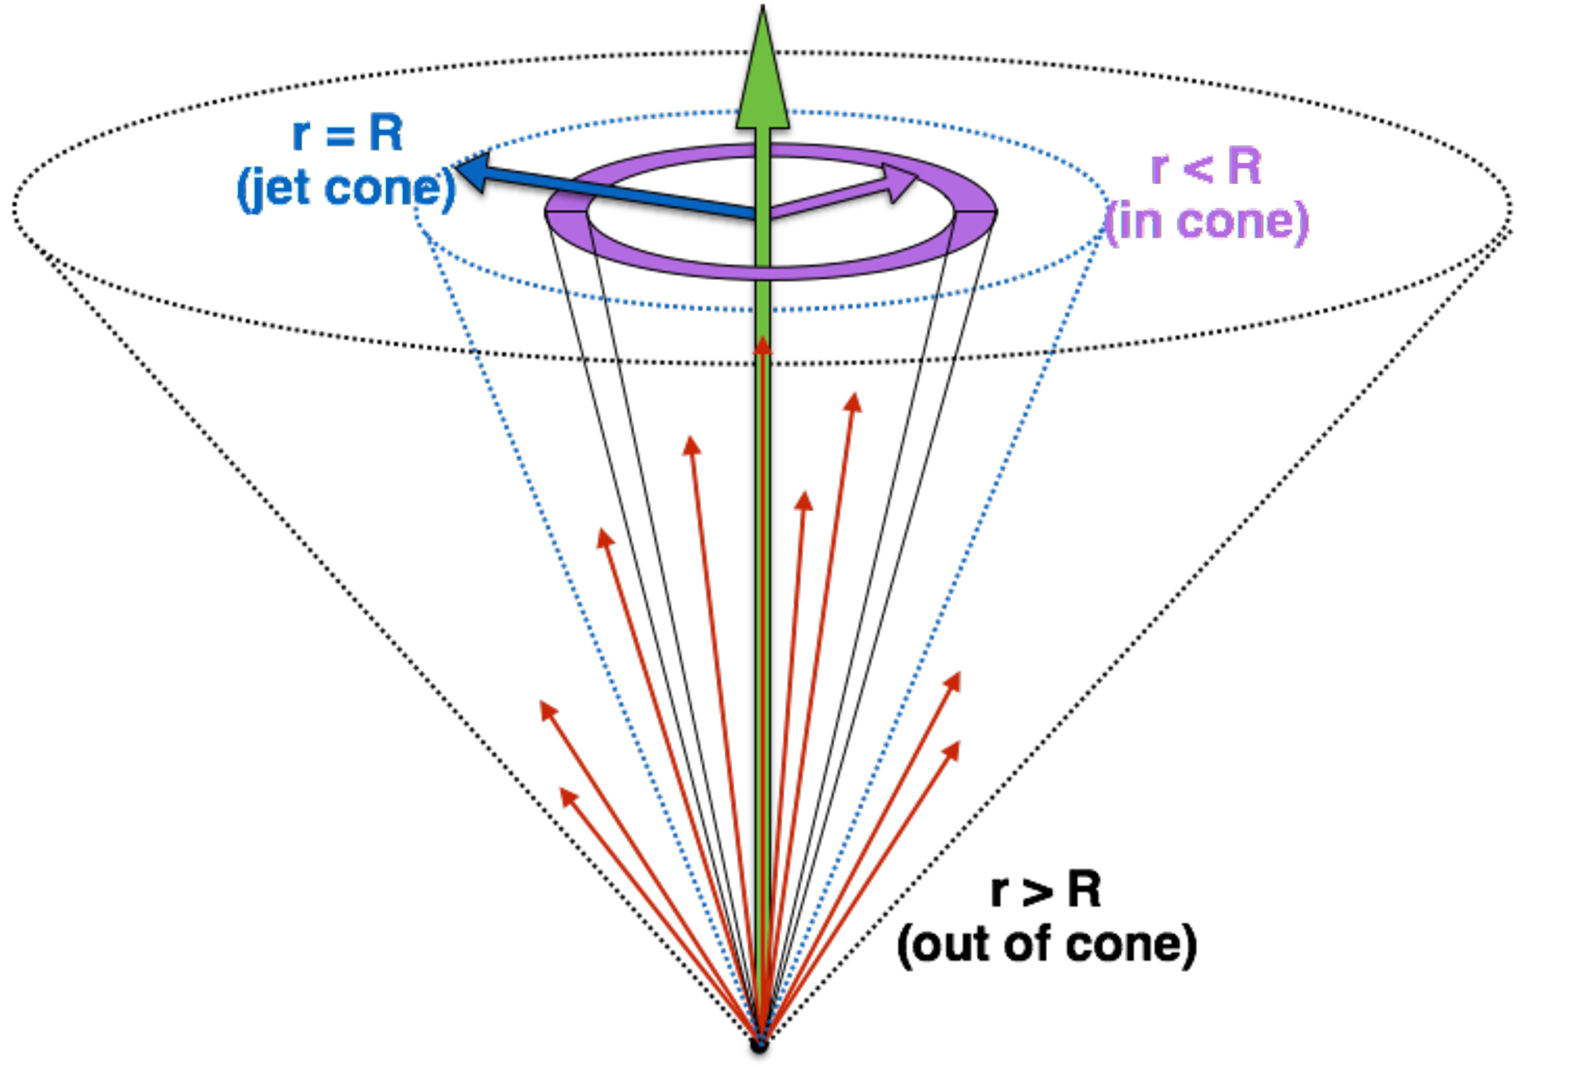
\includegraphics[width=0.55\textwidth]{figures/main/figures_general/fragScheme_Shape.pdf} }
\caption{Illustration of the tracks in and around the jet. }
\label{Fig:dpt_def}
\end{figure}

%These distributions are of interest because they indicate how the energy of the jet is lost both in and outside the jet in \pbpb\ collisions. Similar measurements have been made by CMS~\cite{CMSPASHIN16020, Chatrchyan:2014ava}, and ATLAS~\cite{PhysRevC.98.024908, Aaboud:2017bzv}.

The entire analysis flow of this measurement, along with the various cuts and corrections (discussed in Sec.~\ref{sec:cuts_corrections}) is shown in Fig:\ref{Fig:analysis_flow} and briefly described in the following paragraph.

\begin{figure}
\centerline{
\includegraphics[width=20.cm]{figures/main/figures_general/Shape_analyses_flow.pdf}
}
\caption{The diagram presents various corrections and cuts that are applied during the analysis.}
\label{Fig:analysis_flow}
\end{figure}

First, the measured charged particle yield, $\text{d}n^{\text{meas}}_{\text{ch}}/\text{d}\pTch$, within an annulus with radii $r_{\text{min}}$ and $r_{\text{max}}$ is evaluated as:
\begin{equation}
\frac{\text{d}n^{\text{meas}}_{\text{ch}}}{\text{d}\pTch} = \frac{1}{\epsilon(\pttrk, \etatrk)} \frac{\Delta N_{\text{ch}} (\pTch, r)}{\Delta \pTch}
\end{equation}

where $\Delta N_{\text{ch}} (\pTch, r)$ is the number of charged particles in a given \pTch\ range that passed the jet and track selection criteria, $r = (r_{\text{min}} + r_{\text{max}}) / 2$, and $\epsilon(\pttrk, \etatrk)$ is the charged particles reconstruction efficiency correction, applied on a track-by-track basis. In \pbpb\ collisions, the measured distributions are affected by charged particles from the underlying event, and thus need to be subtracted out (see Sec.~\ref{sec:cuts_corrections} for details):

\begin{equation}
\frac{\text{d}n^{\text{sub}}_{\text{ch}}}{\text{d}\pTch} = \frac{\text{d}n^{\text{meas}}_{\text{ch}}}{\text{d}\pTch} - \frac{\text{d}n^{\text{UE}}_{\text{ch}}}{\text{d}\pTch}
\end{equation}

The final \Dptr\ distributions are then evaluated after unfolding and normalizing with respect to the unfolded number of jets, $N_{\text{jet}}^{\text{unfolded}}$, as well as the area $A$ of the annulus at given distance $r$ :
\begin{equation}
\Dptr = \frac{1}{N_{\text{jet}}^{\text{unfolded}}} \frac{1}{\text{A}} \frac{\text{d}n^{\text{unfolded}}_{\text{ch}}}{\text{d}\pTch} \quad \quad \text{where } A = \pi (r_{\text{max}}^2 - r_{\text{min}}^2)
\end{equation}

The unfolding procedure is a combination of a two-dimensional Bayesian unfolding method in \ptjet\ and \pttrk, one-dimensional Bayesian unfolding method to correct jet spectra for the normalization and a one-dimensional bin-by-bin correction for the jet and track position resolution. 

The analysis is performed differentially in \ptjet, and centrality, with the jet \pt\ bin size growing logarithmically with \ptjet\ to ensure good statistics in the full range of the measurement. This scheme was also used in other ATLAS jet measurements~\cite{ATLAS276FFConf}. 

In order to quantify the differences between charged particle spectra in \pbpb\ and \pp\  collisions, the ratios of the charged particle spectra in \pbpb\ collisions to those in \pp\ collisions are also reported:
\begin{equation}
   R_{\Dptr} \equiv \frac{\Dptr_{\pbpb}}{\Dptr{\pp}}
\end{equation}




\section{Input Data}
\label{sec:used_data}
% !TEX encoding = UTF-8 Unicode
% !TEX root = thesis-ex.tex

\subsection{Data samples}
%\label{sec:data}

This analysis used the original processing of \pp\ (reconstruction tag 7744) and \PbPb\ (reconstruction tag 7874) collisions at \sqrtsnn~=~5.02~TeV recorded in 2015 with a total integrated luminosity of 25 pb$^{-1}$ and 0.49~nb$^{-1}$ respectively.
The run numbers for each set are given below:
\begin{itemize}
\item 2015 \pp\ data: 286282, 286361, 286364, 286367, 286411, 286474
\item 2015 \PbPb\ data: 286711, 286717, 286748, 286767, 286834, 286854, 286908, 286990, 287038, 287044, 287068, 287222, 287224, 287259, 287270, 287281, 287321, 287330, 287334, 287378, 287380, 287382, 287560, 287594, 287632, 287706, 287728, 287827, 287843, 287866, 287924, 287931
\end{itemize}


Various hard probe triggers (high-\pT\ jets, muons, electrons, and photons) are group into a Hard Probe (HP) stream and Main stream in \PbPb\ and \pp\ data taking periods respectively.
The \pp\ data samples from the Main stream used in this analysis are listed in Table~\ref{tab:events}.
For the analysis of the \pbpb\ data the officially produced HION7 derivation samples from the Hard Probe stream are used.
The list of datasets together with detailed description of HION7 derivation setup can be found in Ref.~\cite{HIdataderviation}.
Additionally to the jet triggered data sample, \PbPb\ collisions recorded by Minimum-Bias (MB) triggers grouped in to MB stream are utilized in this analysis.
The following MB data sets are used: \texttt{data15\_hi.0028*.physics\_MinBias\\.merge.AOD.r7874\_p2580}.



\begin{table}[h]
\begin{center}
\begin{tabular}{|c|c|c|}
\hline
description & data set names & \# runs \\ \hline
%\pp, MB &  {\tt \footnotesize data13\_2p76TeV.00219*.physics\_MinBias.merge.NTUP\_HI.f519\_m1313} & 6 \\
%2013 \pp, hard probes &  {\tt \footnotesize data13\_2p76TeV.00219*.physics\_HardProbes.merge.NTUP\_HI.f519\_m1313} 
	    & & 6 \\ \hline
2015 \pp, hard probes &  {\tt \footnotesize data15\_5TeV.periodK.physics\_Main.PhysCont.AOD.repro20\_v03} 
& 5 \\ \hline
2015 \pp, hard probes &  {\tt \footnotesize data15\_5TeV.periodVdM.physics\_Main.PhysCont.AOD.repro20\_v03} 
& 1 \\ \hline
\end{tabular}
\caption{Summary of data samples used in the \pp\ analysis.}
\label{tab:events}
\end{center}
\end{table}

\subsection{Trigger Selection}

%The data used in this study utilize the jet triggered data samples grouped into Hard Probe (HP) stream.


To maintain efficiency for events containing hard probes specific jet triggers are used.
First, events are identified at the L1 trigger by various L1 triggers.
These L1 ``seeds'' are passed to the High Level Trigger (HLT) where jet trigger algorithm with various thresholds on \pT\ of the jet was used for the final selection.


Low \pT\ HLT jet triggers in \pp\ collisions were seeded by L1 MB random trigger ($\texttt{L1RD0}$) or L1 triggers requiring different thresholds on total energy in the calorimeter ($\texttt{L1TE}$).
High \pT\ HLT jet triggers in \pp\ collisions were seeded by different L1 jet triggers performing a simple sliding window algorithm to find jet candidates ($\texttt{L1J}$).
In \PbPb\ collisions, L1 total energy triggers were used to seed all HLT jet trigger chains.

We analyze jets selected from jet triggers in the region of jet \pt\ for which the triggers are fully efficient\footnote{Efficiency is better than 99\%} for jets.
Since the analysis only used jets above 100 GeV, the appropriate triggers were selected.
For \pp, only the {\footnotesize{HLT\_j85}} trigger (fully efficient above 88.8 GeV) was used.
For \pbpb\, the only trigger used was the {\footnotesize{HLT\_j75\_ion\_L1TE50}} (fully efficient above 91 GeV).
   
The performance of the jet trigger in 2015 is described in~\cite{HITMF} and the trigger efficiency is presented in Figure~\ref{fig:Trigger_pp5} (\pp\ collisions) and Figure~\ref{fig:Trigger_PbPb} (\pbpb\ collisions).
The trigger efficiency for two low thresholds is evaluated using MB events.
The low \pT\ thresholds are used as the reference to evaluate the performance at higher \pT.
The efficiency for the higher threshold is bootstraped from lower thresholds.
The broader turn-on of the jet trigger in \pbpb\ compared to \pp\ collisions is caused by significant differences between the HI jet trigger reconstruction algorithm used at the time of the data taking and the current version of the offline reconstruction software.

  \begin{figure}[h]
 \centerline{
 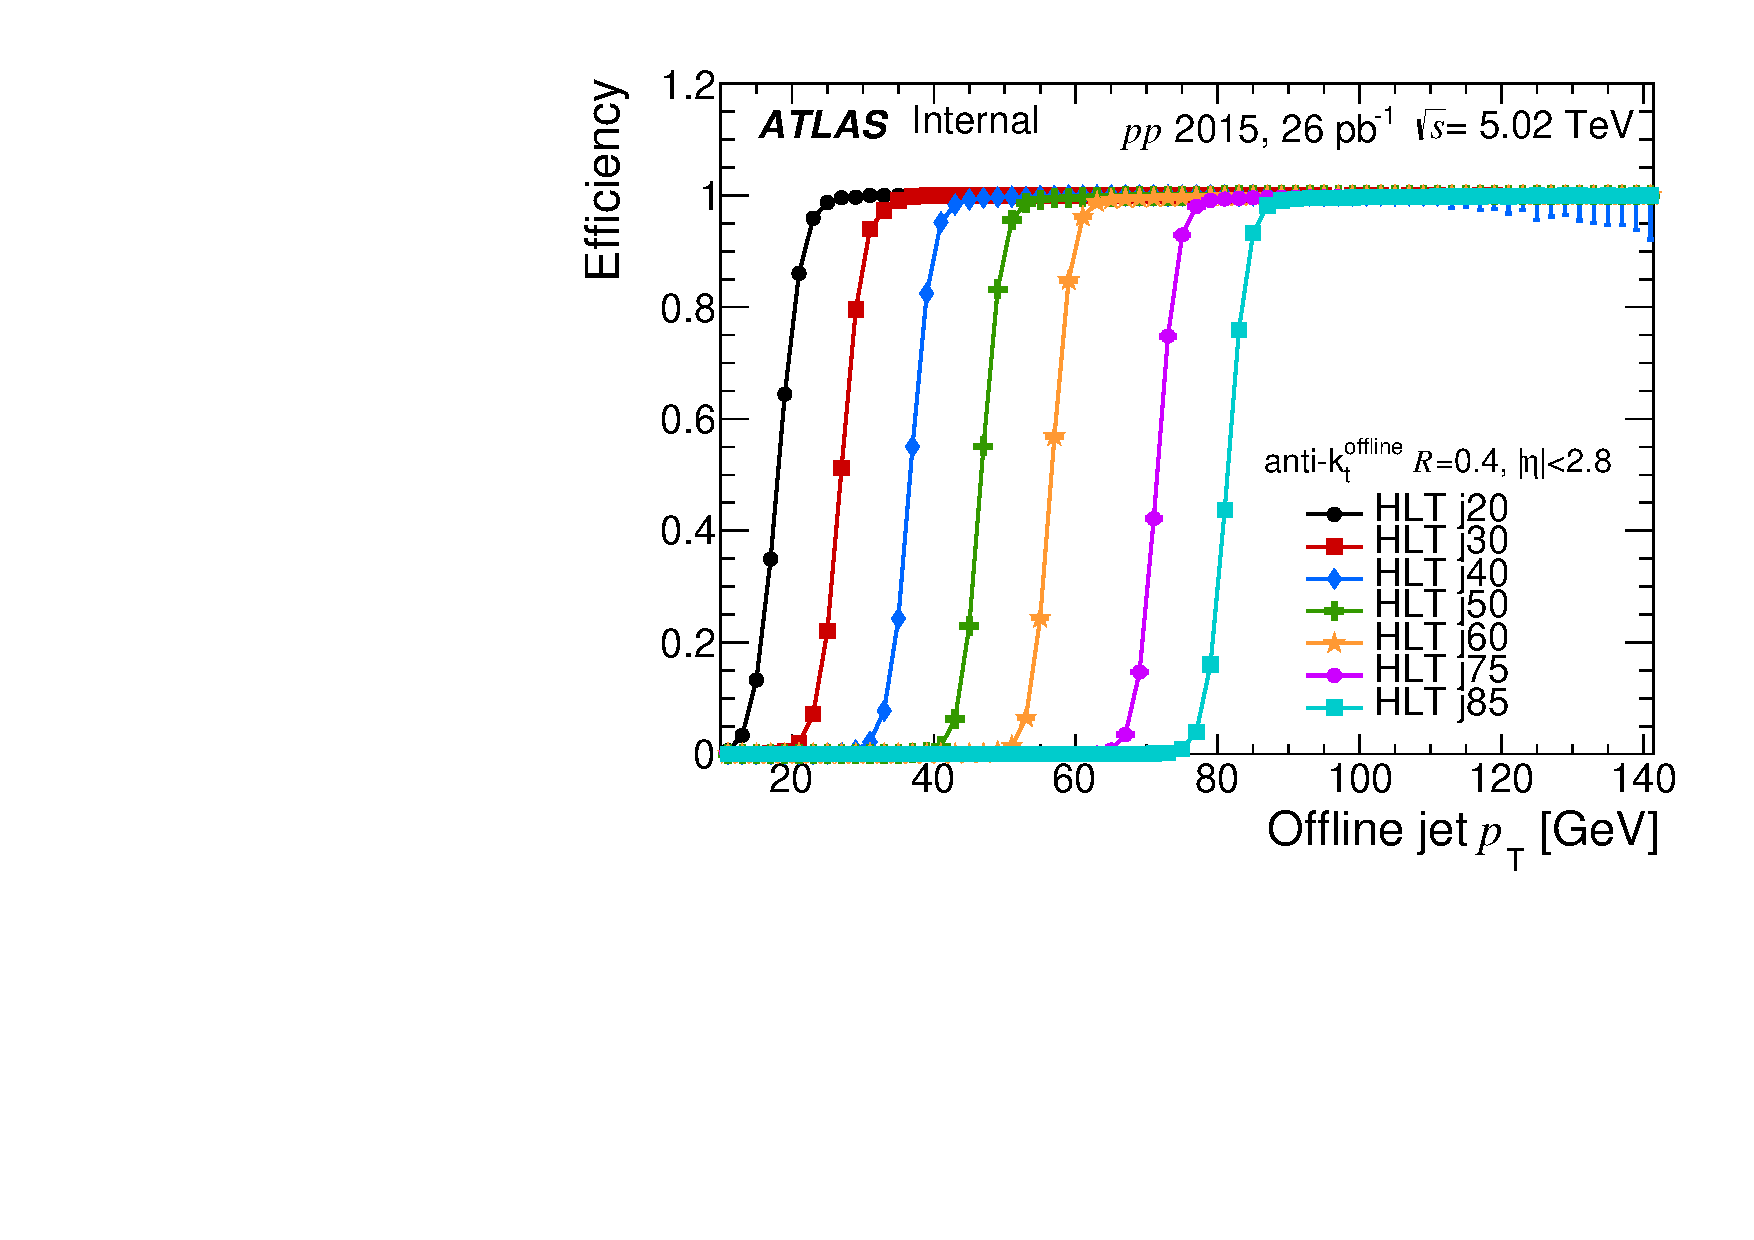
\includegraphics[width=0.75\textwidth]{figures/main/general/Eff_pp_5TeV_central.pdf}
}
 \caption{Trigger efficiencies for R=0.4 offline jets for seven HLT jet triggers in \pp\ collisions at 5.02 TeV.}
\label{fig:Trigger_pp5}
 \end{figure}


 \begin{figure}[h]
    \centerline{
       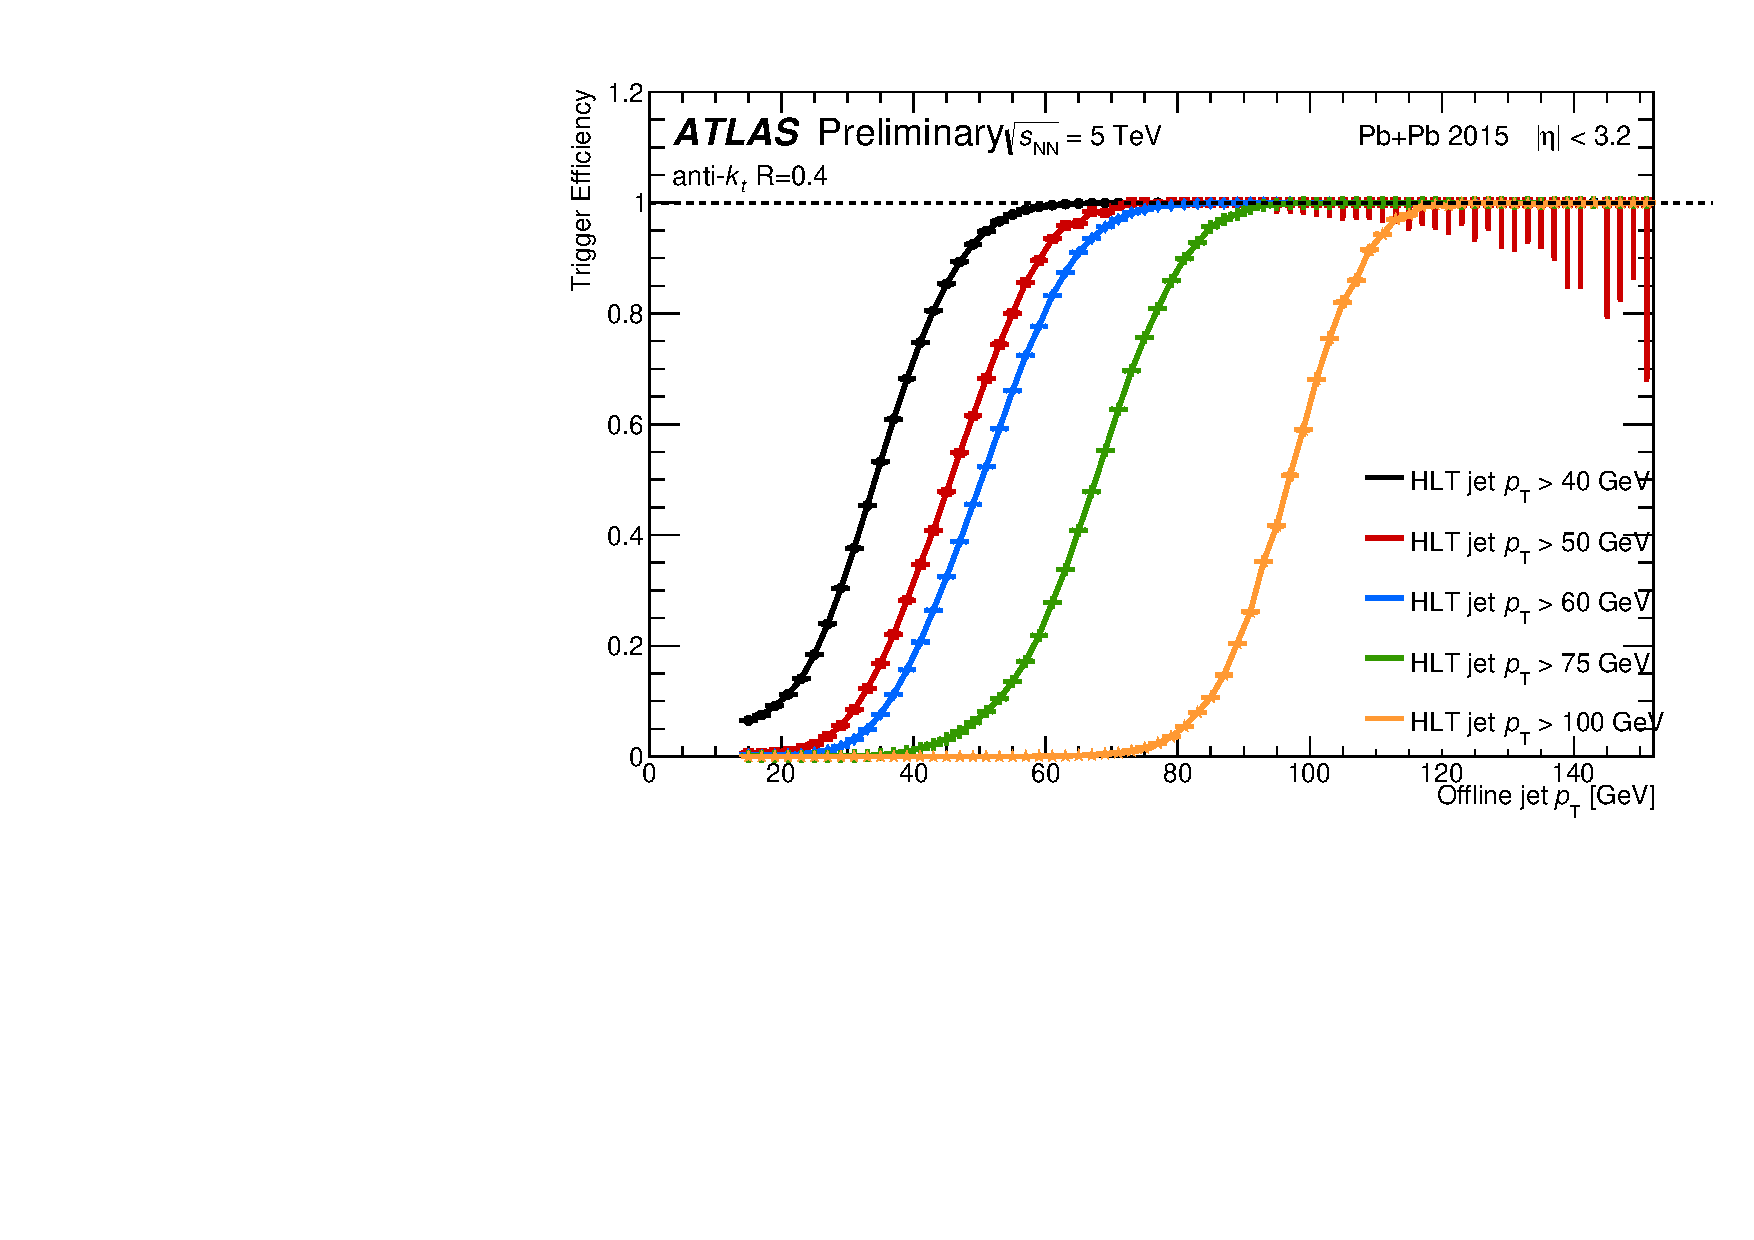
\includegraphics[width=0.75\textwidth]{figures/main/general/trigger_eff_PbPb_CentInclusive.pdf}
    }
    \caption{Jet trigger efficiency in centrality inclusive (0-80\%) \pbpb\ collisions for R=0.4 offline
    jets.}
    \label{fig:Trigger_PbPb}
 \end{figure}

In addition to the jet triggered sample, a MB triggered sample defined by a logical OR of the total energy trigger with a threshold of 50~\GeV\ and the ZDC coincidence trigger was used as part of the MC overlay procedure

The event fraction as a function of run number for both the hard probes stream and the minimum bias overlay stream in \pbpb\ is shown in Figure~\ref{fig:evnt_fraction}

 \begin{figure}[h]
    \centerline{
       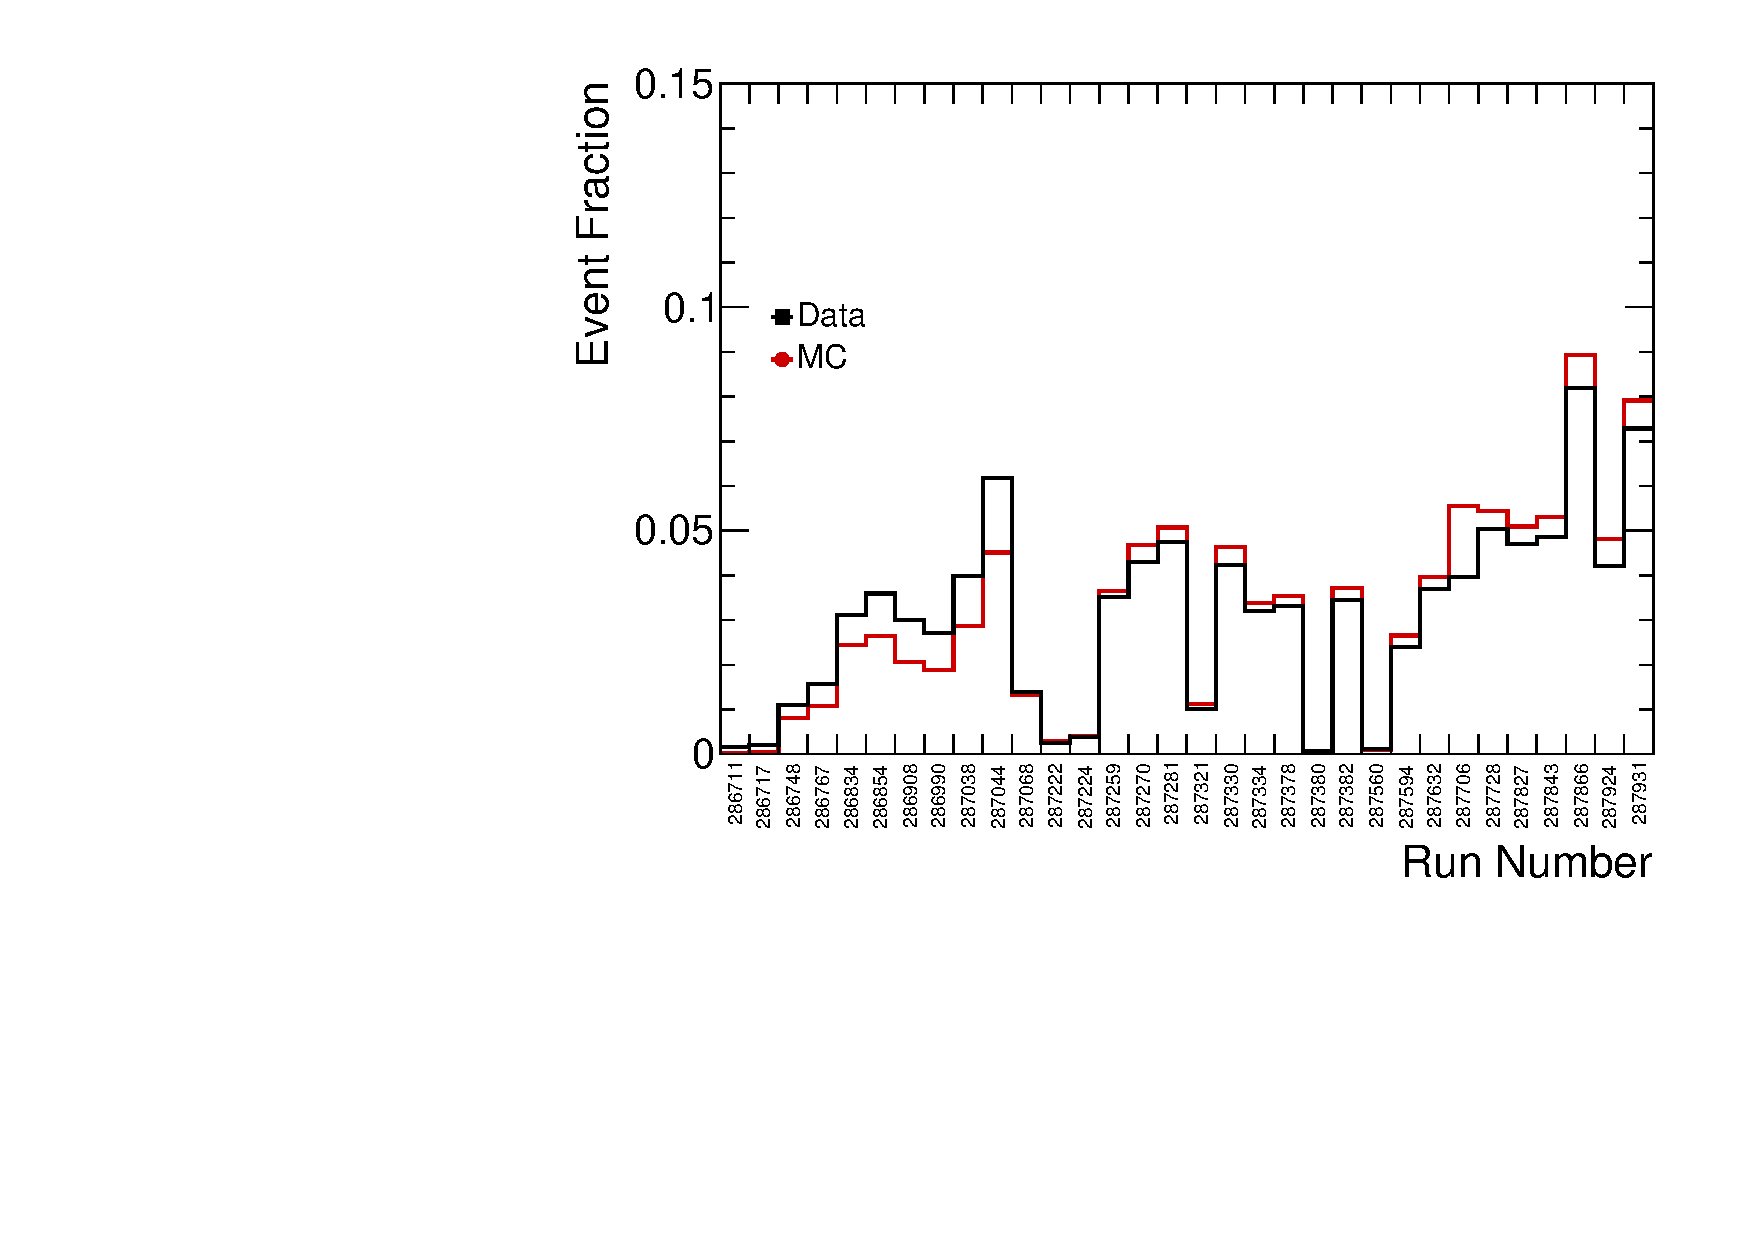
\includegraphics[width=0.9\textwidth]{figures/main/general/EventPercentages_c0.pdf}
    }
    \caption{Event fraction as a function of runs for Hard Probes and the Minimum Bias Overlay Streams in \pbpb\ collisions.}
    \label{fig:evnt_fraction}
 \end{figure}

The run dependence of the underlying event (a core part of this measurement) was tested by dividing the data and MC into three periods with approximately equal number of events in each period: 286711 -- 287259, 287270 -- 287632, and 287706 -- 287931.
The underlying event determined for each period compared to the nominal underlying event evaluated for the entire dataset is shown in Figure~\ref{fig:weighted_runs}, and it can be seen that the UE is stable throughout the data taking period.
%The systematic uncertainty associated with the run dependence was included in the calculation of the systematic uncertainty on the result.

 \begin{figure}[h]
    \centerline{
       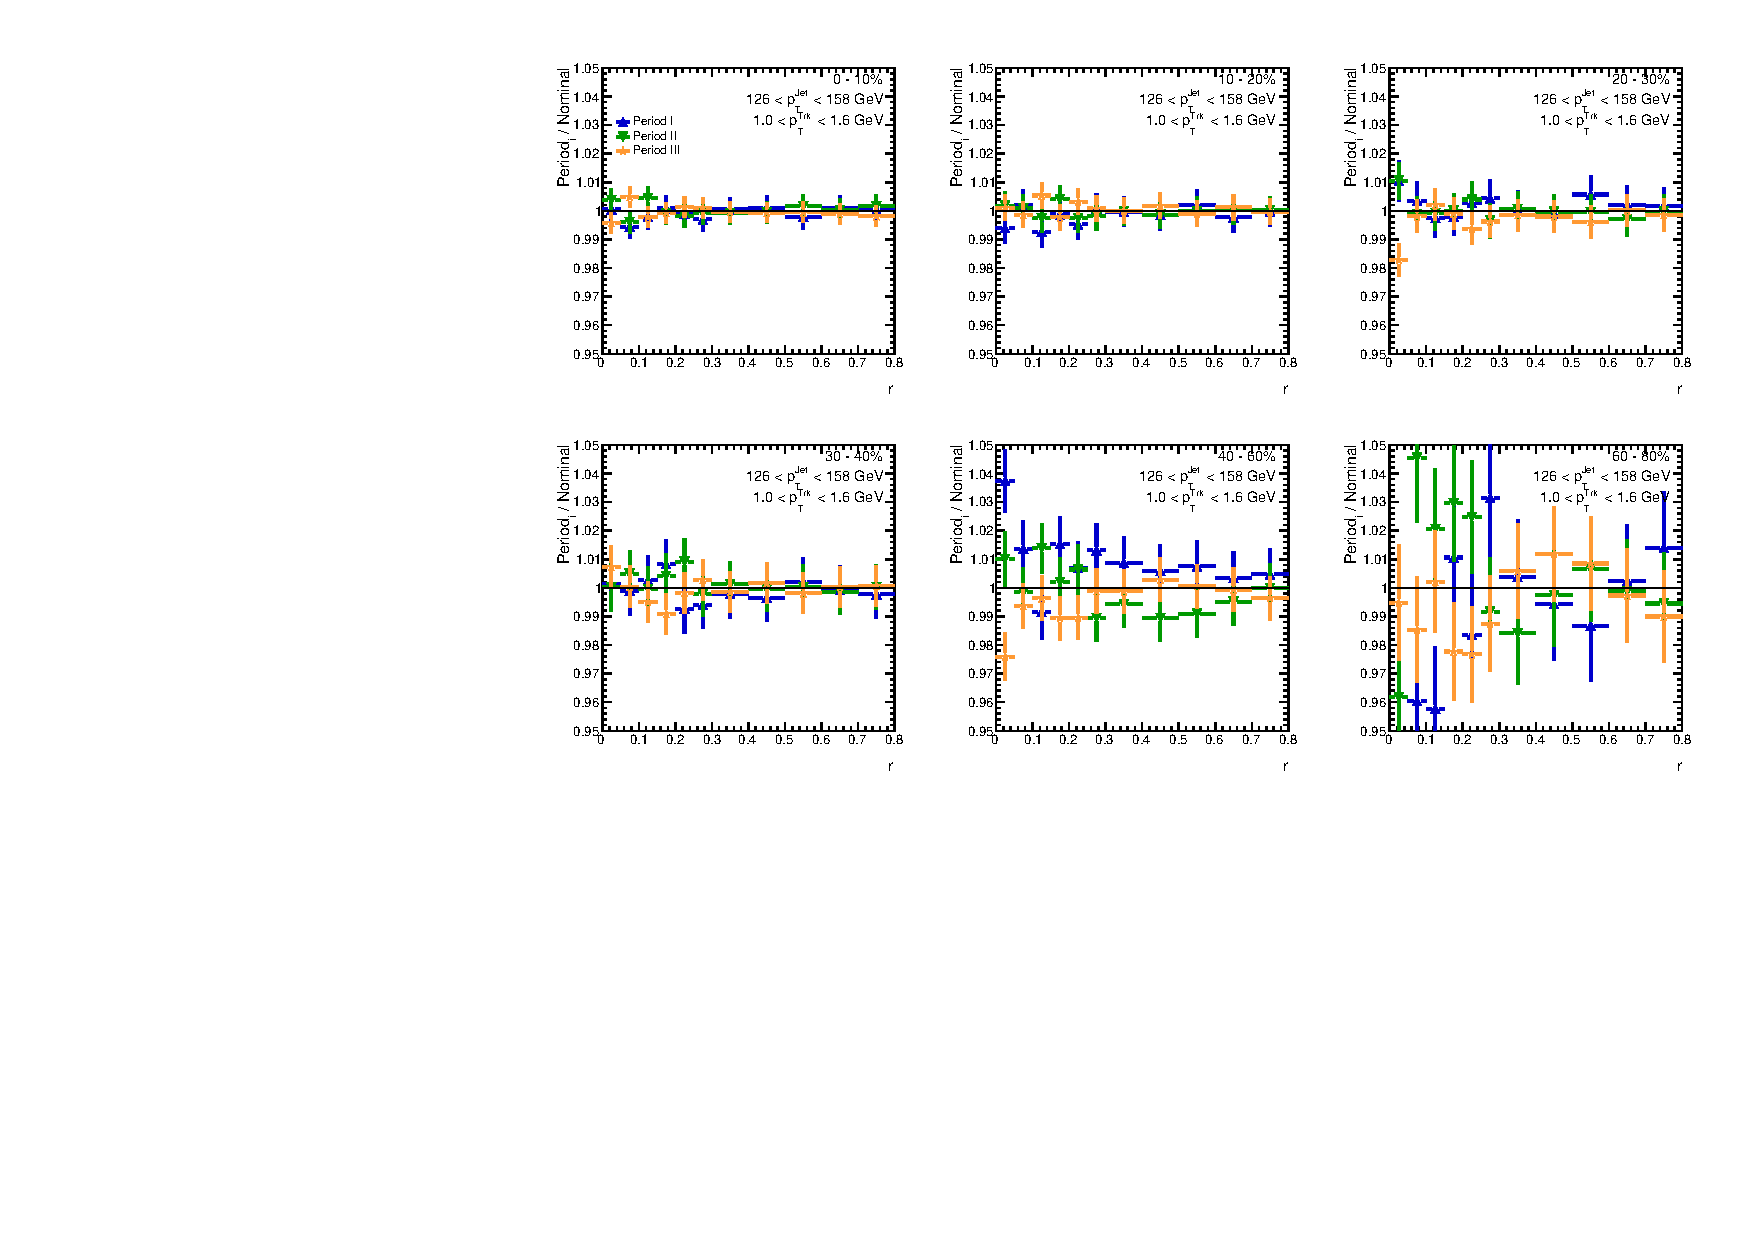
\includegraphics[width=0.75\textwidth]{figures/main/general/weightedRuns.pdf}
    }
    \caption{Stability of the underlying event for three different periods of the data taking.
The different curves indicate the ratio of the underlying event in each period of data taking to the underlying event determined in the entire dataset.}
    \label{fig:weighted_runs}
 \end{figure}


%%%%%%%%%%%%%%%%%%%%%%%%%%
% two separate MB data sample are used: 1) to estimate the underlying event contribution of charged particles to measured distributions; 2) to study detector performance in conditions that match the data.
The first sample was recorded by MB triggers requiring either to have the transverse energy in the whole calorimeter exceeding 50 GeV at the Level-1 trigger (HLT\_noalg\_mb\_L1TE50) or to have a track reconstructed in the inner detector in coincidence with ZDC signals on both sides (HLT\_mb\_sptrk\_ion\_L1ZDC\_A\_C\_VTE50).
The second sample was recorded with the MB trigger defined by a logical OR of the total energy trigger with a threshold of 50~\GeV\ and the ZDC coincidence trigger.
This sample was used because it was utilized in the MC overlay procedure.
Furthermore, two total transverse-energy triggers requiring 1.5~\TeV\ and 6.5~\TeV\ were used to enhance higher multiplicity events.

%
%   \begin{table}[h]
%\centering
%\begin{tabular}{|c|c|}
%\hline
%trigger & \ptjet (GeV) \\
%\hline
%%{\tt \footnotesize EF\_j20} & 25.7-35.2\\
%%{\tt \footnotesize EF\_j30\_L1TE5} & 35.2-43.6\\
%%{\tt \footnotesize EF\_j40\_L1TE5}  & 43.6-52.8\\
%%{\tt \footnotesize EF\_j50\_L1J12} & 52.8-62.5\\
%%{\tt \footnotesize EF\_j60\_L1J15} & 62.5-78.8\\
%%{\tt \footnotesize EF\_j75\_L1J20} & 78.8-88.8\\
%{\tt \footnotesize EF\_j85} & $>$~88.8\\
%\hline
%\end{tabular}
%\caption{Triggers used in the analysis of 2015 \pp\ data and the corresponding \ptjet\ ranges.}
%\label{tab:jettrigpp5}
%\end{table}
%
%\begin{table}
%\centering
%\begin{tabular}{|c|c|}
%\hline
%trigger & \ptjet (GeV) \\
%\hline
%{\tt \footnotesize EF\_j75\_ion\_L1TE50} & $>$~91\\
%%{\tt \footnotesize EF\_j100\_ion\_LITE50} & $>$~114\\
%\hline
%\end{tabular}
%\caption{Triggers used in the analysis of 2015 \pbpb\ data and the corresponding \ptjet\ ranges.}
%\label{tab:jettrigpbpb5}
%\end{table}



%The studies in this note utilize high-statistic MC samples that are used to study the performance of the analyses and in the unfolding procedure.
%The MC12 PYTHIA6.4 \pp\ di-jet events at $\sqrt{s} =5.02$~TeV with the same rapidity shift in the center of mass as in the data, were embedded on top of heavy ion MB data events collected during the 2013 run using a MB trigger in \texttt{MinBiasOverlay} stream.
%The \texttt{MinBiasOverlay} records the data without zero suppression.
%The signal from this trigger was combined with the signal from PYTHIA6.4 at the digitization stage and then reconstructed as a combined event.
%MC samples are used for both the period A and period B running conditions.
%Truth jets with \pTtrue\ were defined in the MC sample as the output of the \antikt\ algorithm with \RFour\ applied to the final-state particles generated by PYTHIA6.4.
%%%%%%%%%%%%%%%%%%%%%%%%%%%%%%

\subsection{Monte Carlo Samples}

 

This analysis also utilizes MC15 \pythiaeight\ \pp\ jet events at $\sqrt{s} =5.02$~TeV with the A14 ATLAS tune and the NNPDF23LO pdfs~\cite{ATLAS2014021}.
The definitions of the \pp\ MC samples can be found in Tab.~\ref{Tab:MCSamples_pp5}.
The \pbpb\ MC uses POWHEG+\pythiaeight\ events that are overlayed on top of MB \PbPb\ collisions.
 
These samples are listed in Tab.~\ref{tab:overlay}.


\begin{table}[htbp]
\centering
\begin{tabular}{|l|p{0.65\linewidth}|}
\hline
\multicolumn{1}{|c|}{JZ} & \multicolumn{1}{c|}{Dataset Name}                 		                                  \tabularnewline \hline
2	& {\tt \footnotesize mc15\_5TeV.420022.PowhegPythia8EvtGen\_A14\_NNPDF23LO\_CT10ME\_ jetjet\_JZ2R04.merge.DAOD\_HION7.e4109\_s2860\_r7792\_r7676\_p3442}                                                     \tabularnewline \hline
3	& {\tt \footnotesize mc15\_5TeV.420023.PowhegPythia8EvtGen\_A14\_NNPDF23LO\_CT10ME\_ jetjet\_JZ3R04.merge.DAOD\_HION7.e5067\_s2860\_r7792\_r7676\_p3442}                                                                                  \tabularnewline \hline
4	& {\tt \footnotesize mc15\_5TeV.420024.PowhegPythia8EvtGen\_A14\_NNPDF23LO\_CT10ME\_ jetjet\_JZ4R04.merge.DAOD\_HION7.e5067\_s2860\_r7792\_r7676\_p3442}                                                                   \tabularnewline \hline
\end{tabular}
\begin{tabular}{| c | c | c | c | c |} \hline
J & \RFour\ \pTtrue\ [\GeV]  & $\sigma$ [$\mathrm{nb}$] $\times$ $\epsilon$ & $\#$events \\ \hline
2  & 60--160 &  (6.4 $\times$ 10$^5$) $\times$ (4.27 $\times$ 10$^{-3}$) & 5.8 M \\ \hline
3  & 160--400 &  (4.7 $\times$ 10$^3$) $\times$ (5.28 $\times$ 10$^{-3}$) & 5.9 M \\ \hline
4  & 400--800 &  (2.7 $\times$ 10$^1$)  $\times$ (4.58 $\times$ 10$^{-3}$) & 5.8 M \\ \hline
\end{tabular}
\caption{5.02 TeV \pythiaeight\ \pp\ MC samples.}
\label{Tab:MCSamples_pp5}
\end{table}


\begin{table}[htbp]
\centering
\begin{tabular}{|l|p{0.65\linewidth}|}
\hline
\multicolumn{1}{|c|}{JZ} & \multicolumn{1}{c|}{Dataset Name}                 		                                  \tabularnewline \hline
2	& {\tt \footnotesize mc15\_5TeV.420022.PowhegPythia8EvtGen\_A14\_NNPDF23LO\_CT10ME\_jetjet \_JZ2R04.merge.DAOD\_HION7.e4109\_d1421\_r8238\_r8052\_p3196}                                                     \tabularnewline \hline
3	& {\tt \footnotesize mc15\_5TeV.420023.PowhegPythia8EvtGen\_A14\_NNPDF23LO\_CT10ME\_jetjet \_JZ3R04.merge.DAOD\_HION7.e4109\_d1421\_r8238\_r8052\_p3196}                                                                                  \tabularnewline \hline
4	& {\tt \footnotesize mc15\_5TeV.420024.PowhegPythia8EvtGen\_A14\_NNPDF23LO\_CT10ME\_jetjet \_JZ4R04.merge.DAOD\_HION7.e4109\_d1421\_r8238\_r8052\_p3196}                                                                   \tabularnewline \hline
\end{tabular}
\caption{\pbpb\ data overlay datasets used here.}
\label{tab:overlay}
\end{table}



\section{Event Selection }
\label{sec:event_selection}
% !TEX root = thesis-ex.tex

The standard ATLAS event quality requirements were applied for the event selection both for the \pp\ and \PbPb\ event selection.
\begin{itemize}
\item All the sub-detector systems were required to be fully functional: all the data were required to pass the official good run list:
 \\ $\texttt{\scriptsize data15\_5TeV.periodAllYear\_DetStatus-v75-repro20-01\_DQDefects-00-02-02\_PHYS\_HeavyIonP\_All\_Good.xml}$ (2015 \pp) 
 \\ $\texttt{\scriptsize data15\_5TeV.periodVdM\_DetStatus-v75-repro20-01\_DQDefects-00-02-02\_PHYS\_HeavyIonP\_All\_Good.xml}$ (2015, VdM \pp)
 \\ $\texttt{\scriptsize data15\_hi.periodAllYear\_DetStatus-v75-repro20-01\_DQDefects-00-02-02\_PHYS\_HeavyIonP\_All\_Good.xml } $ (2015 \pbpb).

\item All events are required to have a good reconstructed primary vertex.
\item The primary vertex must be within 150~mm from the center of ATLAS detector, as a fiducial tracking region.
 
\item Additional event cleaning to remove additional detector imperfections as described here~\cite{2015EventCleaning} is used. 
\item In \PbPb\ collisions the pileup contribution is removed using the  $\texttt{HIAnalysisTools}$ \cite{HIAnalysisTools}. 
\end{itemize}


Figures~\ref{Fig:EventCounts} presents the total number of \pp\ and \pbpb\ events, respectively, entering the analysis together with rejection power of various event quality cuts. A slightly higher fraction of empty events without primary vertex is observed in pp collisions. Some of these events are rejected by multiple cuts. ``Rejection by centrality'' indicates the number of event in HP stream that is outside the 0-80\% centrality bin.

\begin{figure}
\centerline{
\begin{tabular}{cc}
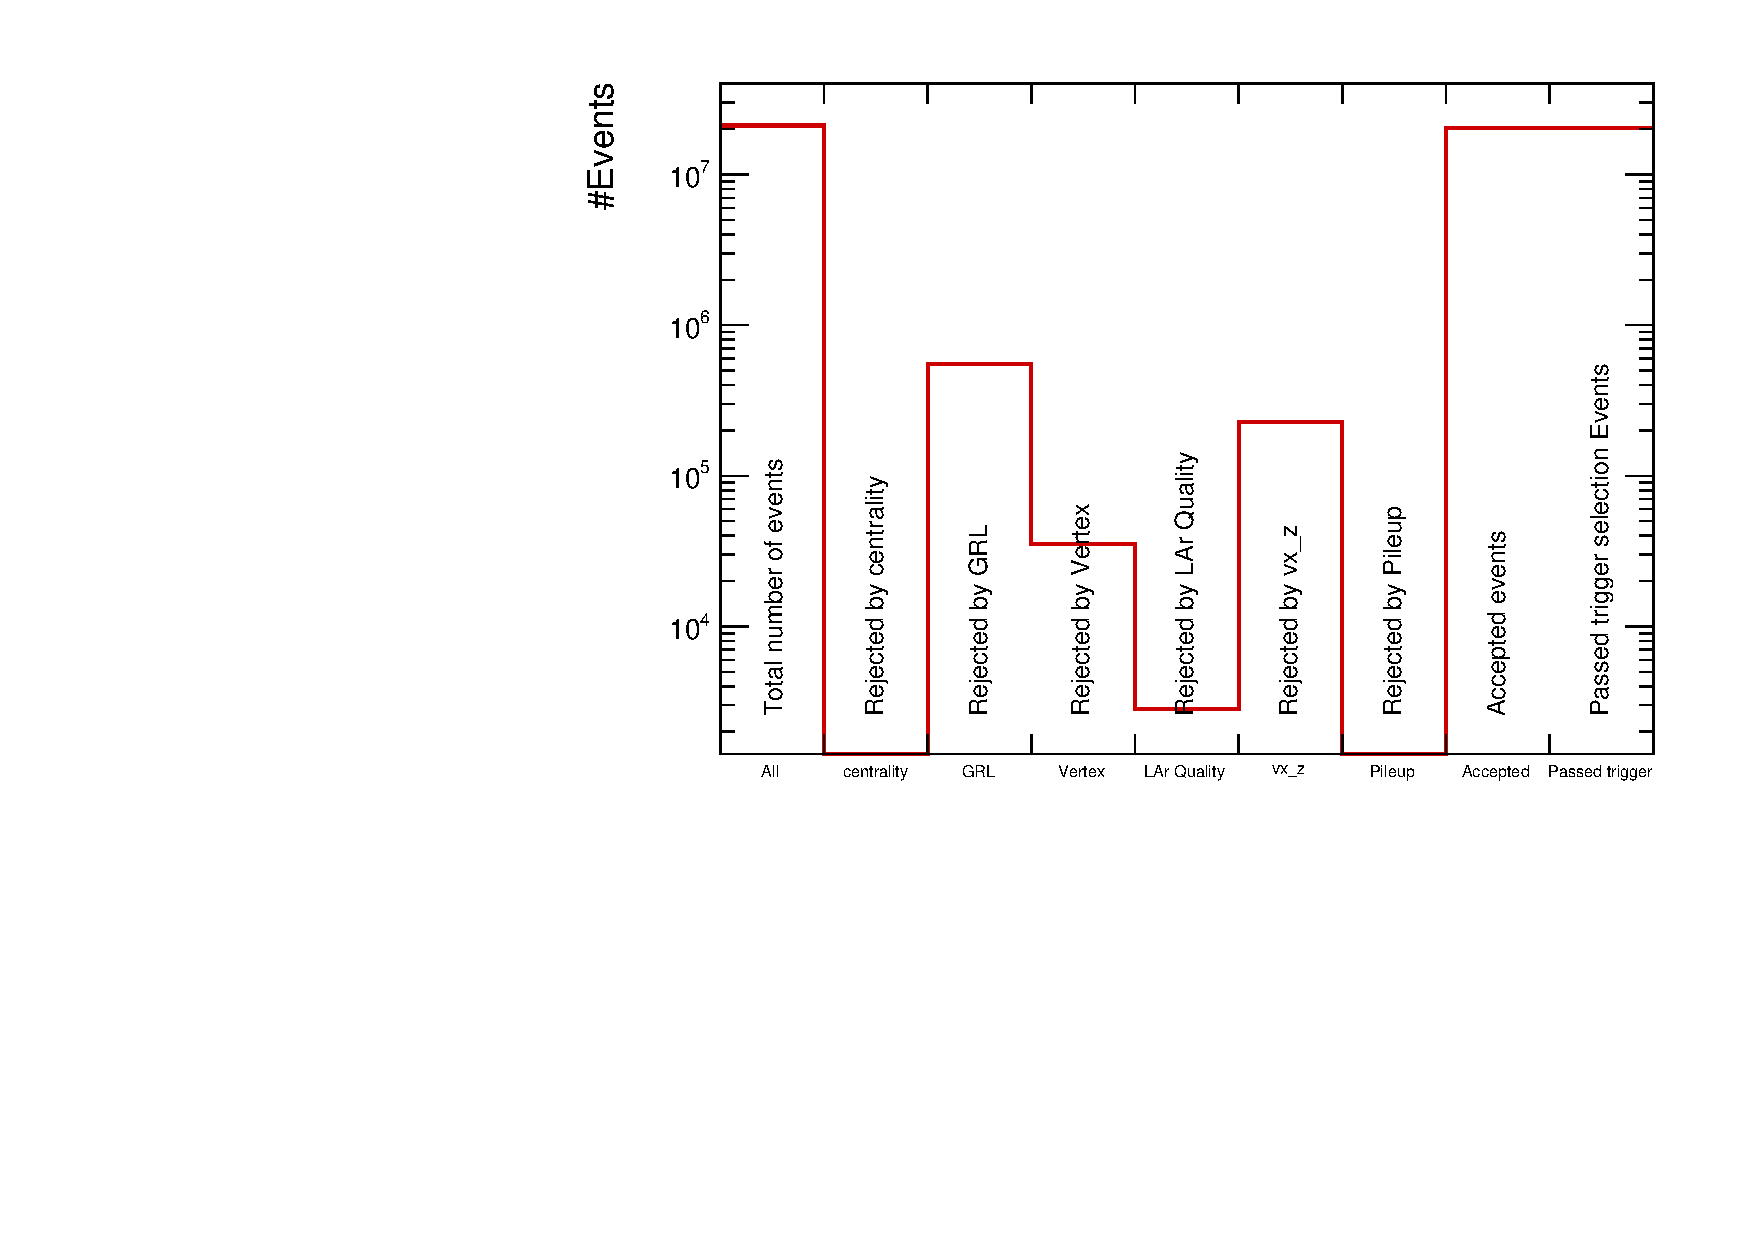
\includegraphics[width=0.45\textwidth]{figures/main/figures_general/EventAccept_pp.pdf} & 
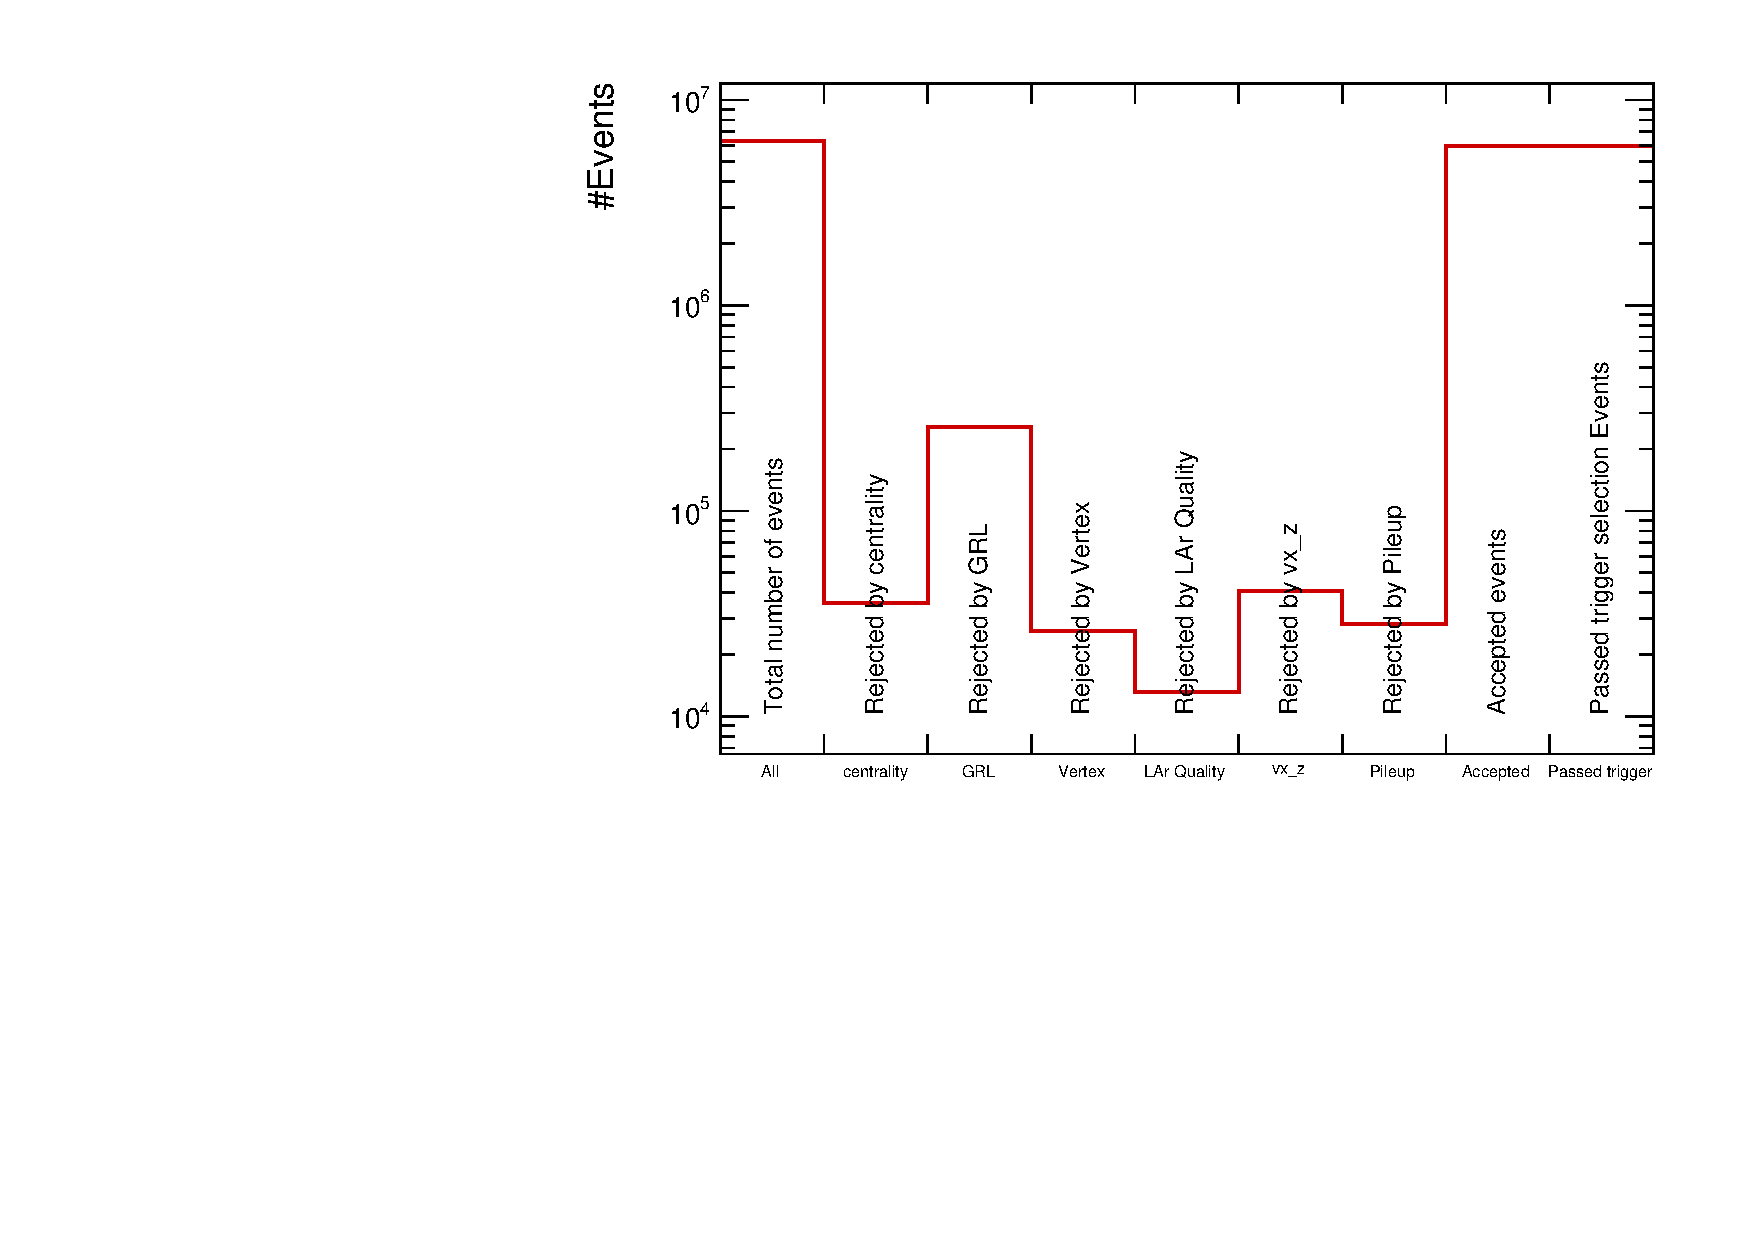
\includegraphics[width=0.45\textwidth]{figures/main/figures_general/EventAccept_PbPb.pdf}
\end{tabular}}
\caption{
The number of 2015 \pp\  (left) and \PbPb\ (right) events used and rejected by various event quality cuts. }
\label{Fig:EventCounts}
\end{figure}


\subsection{Centrality Selection}
\label{sec:cent}

The centrality of the collision is a degree of the overlap of two colliding nuclei that can be quantified by the impact parameter that is the distance between the centers of the two nuclei. If they collide head on the collision is central, if they just graze each other we speak about peripheral collisions. We cannot measure the impact parameter to determine the centrality, but we can measure the overall event activity in the collision, characterized e.g. by the sum of \Et\ measured in FCal calorimeters on both sites. Central collisions have large \Et\ deposits in the FCal, peripheral have small \Et\ deposits.

In this analysis, The \ETfcal\ distribution is divided into percentiles of the total inelastic cross section for \PbPb\ collisions. The first percentile, $0-10\%$, represents the $10\%$ of collisions with the largest event activity, smallest impact parameter. The last percentile, $90-100\%$, represents the $10\%$ of collisions where there is the smallest event activity and largest impact parameter. 
Seven centrality classes have been used: 0-10\%, 10-20\%, 20-30\%, 30-40\%, 40-60\%, 60-80\%. 
The most peripheral collisions 80-100\%, are excluded due to  the small number of jets.
The centrality selections are documented in Ref.~\cite{ref:centrality}. The \PbPb\ MC is re-weighted in the way that it has the same centrality distribution as the jet triggered data sample.

\clearpage


\section{Jet Reconstruction}
\label{sec:reconstruction}
% !TEX encoding = UTF-8 Unicode
% !TEX root = thesis-ex.tex

\label{Sec:JetRec}
For the measurement presented here, we use the jets reconstructed in the calorimeter 
using the \antikt\ algorithm \cite{Cacciari:2008gp} with \RFour.
The underlying event (UE) contribution to jets is subtracted on 
an event by event basis at the cell level. The details on the jet reconstruction 
procedure and performance in heavy ion collisions have been described in 
\cite{ATLAS-COM-PHYS-2011-1733}, here we will only shortly summarize the main 
features of the heavy ion jet reconstruction.

In order to reconstruct jets in heavy ion collisions, a large background from 
the UE has to be subtracted from each jet. 
The UE subtraction procedure is done in several iterative steps. 
First an estimate of the UE average transverse energy density, $\rho_i(\eta)$, 
is evaluated for each calorimeter layer $i$ in intervals of $\eta$ of width 
$\Delta \eta = 0.1$ using all cells in each calorimeter layer, within a given 
$\eta$ interval excluding those within $\Delta R < 0.4$ of ``seed'' jets. In the first 
subtraction step, the ``seed'' jets are defined to be jets reconstructed using the 
\antikt\ algorithm with \RTwo\ jets which have at 
least one tower  (a tower is a 0.1x0.1 region of the calorimeter and the energy
associated with it is the sum of the energies from all contributing calorimeter layers
in that region)
with $\Et > 3$~GeV and which have a ratio of the maximum to 
the mean tower associated with the jet of at least 4. 
  The UE-subtracted cell energies  were calculated according to:
\begin{equation}
\label{eqn:UE}
E_{\mathrm{T},i}(\eta, \phi)^{\mathrm{sub}} = E_{\mathrm{T},i}(\eta, \phi) - A_i \times \rho_i(\eta) 
\end{equation}
where $E_{\mathrm{T},i}$, $\eta$, $\phi$,  and $A_i$ represent the $\Et$, $\eta$, 
$\phi$, and area of the cell in the layer $i$. The $\rho_i(\eta)$ is the energy density per unit area in the layer $i$. The kinematics for \RTwo\ jets 
generated in this first subtraction step were calculated via a four-vector sum 
of all (assumed massless) cells contained within the jets using the \Et\ values 
obtained from Eq.~\ref{eqn:UE}.

The second subtraction step starts with the definition of a new set of 
seeds using a list of \RTwo\ calorimeter jets from the first 
subtraction step, each with $\Et > 4$~GeV. Using this new set of 
seeds, a new estimate of the UE, $\rho'_i(\eta)$, was calculated excluding 
cells within $\Delta R < 0.4$ of the new ``seed'' jets, where $\Delta R = \sqrt{ 
(\eta_{\mathrm{cell}} - \eta_{\mathrm{jet}})^2 + (\phi_{\mathrm{cell}} - \phi_{\mathrm{jet}})^2}$.


The jet energy scale calibration is based on the numerical inversion method and provides calibration constants for all jet collections used in this study~\cite{HICalib}. The final jet energy calibration using in-situ studies is applied in the offline analysis and it is described in Sec~\ref{Sec:JetSelection}.   



The jet reconstruction performance in 5.02 TeV \pp\ collisions was evaluated using corresponding MC samples with a full detector simulation. The kinematics of the truth jets are reconstructed from primary particles\footnote{Primary particles are defined as having a mean lifetime of $\tau > 0.3 \times 10^{-10}$ s, and are produced directly in \pp\ interactions or from decays of particles with shorter lifetimes} with the \antikt\ algorithm with radius parameter $R = 0.4$. The jet reconstruction efficiency, JES (in this case evaluated as $\langle (\ETreco)\rangle/\ETtrue$), and JER for \pp\ collisions is shown in Fig.~\ref{Fig:Performancepp5} for \RFour\ jet.
For \pbpb\ collisions the JES is shown in Fig.~\ref{Fig:PerformancepbpbJES} and the JER is shown
in Figure~\ref{Fig:PerformancepbpbJER}.  Further studies of the jet performance in the 2015 \pbpb\
data are found in Ref.~\cite{Aad:2014bxa}. Figures~\ref{Fig:PerformancepbpbJPReta0p4}-\ref{Fig:PerformancepbpbJPRphi0p4} present the jet angular resolution in $\eta$ and $\phi$ as a function of jet \pt\ evaluated in six centrality classes. The angular resolution is improving with the increasing jet \pT\ and decreasing collision centrality. The angular resolution is found to be significantly better for smaller jets as expected since the smaller jets are less affected by the presence of the UE. 

\begin{figure}
\centerline{
\begin{tabular}{cc}
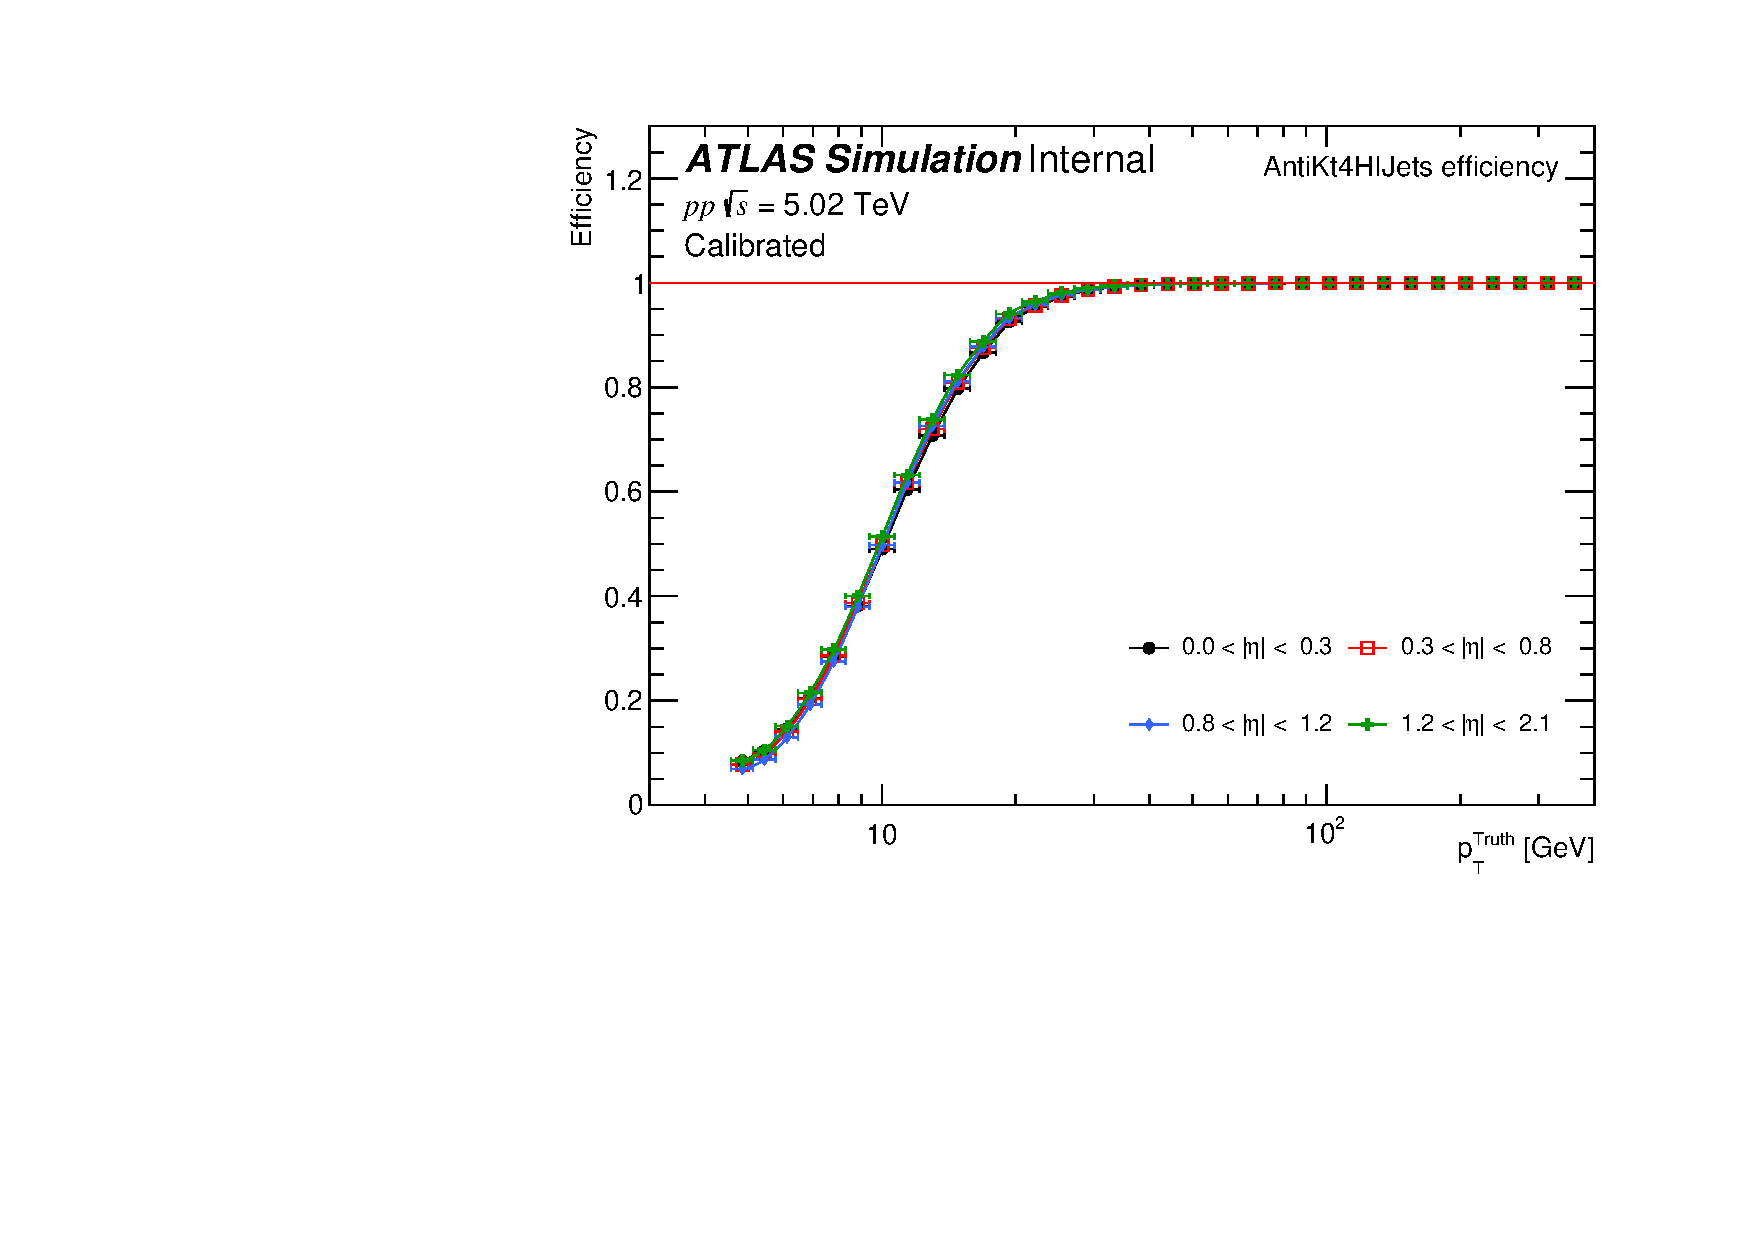
\includegraphics[width=7cm]{figures/main/general/Eff_pp5.pdf} &
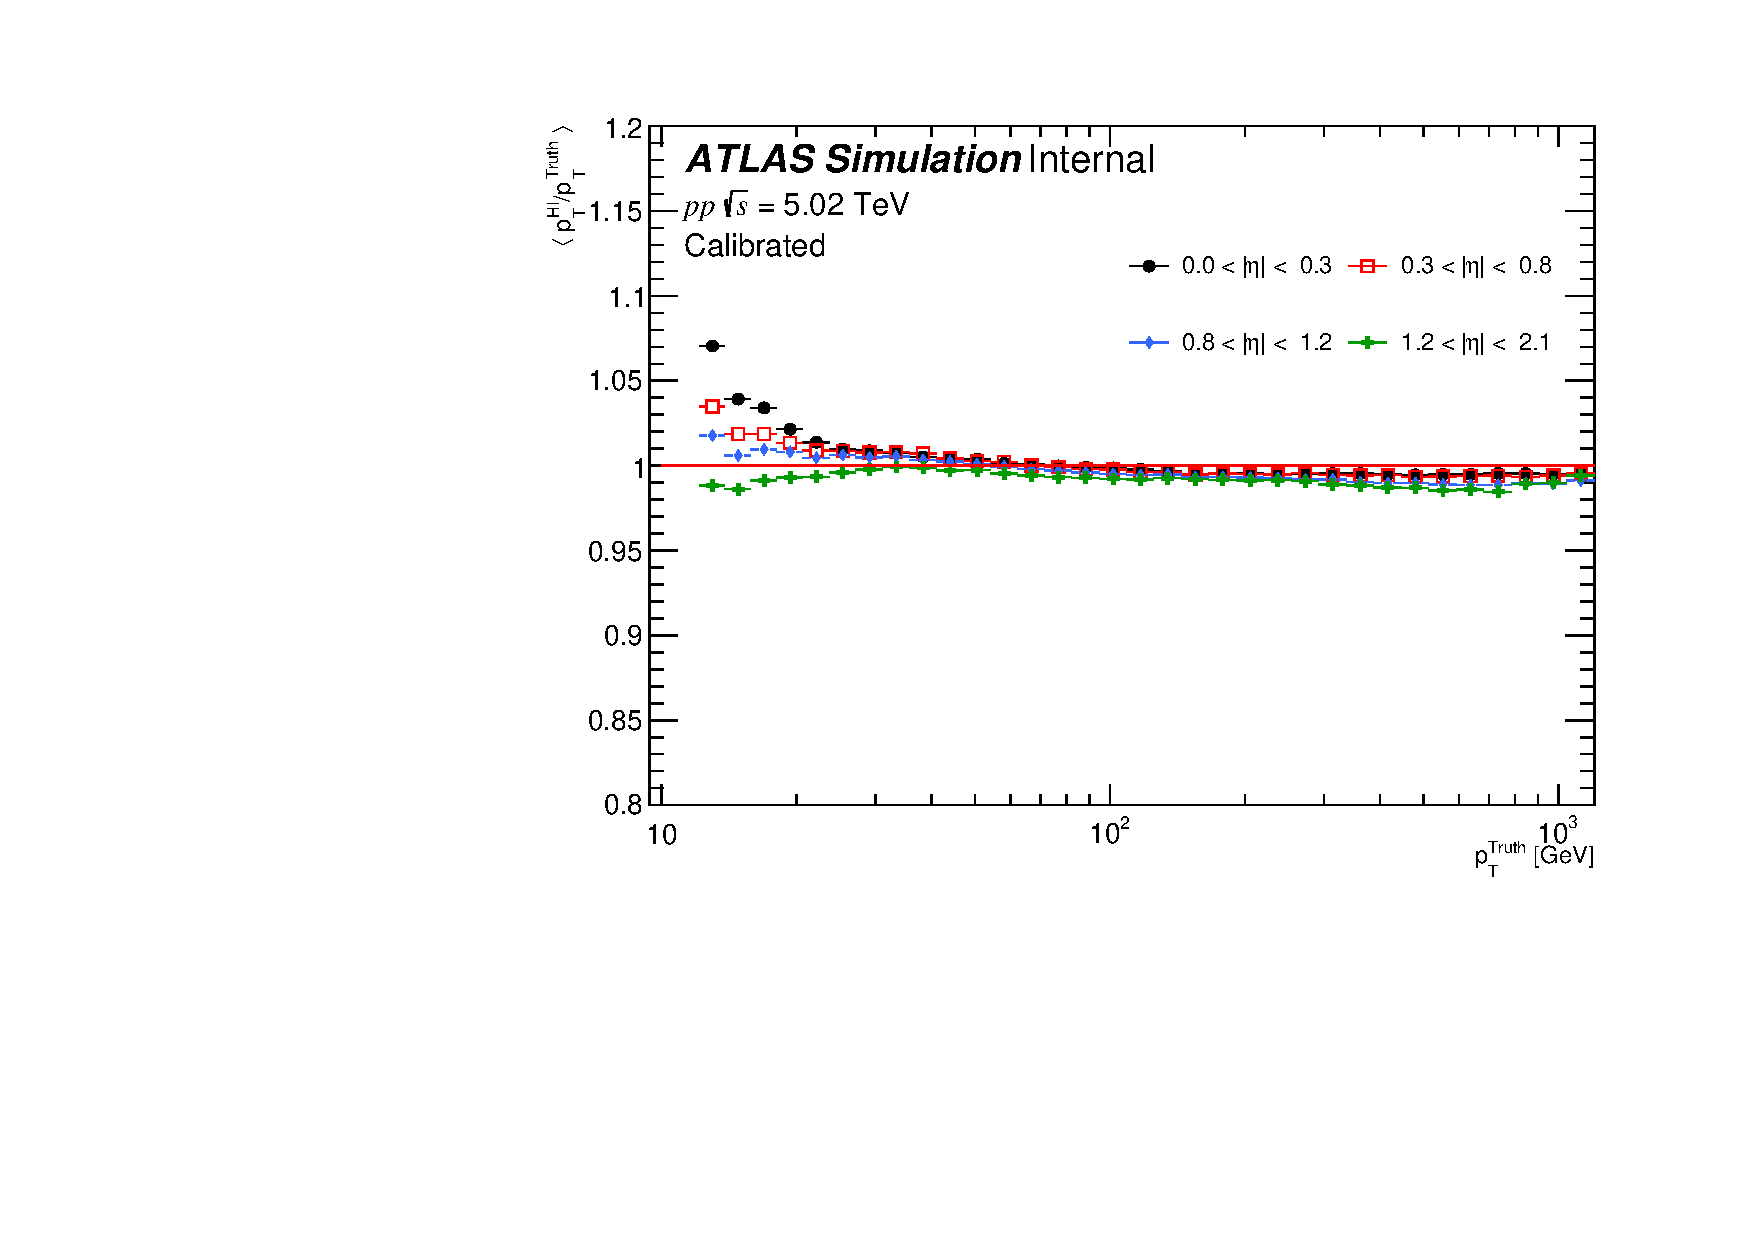
\includegraphics[width=7.3cm]{figures/main/general/JES_pp5.pdf} \\
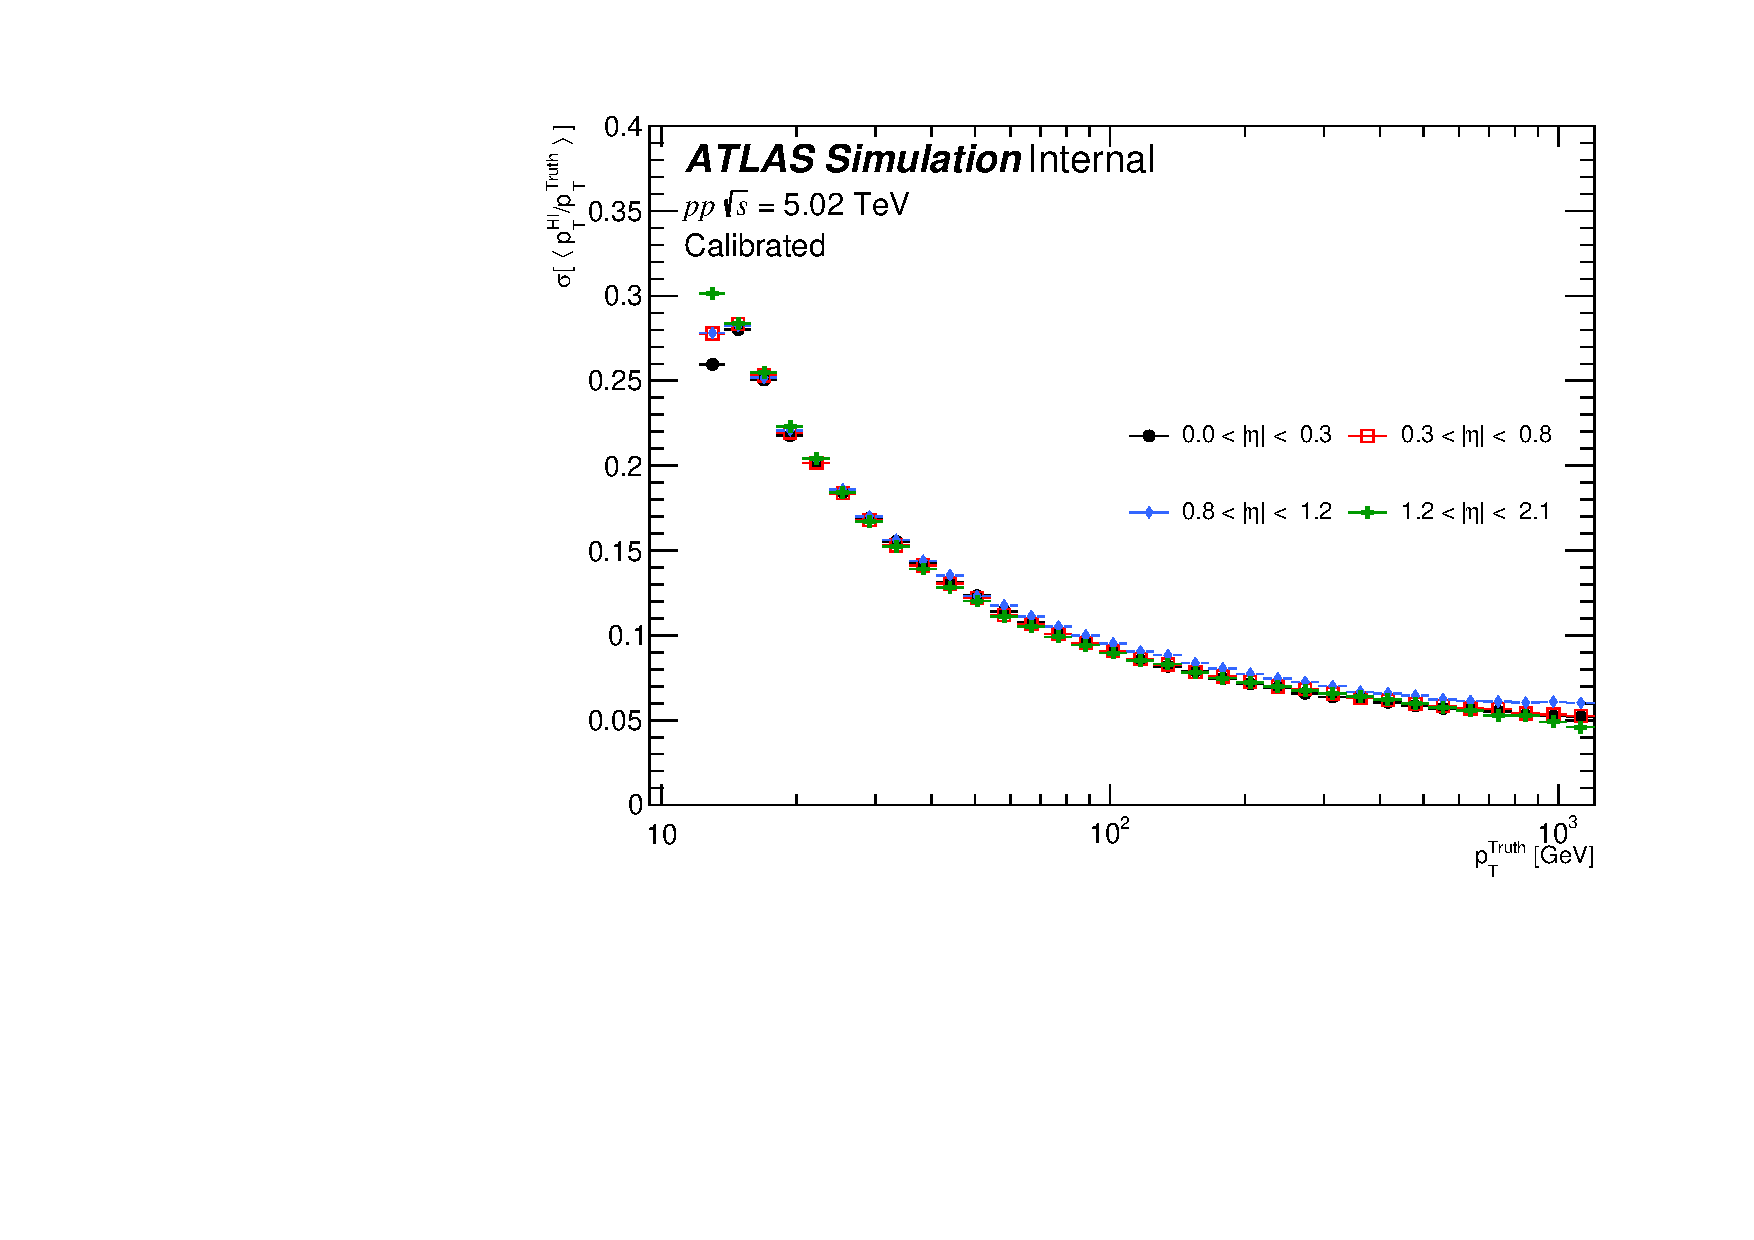
\includegraphics[width=7.3cm]{figures/main/general/JER_pp5.pdf} 
\end{tabular}}
\caption{
Top panels: Jet reconstruction efficiency in 5.02 TeV \pp\ collisions (left) as a function of truth jet \pT\ and different $\eta$ bins. Jet energy scale (JES) in 5.02 TeV \pp\ collisions (right) as a function of truth jet \pT\ and different $\eta$ bins. Bottom panels: Jet energy resolution (JER) in 5.02 \pp\ collisions as a function of truth jet \pT\ and different $\eta$ bins.
}
\label{Fig:Performancepp5}
\end{figure}

\begin{figure}
   \centering
   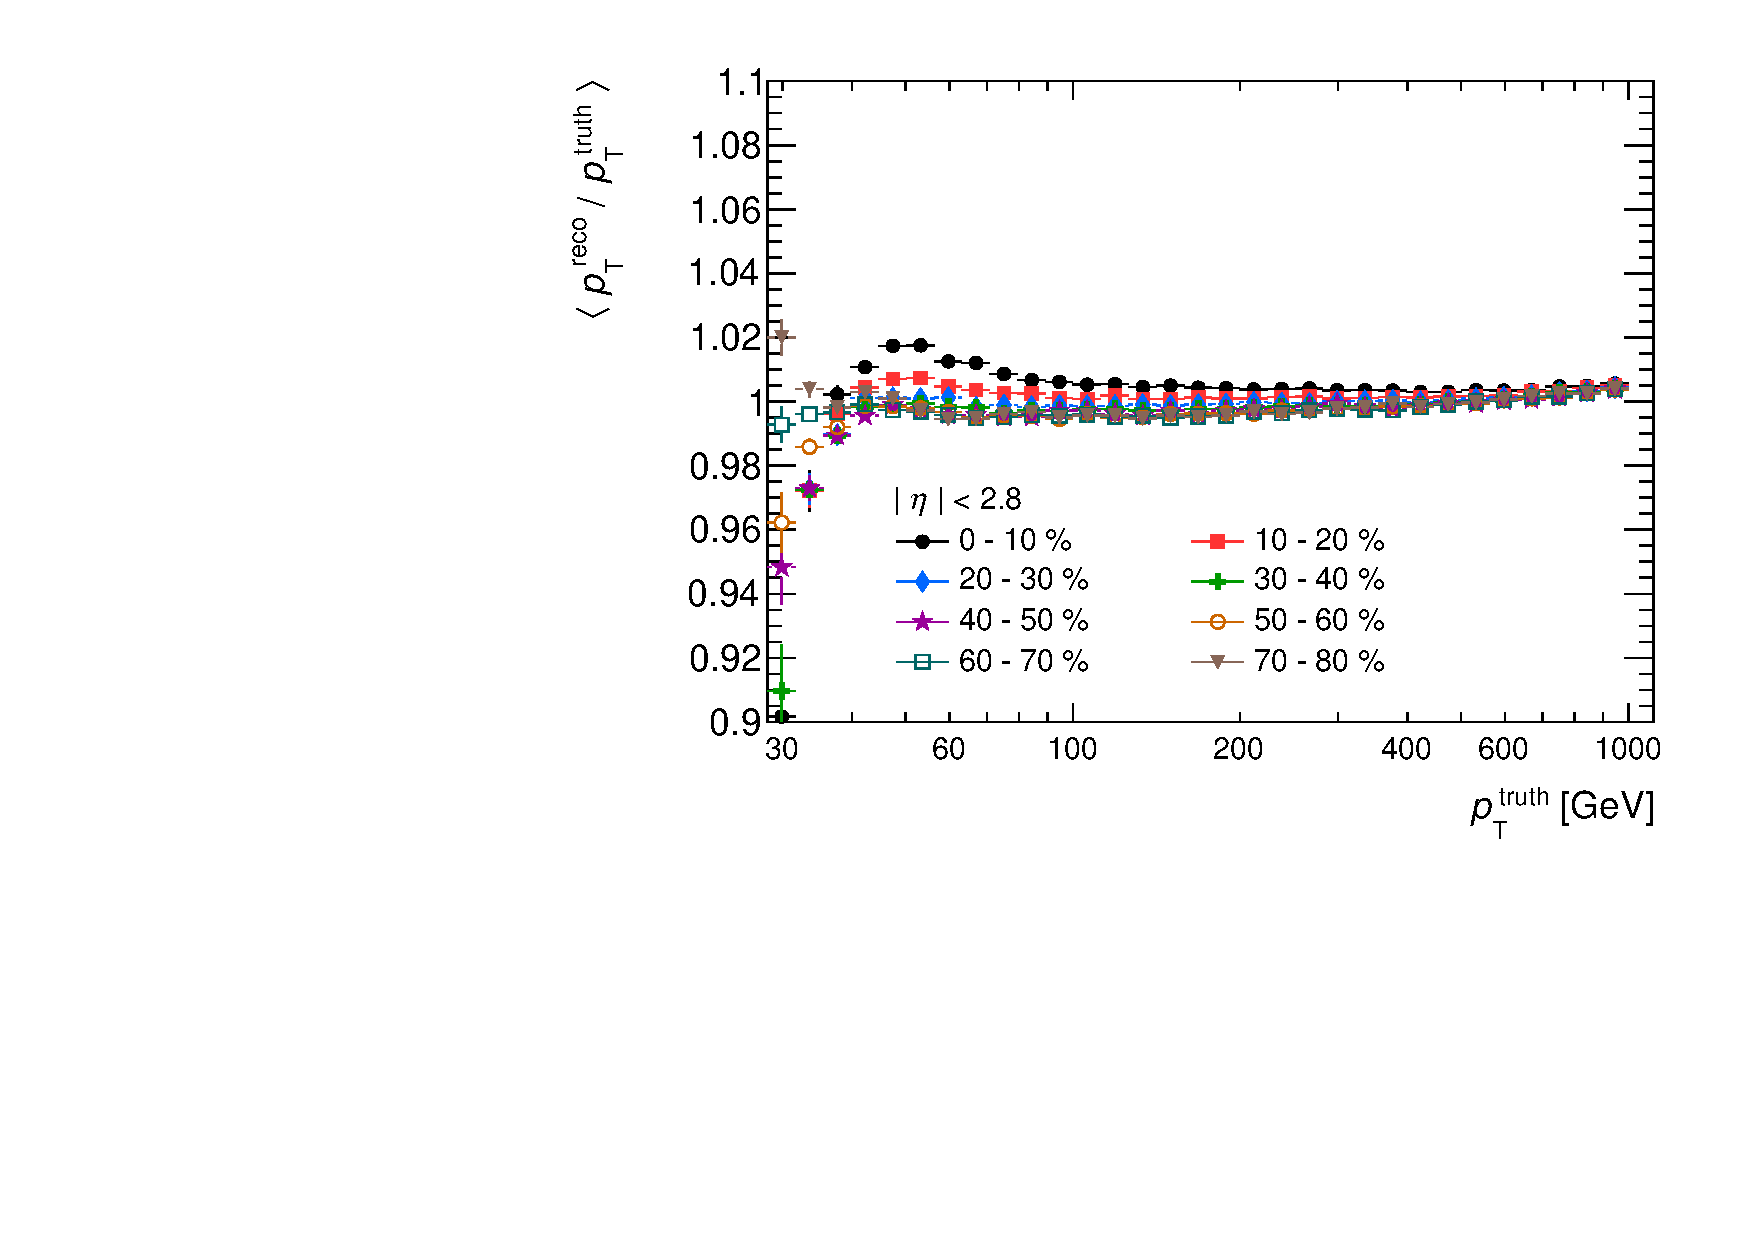
\includegraphics[width = 0.75\textwidth]{figures/main/general/PbPb_JES_pT_eta2p8.pdf}
   \caption{ JES in \pbpb\ collisions for eight centrality selections.  Plot is from Ref.~\cite{Aad:2014bxa}.}
   \label{Fig:PerformancepbpbJES}
\end{figure}

\begin{figure}
   \centering
   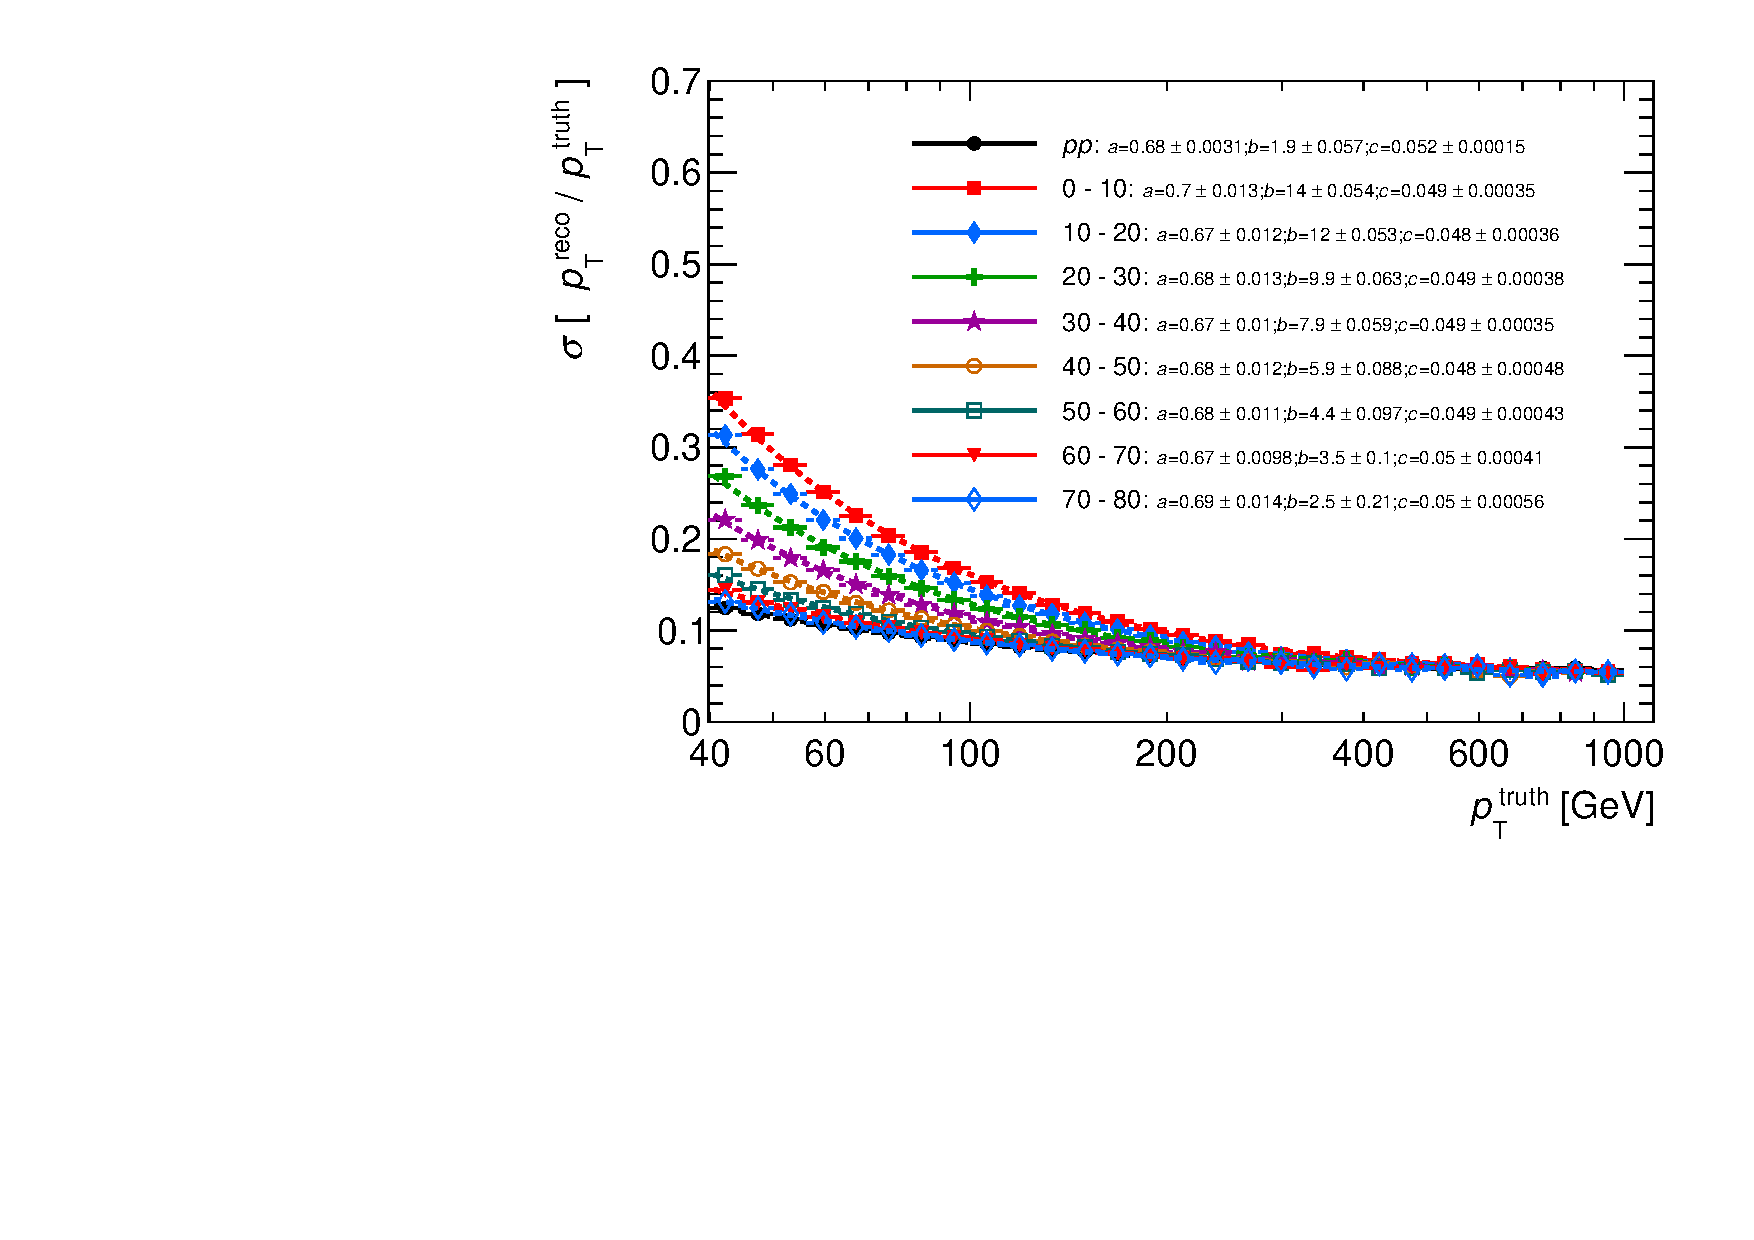
\includegraphics[width = 0.75\textwidth]{figures/main/general/PbPb_JER_pT_eta2p8.pdf}
   \caption{ JER in \pbpb\ collisions for eight centrality selections.  Plot is from Ref.~\cite{Aad:2014bxa}. The points are fit to the standard function that describes the calorimetric resolution.}
   \label{Fig:PerformancepbpbJER}
\end{figure}


\begin{figure}
   \centering
   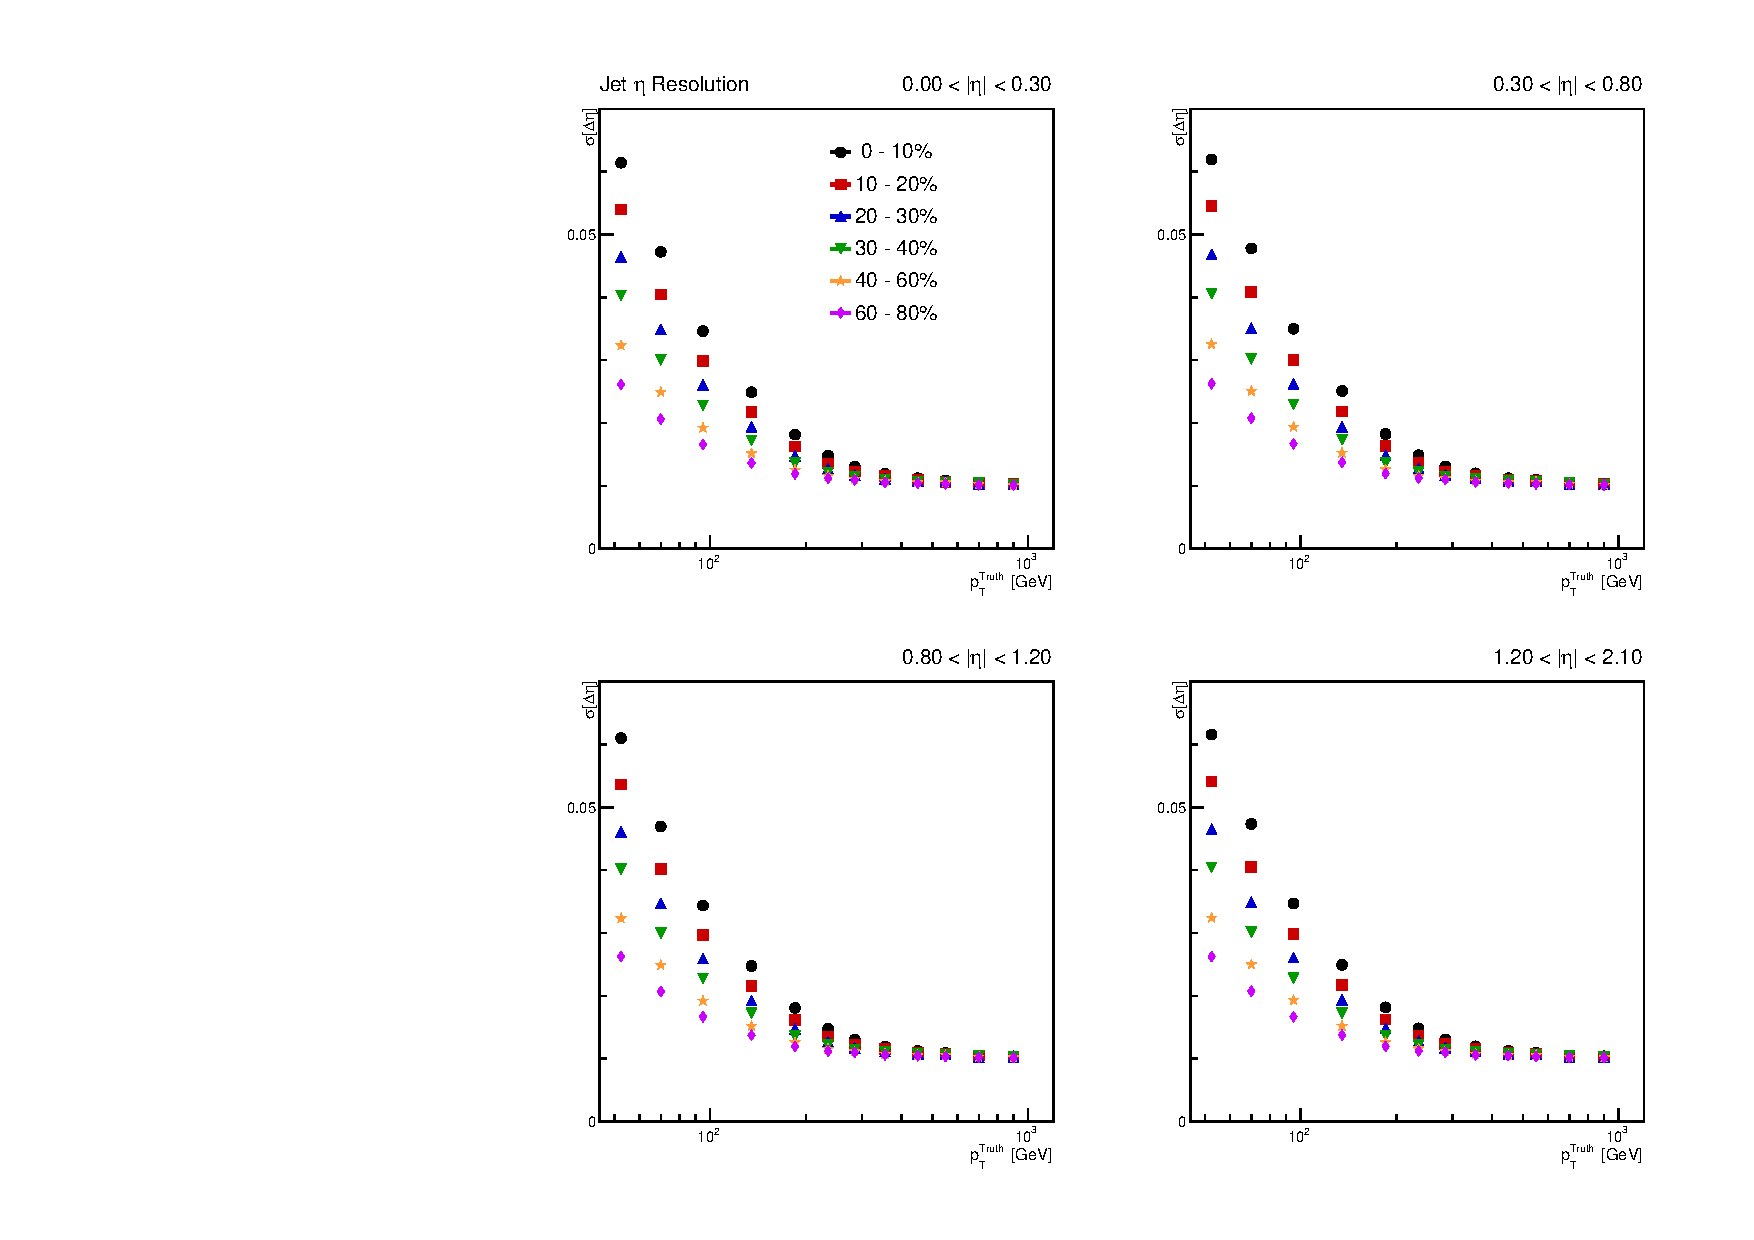
\includegraphics[width = 0.75\textwidth]{figures/main/general/jet_res_eta_r04.pdf}
   \caption{ Jet angular resolution in $\eta$ for $R=0.4$ jets in \pbpb\ collisions as a function of jet \pT\ for six centrality selections.}
   \label{Fig:PerformancepbpbJPReta0p4}
\end{figure}

\begin{figure}
   \centering
   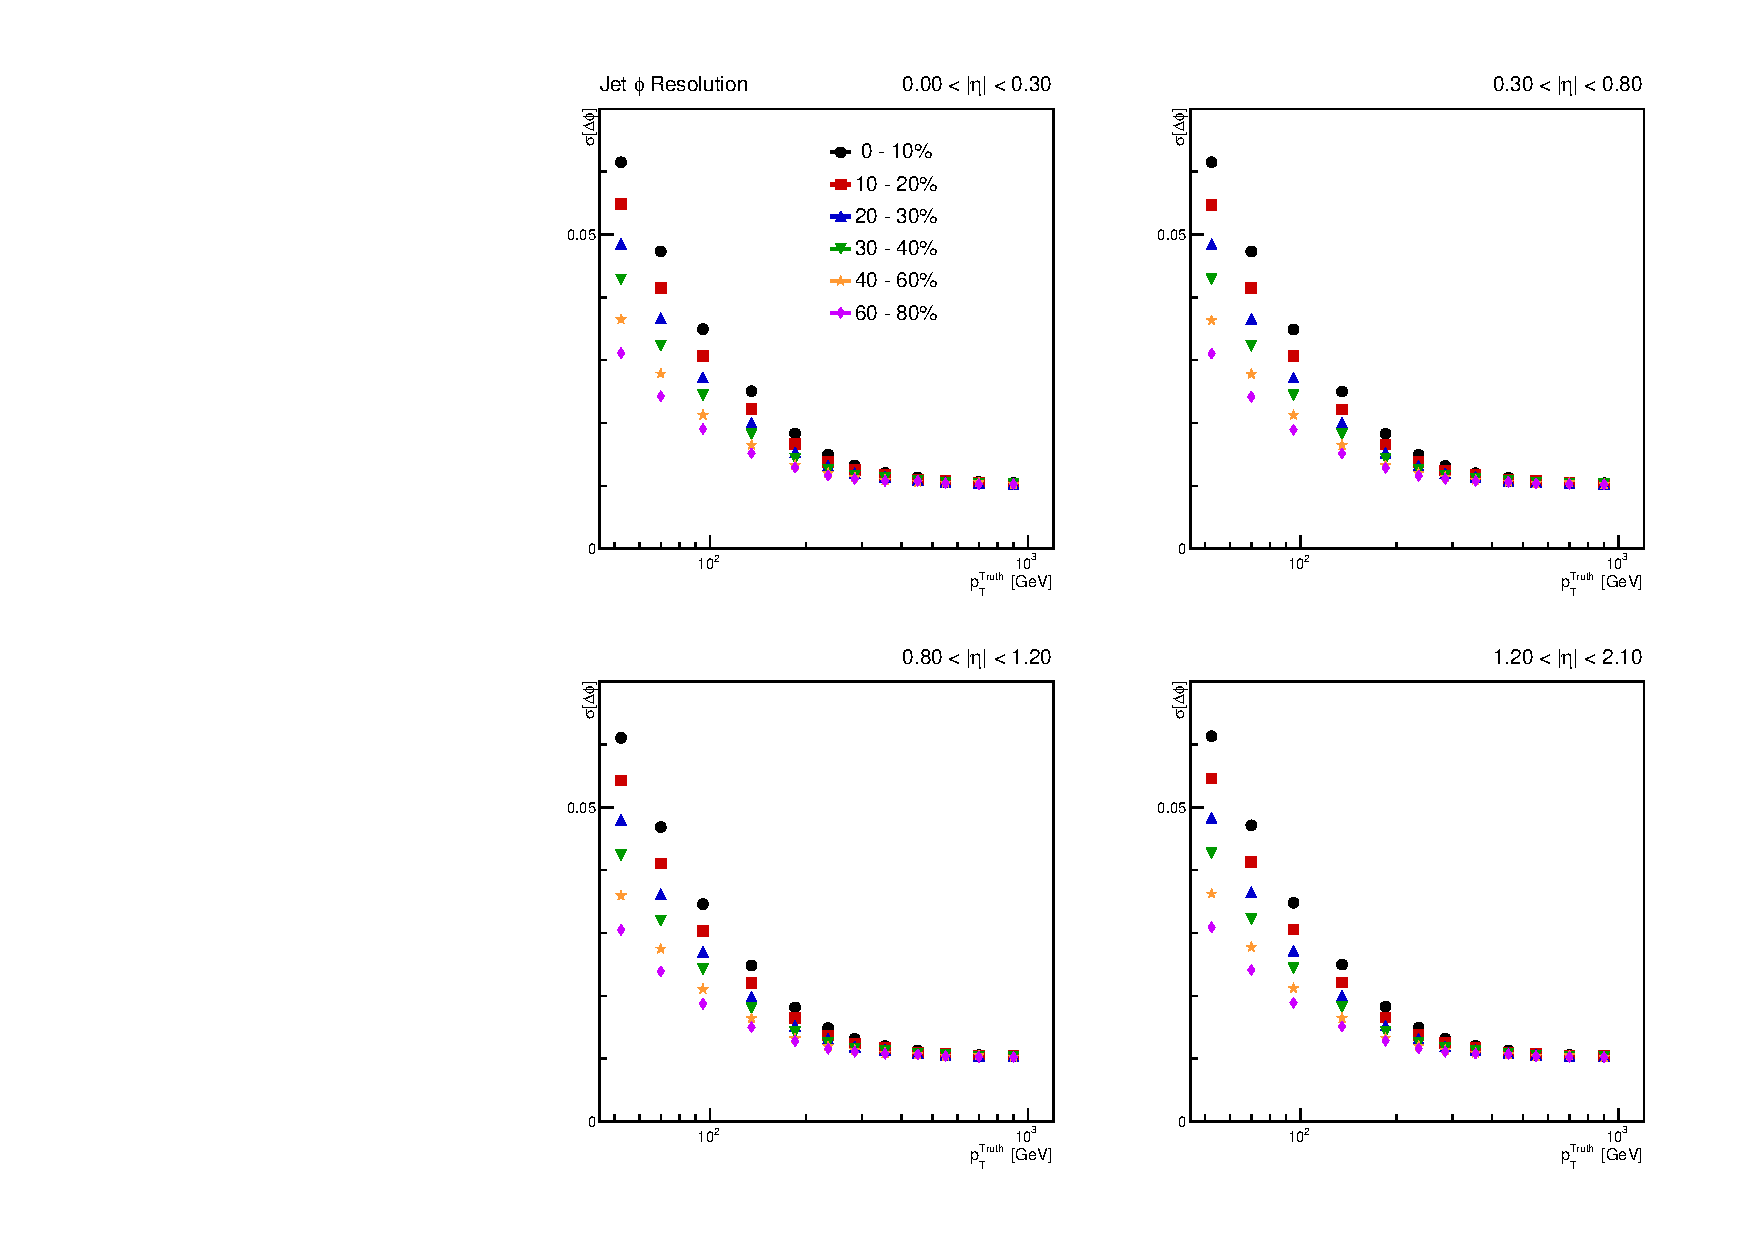
\includegraphics[width = 0.75\textwidth]{figures/main/general/jet_res_phi_r04.pdf}
   \caption{ Jet angular resolution in $\phi$ for $R=0.4$ jets in \pbpb\ collisions as a function of jet \pT\ for six centrality selections.}
   \label{Fig:PerformancepbpbJPRphi0p4}
\end{figure}



\section{Basic Cuts and Corrections}
\label{sec:cuts_corrections}
% !TEX encoding = UTF-8 Unicode
% !TEX root = thesis-ex.tex

A description of the analysis procedure to reconstruct the $\Dptr$ distribution, along with the derivation and application of the various corrections is presented in the following sections.
The analysis structure is illustrated by the diagram in Figure~\ref{fig:analysis_flow} where each part of the analyses is described in a separate subsection and can be summarized as follows: 


\begin{figure}
\centering
\includegraphics[width=0.6\textwidth]{figures/main/general/Shape_analyses_flow}
\caption{The diagram presents various corrections and cuts that are applied during the analysis.}
\label{fig:analysis_flow}
\end{figure}


\begin{itemize}
\item Jet selection
\item Track selection
\item Track momentum correction
\item Fake rates
\item Tracking efficiency
\item Underlying event subtraction of tracks
\item Unfolding
\end{itemize}




%%%%%%%%%%%%%%%%%%%%%%%%%%%%%%
\subsection{Jet Selection and final energy calibration}
\label{Sec:JetSelection}
Since the Inner Detector (ID) covers the $|\eta| < 2.5$, the analysis can only be performed for jets within the pseudorapidity interval of $|\eta| < 1.7$ to have the entire $ r = $ 0.8 cone under investigation fully covered by the tracking detector.
In both collision systems, jets are measured with \ptjet\ between 126~GeV and 316~GeV in following four successive intervals: 126--158, 158--200, 200--251, and 251--316~GeV.
The \ptjet\ cut is chosen so as to exclude the contribution of ``UE jets'' generated by fluctuations in the underlying event.
This binning is also used in previous heavy ion jet measurements such as Ref.~\cite{PhysRevC.98.024908}.

Truth jets were associated with the nearest reconstructed jet using the matching of $\dR<0.2$ for the performance study and to build response matrices for the unfolding procedure.
The same \dR\ matching criteria were employed in previous ATLAS HI jet analyses and are justified by a detailed performance study~\cite{ATLAS-COM-PHYS-2011-1733}.
To prevent nearby jets from distorting the measurement of \Dptr\ distributions, jets are rejected if there is a neighboring jet with higher \ptjet\ within an angular distance of $\Delta R < 1.0$.
The isolation cut removes approximately 0.01\% of jets (see Figure \ref{fig:ISO}), and has almost no impact on the final measurement.

\begin{figure}
\centering
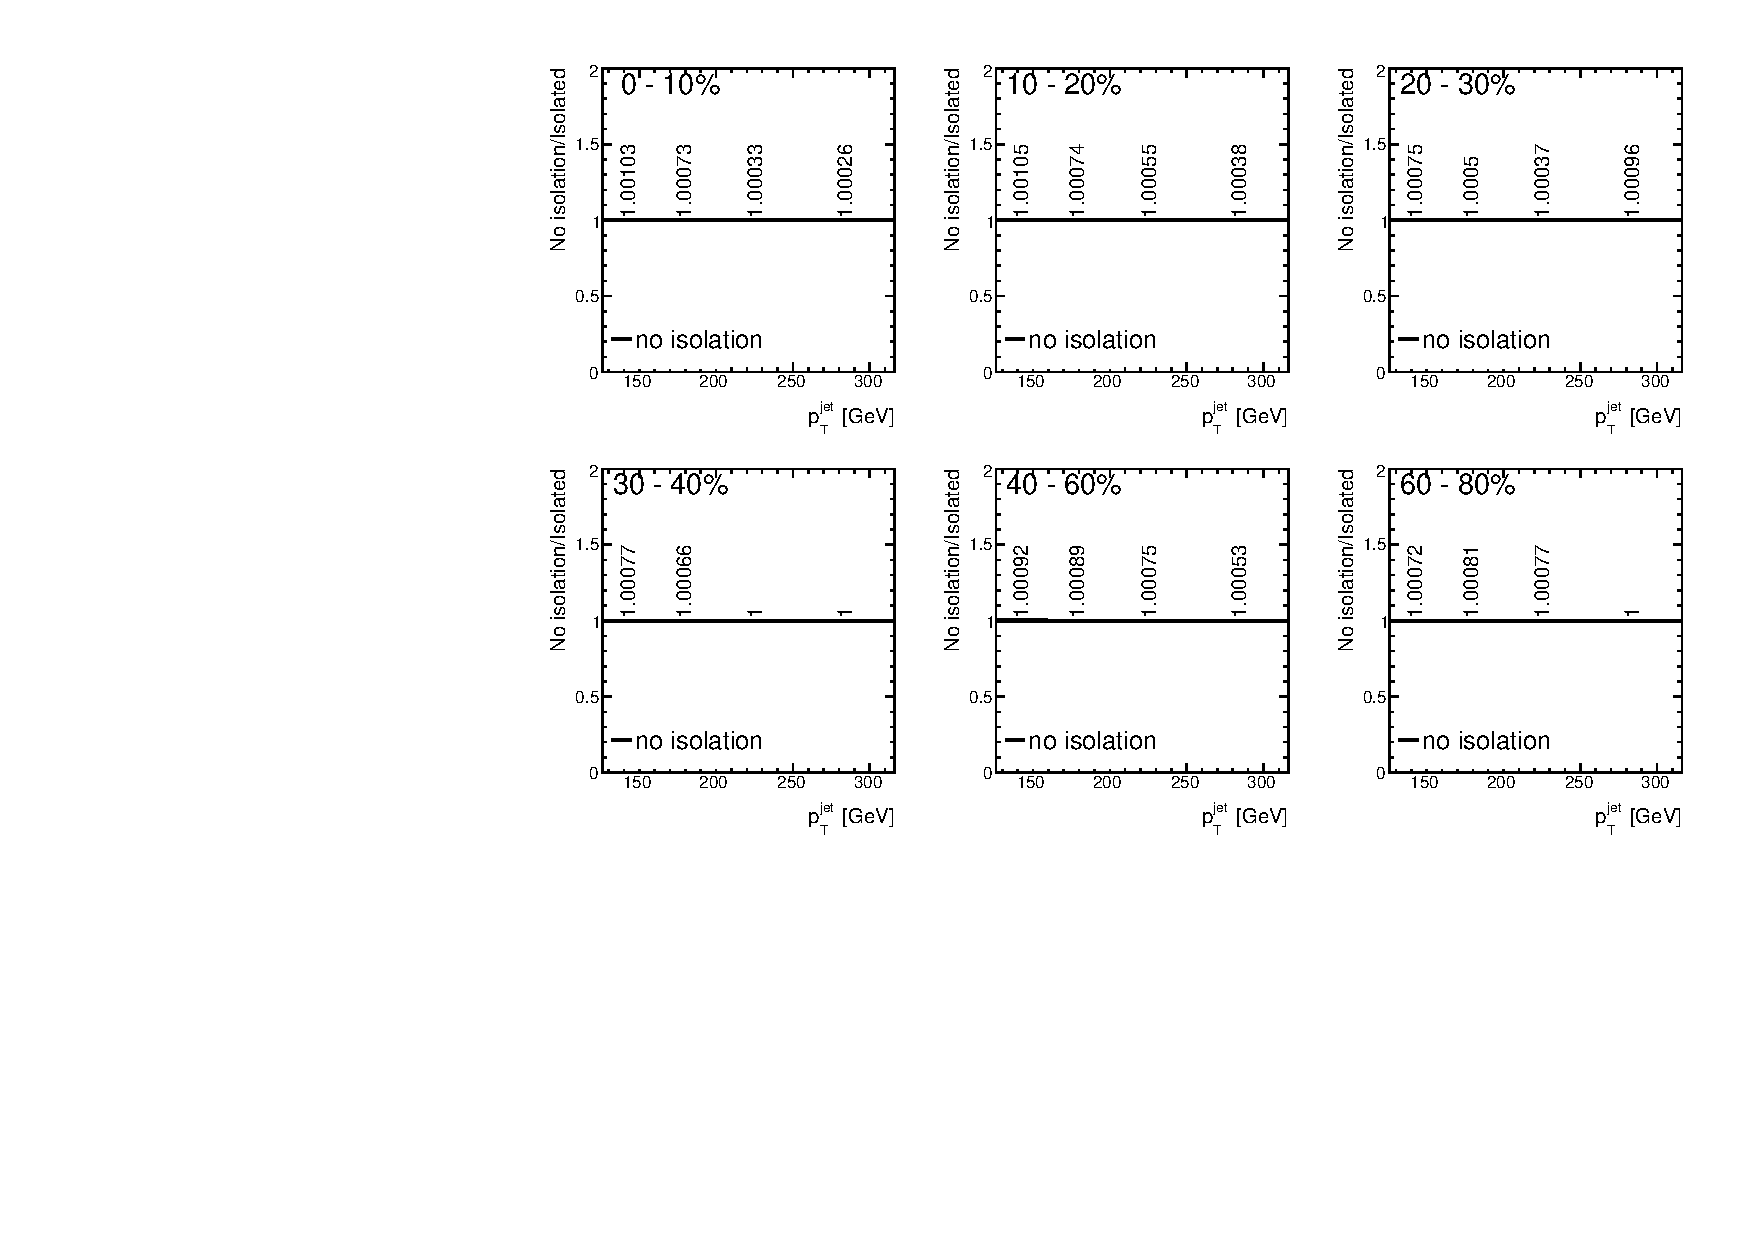
\includegraphics[width=0.9\textwidth]{figures/main/performance/jet_iso.pdf}
\caption{The ratios of the jet spectra with no isolation to that with isolation in the kinematic range of interest for \pbpb\ collisions, in all centralities.
The isolation requirement rejects less that 0.1\% of jets, and has almost no impact on the final measurement.
}
\label{fig:ISO}
\end{figure}  

No correction for the jet reconstruction efficiency is necessary, as the analysis is performed in the jet \pT\ region where the jet reconstruction is fully efficient~\cite{2015392}.
The jet energy measured in the calorimeter can be affected by the presence of dead cells or cells with a bad response, by noise spikes in the hadronic end-cap, by a noise in EM calorimeter and by out-of-time energy deposits from cosmic rays and beam backgrounds.
In the \pp\ analysis, the set of recommended cuts of ``LooseBad'' is used to remove bad jets.
The rate of these jets in the kinematic region of interest (100--316 \GeV) is less than 0.5\%.
This cleaning procedure is not applied in \PbPb\ collisions because it is incompatible with the heavy ion jet reconstruction procedure, and also because the low luminosity ensures noise bursts are negligible.
This is standard procedure for all heavy ion jet analyses.


%%%%%%%%%%%%%%%%%%%%%%%%%%%%%%
\subsection{Track selection}
\label{sec:trackselection}

The track selection cuts used here follow the cuts used in~\cite{PhysRevC.98.024908}.
These provide a low level of fake tracks and a track reconstruction efficiency that is independent of the \pt\ of the jet the track is associated with.

The cuts used here are the ``tight" cuts as described in Ref.~\cite{ref:tracktwiki} and were utilized in previous HI jet fragmentation measurements.
The default tracking cuts used both in \pp\ and \PbPb\ analysis are:
\begin{itemize}
\item{ track $\pT>$~1~GeV}
\item{ track $|\eta|<$~2.5}
\item{ tracks should have at least 9 silicon hits in $|\eta|\leq1.65$}
\item{ tracks should have at least 11 silicon hits in $|\eta|>1.65$}
\item{ tracks should have at least 1 hit in IB-layer + B-layer.}
\item{ tracks should have a IB-layer hit if it is expected, that is, if the track passed an active module.}
\item{ tracks should have a B-layer hit if it is expected and IB-layer hit is not expected.}
\item{ tracks should have  less than 3 holes in silicon detectors.}
\item{ tracks should have 0 holes in pixel detector.}
\item{ impact parameters of track with respect to primary vertex:  $|d_0|<$$< 0.47\times \exp{(-0.15\times\pT)} + 0.19\times \exp{(0.00034\times\pT)}$~mm, $|z_0*\sin\theta|<$1.0~mm.
Recommended values are  $|d_0| < 1.5$~mm for tracks with $\pt<10$~GeV and $|d_0| < 0.2$~mm for tracks with $\pt>10$~GeV.
This was chosen to guarantee a smooth behavior of the $d_{0}$ parameter as a function of track momentum.}
\item{ An additional cut on the track to jet \pT\ ratio is included.
All tracks with 

\begin{equation}
\pTch >  \ptjet + \sqrt{ (3 \times \sigma_{\mathrm{JER}}(\ptjet))^2 + (3 \times \sigma_{\mathrm{TMR}}(\pTch))^2} 
\end{equation}
are rejected from the analysis, where the TMR stands for track momentum resolution.
The purpose of this cut is to be consistent with previous fragmentation measurements ~\cite{PhysRevC.98.024908}.
It has minimal impact on this analysis because the analysis is restricted to tracks below 63 GeV and jets above 100 GeV.}
\end{itemize}


A tighter tracking selection is used for systematic studies (``tight+'' cuts).
These cuts include all of the default cuts plus a 3$\sigma$ cut on the significance of the $d_0$ and $z_0 \sin\theta$.
Figures~\ref{fig:trkdataMCcomp_pp}-\ref{fig:trkdataMCcomp_pbpb_highpt} shows comparisons of the data and MC tracking quantities in \pp\ and \pbpb\ collisions, respectively, for different track \pT\ intervals.
It can be seen that the MC describes the data well.
A 20\% discrepancy is observed for low impact parameters.
The discrepancy is present far from the values of corresponding tracking cuts.
There is a small shift in the $z0$ distribution in the MC samples.
This difference is caused by the allowance of a small difference in the $z$ position of the primary vertex in the MC overlay procedure.
However this has negligible impact on the analysis as the overall quality requirement on the pointing parameter in the $z0$ is 1~mm.
Furthermore, Figure~\ref{fig:trkdataMCcomp_pbpb_highpt} shows the same comparison for high \pt\ tracks.
All the comparisons of distributions show the same qualitative features as seen at lower \pt\ with improving pointing with increasing track \pt.
The comparison of the reconstructed \pttrk\ with the generated kinematics for tracks passing these cuts is shown in Figure~\ref{fig:momres_pp}.

\begin{figure}
\centering{
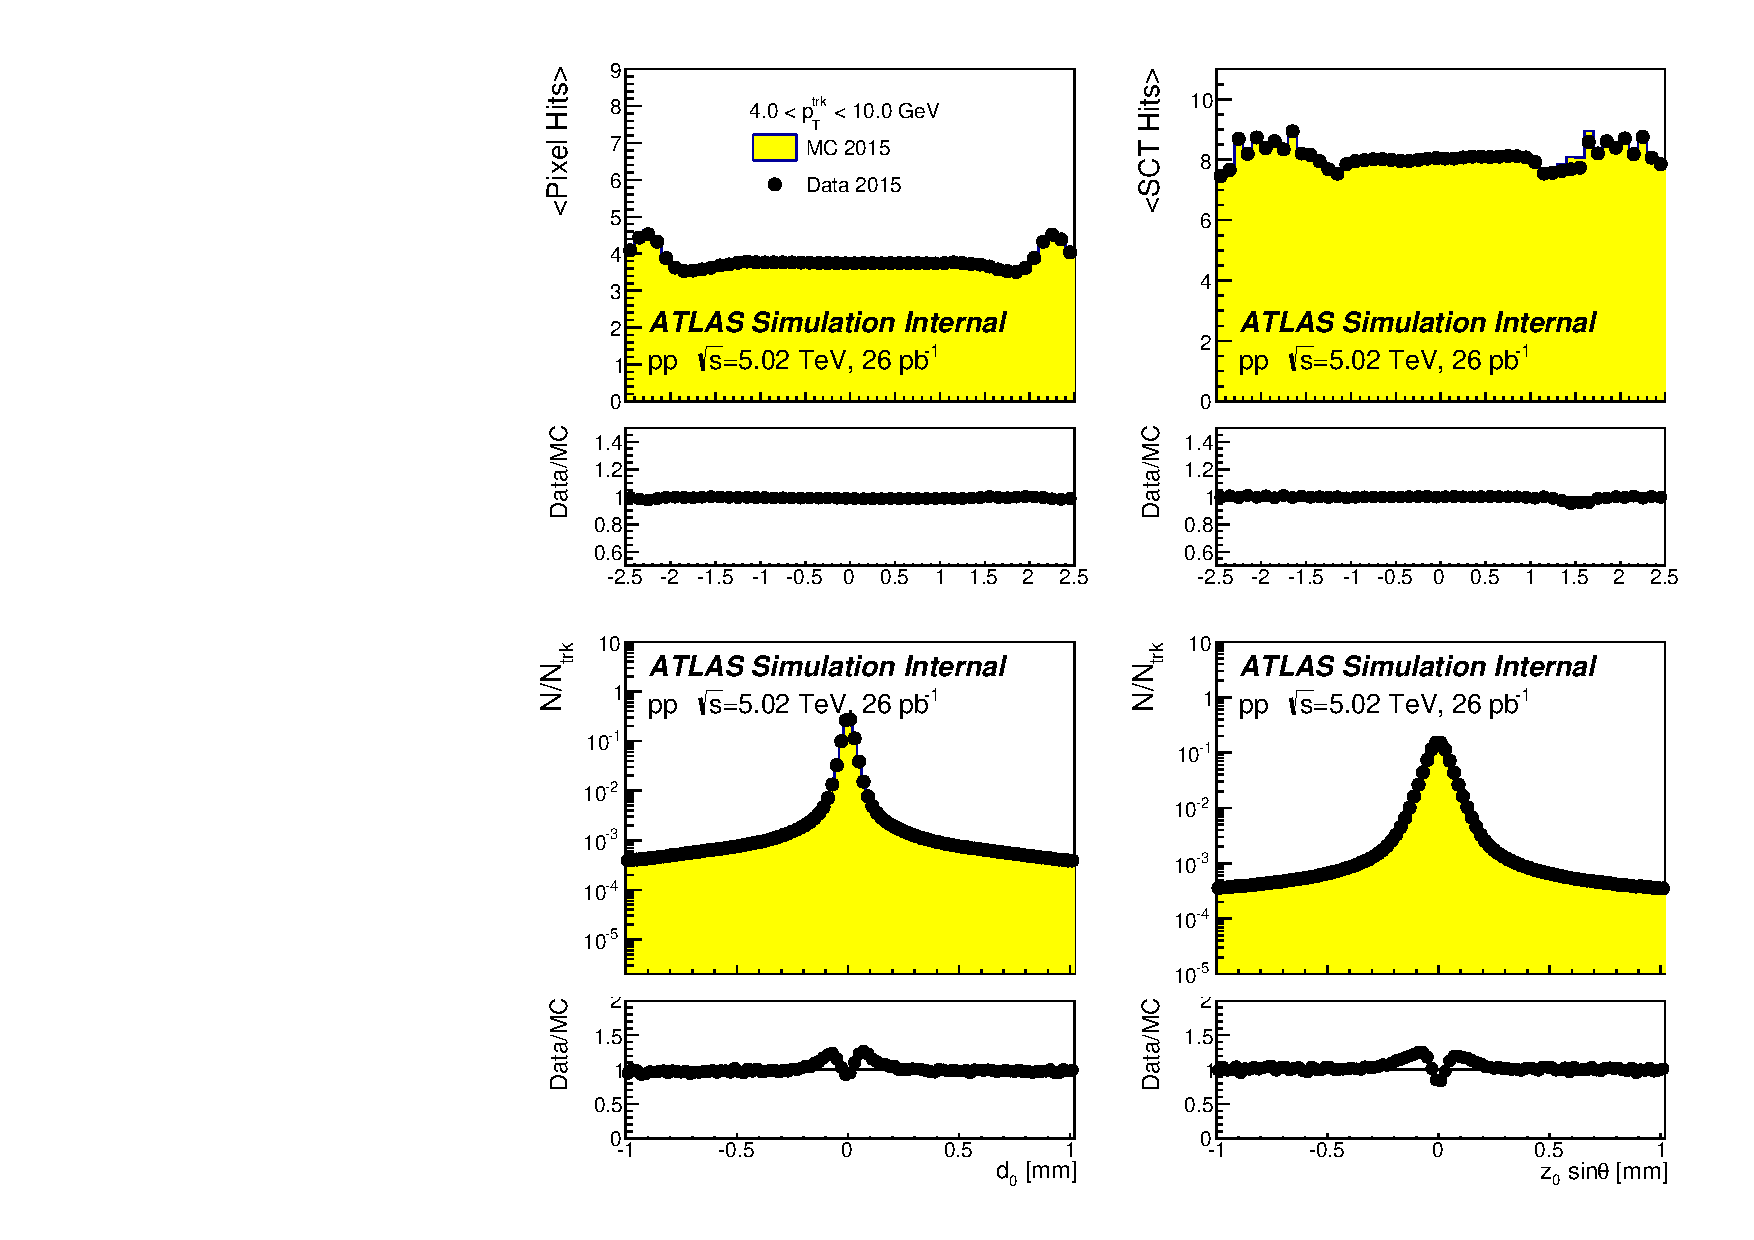
\includegraphics[width=0.75\textwidth]{figures/main/performance/TrkPerforPlots_5TeV_pp.pdf} }
\caption{Track quantity comparison between data (points) and MC (yellow histogram) in \pp\ collisions.
Tracks are selected to have 4.2~$<\pttrk<$~10~GeV.
Below each direct data and MC overlay is the corresponding data to MC ratio.
The quantities compared are: average number of pixel hits as a function of $\etatrk$ (top left), average number of SCT hits as a function of $\etatrk$ (top right), and number of tracks, $N_{\mathrm{trk}}$, normalized $d_0$ (bottom left), and $z_0 \sin\theta$ distributions (bottom right).
Figure taken from Ref.~\cite{Sickles:2235420}.}
\label{fig:trkdataMCcomp_pp}
\end{figure}

\begin{figure}
\centering{
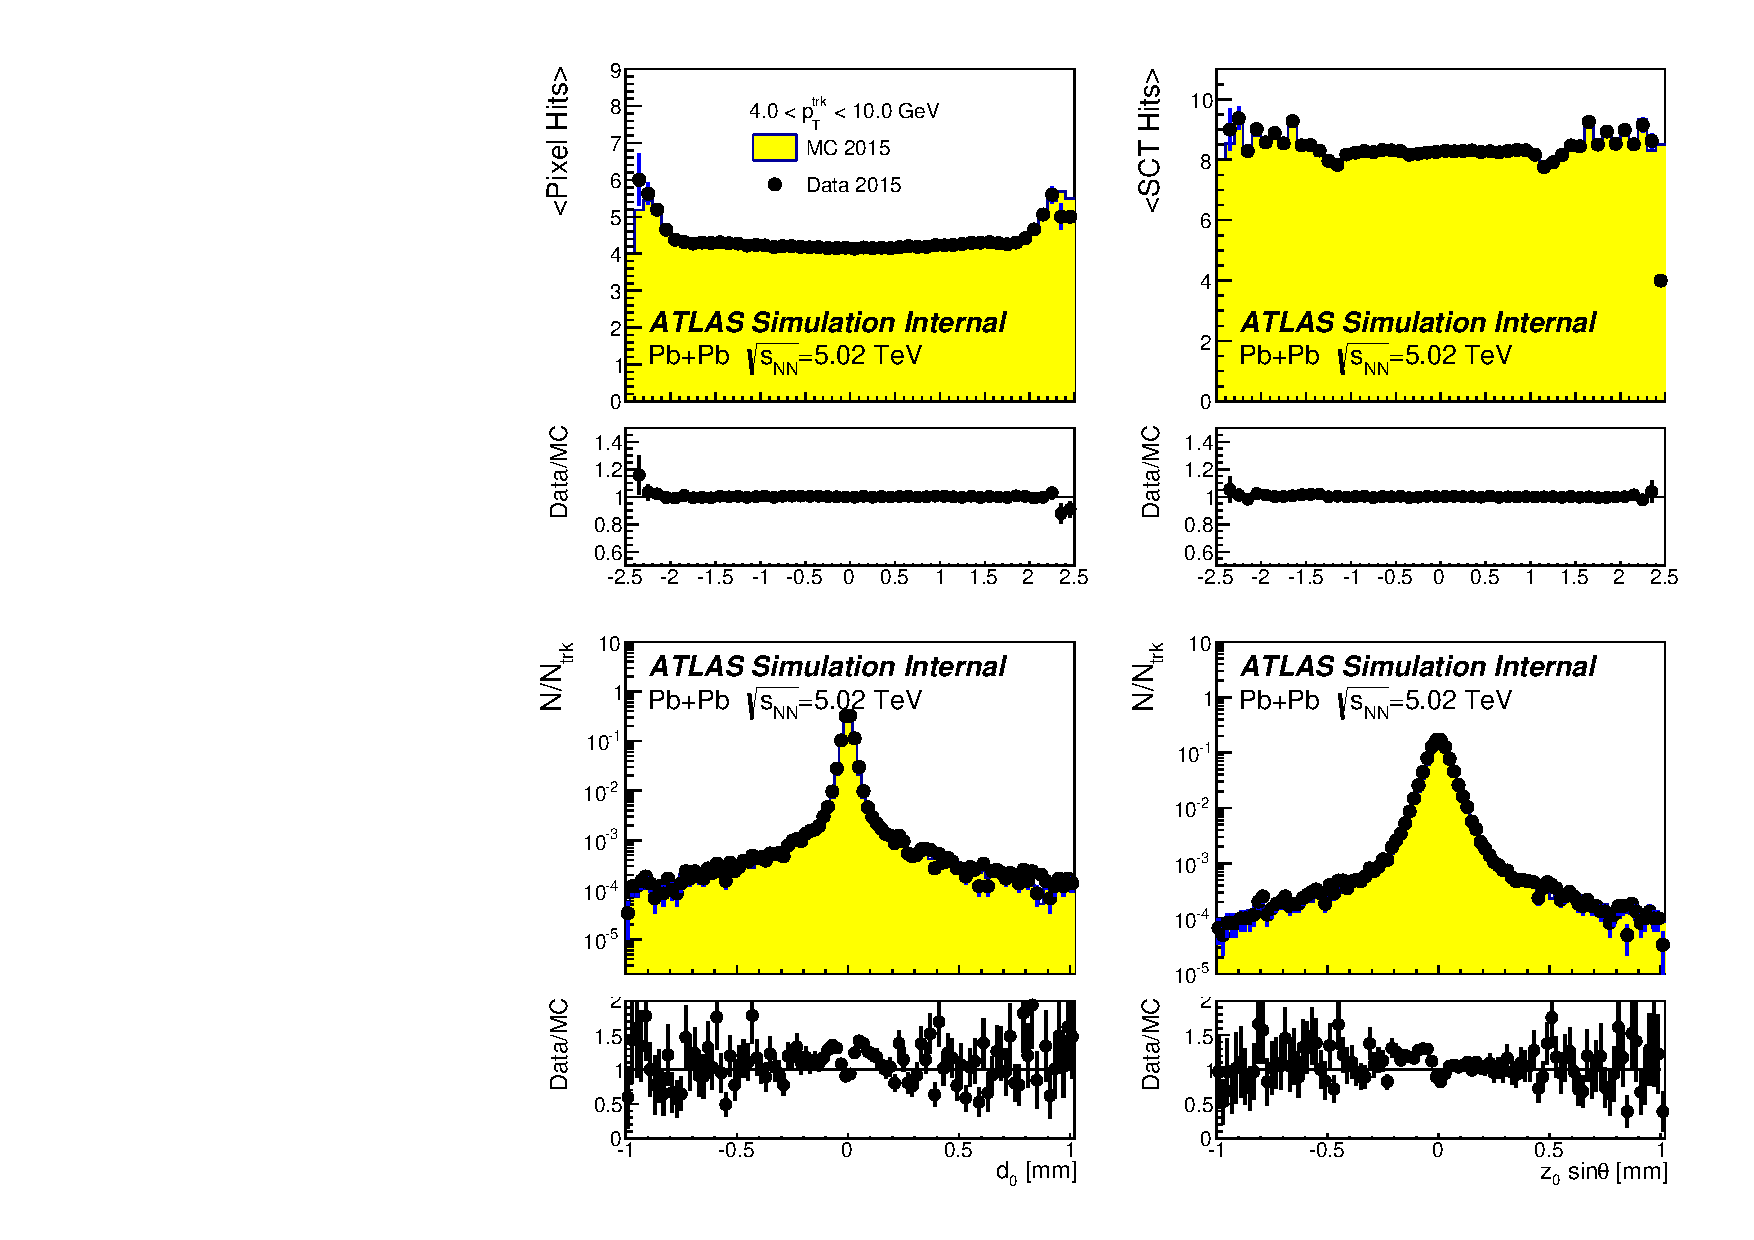
\includegraphics[width=0.75\textwidth]{figures/main/performance/TrkPerforPlots_PbPb_pt4p2_10p0GeV.pdf} }
\caption{Track quantity comparison between data (points) and MC (yellow histogram) in 0-10\% central \pbpb\ collisions.
Tracks are selected to have 4.2~$<\pttrk<$~10~GeV.
Below each direct data and MC overlay is the corresponding data to MC ratio.
The quantities compared are: average number of pixel hits as a function of $\etatrk$ (top left), average number of SCT hits as a function of $\etatrk$ (top right), track $d_0$ (bottom left), and track $z_0 \sin\theta$ (bottom right).
Figure taken from Ref.~\cite{Sickles:2235420}.}
\label{fig:trkdataMCcomp_pbpb}
\end{figure}

\begin{figure}
\centering{
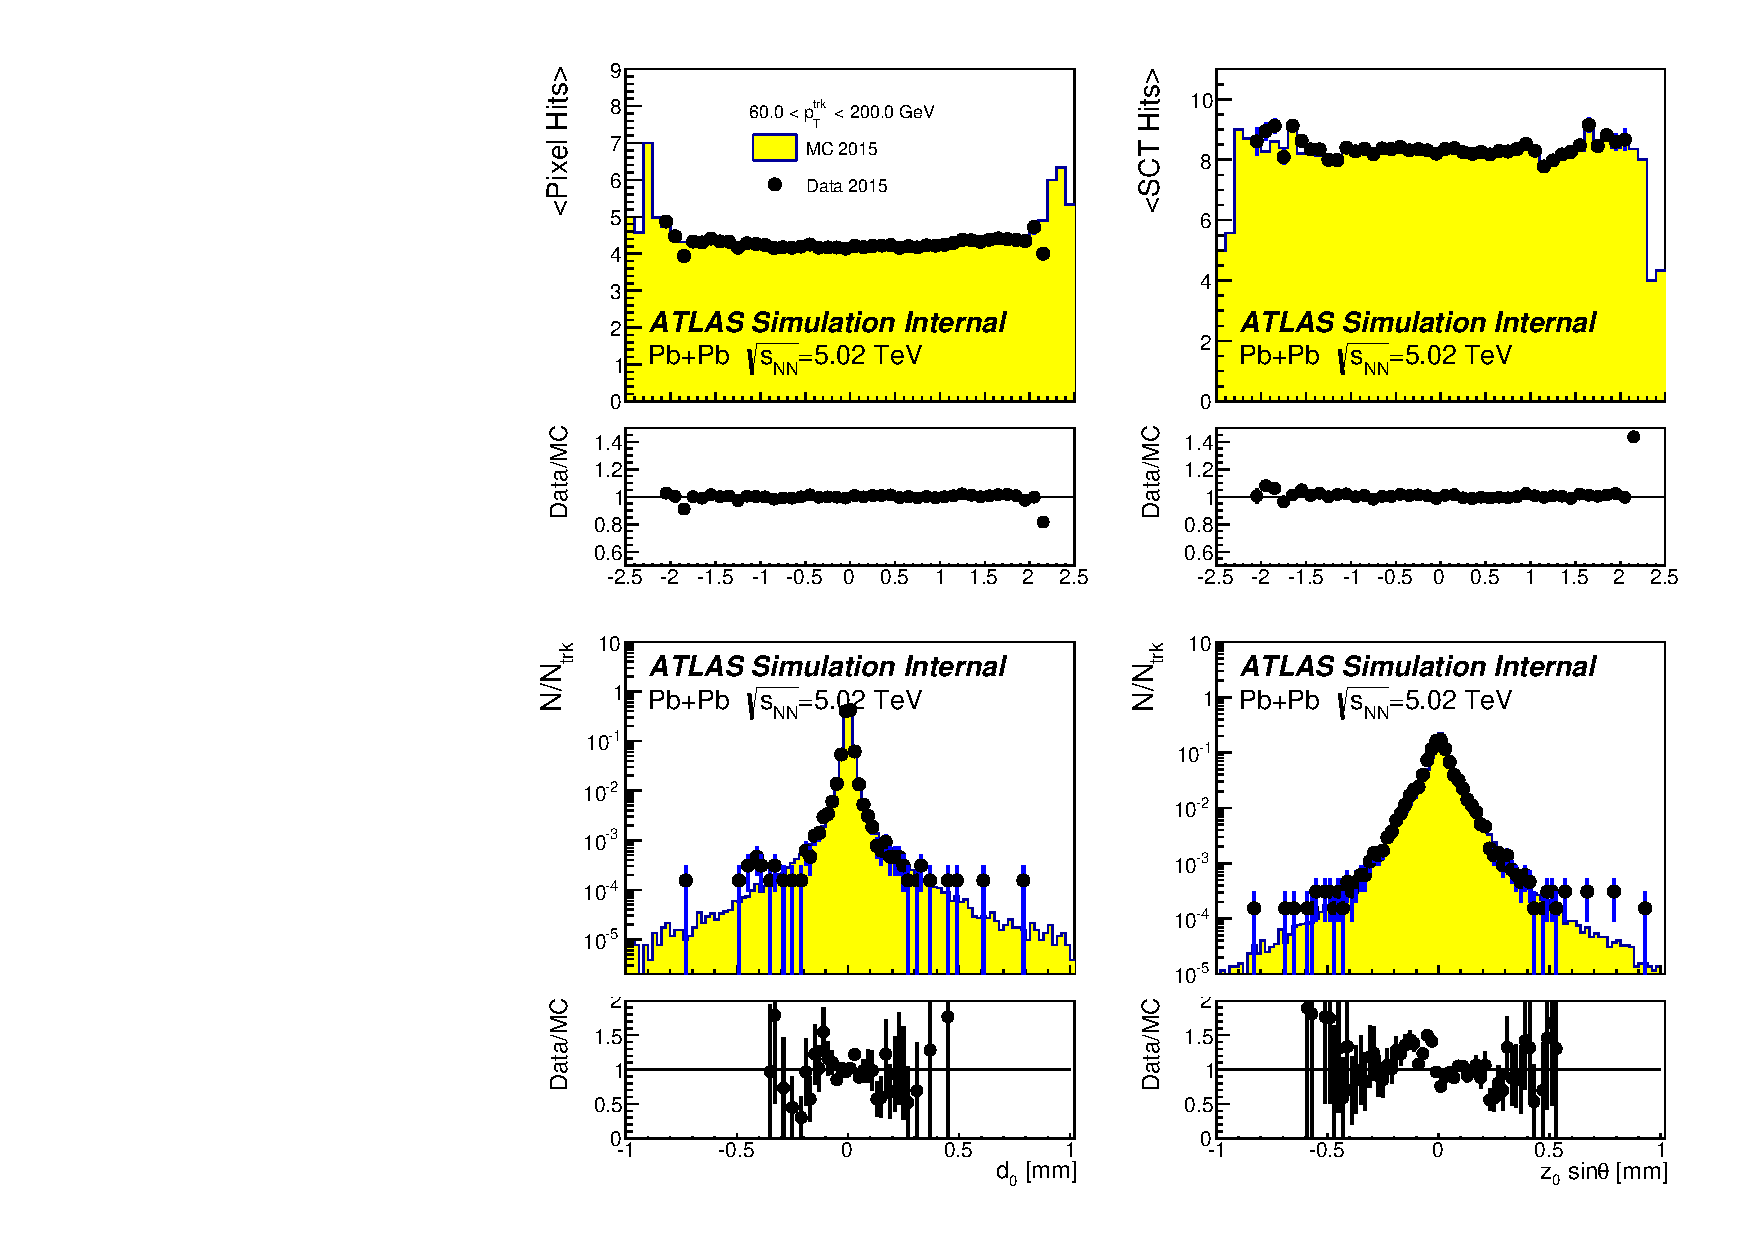
\includegraphics[width=0.75\textwidth]{figures/main/performance/TrkPerforPlots_PbPb_pt60_200GeV.pdf} }
\caption{Track quantity comparison between data (points) and MC (yellow histogram) in \pbpb\ collisions inclusive in collisions centrality.
Tracks are selected to have 60~$<\pttrk<$~200~GeV and to originate from jet with \pt\ in the interval from 251 to 316 GeV.
Below each direct data and MC overlay is the corresponding data to MC ratio.
The quantities compared are: average number of pixel hits as a function of $\etatrk$ (top left), average number of SCT hits as a function of $\etatrk$ (top right), track $d_0$ (bottom left), and track $z_0 \sin\theta$ (bottom right).
Figure taken from Ref.~\cite{Sickles:2235420}.}
\label{fig:trkdataMCcomp_pbpb_highpt}
\end{figure}


\begin{figure}
\centering{
\begin{tabular}{cc}
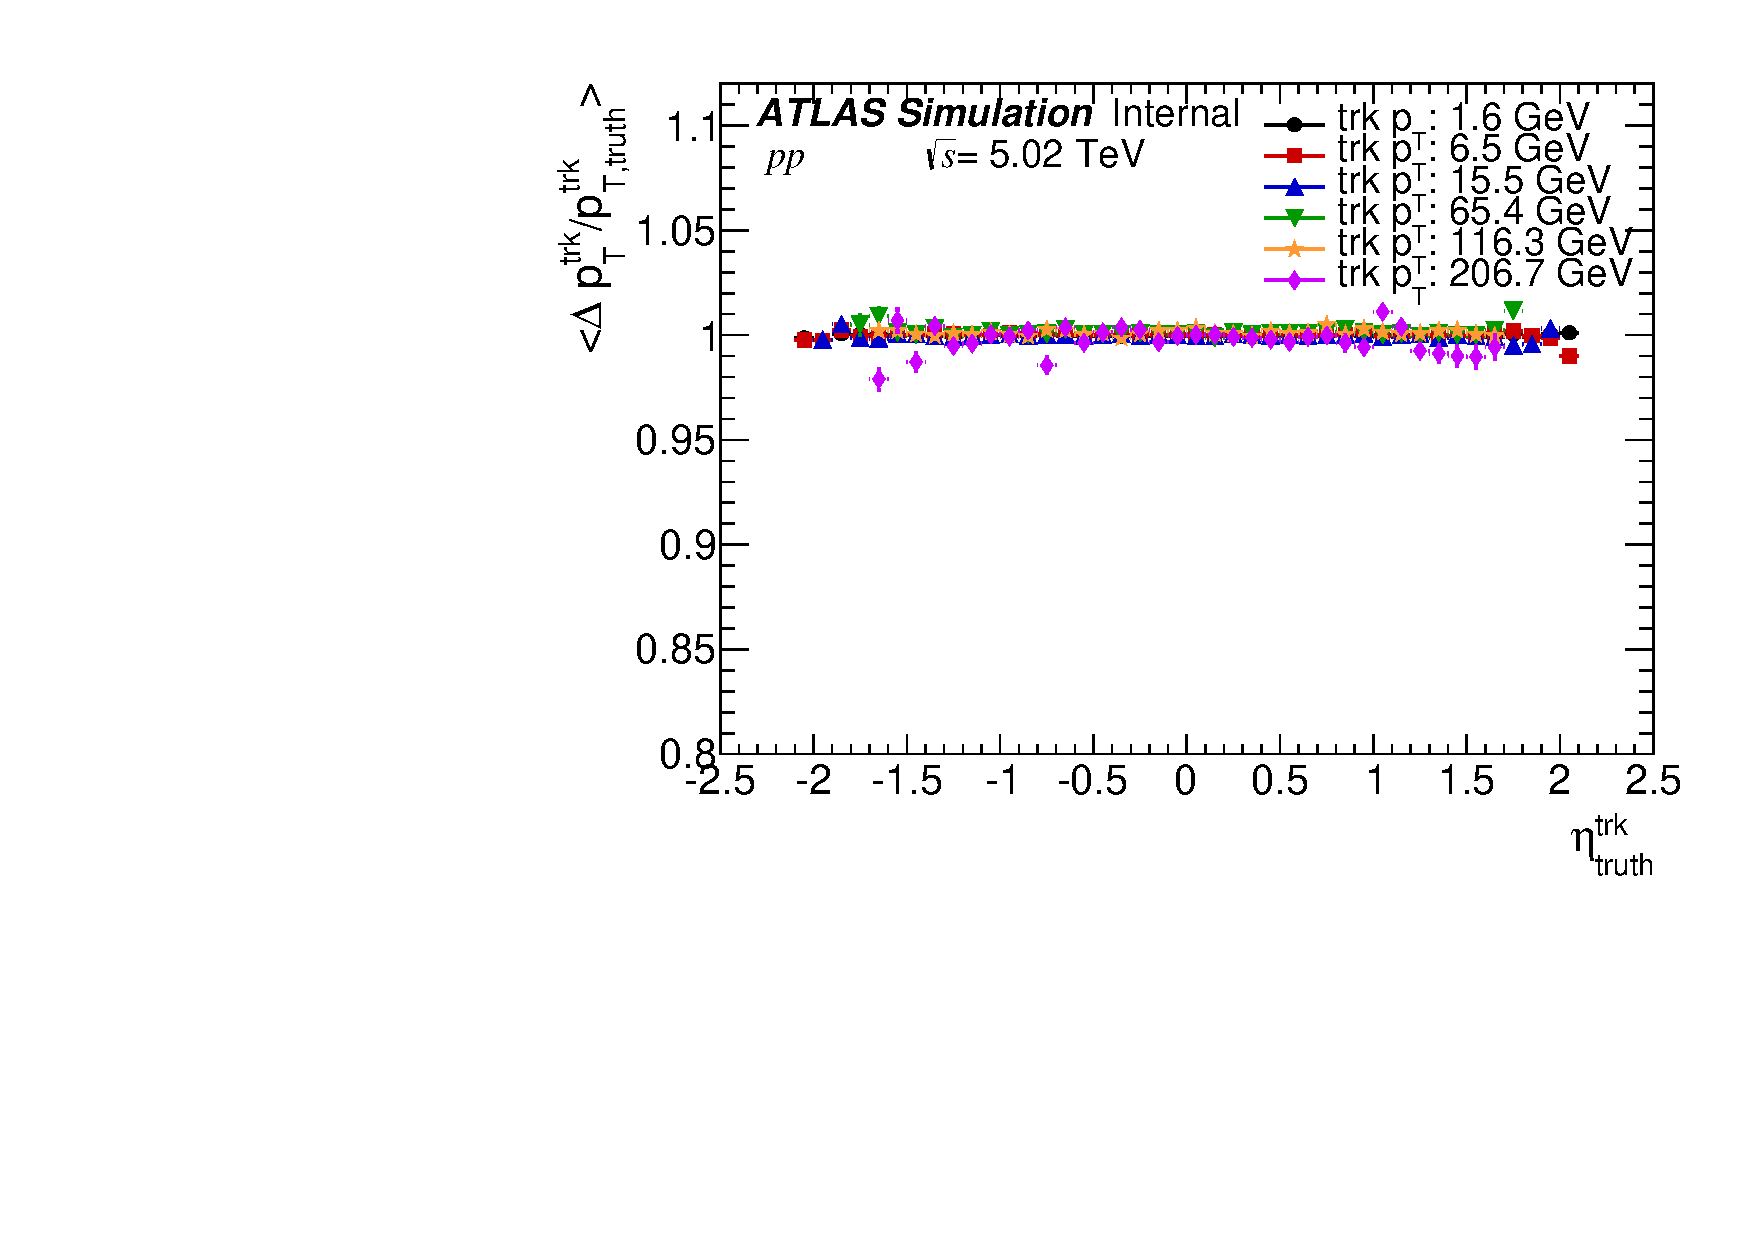
\includegraphics[width=0.45\textwidth]{figures/main/performance/scale_v_eta_pp.pdf} &
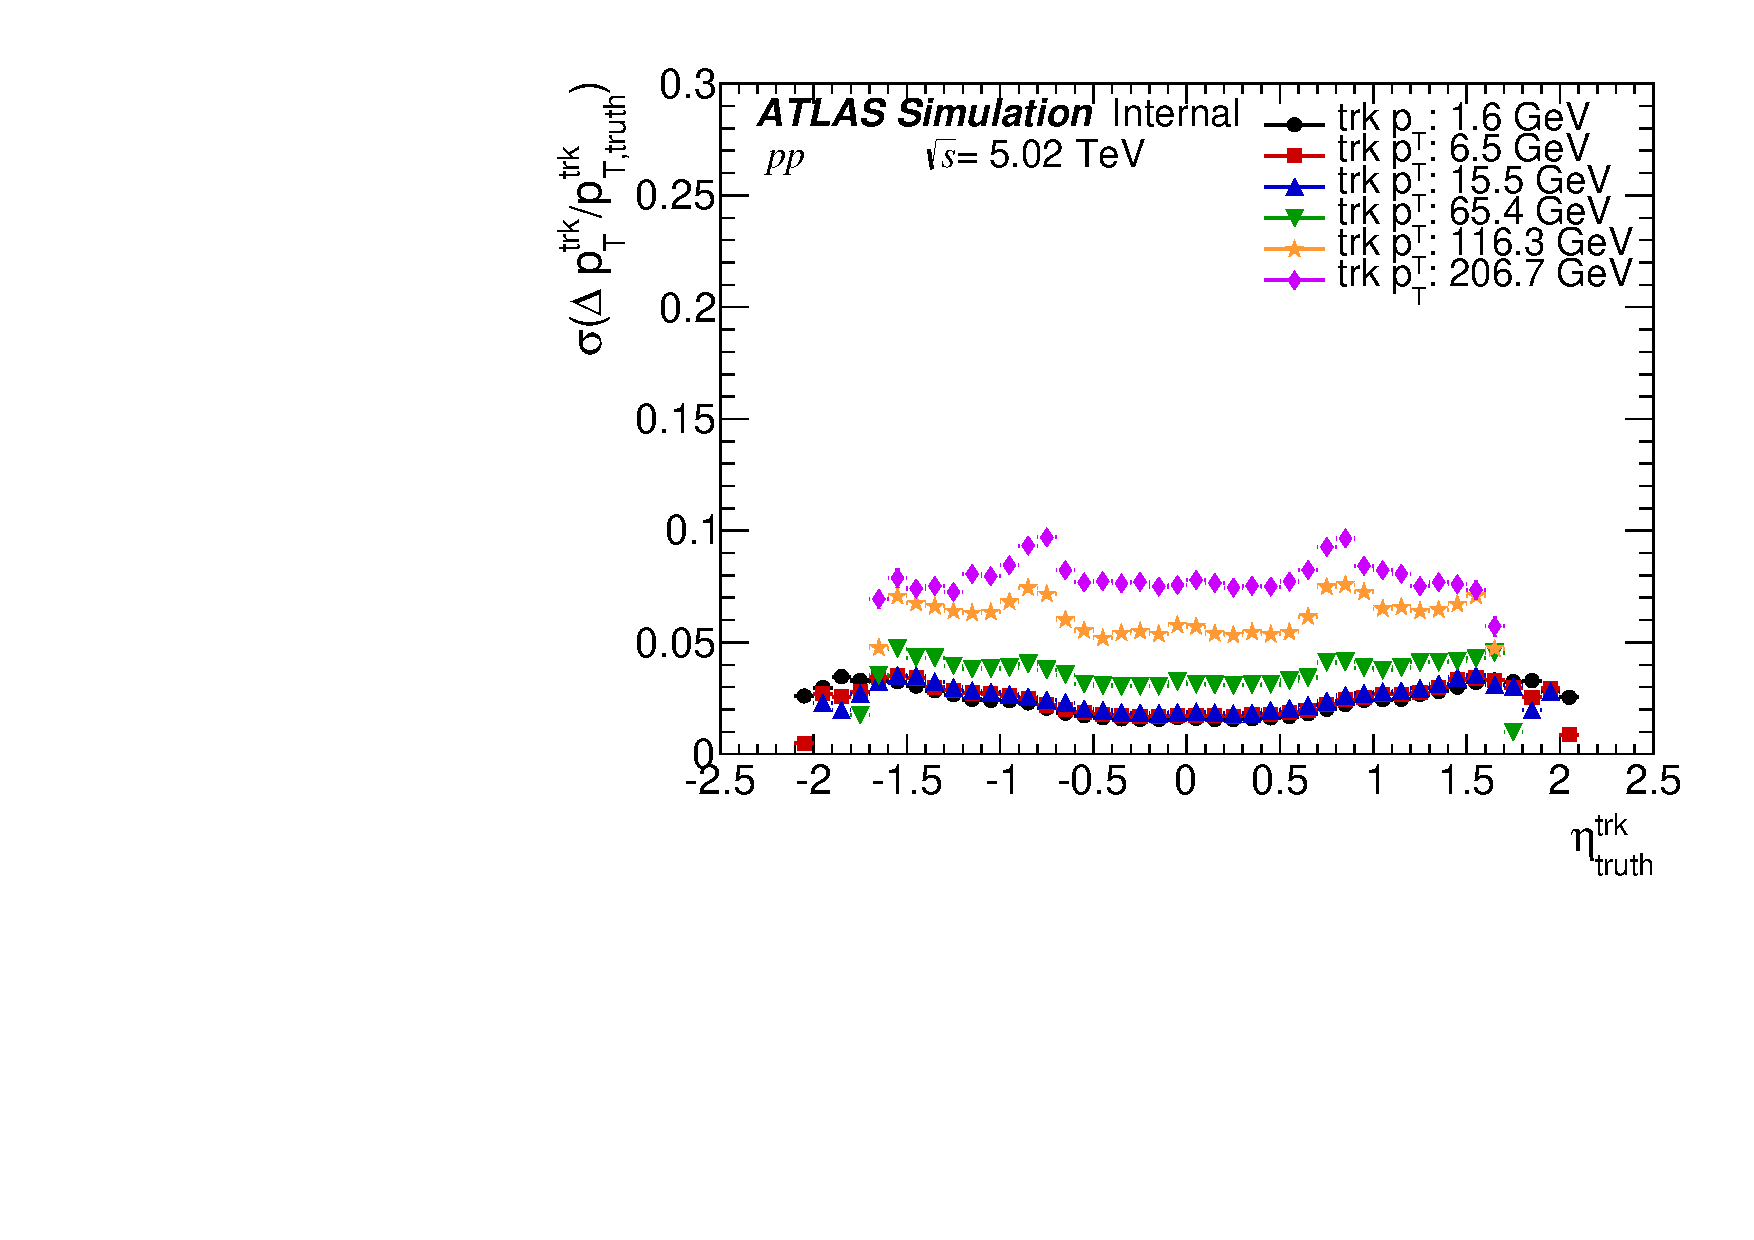
\includegraphics[width=0.45\textwidth]{figures/main/performance/resolution_v_eta_pp.pdf} \\ 
\end{tabular}}
\caption{(left) Comparison of the generated and reconstructed track \pt\ as a function of \etatrktruth\ for five track \pttrktruth\ selections.
(right) Track momentum resolution as a function of \etatrktruth\ for five \pttrktruth\ selections.
Both plots are for \pp\ MC.
All tracks shown in this plot have passed the 2015 default tracking cuts defined in this section.
The \pt\ in the legend corresponds to the bin centers in the following track \pt\ bins: 1.3 -- 1.8 GeV, 5.6 -- 7.5 GeV, 13.3 -- 17.7 GeV, 56.1 -- 74.8 GeV, 99.7 -- 132.9 GeV, \mbox{177.2 -- 236.2 GeV}.
Figure taken from Ref.~\cite{Sickles:2235420}.}
\label{fig:momres_pp}
\end{figure}



Figure~\ref{fig:ppcutflow_eta} presents the impact of individual tracking requirements in terms of the ratio of the number of tracks that pass given cut and the total number of reconstructed tracks in \pp\ MC.
This is shown as a function of track pseudorapidity in two different track \pT\ intervals and as a function of track \pT\ in two different pseudorapidity intervals.
The highest rejection for low \pT\ tracks is provided by the cut on $d_{0}$ pointing.
At high \pT\, the dominant effect is seen from the requirement on the number of silicon hits.
Similarly, Figure~\ref{fig:PbPbcutflow_eta} presents the impact of individual tracking requirements in \PbPb\ MC.
The difference between the impact of individual cuts can be attributed to a different setting of the tracking algorithm and to the overall increase of the track multiplicity as the number of rejected tracks does not linearly scale with the multiplicity that enters the denominator.


The primary particles\footnote{Primary particles are defined as particles with a mean lifetime $\tau>0.3\times 10^{-10}$ s either directly produced in \pp\ interactions or from subsequent decays of particles with a shorter lifetime.All other particles are considered to be secondary.}
used in this analysis have a mean lifetime \mbox{$\tau > 0.3 \times 10^{-10}$~s} and are either directly produced in \pp\ interactions or from subsequent decays of particles with a shorter lifetime.
They are required to have their barcode in the range $0 - 200000$.
Of these, particles with barcode $< 10000$ are coming from Pythia, while the remaining are from HIJING.
Particles with barcodes above 200000 are secondaries, and come from weak decays of $\Lambda$, $K_{S}$, $\Xi$, $\Sigma$, $\Omega$ and from particles created in interactions with the material.
Strange baryons are included: $\Sigma-$ (PDG ID 3112), $\Sigma+$ (PDG ID 3222), $\Xi-$ (PDG ID 3312), $\Omega-$ (PDG ID 3334).


\begin{figure}
\centering
\begin{tabular}{cc}
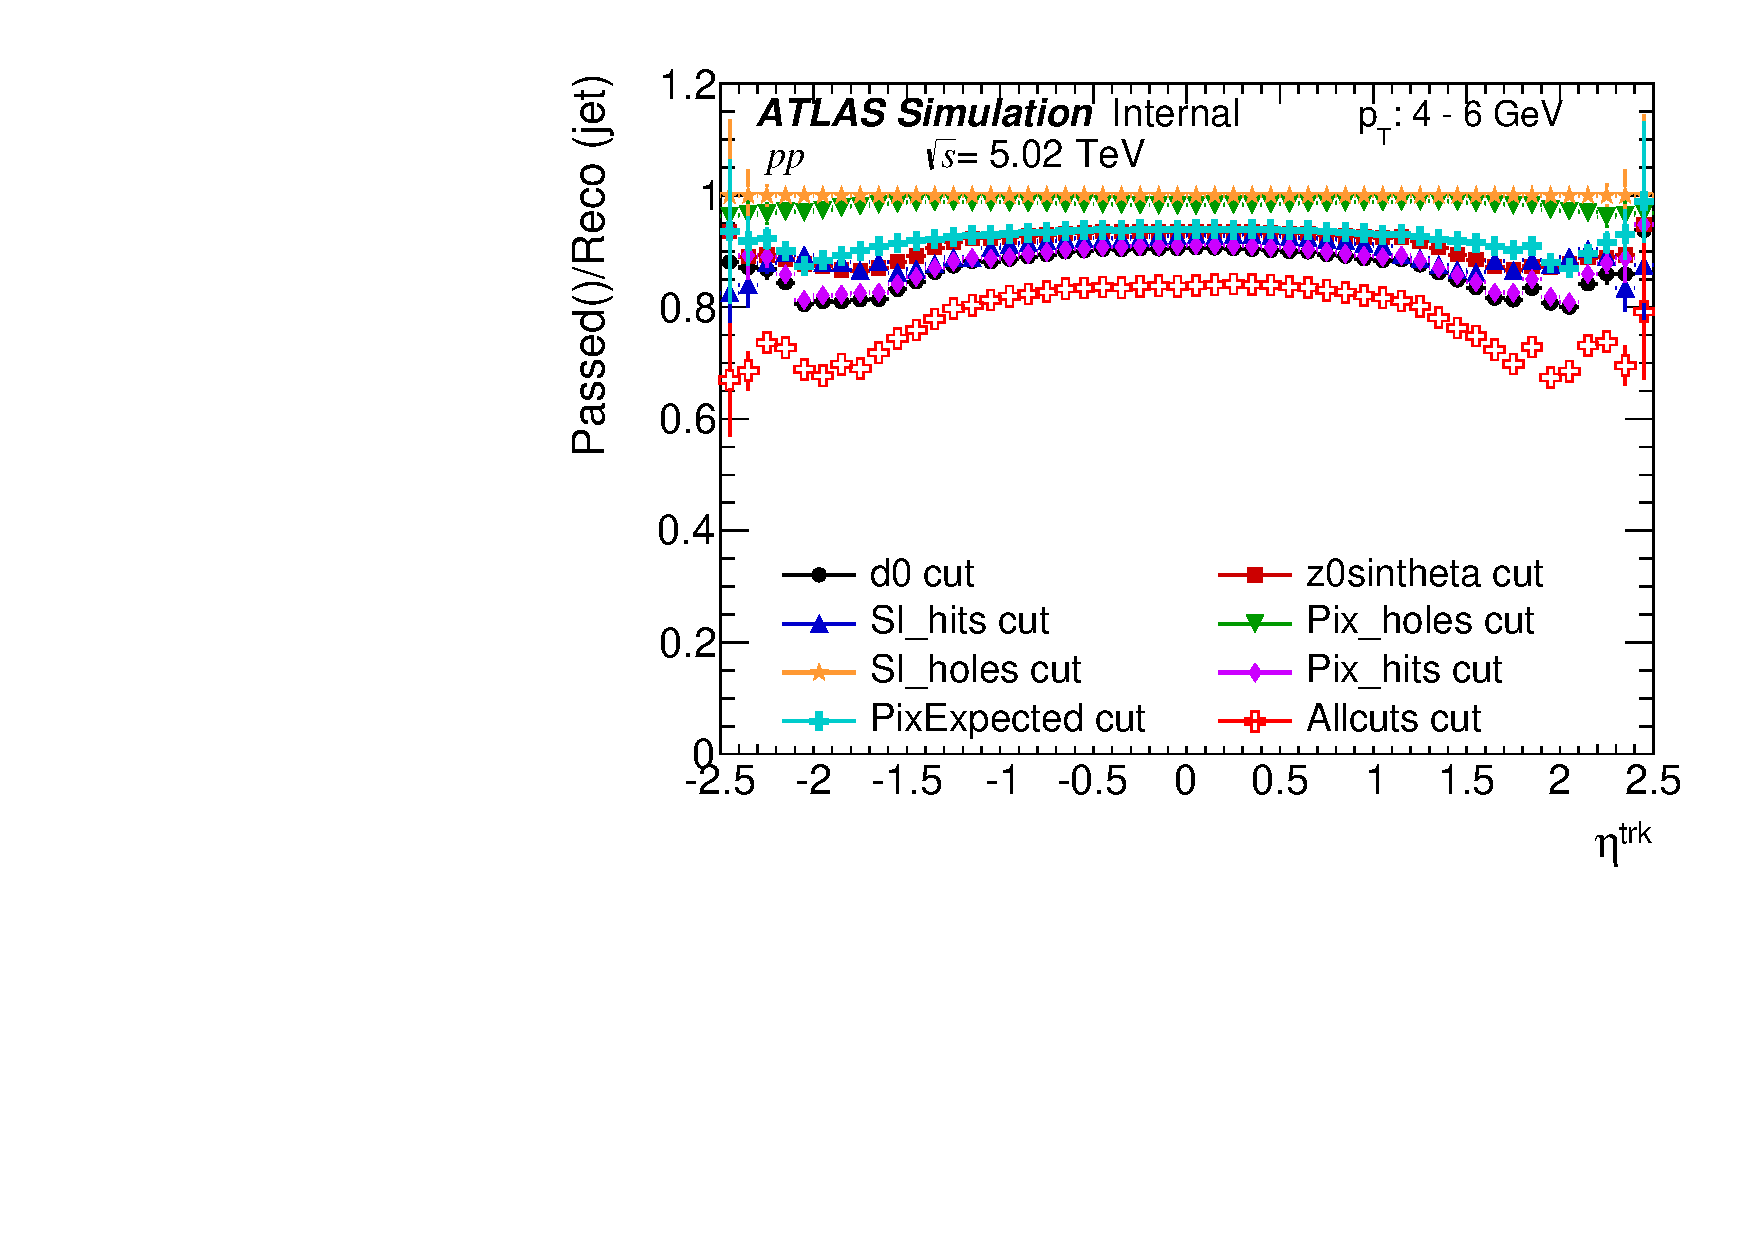
\includegraphics[width=0.45\textwidth]{figures/main/performance/cut_flow_RecoNorm_MC_pT_4_6_jet.pdf} &
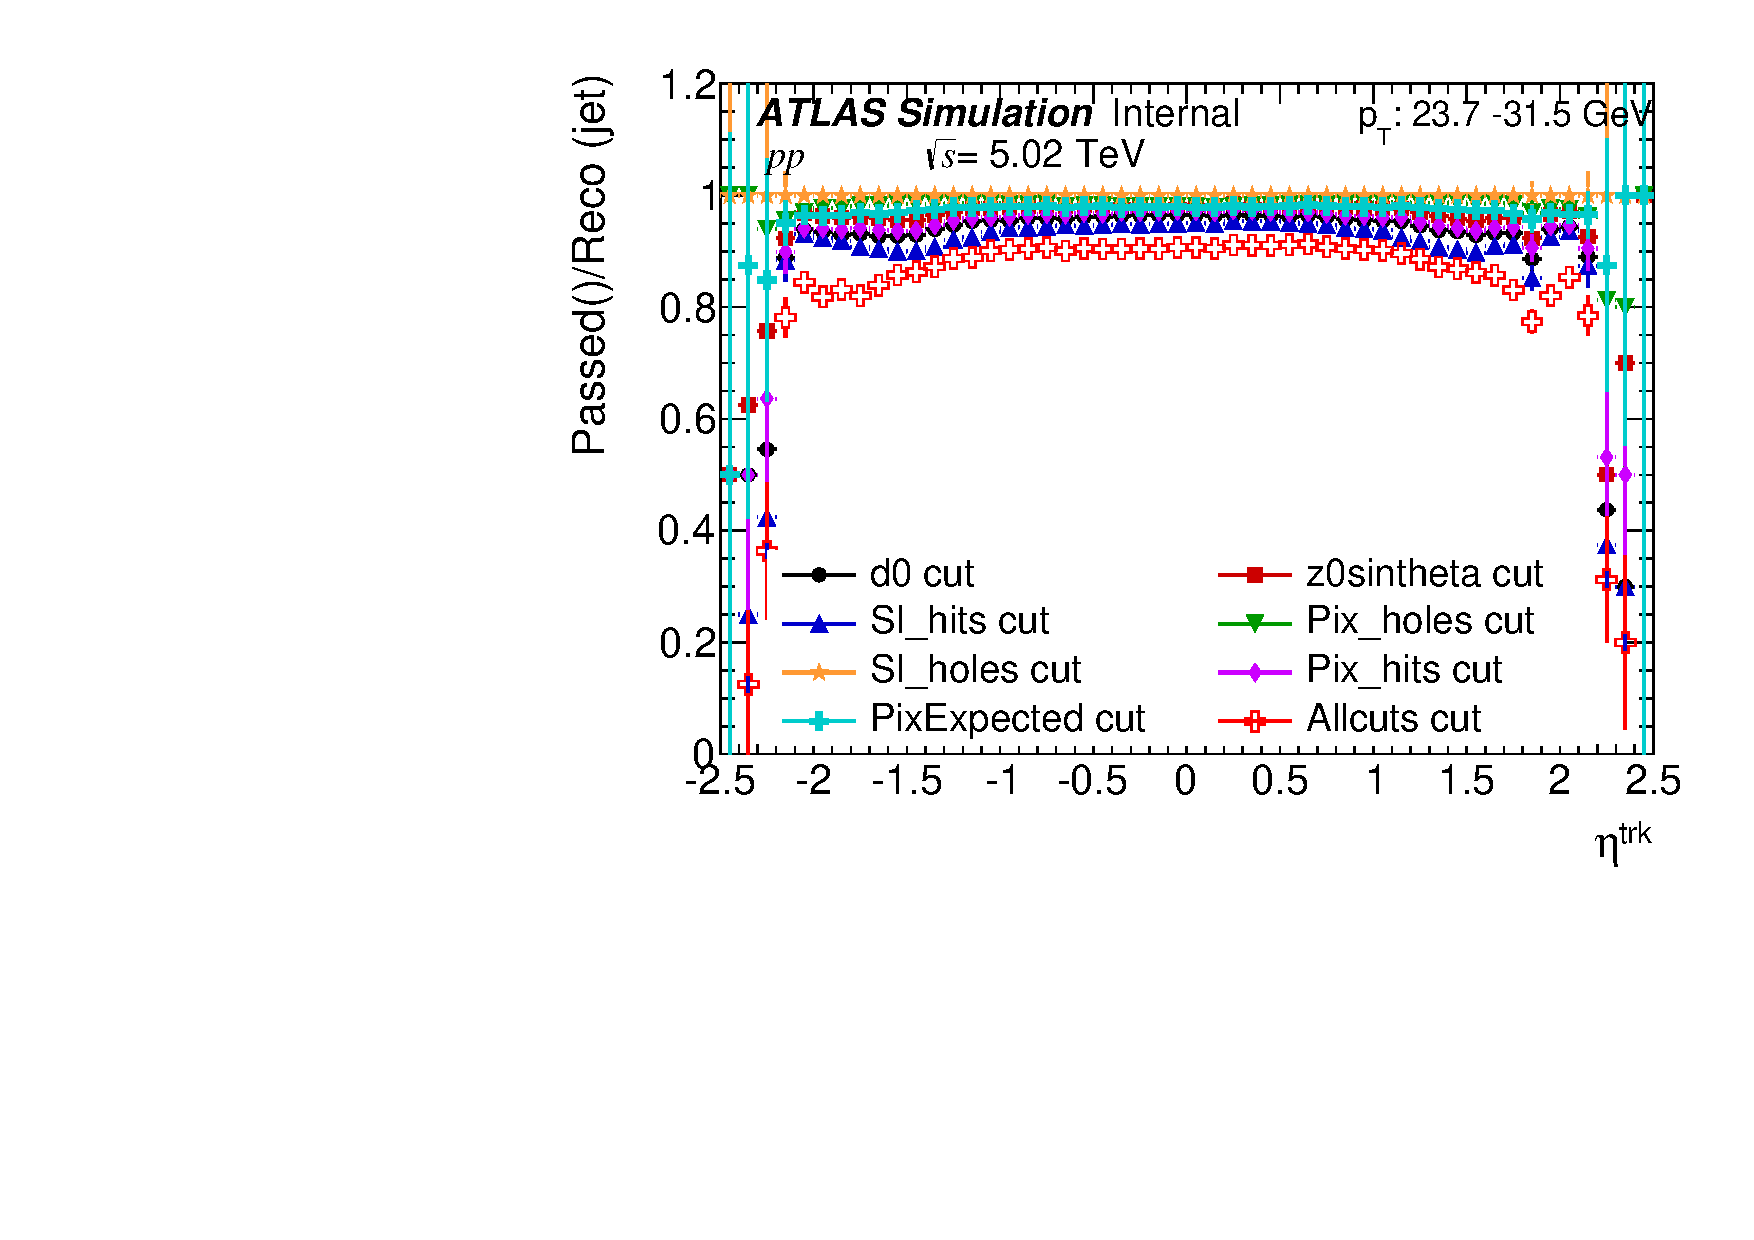
\includegraphics[width=0.45\textwidth]{figures/main/performance/cut_flow_RecoNorm_MC_pT_23p7_31p5_jet.pdf} \\
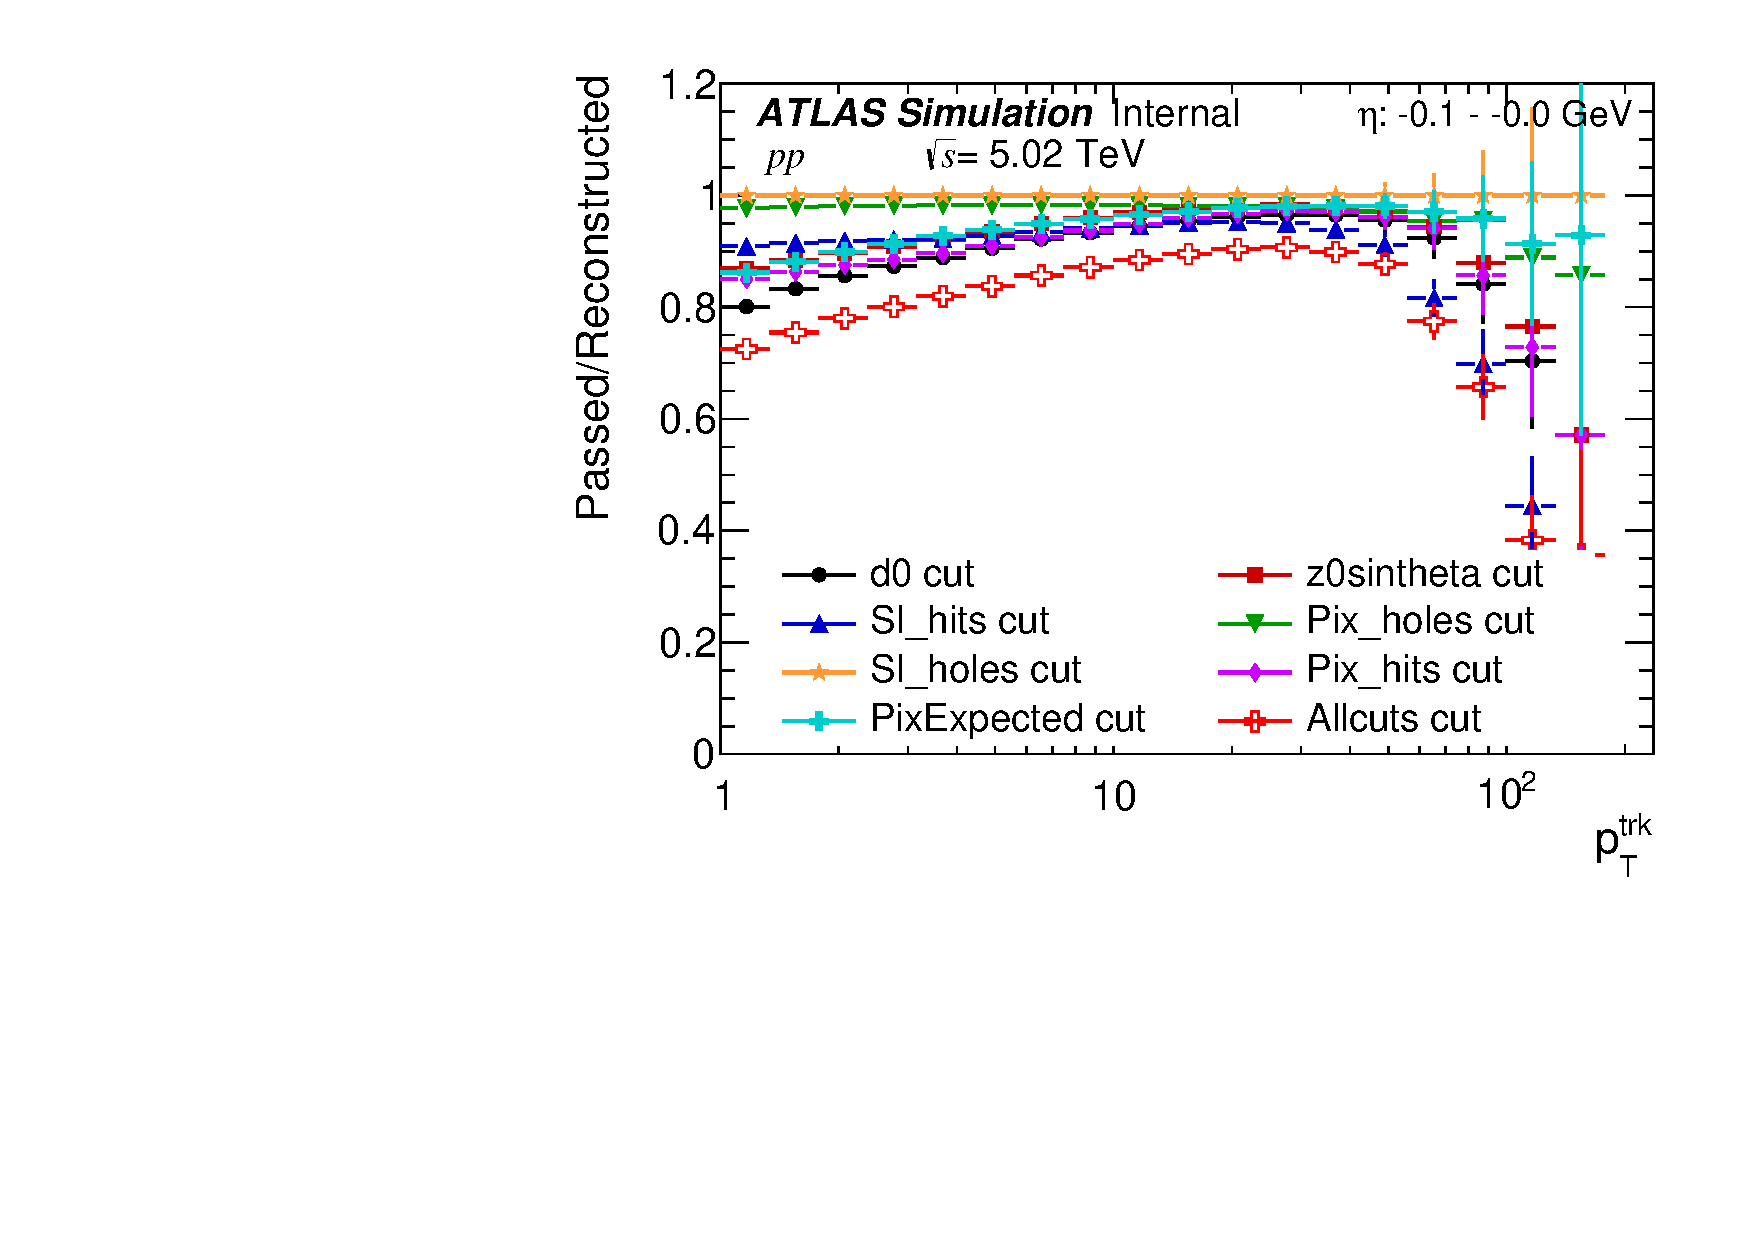
\includegraphics[width=0.45\textwidth]{figures/main/performance/cut_flow_RecoNorm_MC_eta_0p05_jet.pdf} &
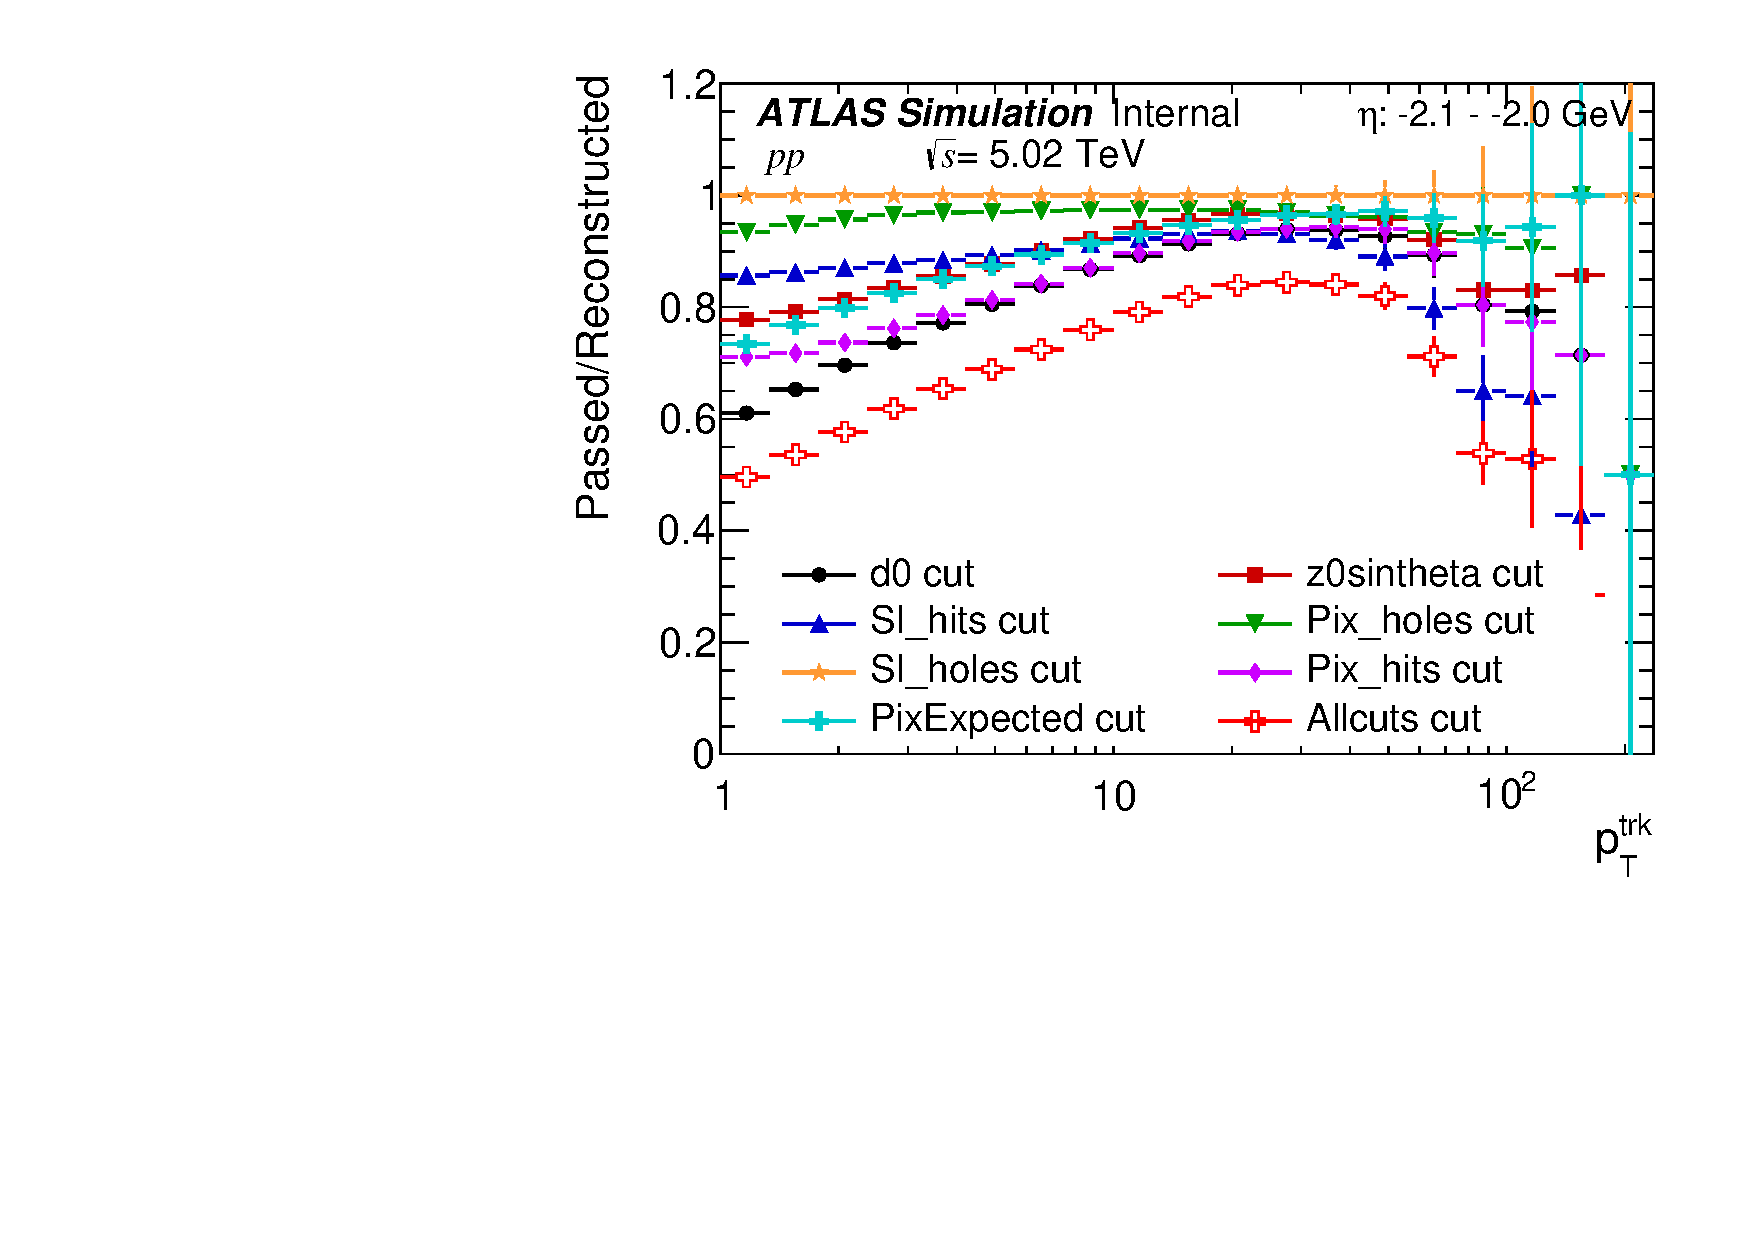
\includegraphics[width=0.45\textwidth]{figures/main/performance/cut_flow_RecoNorm_MC_eta_2p05_jet.pdf} \\
\end{tabular}
\caption{The impact of each cut applied individually in the \pp\ MC to the starting collection of tracks, as a function of
\etatrk (top) for 1.3~$< \pttrk<$~4.6~GeV (left) and for 23.7~$<\pttrk<$~31.5~GeV and as a function of track \pT\ for two different pseudorapidity intervals (bottom).
The final combination of all cuts is shown as well.
Figure taken from Ref.~\cite{Sickles:2235420}.}
\label{fig:ppcutflow_eta}
\end{figure}

\begin{figure}
\centering
\begin{tabular}{cc}
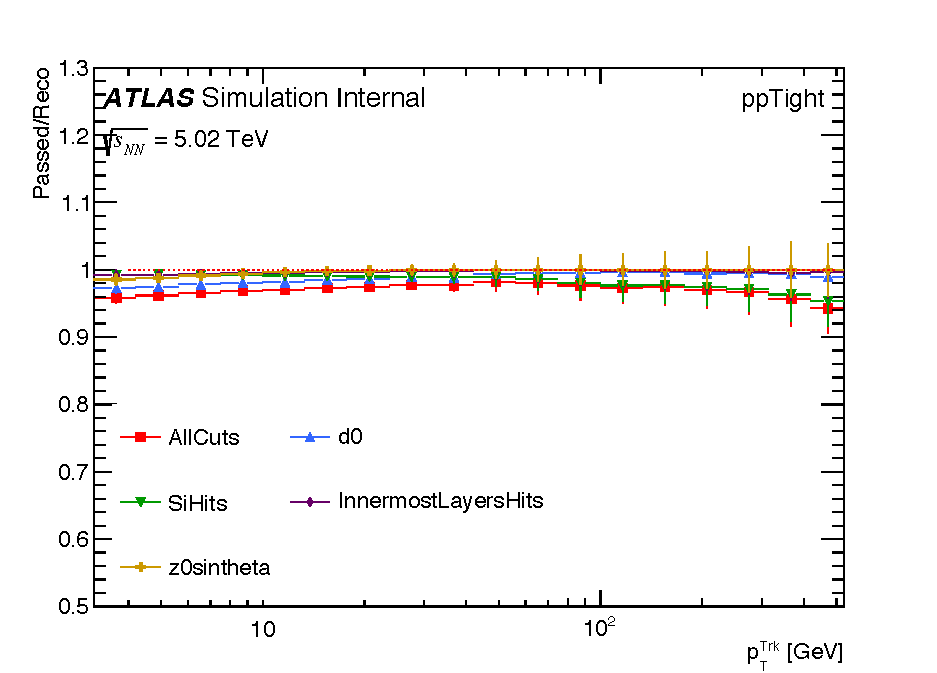
\includegraphics[width=0.45\textwidth]{figures/main/performance/PbPb_cutflow_pptight.pdf} &
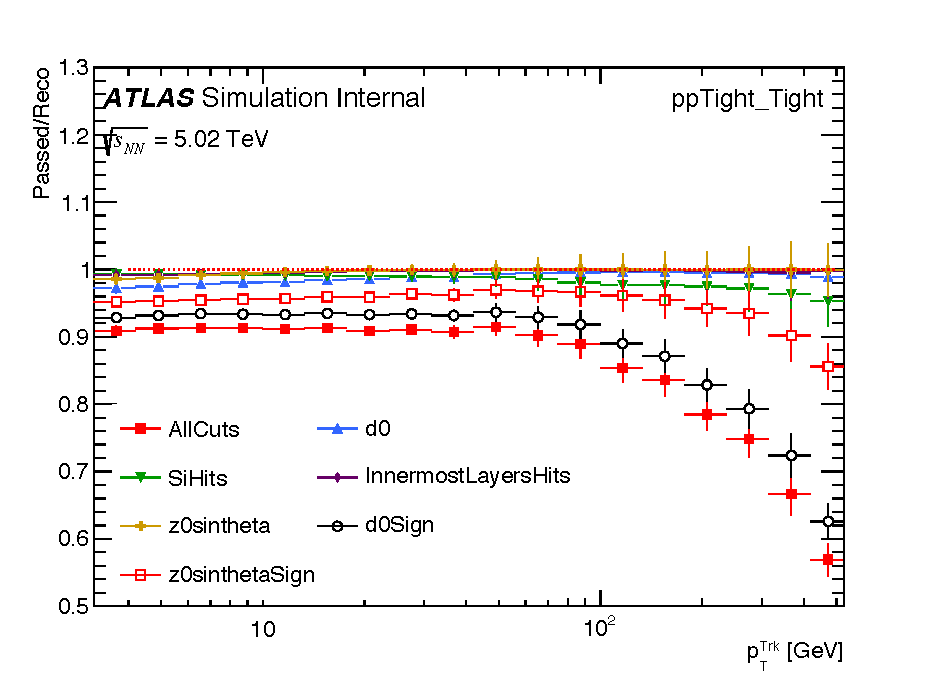
\includegraphics[width=0.45\textwidth]{figures/main/performance/PbPb_cutflow_pptight_tight.pdf} \\
\end{tabular}
\caption{The impact of each cut applied individually in the \PbPb\ MC 
to the starting collection of tracks, as a function of the track \pT\ inclusive in collision centrality for the default and the tight set of tracking requirements.
The final combination of all cuts
is shown as well.}
\label{fig:PbPbcutflow_eta}
\end{figure}



%%%%%%%%%%%%%%%%%%%%%%%%%%%%%%
\subsection{Track momentum correction}
\label{Sec:Trackmomentumcorrection}
Specific corrections are needed for track momentum in 5.02~TeV \pp\ and \PbPb\ data to account for a miss-alignment introduced in the track reconstruction.
The sign charge dependent momentum scale shift was observed in \pp\ data when the transverse momentum of muons reconstructed using muon spectrometer was compared to the transverse momentum of muons from the inner detector.
The difference as a function of muon momentum in \pbpb\ data can be seen in Figure~\ref{fig:ChMomentumScale}.
The correction to track \pt\ as a function of track $\eta$ and track $\phi$ is applied through sagitta bias maps introduced in Ref.~\cite{TrackingRec}.

\begin{figure}[h]
\centering
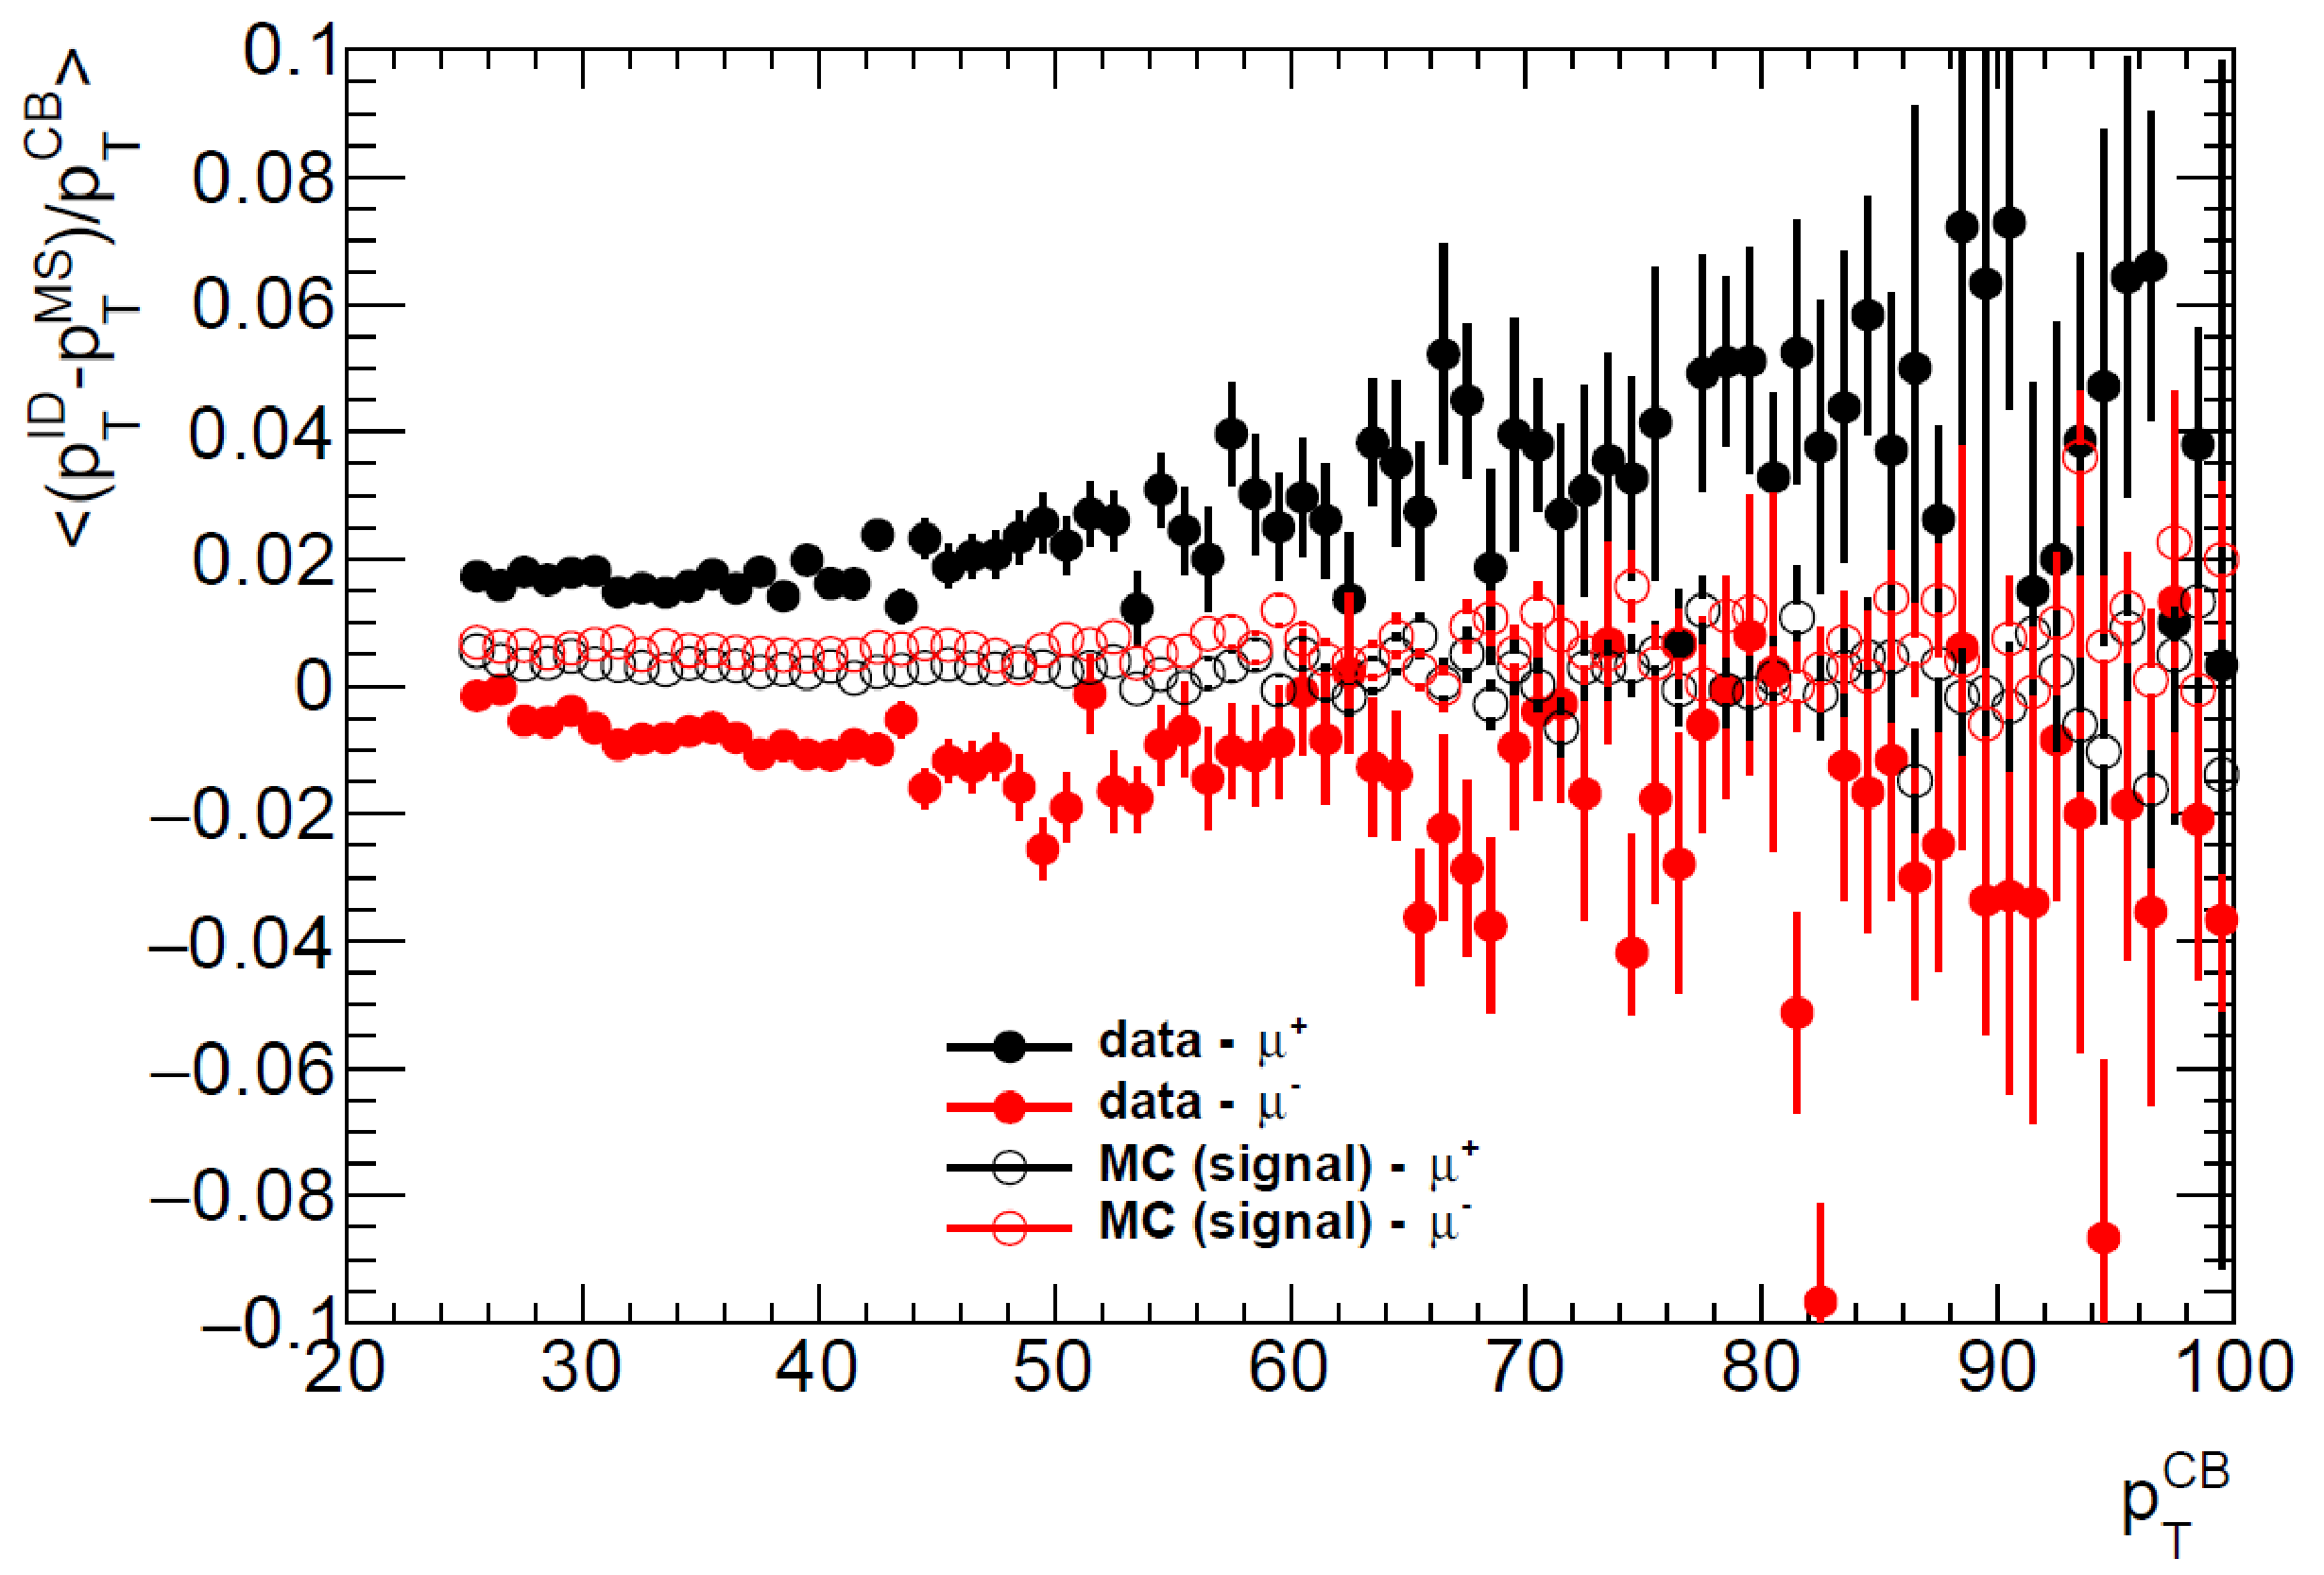
\includegraphics[width=0.55\textwidth]{figures/main/corrections/MuonPerf.pdf}
\caption{Comparisons of track momentum scale of positive and negative muons reconstructed using muon spectrometer and inner detector.
The muon traverse momentum evaluated from muon spectrometer (MC) is compared by that evaluated using the inner detector (ID) and the relative scale is normalized by the momentum that uses both detectors.
Taken from \cite{Bold:2194917}.}
\label{fig:ChMomentumScale}
\end{figure}


%%%%%%%%%%%%%%%%%%%%%%%%%%%%%%
\subsection{Track reconstruction efficiency}
\label{sec:trackreco}

The tracking reconstruction efficiency is defined as the ratio between the number of primary truth charged particles that are reconstructed and the total number of primary truth charged particles in the given \pt\ and $\eta$ bin.
It is evaluated using MC tracks, where tracks are required to pass all the tracking cuts imposed on the data.

Matching between the reconstructed and the truth track is done via a cut on \mcprob.
This is defined as the probability that a reconstructed track matched to a truth track actually was a truth track.
It is calculated as:

\begin{align}
\mcprob = \frac{10N^{\mathrm{common}}_{\mathrm{pix}} + 5N^{\mathrm{common}}_{\mathrm{SCT}} + N^{\mathrm{common}}_{\mathrm{TRT}}}{10N^{\mathrm{track}}_{\mathrm{pix}} + 5 N^{\mathrm{track}}_{\mathrm{SCT}} + N^{\mathrm{track}}_{\mathrm{TRT}}}
\end{align}
where $N^{\mathrm{common}}_X$  are the number of hits in detector $X$ in common between the truth and reconstructed track.
$N^{\mathrm{track}}_X$ is the number of total hits in the reconstructed track.

Tracks with $\mcprob > 0.3$ are associated with the truth track and those with a lower value are not and are classified as fake tracks.
The choice of $\mcprob = 0.3$ is based on the recommendation from the ATLAS tracking group and was used in~\cite{201865}.
The sensitivity of the measurement on the value of the \mcprob\ cut is included in the systematic uncertainties.

In MC samples, the ``track barcode'' classifies reconstructed tracks to different classes based on the origin (primary, secondary, pileup, beam halo, fake).
We require $0 < \mathrm{barcode} < 200000$ in evaluation of the tracking efficiency to remove pileup, beam halo, secondary particles, and fake particles.
Reconstructed tracks that do not have a matched truth track with given \mcprob\ are labeled all together as fake tracks.
The tracking cuts need to provide both good efficiency for generator level tracks and to adequately reject fakes.

\begin{figure}
\centering
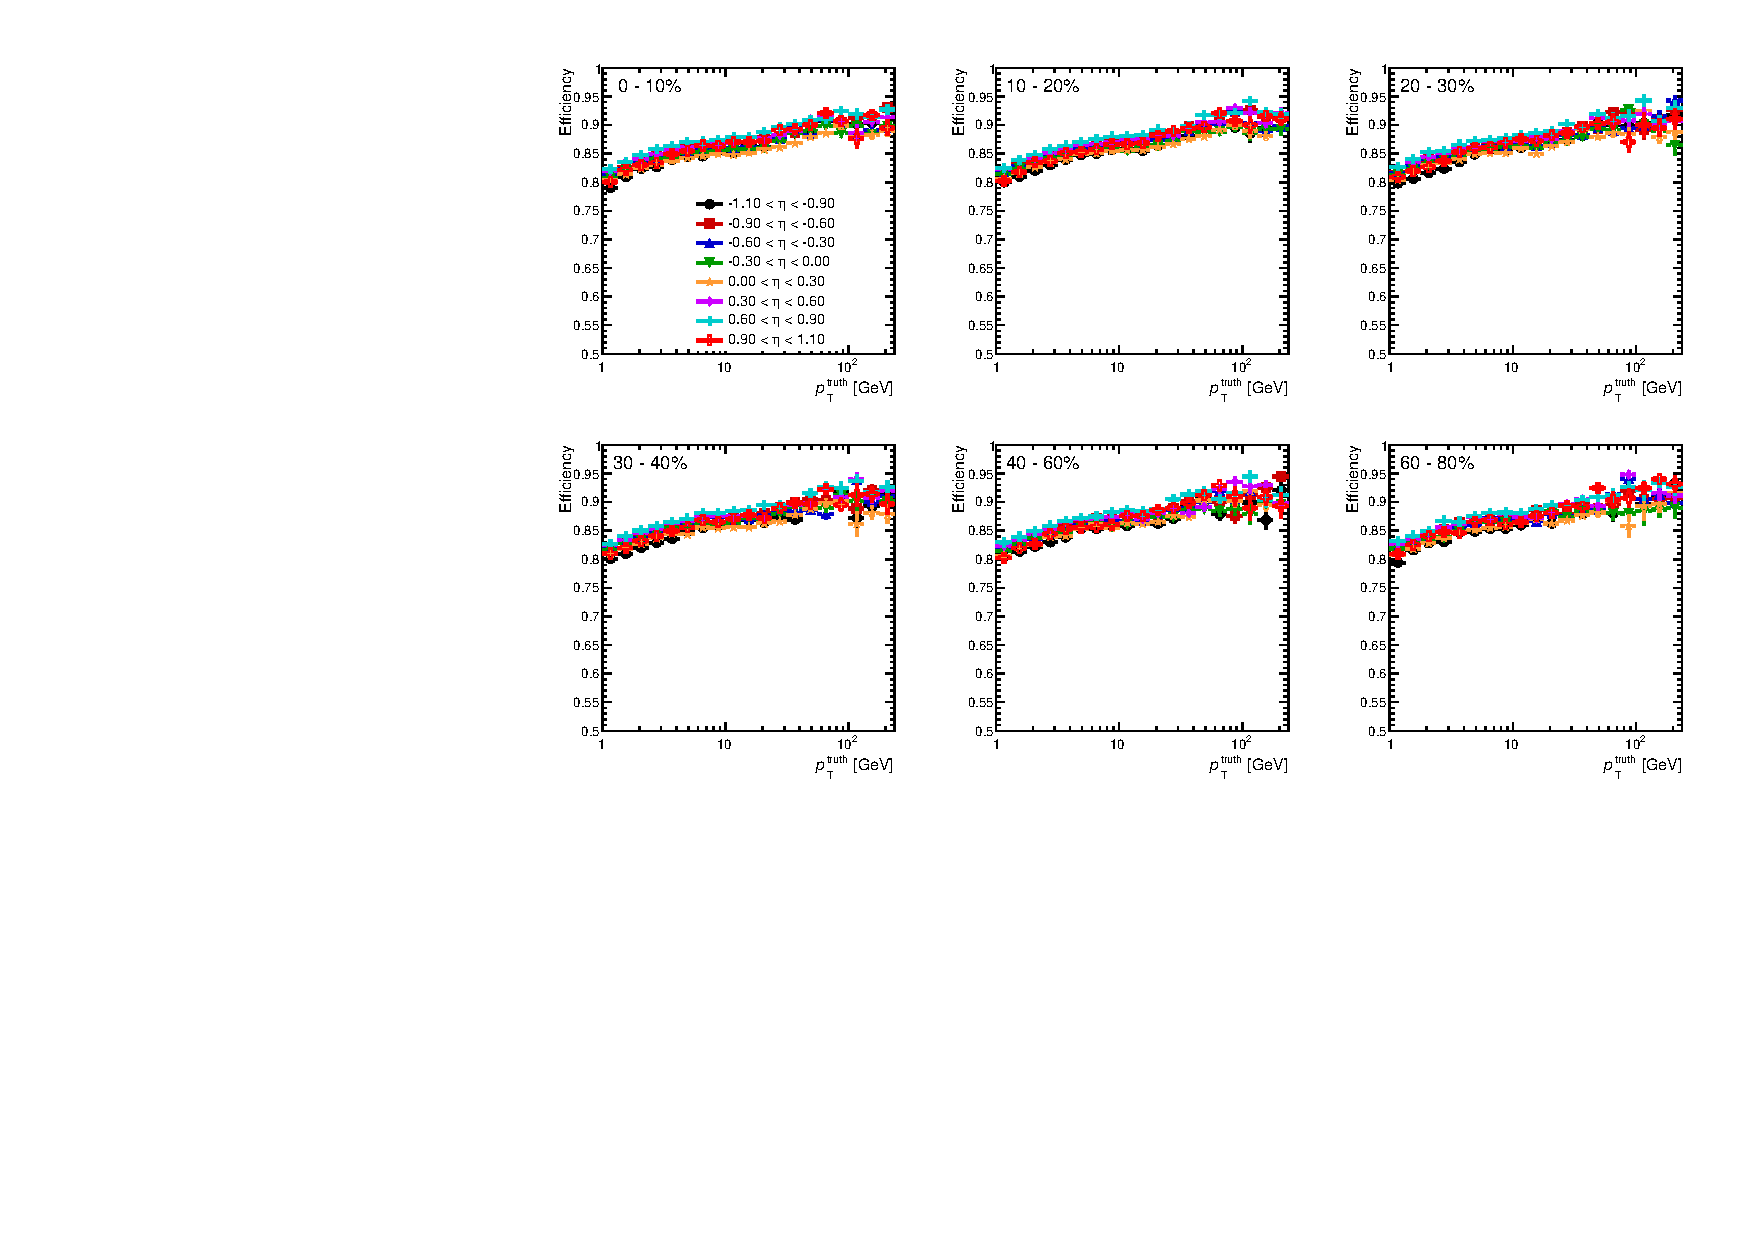
\includegraphics[width=0.7\textwidth]{figures/main/corrections/eff_cent_trketa_PbPb_ppTight.pdf}
\caption{Efficiency for reconstructing tracks evaluated using the default tracking selections in different track $\eta$ bins in the \pbpb\ MC overlay samples.
Each panel is a different centrality bin.}
\label{fig:pbpbeffdefault_final}
\end{figure}

\begin{figure}
\centering
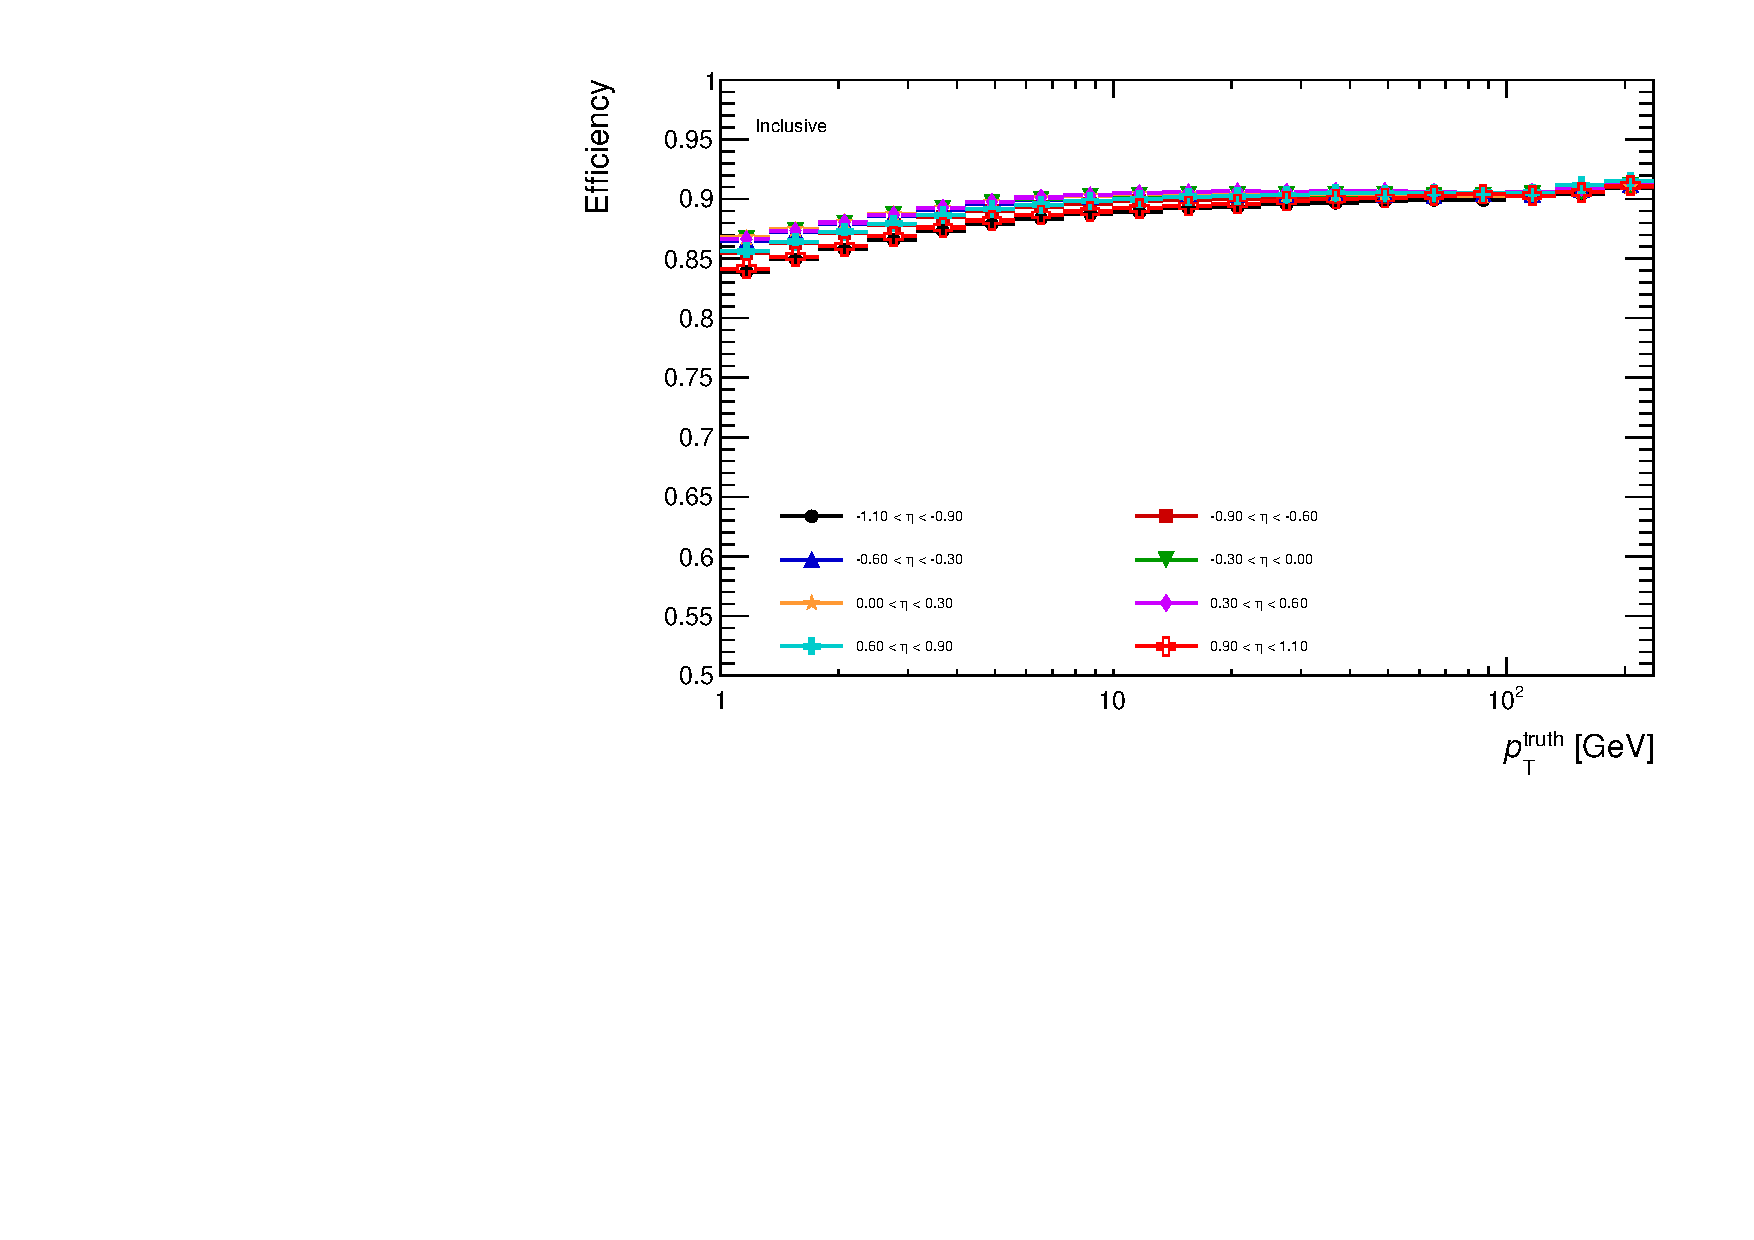
\includegraphics[width=0.45\textwidth]{figures/main/corrections/eff_cent_trketa_pp_ppTight.pdf}
\caption{Efficiency for reconstructing tracks evaluated using the default tracking selections in different track $\eta$ bins in the \pp\ MC samples.}
\label{fig:ppeffdefault_final}
\end{figure}

The final efficiency corrections applied were determined and applied as a function track \pt\ and track $\eta$, and can be seen in Figures~\ref{fig:pbpbeffdefault_final}-\ref{fig:ppeffdefault_final} for \pp\ and \PbPb\ collisions.
No significant dependence on the collision centrality is observed.
The efficiency exhibits a small, but monotonic increase with the track \pt.
Only a small variation with the track $\eta$ is observed in the region $|\eta|<1.1$.
The efficiency correction is applied on a track-by-track basis, assuming $\pttrk = \pTtrue$.
While that assumption is not strictly valid, the efficiency varies sufficiently slowly with $\pTtrue$ that the error introduced by this assumption is negligible, up to 1\%.
The tracking efficiency determined in Ref.~\cite{PhysRevC.98.024908} was not seen to be dependent on \ptjet\ for $\pttrk \lesssim 40$ GeV as can be seen in Figures~\ref{fig:pbpbeffdefaultjetpt_y0}-\ref{fig:ppeffdefaultjetpt}.
The small depletion of the efficiency for tracks with $\pt \sim 10-40$~GeV was attributed to the convolution of how jet fragments and with the performance of the track reconstruction in the dense core of the jet~\cite{PhysRevC.98.024908}.


\begin{figure}
\centering
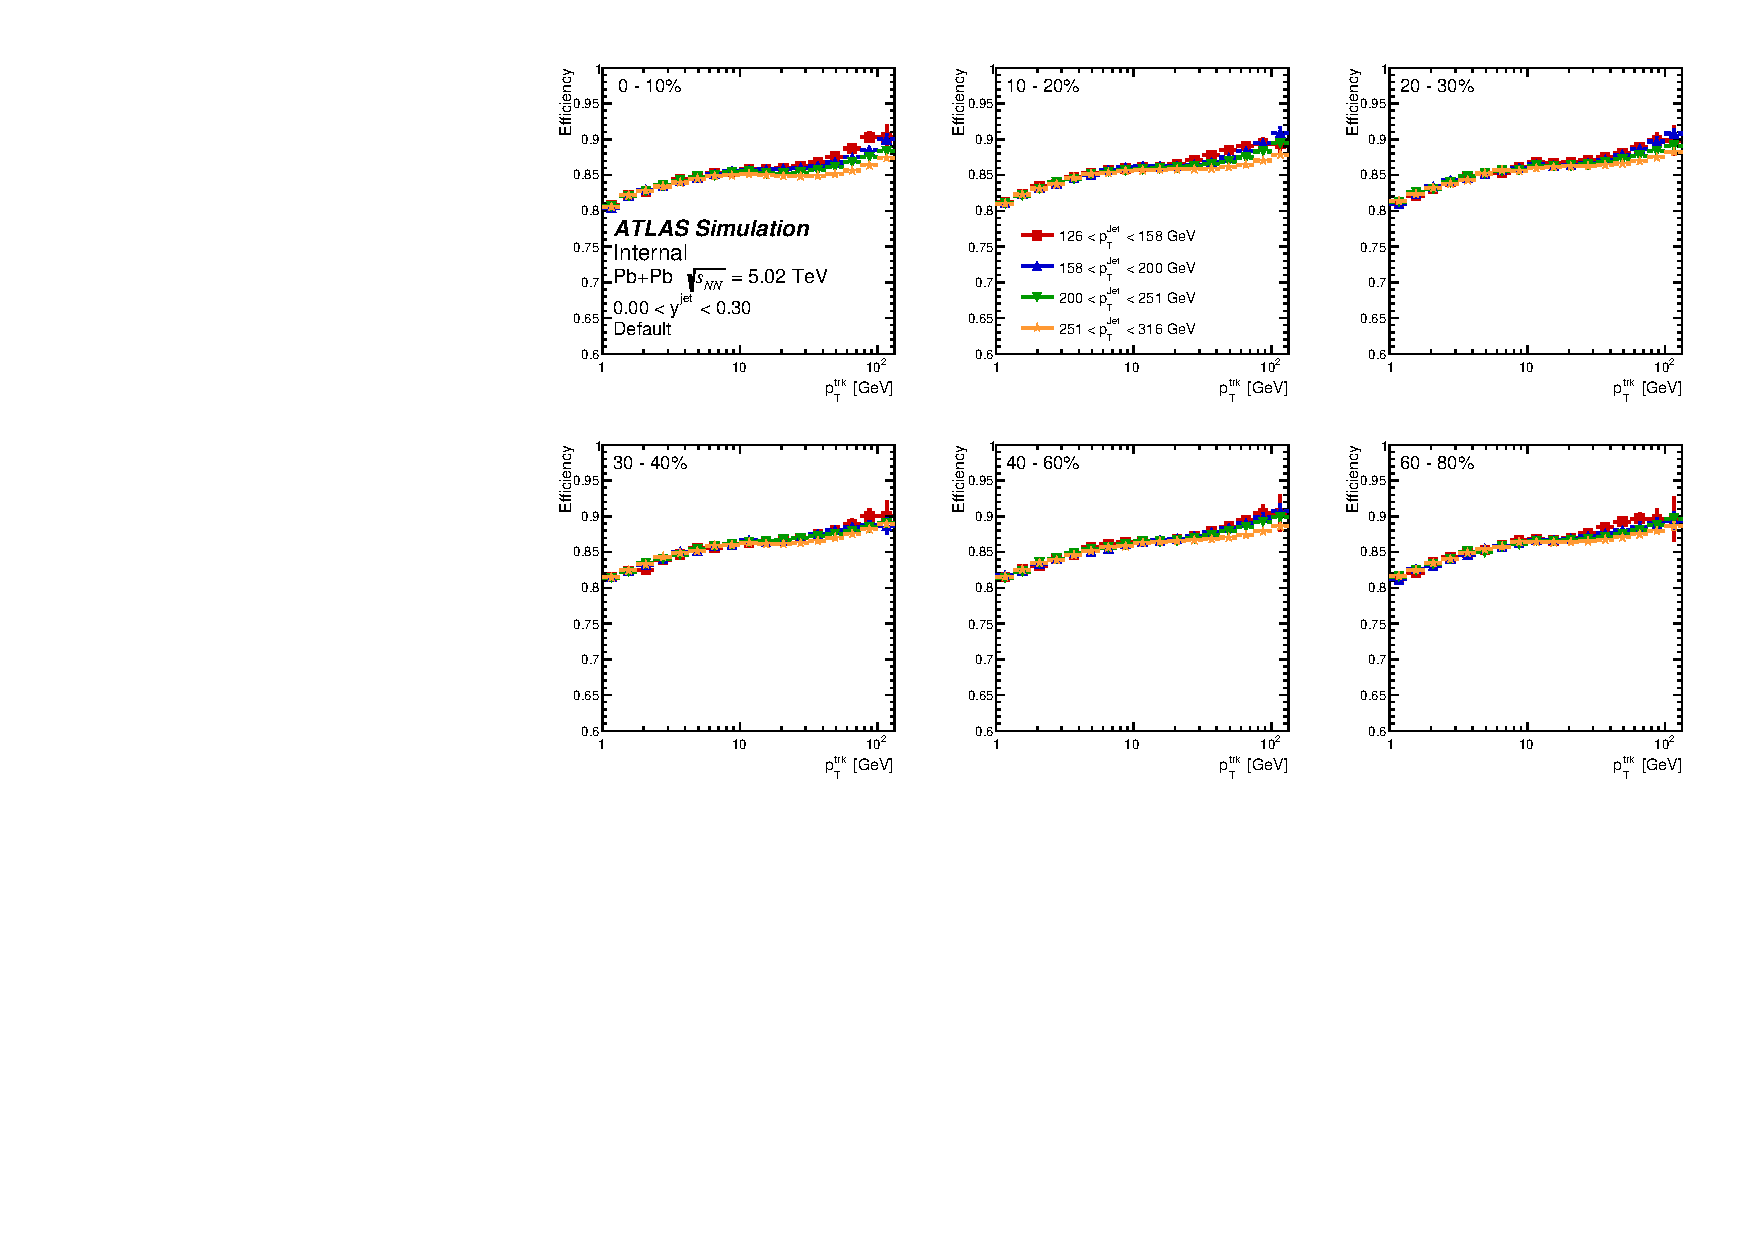
\includegraphics[width=0.7\textwidth]{figures/main/corrections/eff_centrality_jetpt_jety0_ppTight.pdf}
\caption{Efficiency for reconstructing tracks evaluated using the default tracking selections in different jet \pT\ bins and jet rapidity interval $|y|<0.3$ in the \pbpb\ MC overlay samples.
Each panel is a different centrality bin.}
\label{fig:pbpbeffdefaultjetpt_y0}
\end{figure}

\begin{figure}
\centering
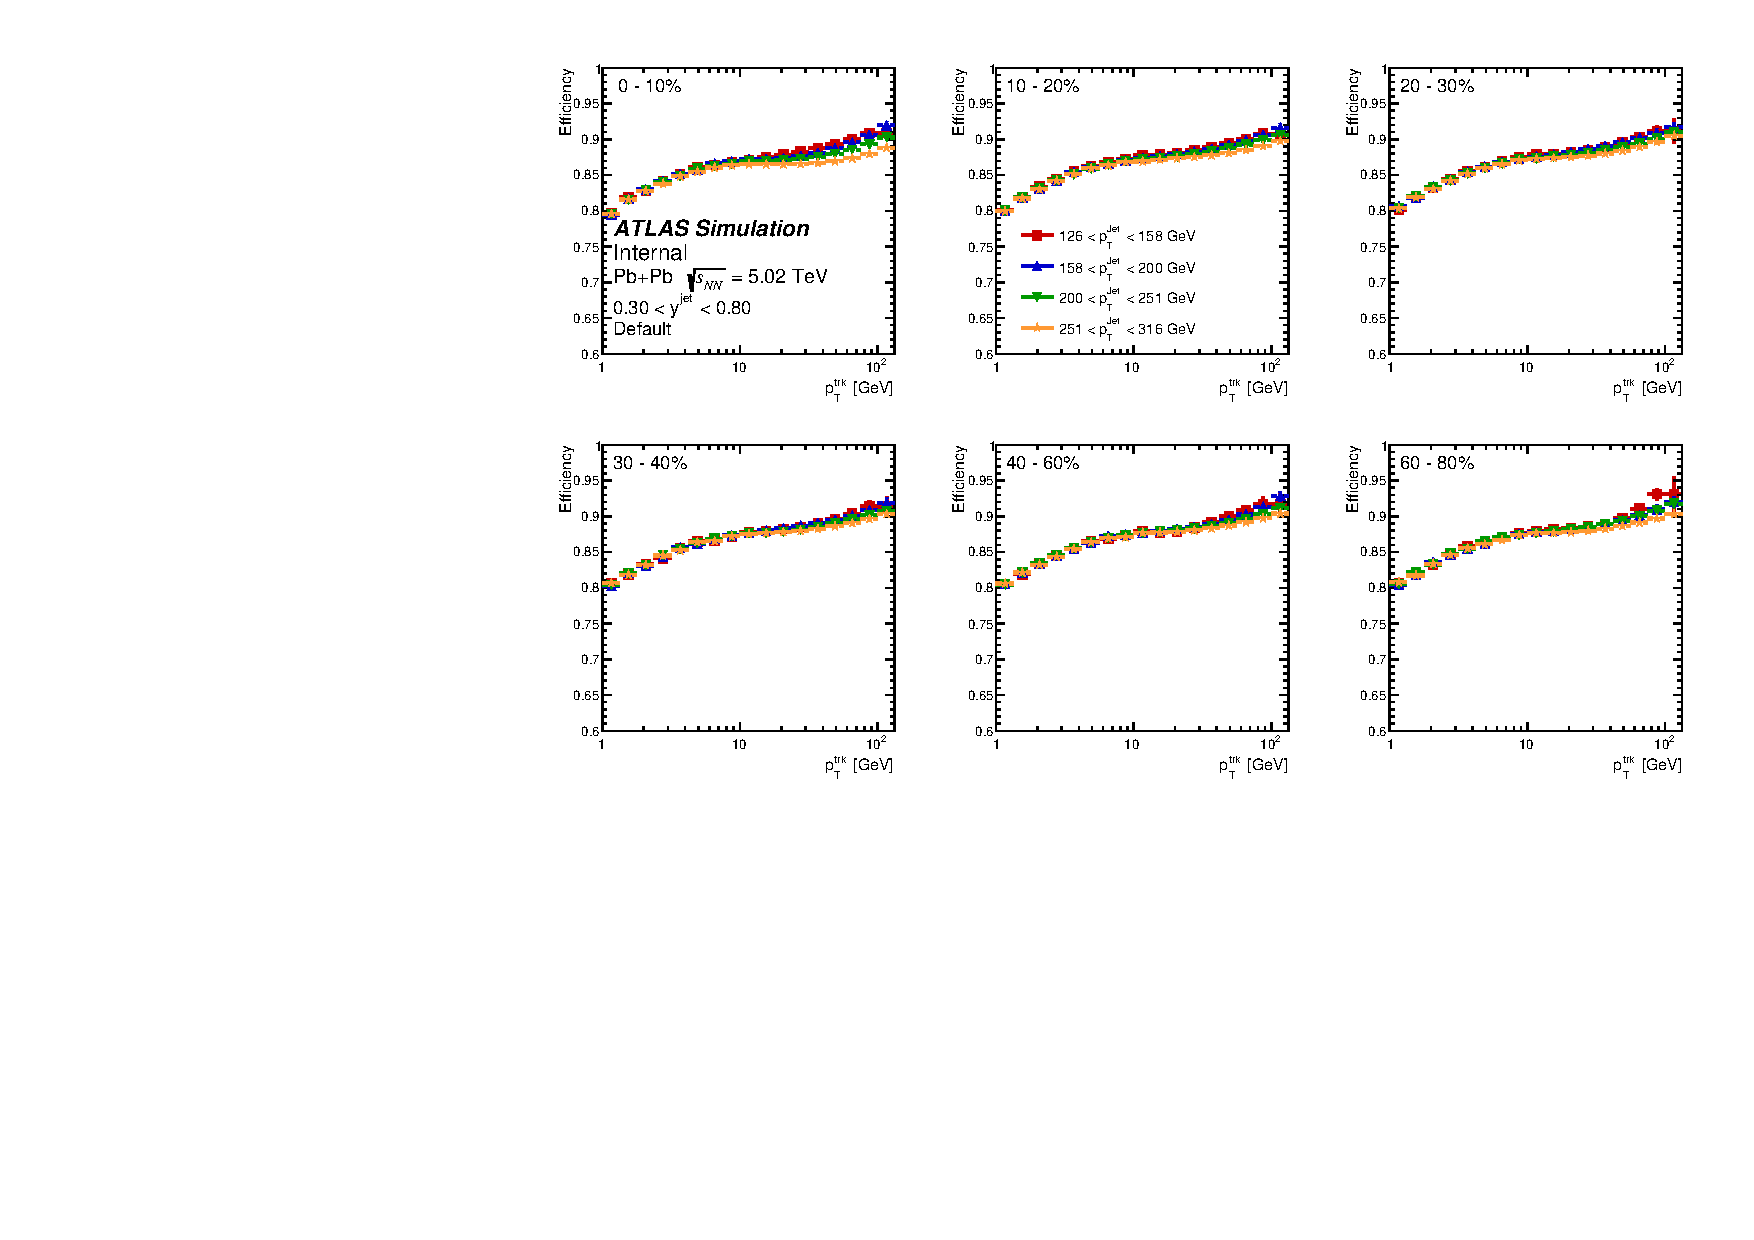
\includegraphics[width=0.7\textwidth]{figures/main/corrections/eff_centrality_jetpt_jety1_ppTight.pdf}
\caption{Efficiency for reconstructing tracks evaluated using the default tracking selections in different jet \pT\ bins and jet rapidity interval $0.3<|y|<0.8$ in the \pbpb\ MC overlay samples.
Each panel is a different centrality bin..}
\label{fig:pbpbeffdefaultjetpt_y1}
\end{figure}

\begin{figure}
\centering
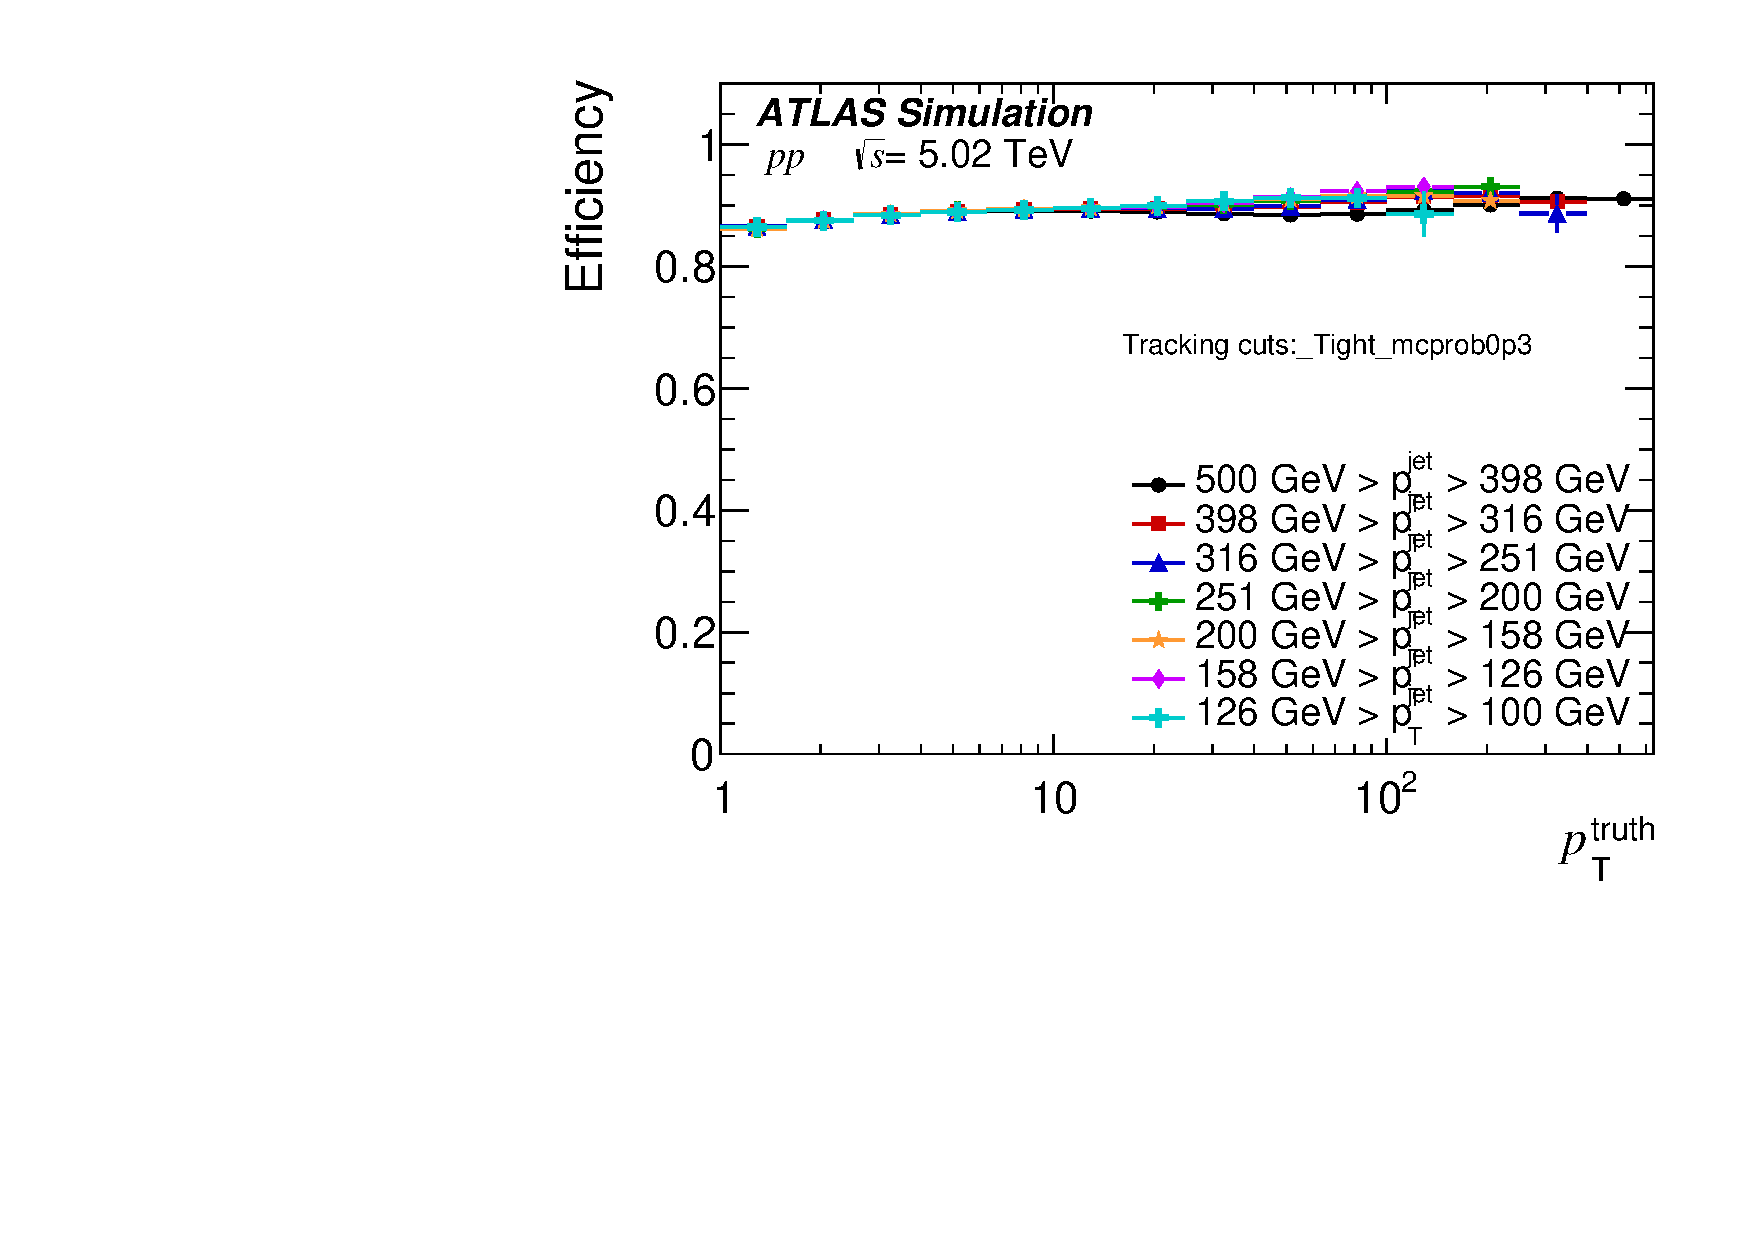
\includegraphics[width=0.45\textwidth]{figures/main/corrections/Trk_eff_v_pt_r005f_Tight_mcprob0p3_CX_Injet_0p0_0p3_pp_5p02.pdf}
\caption{Efficiency for reconstructing tracks evaluated using the default tracking selections in different jet \pT\ bins, in the \pp\ MC samples.}
\label{fig:ppeffdefaultjetpt}
\end{figure}

%%%%%%%%%%%%%%%%%%%%%%%%%%%%%%
\subsection{Fake rates}
\label{sec:fakerates}
Reconstructed tracks that cannot be matched to a primary particle in the MC samples or are matched to a secondary particle are considered to be ``fake'' tracks.
The rate of these tracks was evaluated and extensively studied in Ref.~\cite{PhysRevC.98.024908} in the \pp, \pbpb\ HIJING MC, and in \pbpb\ MC overlay samples.
The MC overlay sample is used to crosscheck the fake rate at higher \pt, but is not used for any corrections.
It was shown that as the \pttrk\ approaches the  \ptjet\ the fraction of fake tracks increases due to the steeply falling spectra of generator level tracks.
Figures~\ref{fig:fakeratepp} and \ref{fig:fakeratepbpb} show the fraction of tracks that are identified as fakes, secondaries, or part of UE in case of \PbPb\ collisions as a function of \pttrk\ for selections in \ptjet in \pp\ and \pbpb\ collisions, respectively.
The rate decreases with \pttrk\ up to approximately 10~GeV and then remains constant until \pttrk\ approaches \ptjet\ where the rate increases again.
In \pbpb\ collisions, the ``fake'' rate also includes tracks which are from the underlying event from the real collisions into which the jet is overlaid.
The rate of these underlying event tracks increases with decreasing \pttrk\ and increasing collision centrality.
The contribution from UE is negligible for tracks with \pT\ above 10 GeV as no centrality dependence is seen.
The Figure~\ref{fig:fakeratepbpb} excludes the very low \pT\ region where the distribution would be completely dominated by the UE.
The size of the UE is then presented further in Figure~\ref{fig:UEimpact}.
To separate the contribution of UE tracks (see section~\ref{sec:cuts_UE}) from the fake tracks in \PbPb\ collisions and cross-check the centrality dependence of the fake rate, 200,000 MB \PbPb\ fully reconstructed HIJING MC~\cite{Wang:1991hta} events were used.
The HIJING MC generator is capable of simulating global properties of HI collisions.
The estimated fake rate of tracks associated with jets with $\pT>40$ GeV is at the level of 1\% and it exhibits similar behavior as observed in Figure~\ref{fig:fakeratepbpb}.
No significant dependence of the fake rate on the collision centrality was found~\cite{PhysRevC.98.024908}.

\begin{figure}
\centering
\begin{tabular}{cc}
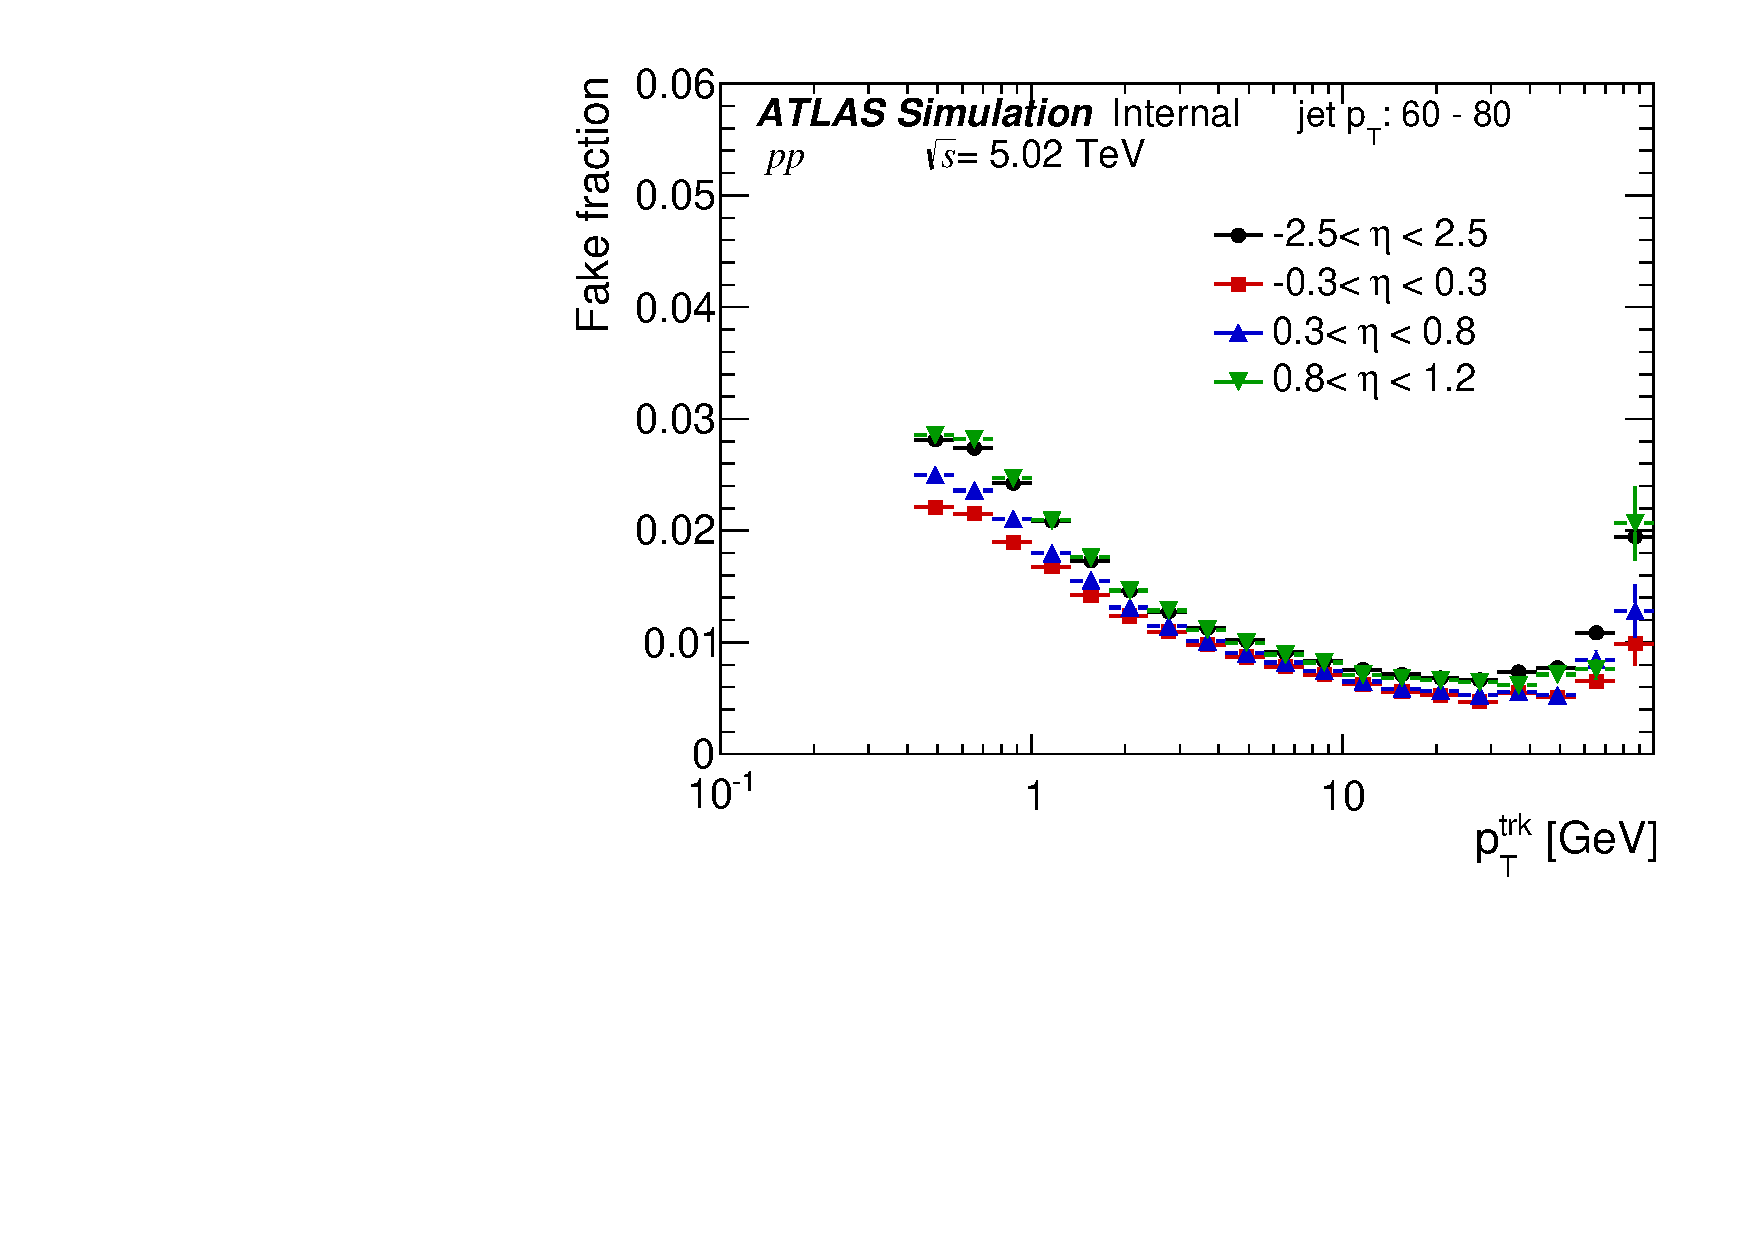
\includegraphics[width=0.45\textwidth]{figures/main/corrections/fake_rates/FakesEta_pp_5p02_r003_Tight_mcprob0p3_JZ2_jetpt_2.pdf} &
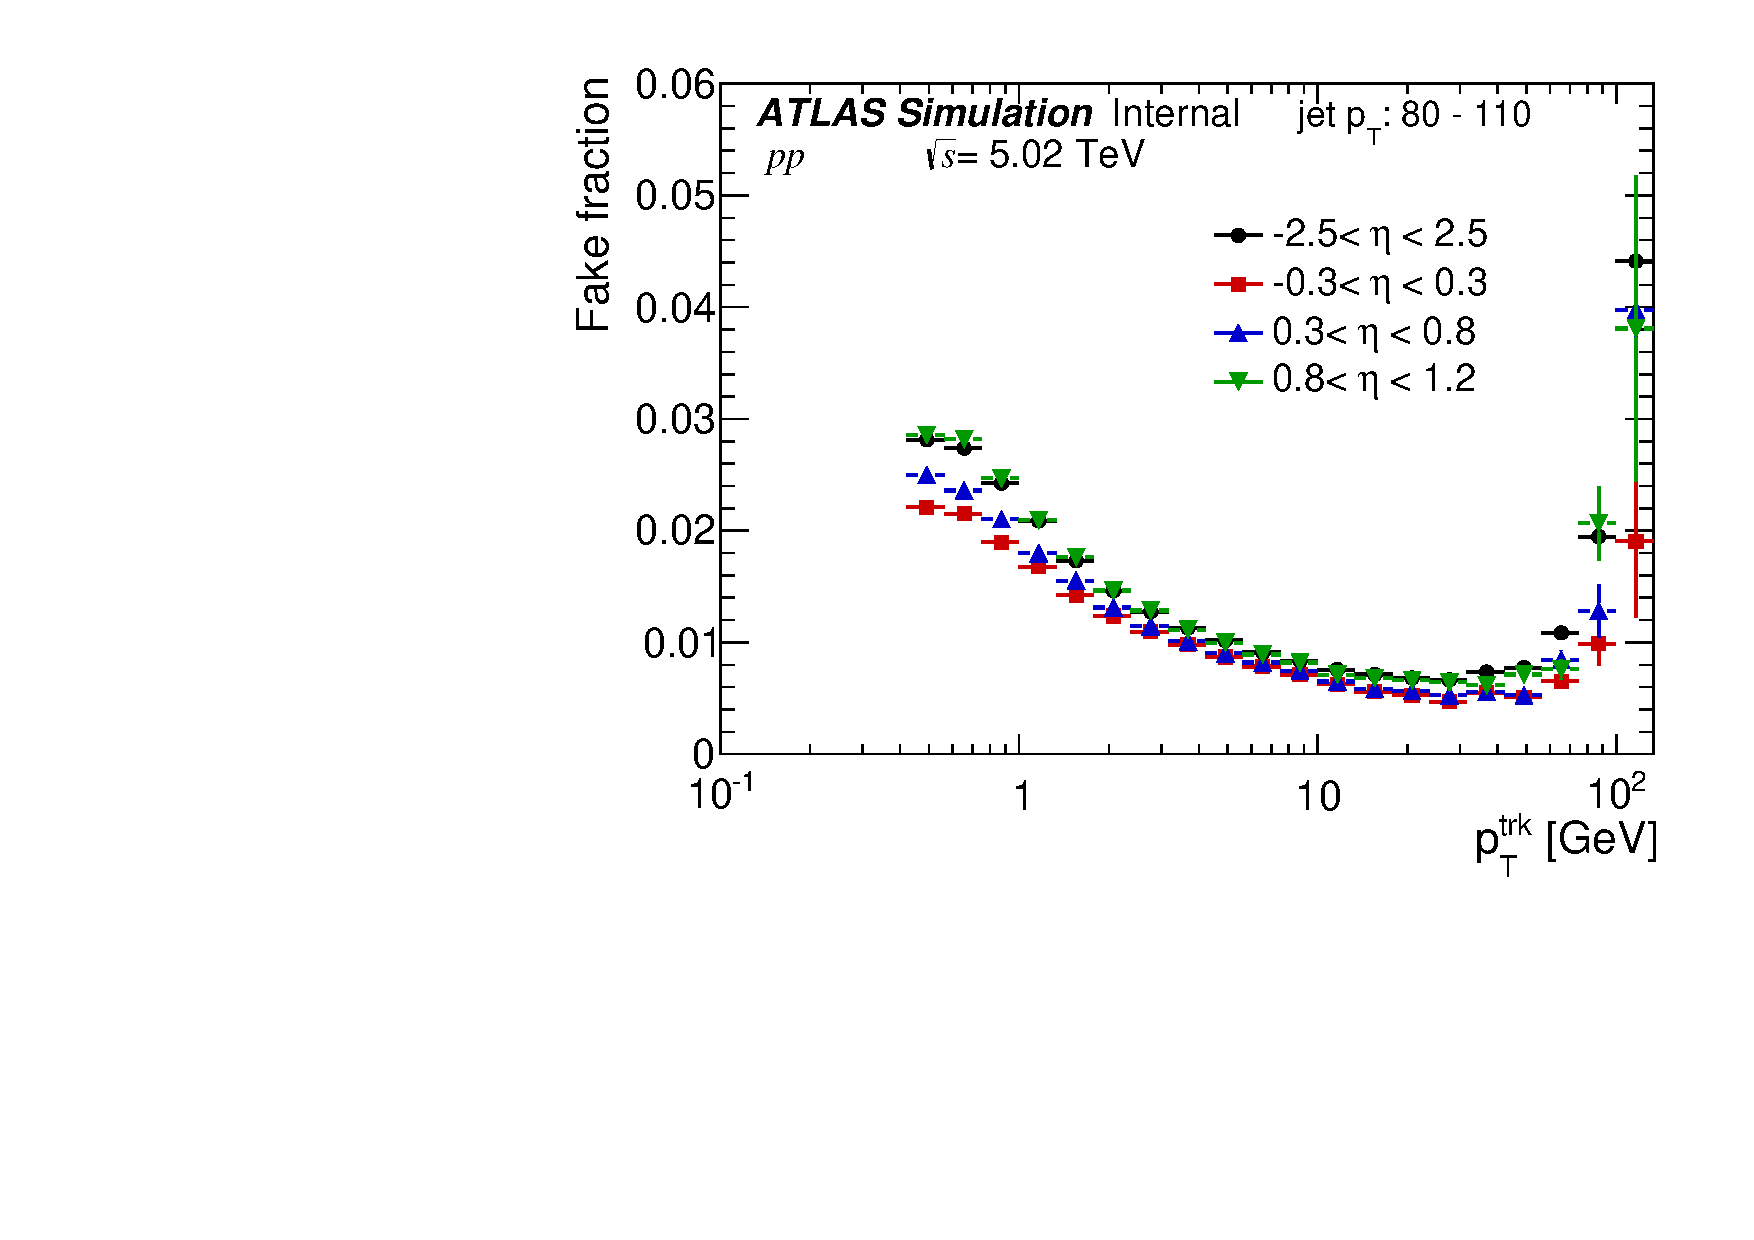
\includegraphics[width=0.45\textwidth]{figures/main/corrections/fake_rates/FakesEta_pp_5p02_r003_Tight_mcprob0p3_JZ2_jetpt_3.pdf} \\
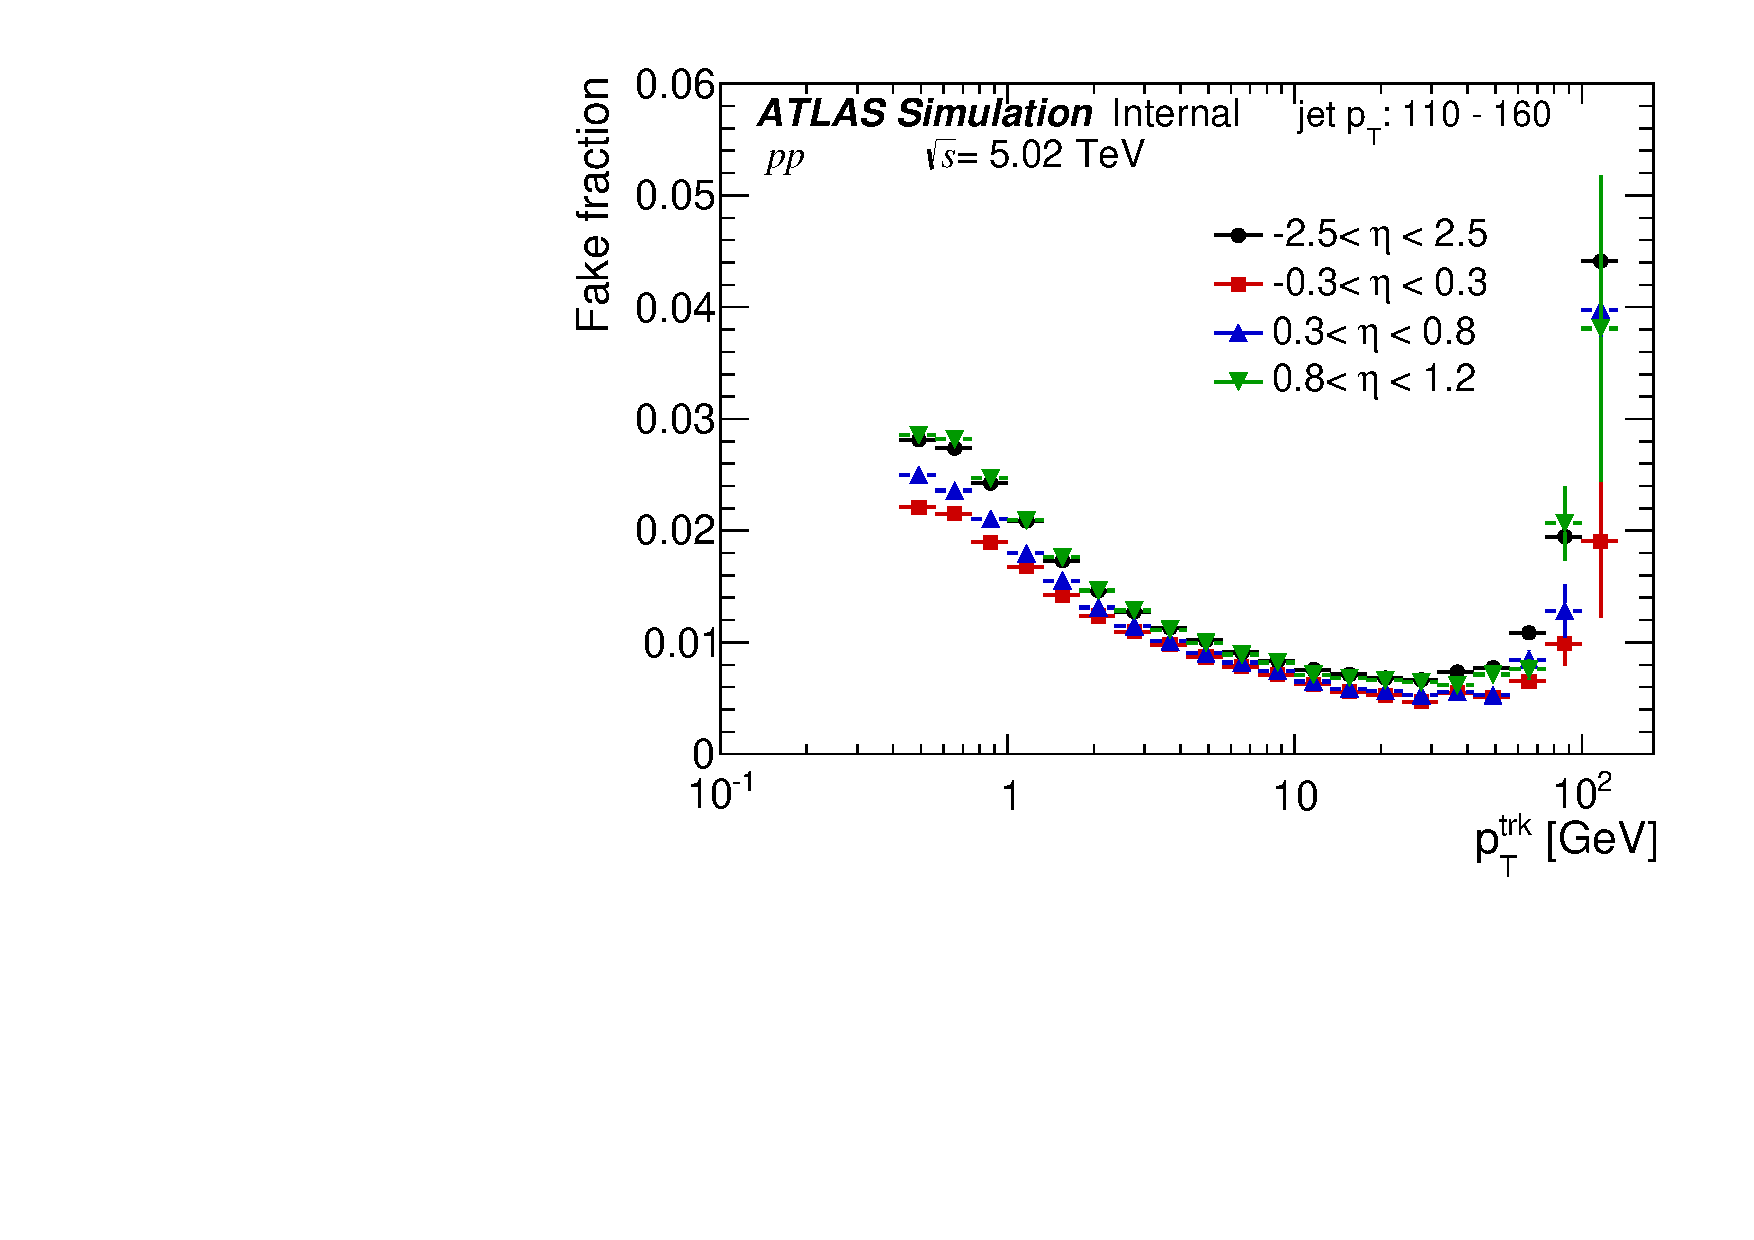
\includegraphics[width=0.45\textwidth]{figures/main/corrections/fake_rates/FakesEta_pp_5p02_r003_Tight_mcprob0p3_JZ2_jetpt_4.pdf} &
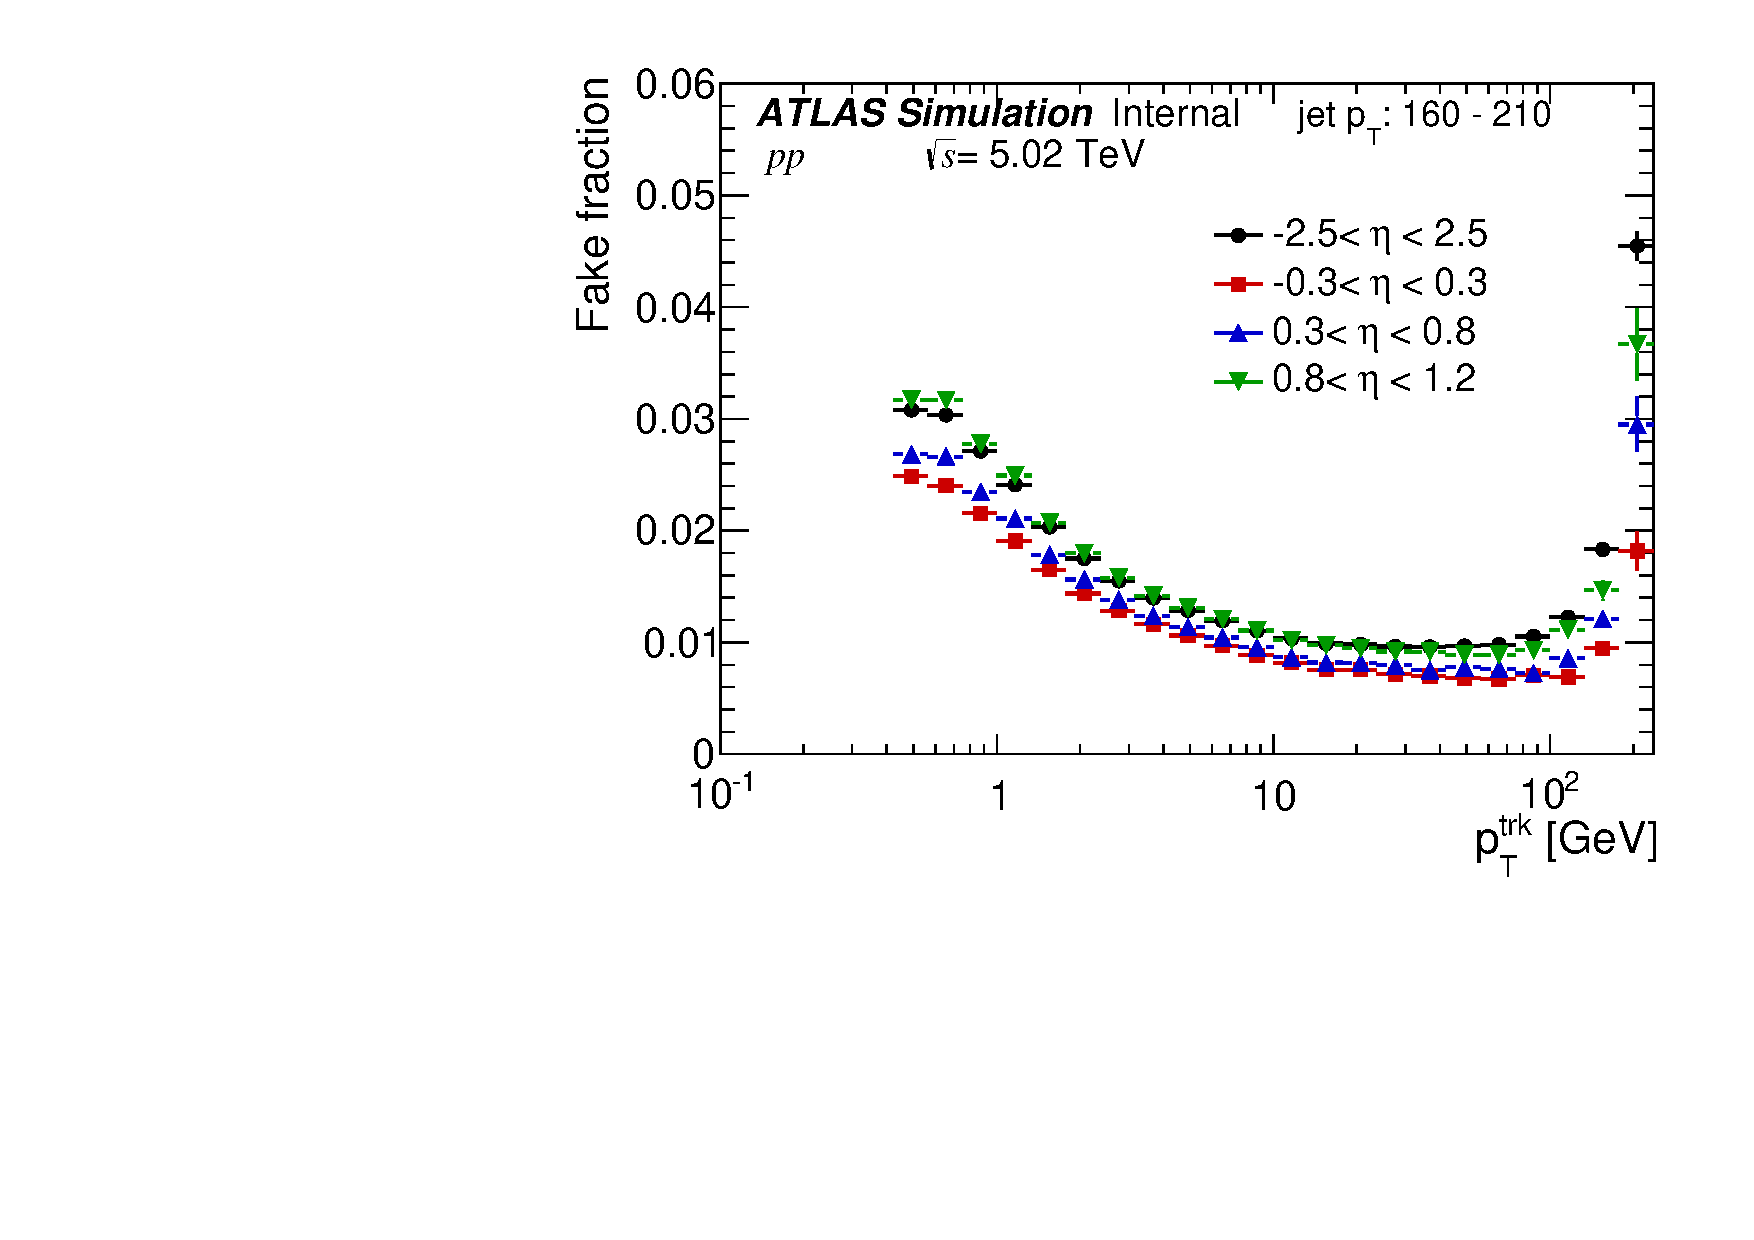
\includegraphics[width=0.45\textwidth]{figures/main/corrections/fake_rates/FakesEta_pp_5p02_r003_Tight_mcprob0p3_JZ3_jetpt_5.pdf} \\
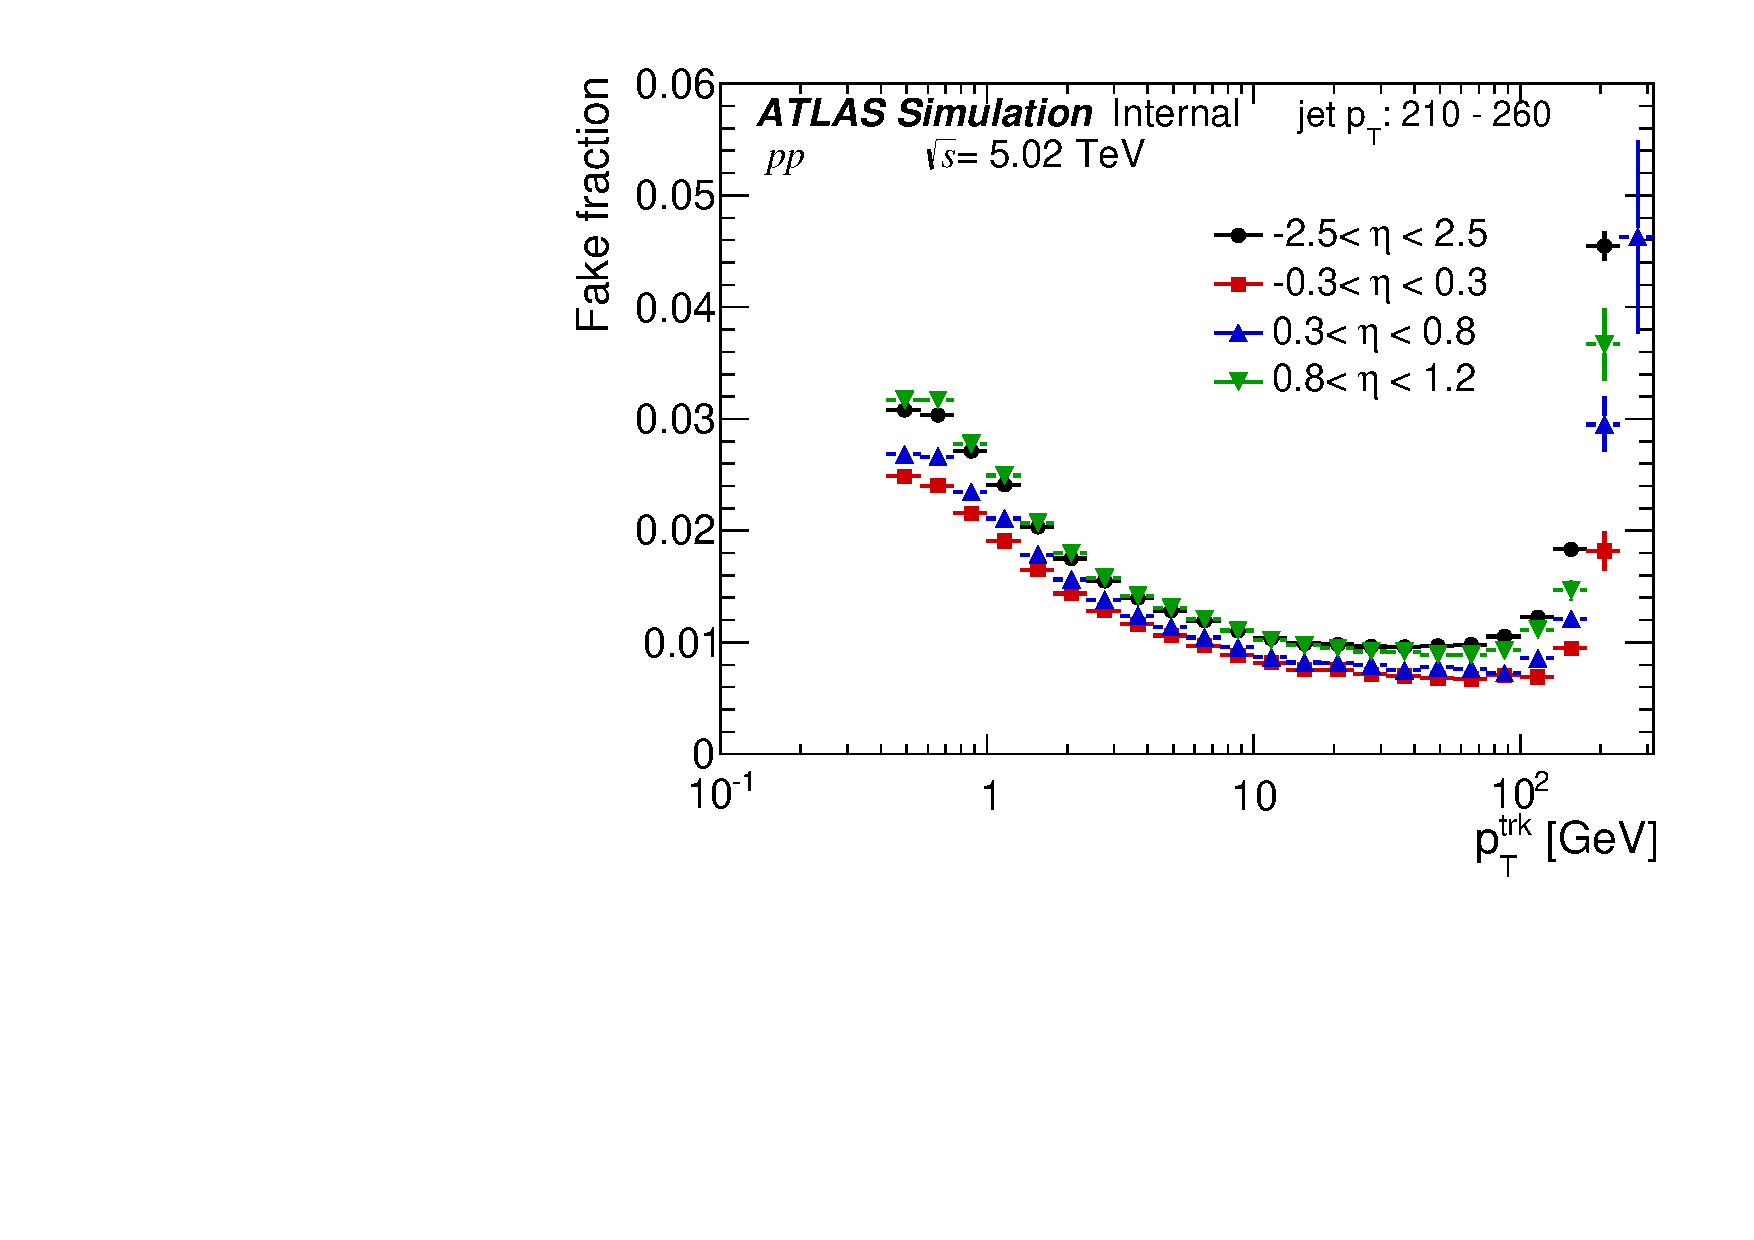
\includegraphics[width=0.45\textwidth]{figures/main/corrections/fake_rates/FakesEta_pp_5p02_r003_Tight_mcprob0p3_JZ3_jetpt_6.pdf} &
\end{tabular}
\caption{Fake rate for five different \ptjet\ selections in 5.02 TeV \pp\ collisions and four pseudorapidity intervals.
The fake rate is evaluated for default value of \mcprob\ cut of 0.3 used in 2015 analysis.
Figure taken from Ref.~\cite{Sickles:2235420}.}
\label{fig:fakeratepp}
\end{figure}  

\begin{figure}
\centering
\begin{tabular}{cc}
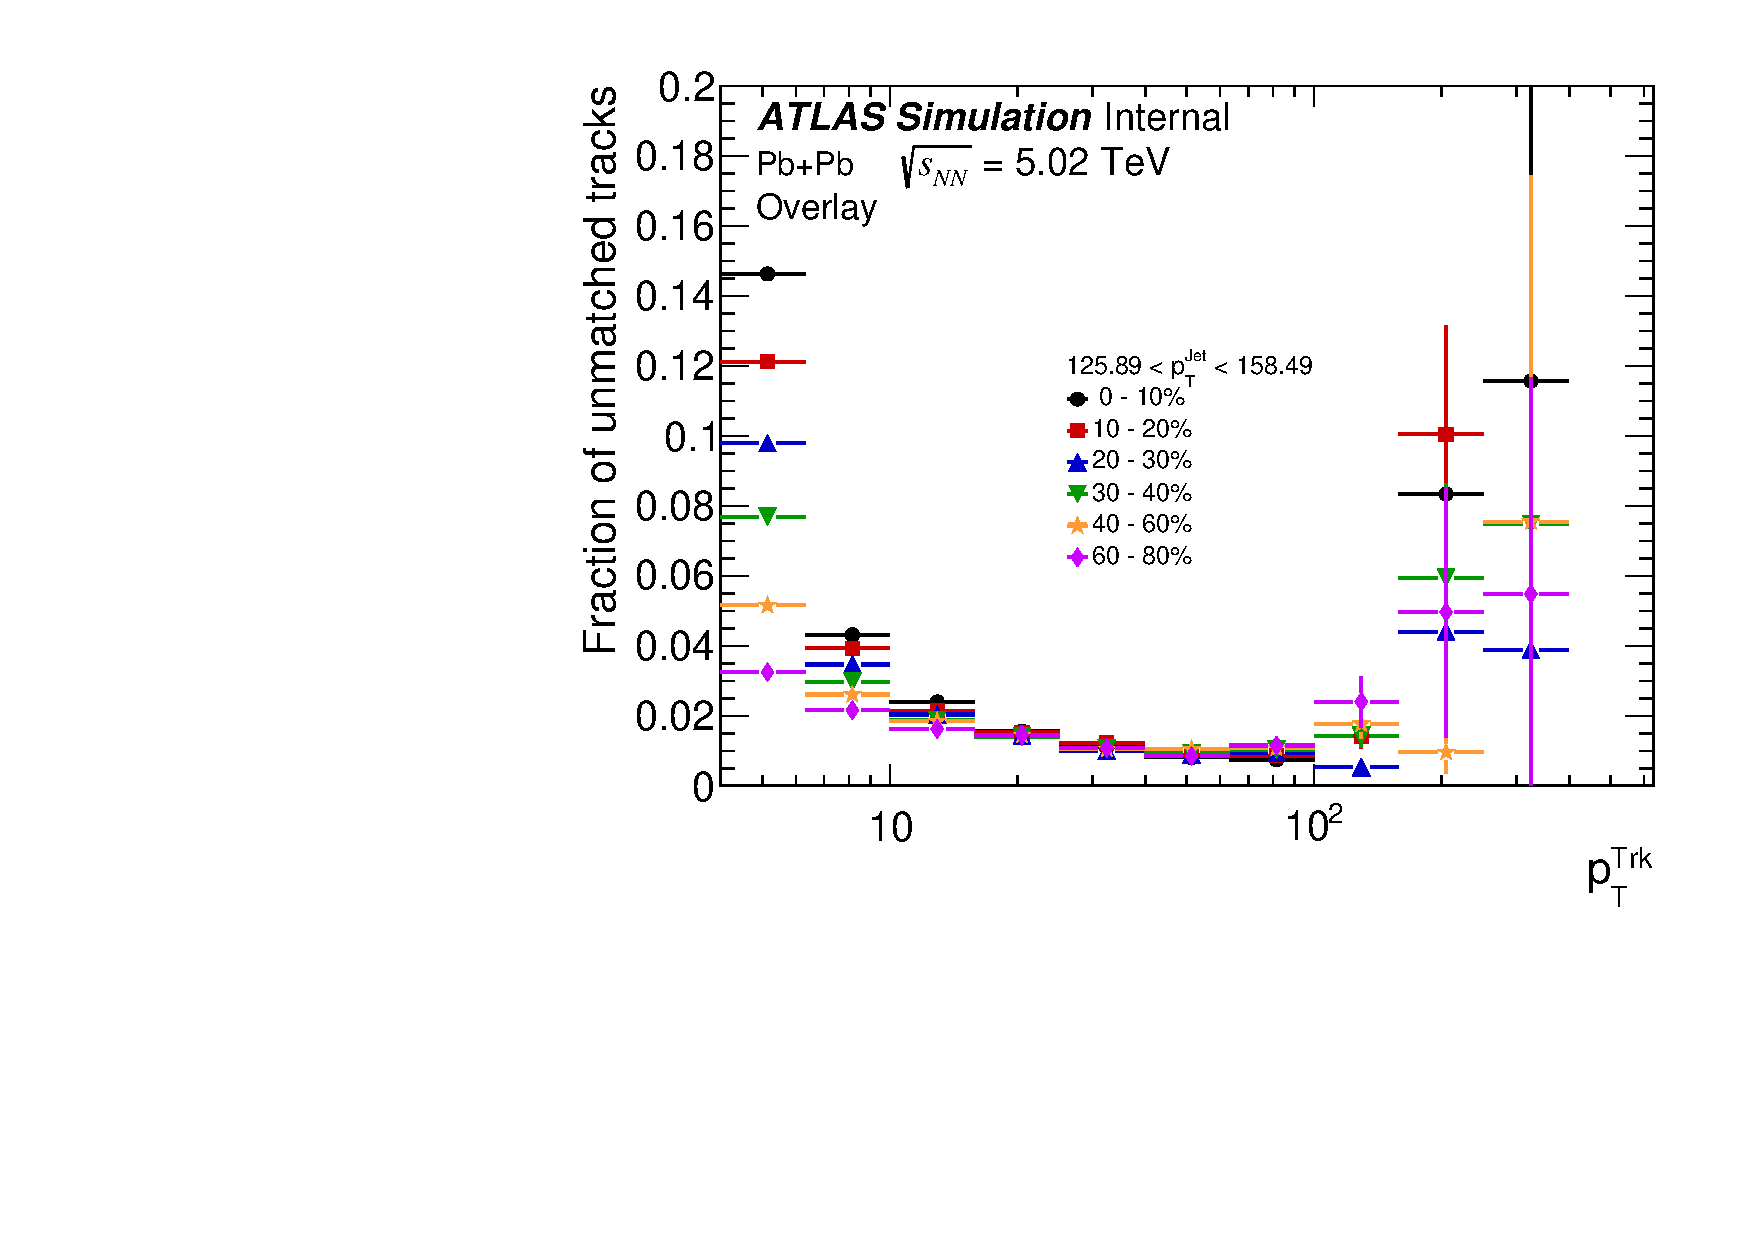
\includegraphics[width=0.45\textwidth]{figures/main/corrections/fake_rate_pt_125GeV.pdf} &
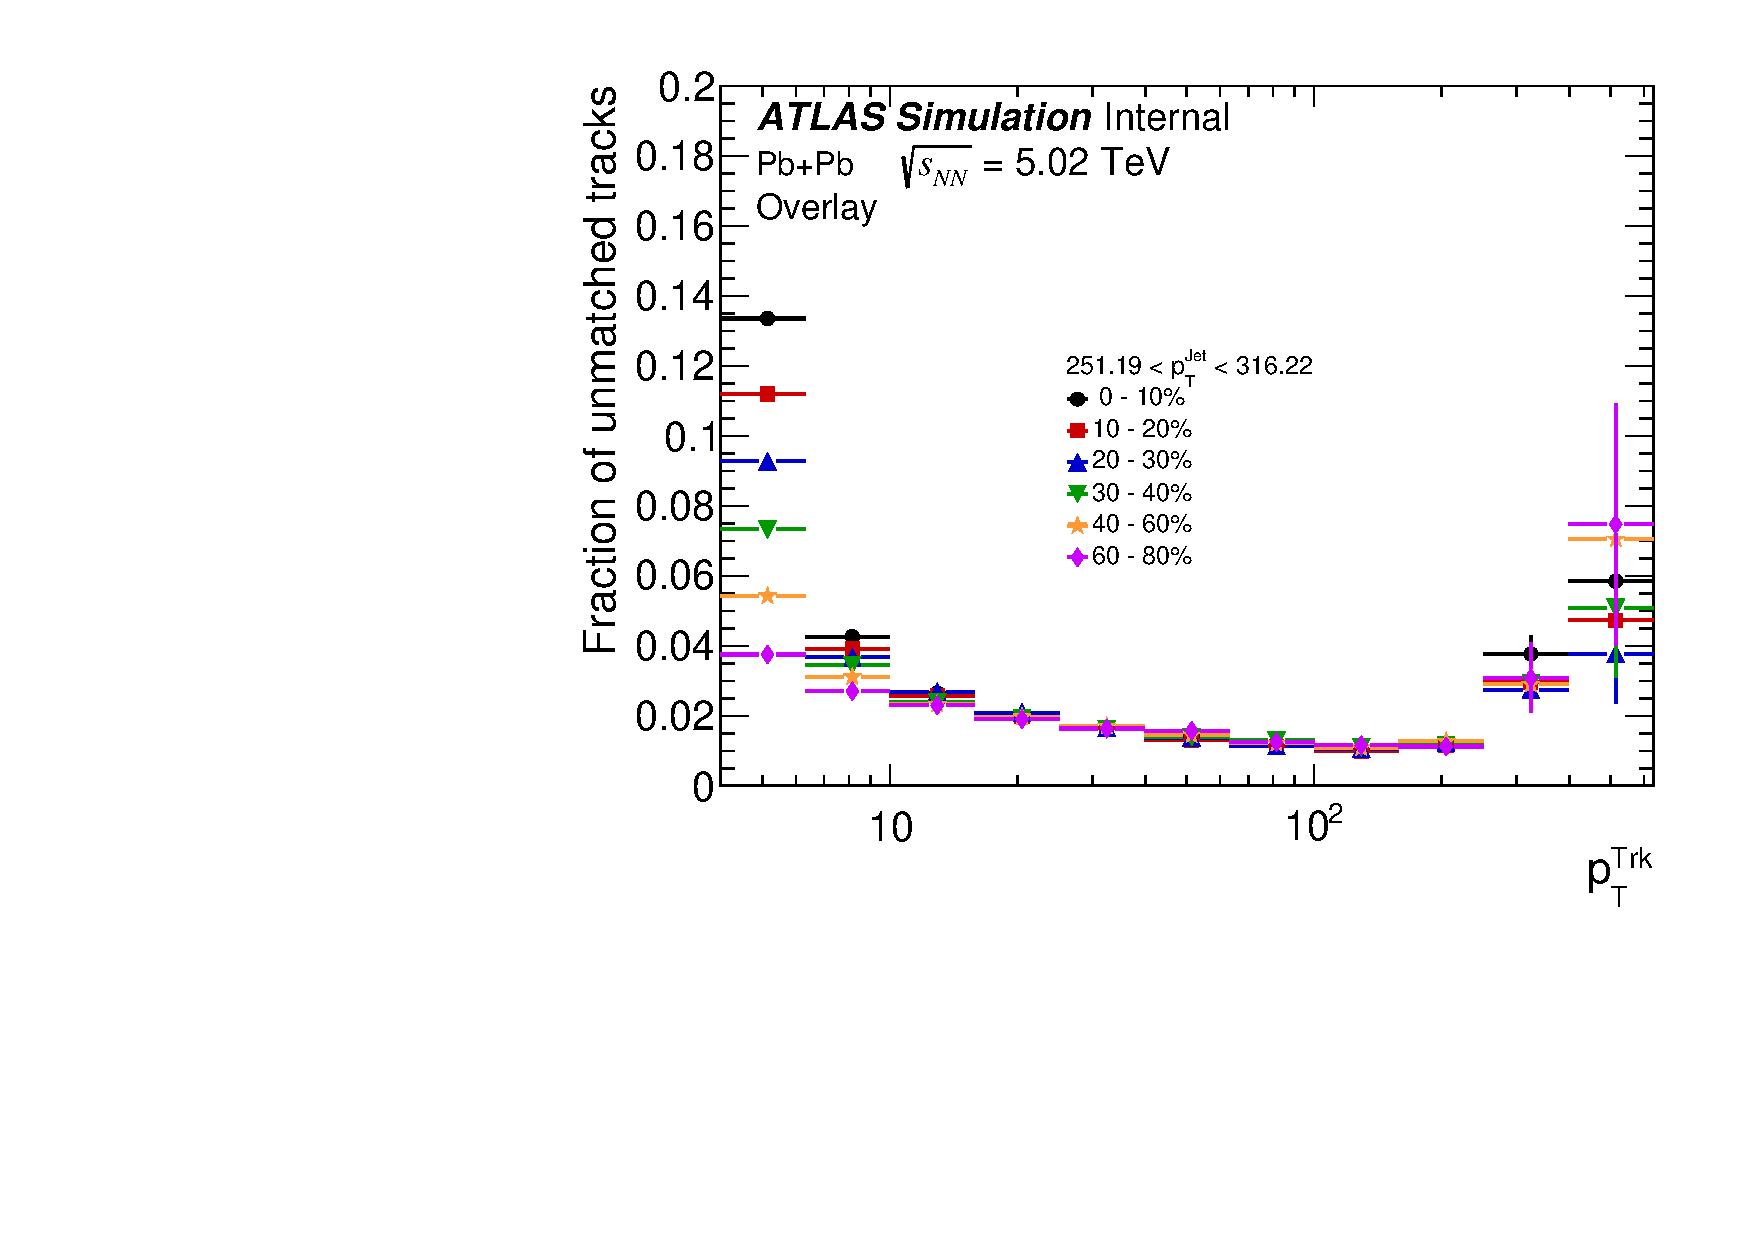
\includegraphics[width=0.45\textwidth]{figures/main/corrections/fake_rate_pt_251GeV.pdf} \\
\end{tabular}
\caption{ Rate of tracks unmatched to truth tracks
in \pbpb\ collisions for different centrality selections as indicated on the plot as a function of \pttrk.
The unmatched tracks include both fake tracks and tracks from the underlying event.
The panels show two \ptjet\ selections: 126-158~GeV (left) and 251-316~GeV (right).
The low \pT\ part is omitted as it is dominated by the contribution from the UE.
Figure taken from Ref.~\cite{Sickles:2235420}.}
\label{fig:fakeratepbpb}
\end{figure}
\begin{figure}
\centering
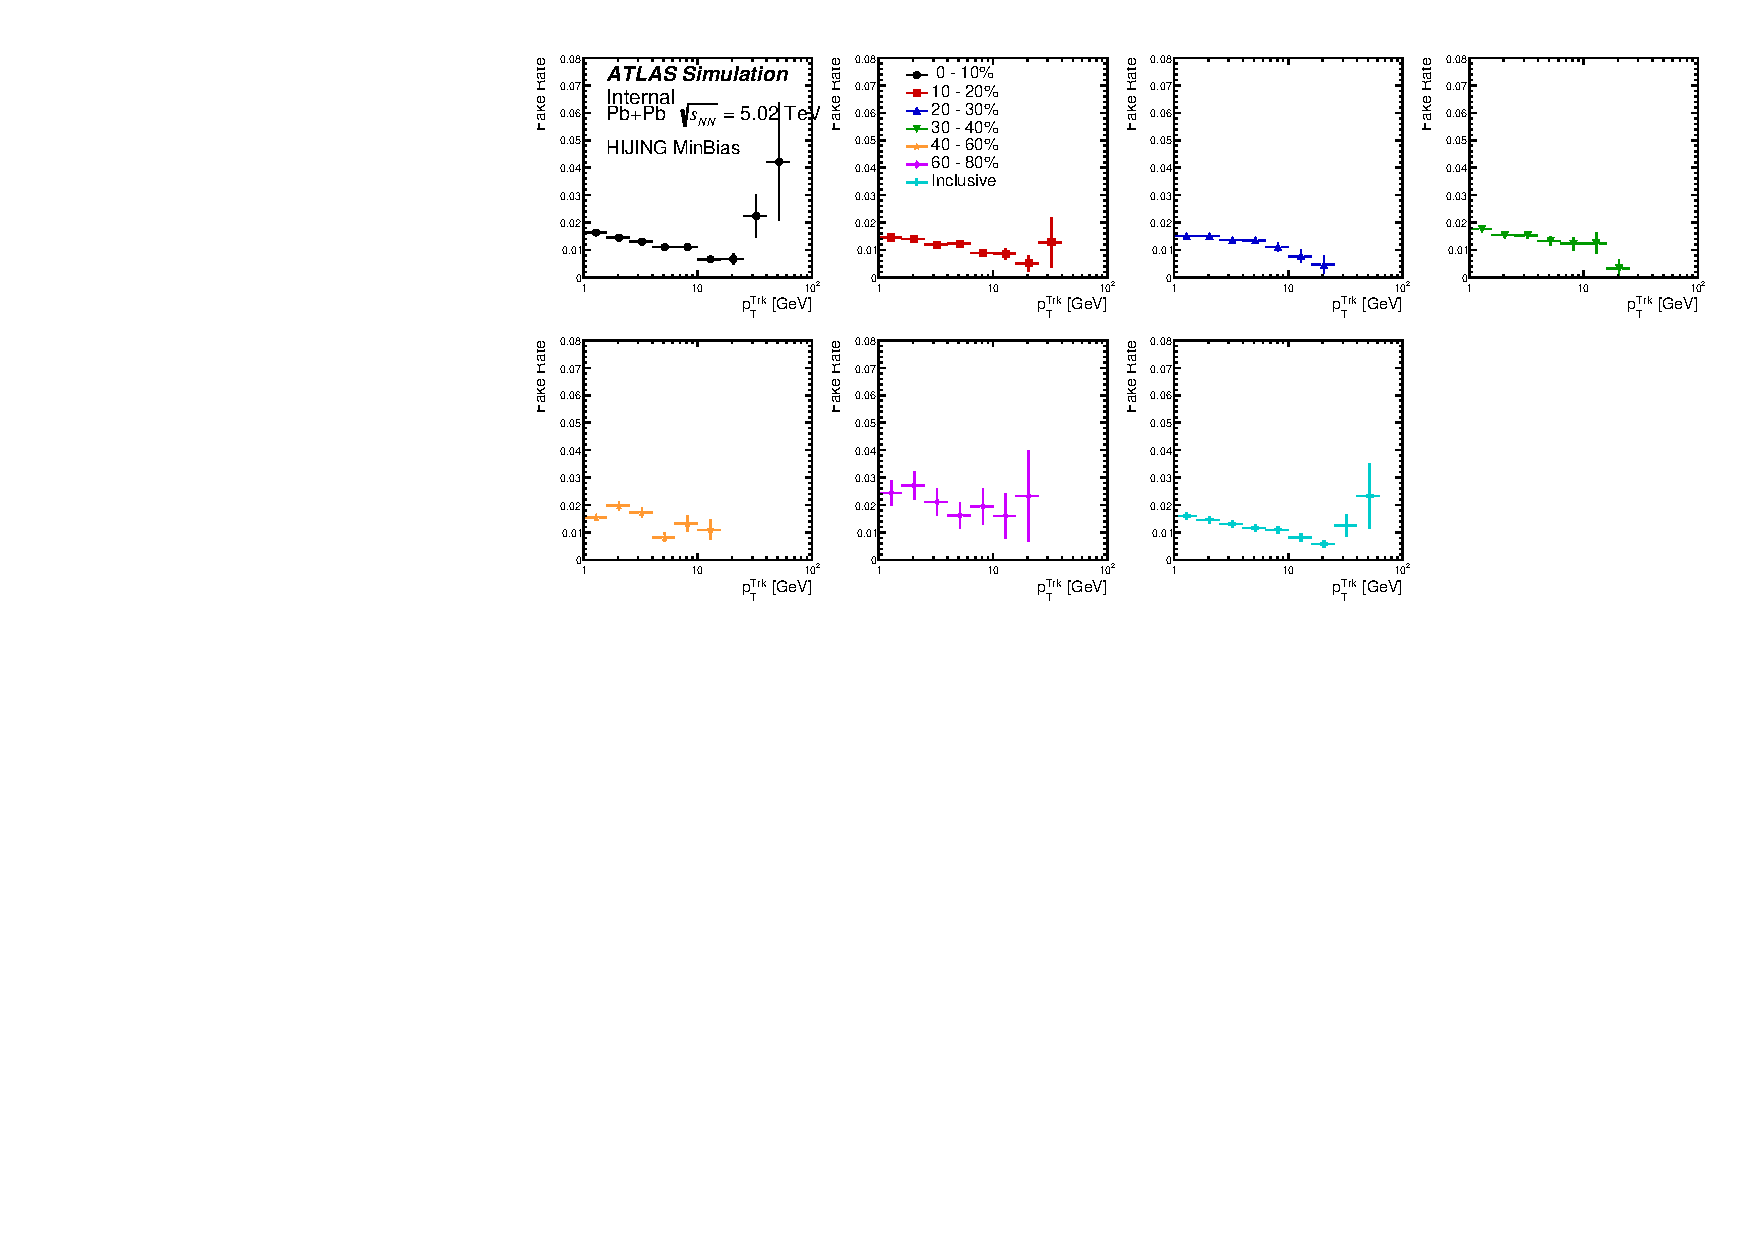
\includegraphics[width=1.\textwidth]{figures/main/performance/fake_rate_hijingMB.pdf}
\caption{ Fake rate for six different centrality intervals in 5.02 TeV \pbpb\ HIJING MC collisions.
The fake rate is evaluated for default value of $\mcprob = 0.3$ in 2015 analysis.}
\label{fig:fakeratehijing}
\end{figure}


To correct for the contribution from fake and secondary particles, charged particle distributions are estimated using reconstructed tracks that do not have a truth match as defined by criteria described in previous paragraphs.
These distributions are then subtracted from the measured distributions both in the data and MC.
This procedure is applied for tracks above 10 GeV in \PbPb\ collisions and for tracks above 1 GeV in \pp\ collisions.
The correction also removes any residual UE above 10~GeV in case of \PbPb.
The choice of the 10 GeV cut is based on the centrality dependence of the rate of truth-unmatched tracks in MC overlay samples shown in Figure~\ref{fig:fakeratepbpb}.
The correction for UE, fake and secondary tracks below 10 GeV in \PbPb\ collisions is discussed in the next section.


%%%%%%%%%%%%%%%%%%%%%%%%%%%%%%
\subsection{Underlying event subtraction of tracks}
\label{sec:cuts_UE}
The underlying event subtraction performed on the calorimetric jet energy is described in Sec.~\ref{sec:reconstruction}.
Charged particles from the nucleon-nucleon scatterings that are not associated with the hard scattering in question constitute a background to the \Dptr\ distributions that needs to be subtracted from the measured distributions.
This background strongly depends on the collisions centrality and on the charged particle \pt.
In the measurement of the inclusive jet fragmentation functions it was found that the UE contribution is negligible for charged particles with $\pt>10$~GeV~\cite{PhysRevC.98.024908}.
This can be seen in the centrality dependence of the combined rate of fake and underlying event charged particles shown in Figure~\ref{fig:fakeratepbpb} where no significant centrality dependence is observed for track above 10 GeV.

In \pp\ collisions, the UE is not subtracted.
The pileup contribution is negligible and subtracting the intrinsic UE from the hard scattering processes would also necessitate a similar subtraction in the particle level fragmentation functions in \pbpb\ that would be generator dependent and make comparisons between \pp\ and \pbpb\ non-trivial.

In \pbpb\ collisions, the UE from the soft processes is estimated using two independent methods.
The ``Map method" is nominally used for the analysis while the ``Cone method" is used to provide a systematic uncertainty.
The former uses charged particle distributions of $\mathrm{d}N_{\mathrm{ch}}/\mathrm{d}\phi\mathrm{d}\eta(\mathrm{cent},\pt, \mathrm{d}\Psi_{\mathrm{ch}})$ in MC overlay events, while the latter evaluates the underlying event on an event-by-event basis using a grid of cones.

%%%%%%%%%%%%%%%
\subsubsection{Map Method}
\label{sec:map_method}
In the "Map Method", $\eta-\phi$ maps of the average number of UE charged particles in a given annulus around a jet ($\nchUE^{\mathrm{Map}}$) are determined in MC overlay events using tracks without a truth match.
The maps are filled as a function of the distance from the jet, \ptjet, \etajet, \phijet, angle of the jet to the reaction plane\footnote{The reaction plane angle $\Psi$ is determined on an event-by-event basis by a standard method using the $\phi$ variation of transverse energy in the forward calorimeter} $ \mathrm{d}\Psi_{\mathrm{ch}}$, \pt\ and centrality.

Examples of the these distributions for three different annuli (0--0.05, 0.25 -- 0.30, 0.60--0.70), in the $\mathrm{d}\Psi$ interval of  0.80 -- 1.00, for six collision centrality classes and for 1--1.6 GeV particles in 126 -- 158 GeV jets are shown in Figure~\ref{fig:ue_map}.
The number of UE particles associated with a jet decreases with size of the annulus, decreasing centrality, increasing track \pT\ and increasing distance to the reaction plane.

\begin{figure}
\begin{subfigure}{.5\textwidth}
\centering 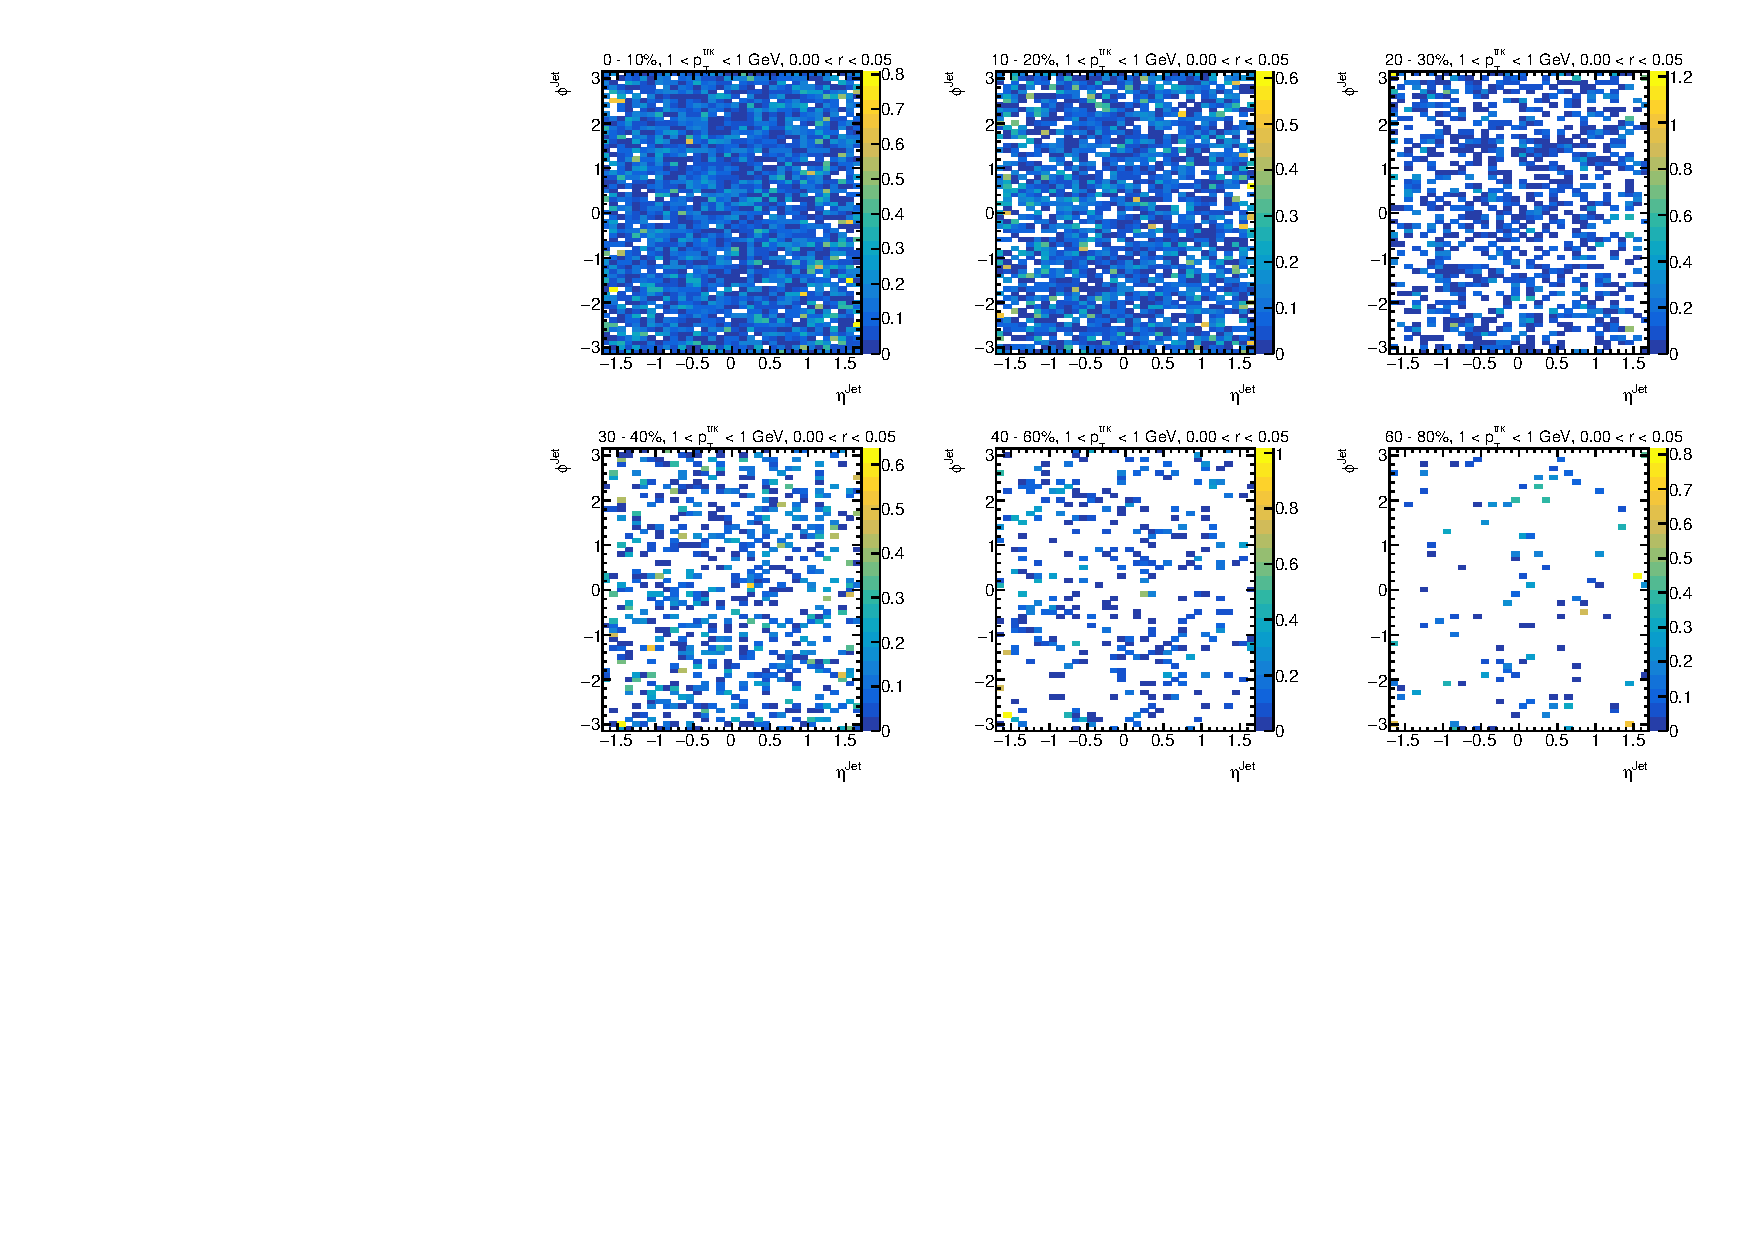
\includegraphics[width=1\textwidth]{figures/main/UE/eta_phi_map_trk2_dR0}
\caption{}
\end{subfigure}
\begin{subfigure}{.5\textwidth}
\centering 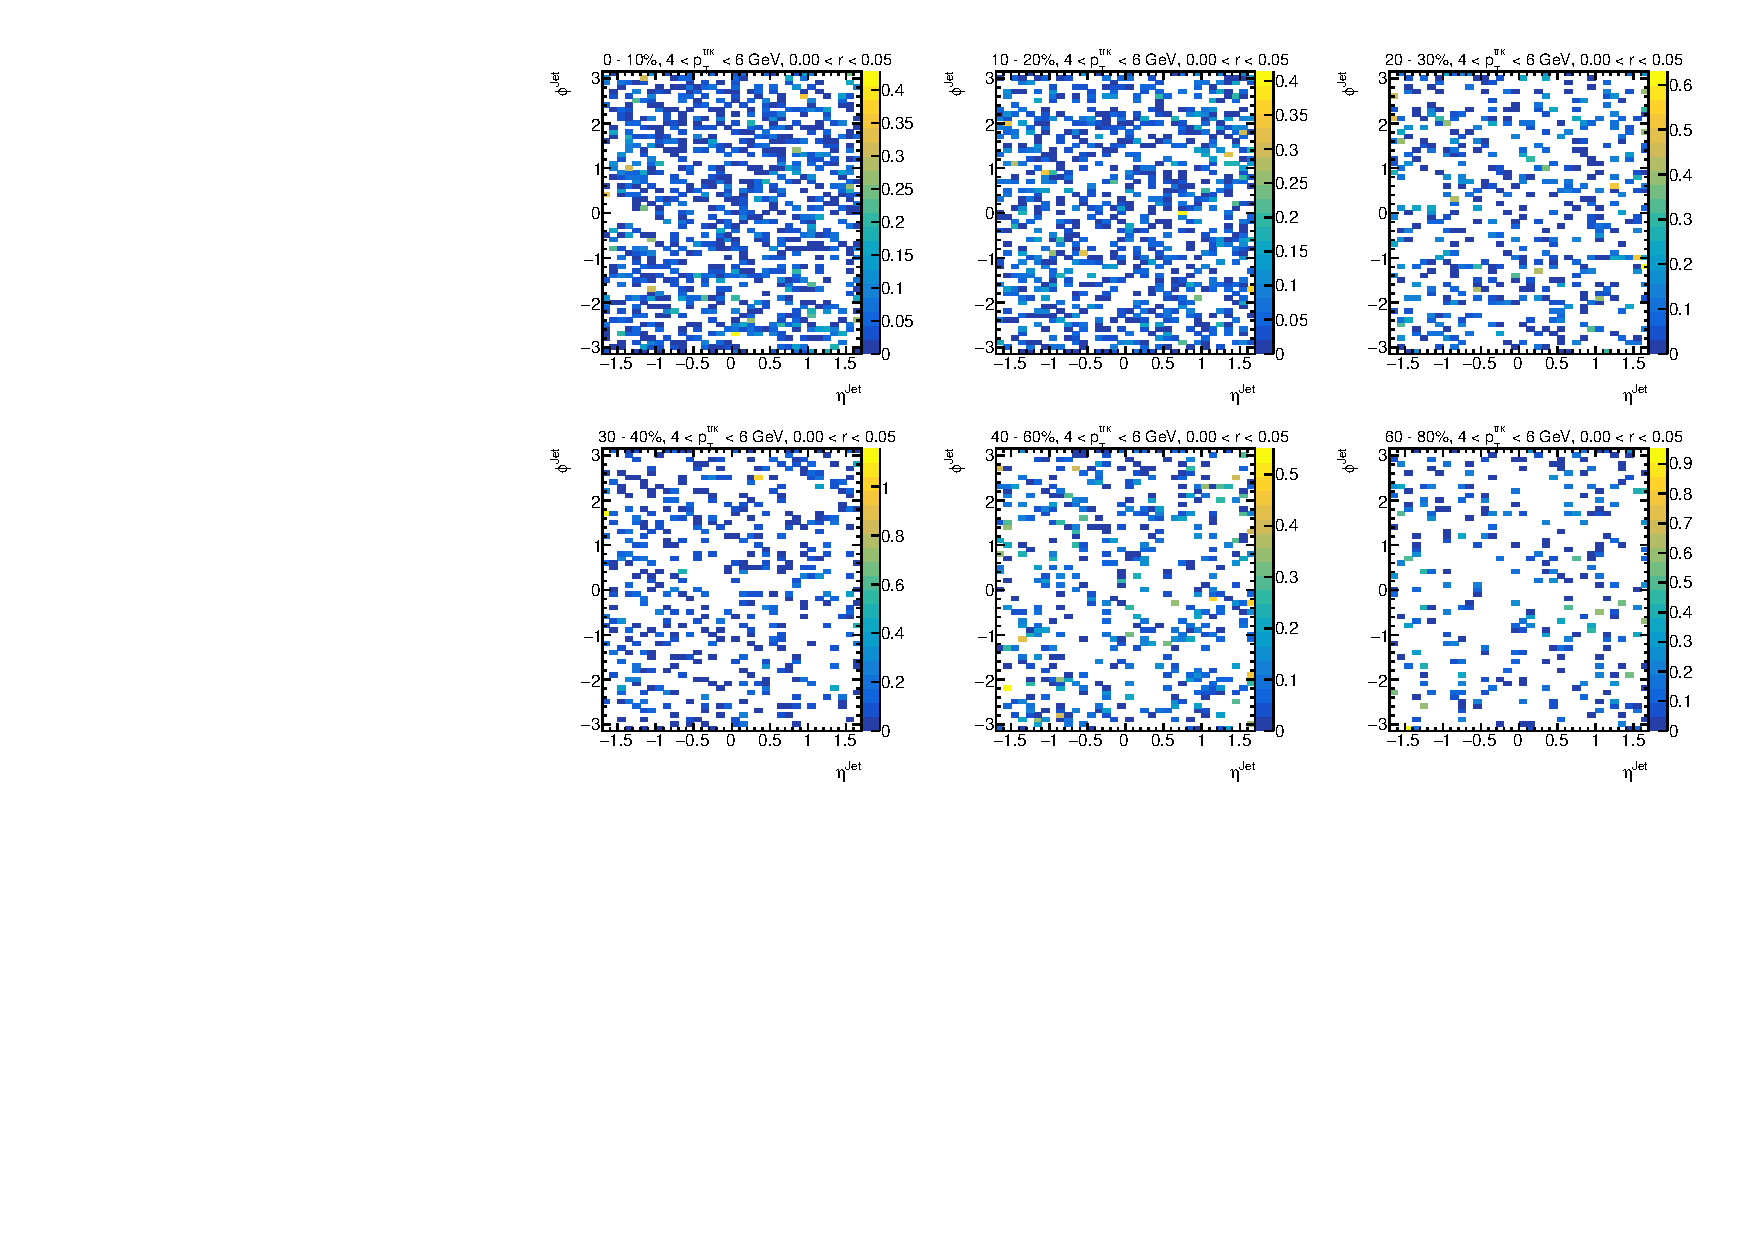
\includegraphics[width=1\textwidth]{figures/main/UE/eta_phi_map_trk6_dR0}
\caption{}
\end{subfigure} \\
\begin{subfigure}{.5\textwidth}
\centering 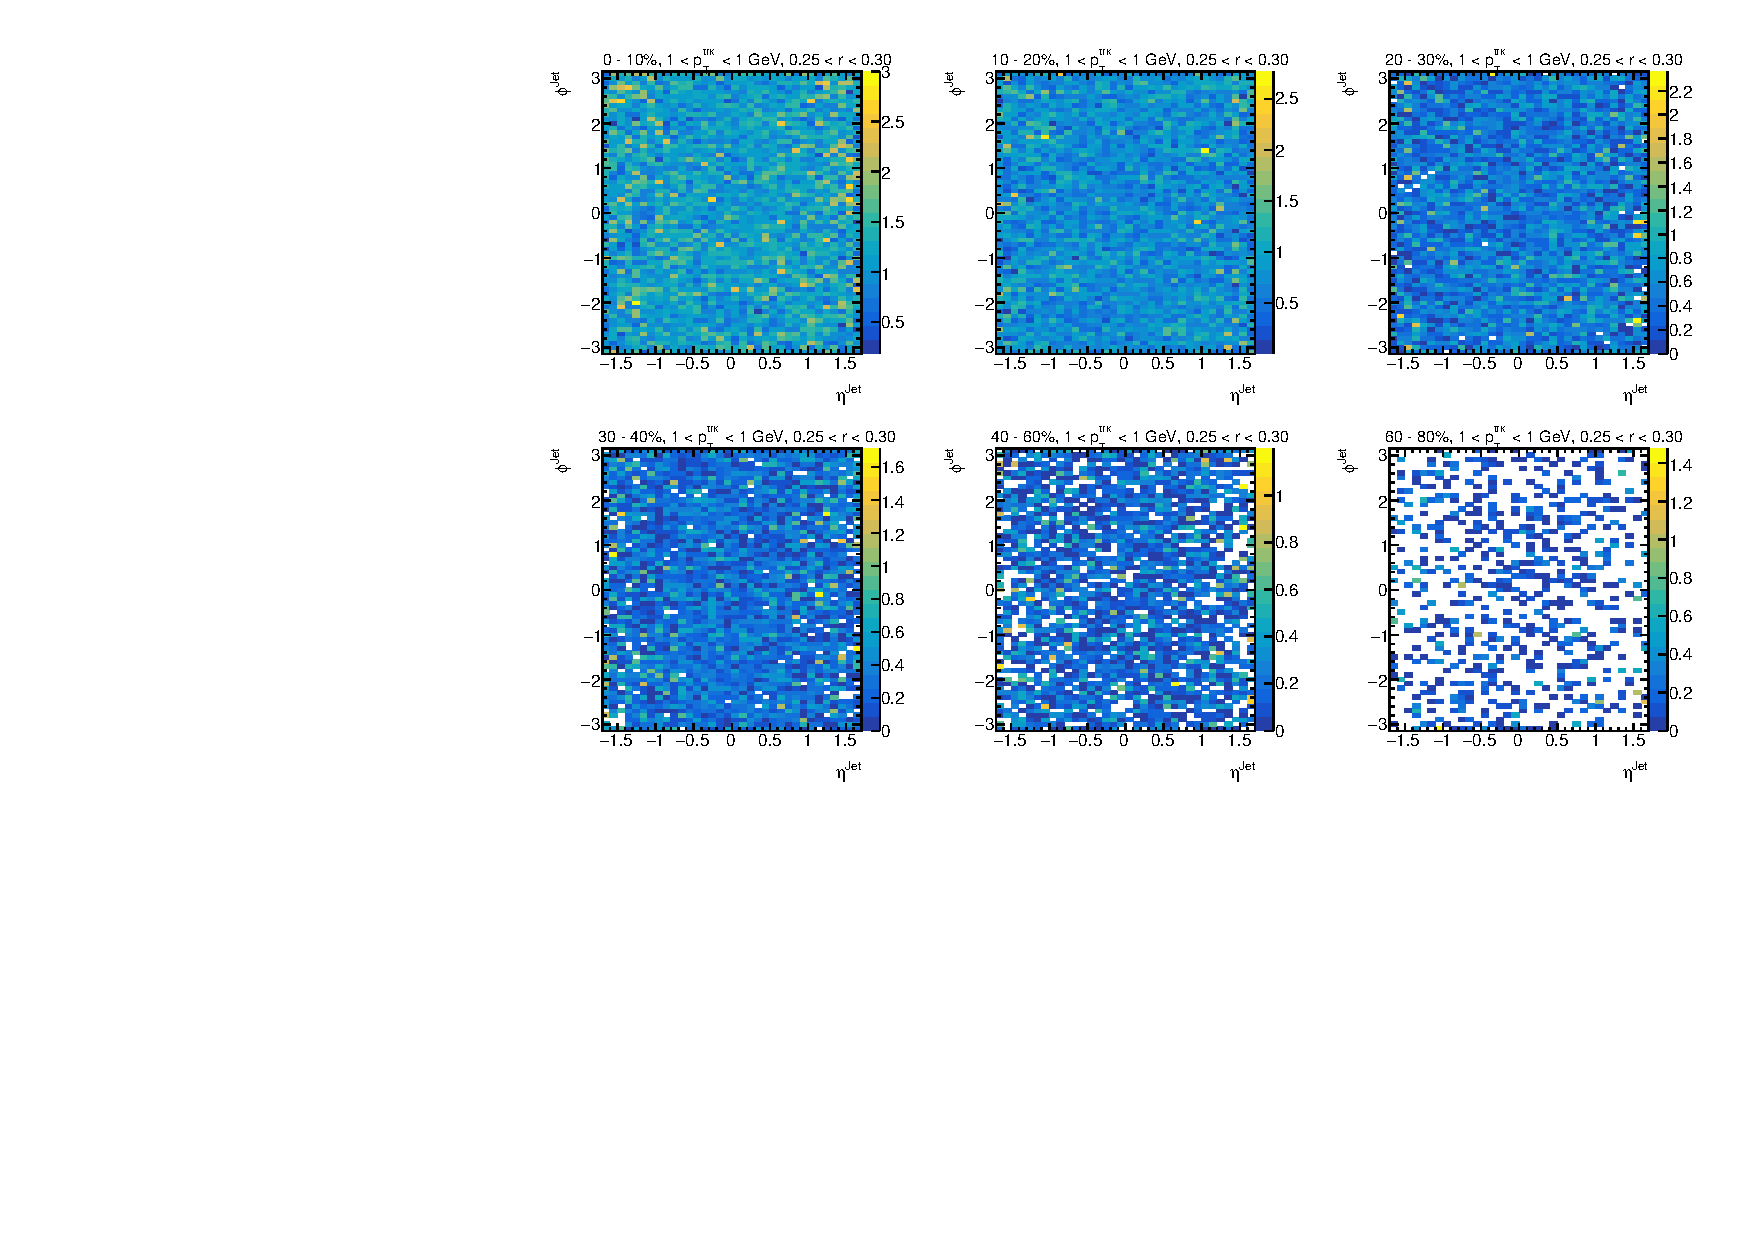
\includegraphics[width=1\textwidth]{figures/main/UE/eta_phi_map_trk2_dR5}
\caption{}
\end{subfigure}
\begin{subfigure}{.5\textwidth}
\centering 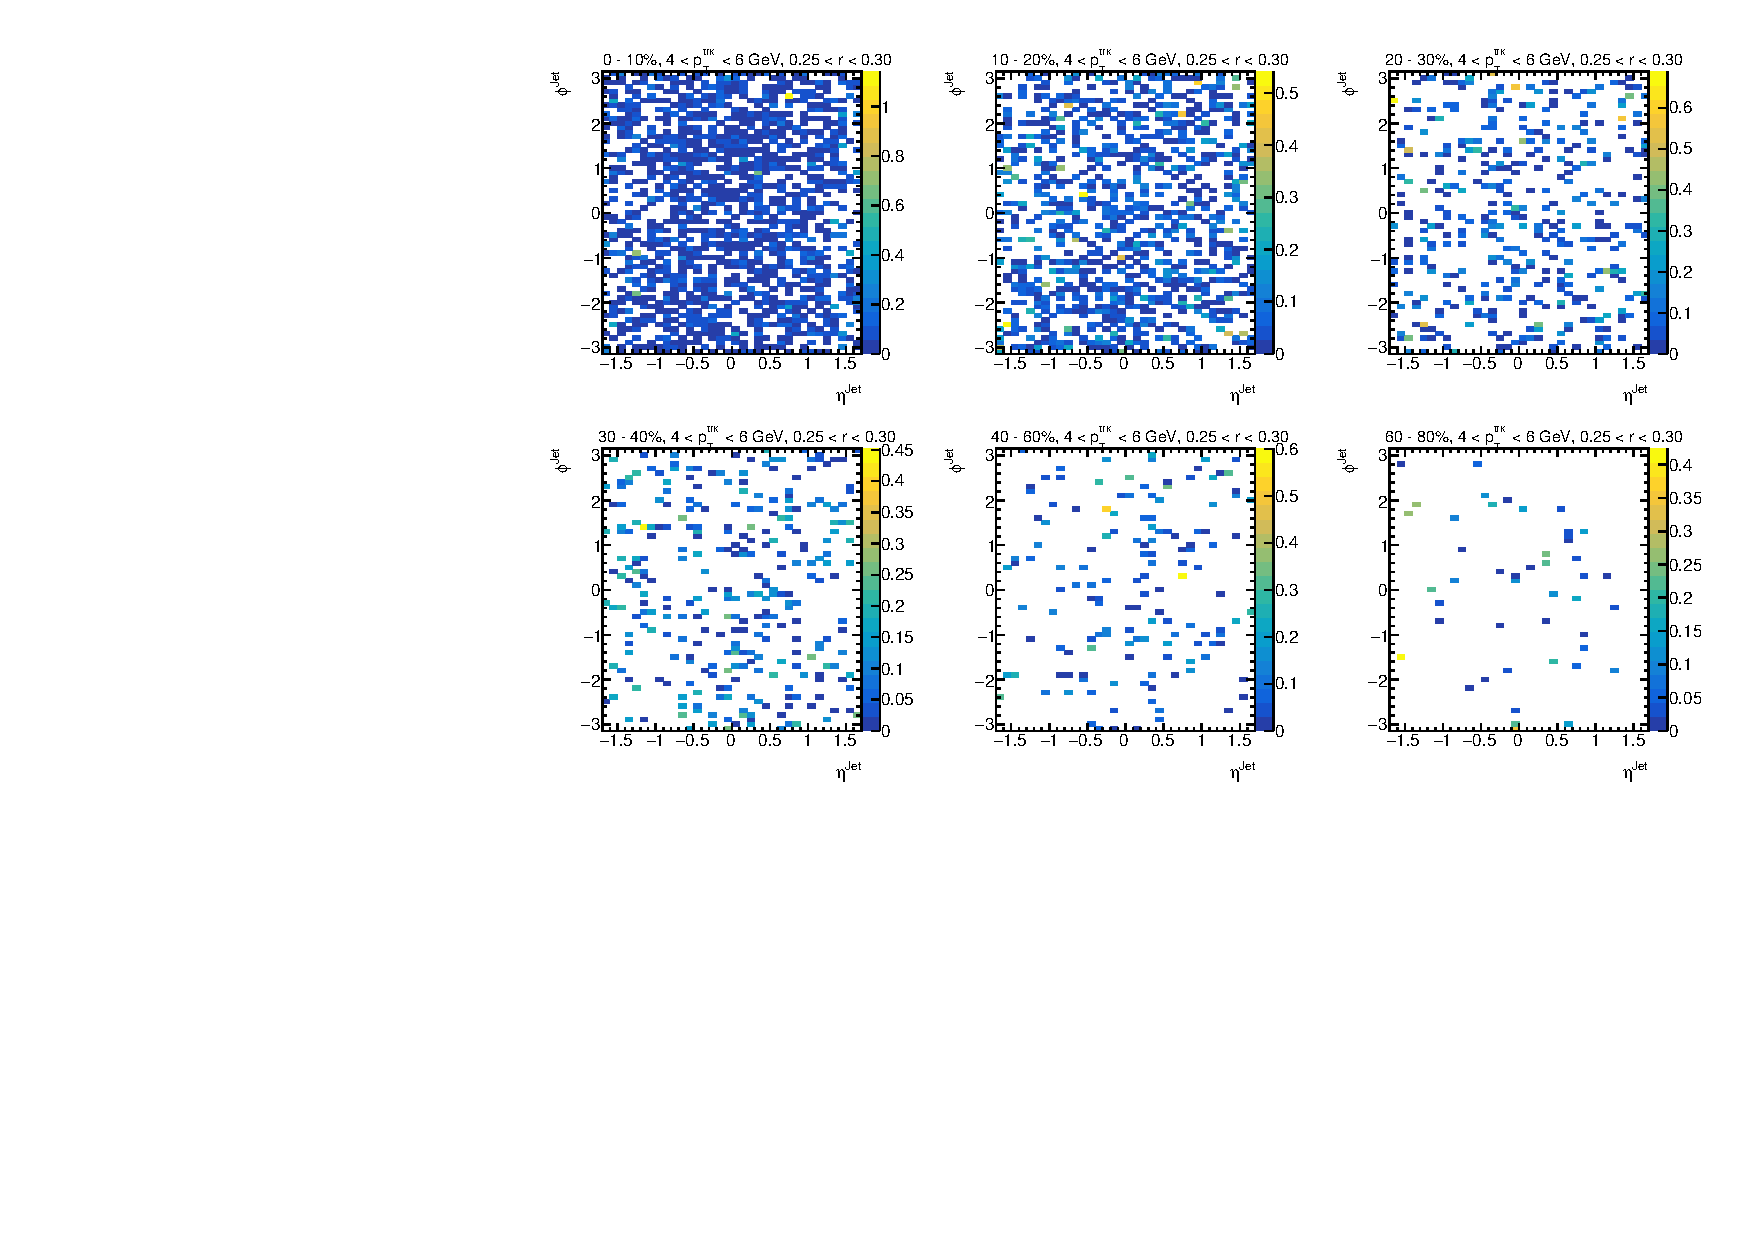
\includegraphics[width=1\textwidth]{figures/main/UE/eta_phi_map_trk6_dR5}
\caption{}
\end{subfigure} \\
\begin{subfigure}{.5\textwidth}
\centering 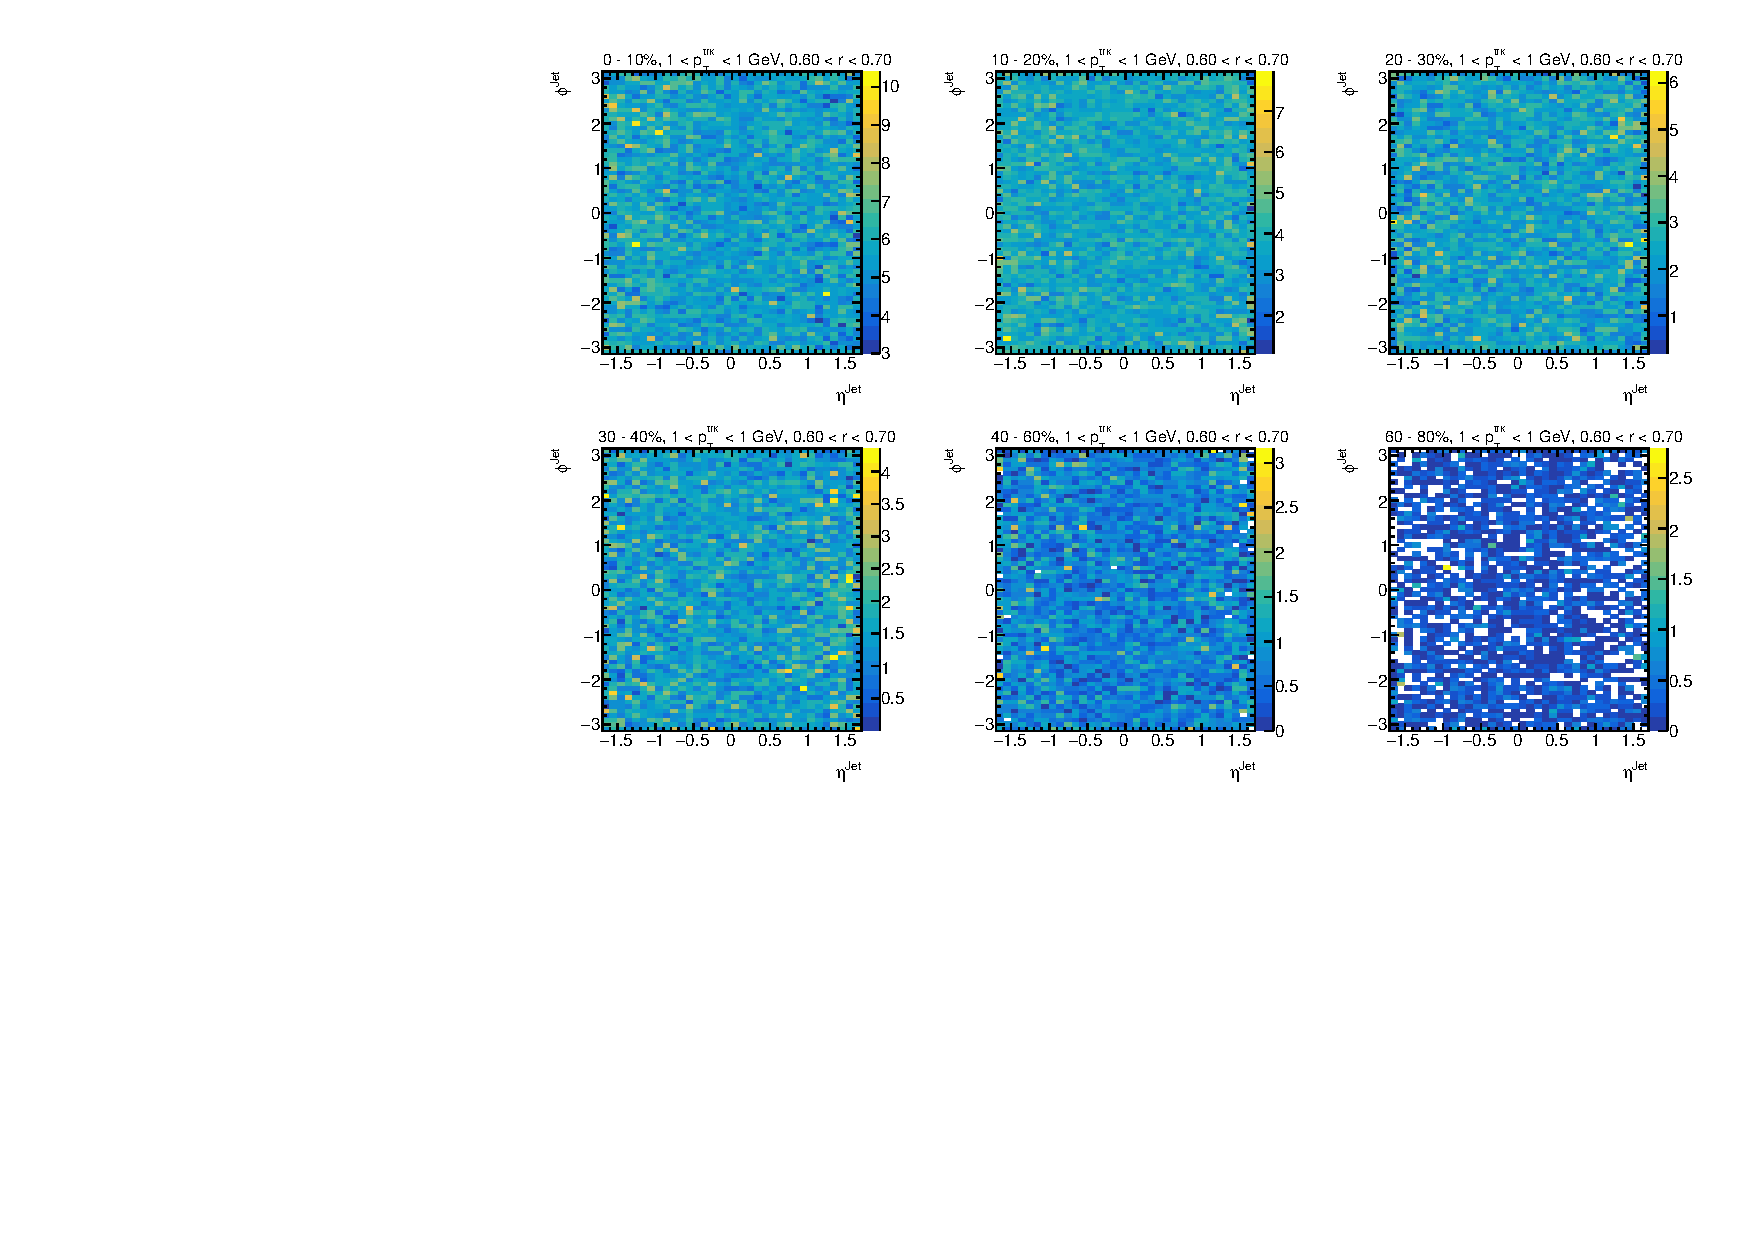
\includegraphics[width=1\textwidth]{figures/main/UE/eta_phi_map_trk2_dR9}
\caption{}
\end{subfigure}
\begin{subfigure}{.5\textwidth}
\centering 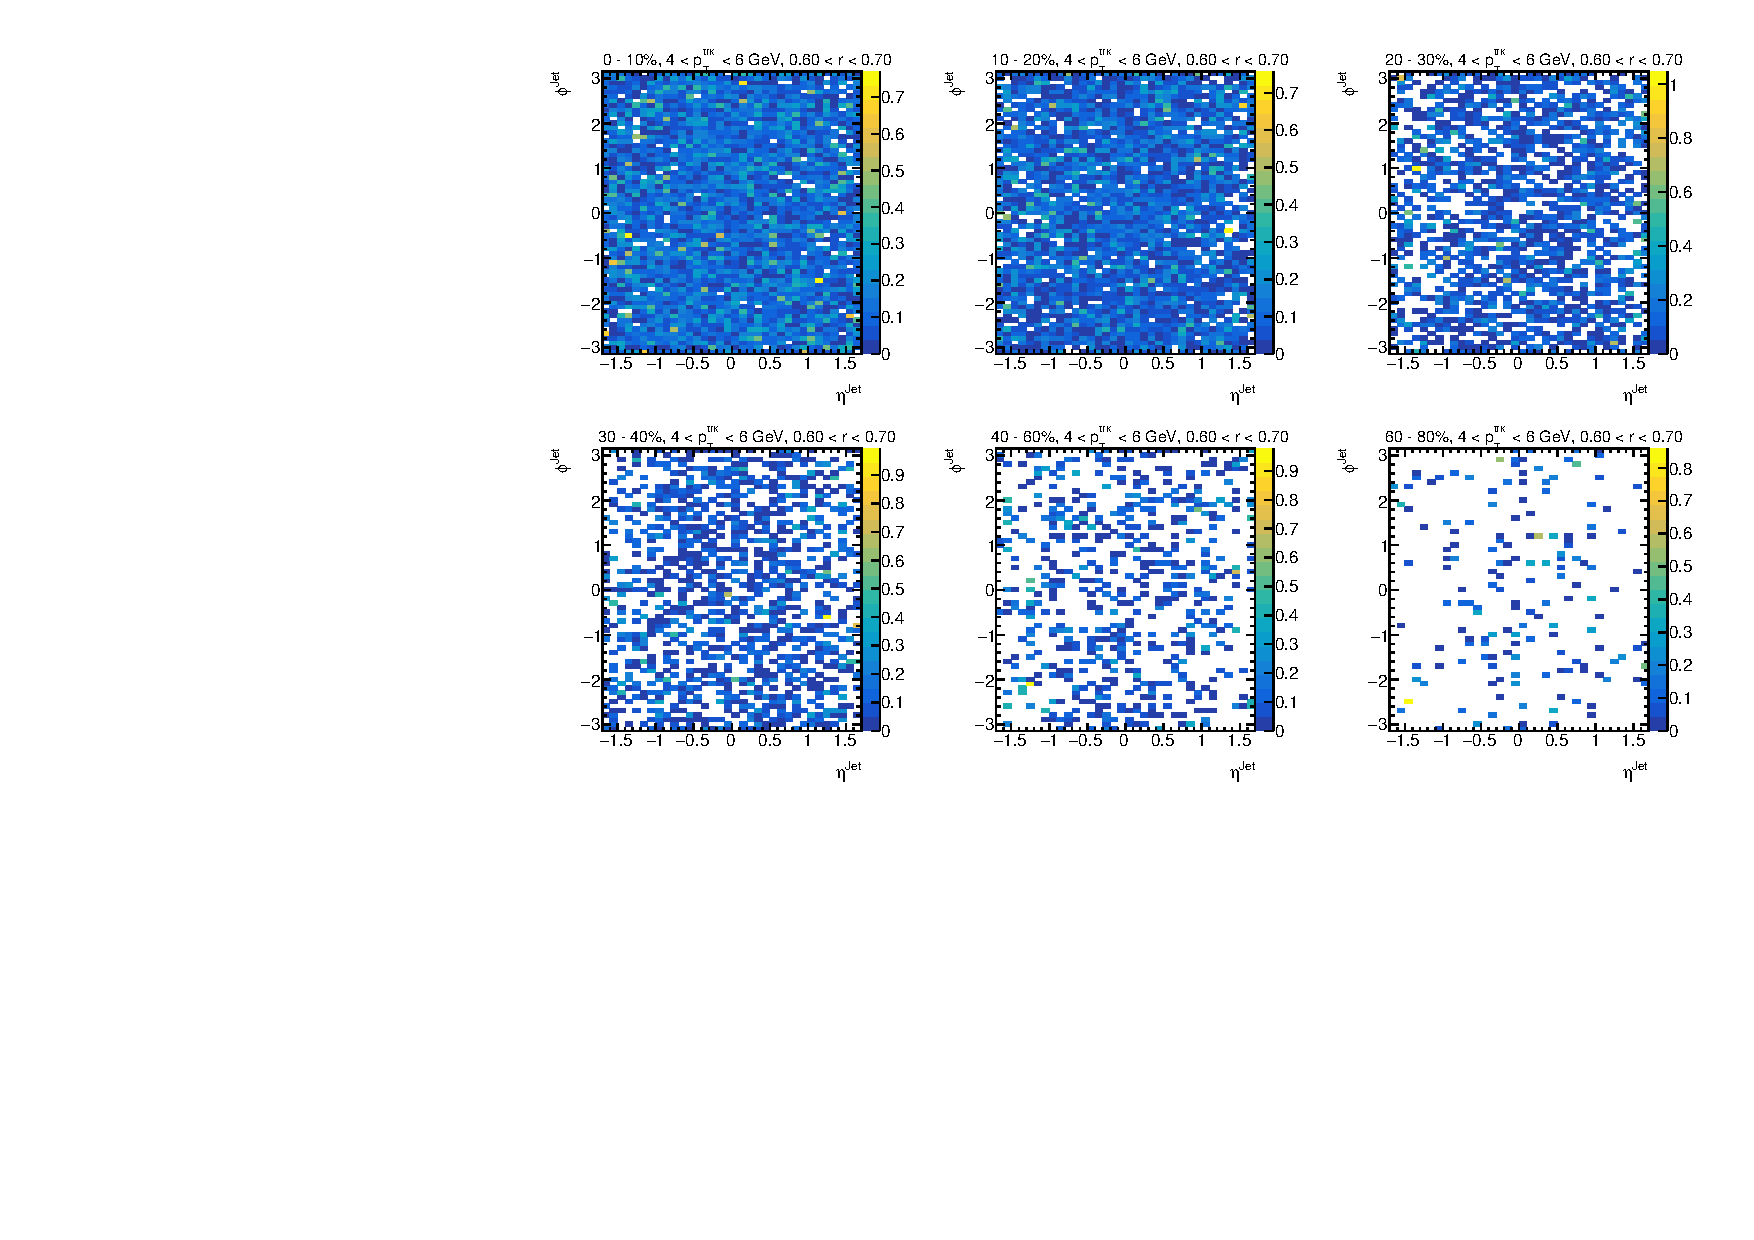
\includegraphics[width=1\textwidth]{figures/main/UE/eta_phi_map_trk6_dR9}
\caption{}
\end{subfigure}
\caption{Per jet $\nchUE^{\mathrm{Map}}$ distributions of charged particles evaluated for 1--1.6 GeV (left) and 4--6 GeV tracks in the jet core (top), near the jet edge (middle), and far from the jet (bottom) for  $\mathrm{d}\Psi$ in the interval 0.8--1.00, for six centralities, and 126--158 GeV jets.}
\label{fig:ue_map}
\end{figure}


The underlying event is then estimated by convoluting the $\nchUE^{\mathrm{Map}}$ distributions with the $\eta_{\mathrm{jet}}$, $\phi_{\mathrm{jet}}$, and $\mathrm{d}\Psi_{\mathrm{jet}}$ distributions of jets.
The UE estimated by this method in MC consists of tracks without a truth match, and hence is the ``true'' underlying event by definition.
This $\mathrm{UE}^{\mathrm{MC}}$ can then be used to correct any correlations between the underlying event as determined by the cone method and the JER (discussed in later sections).
The UE normalized to unit area, as a function of $\Delta R$ with respect to the jet axis is shown in Figure~\ref{fig:UEdR} for the lowest track \pt\ interval where the UE contribution is the largest.
The two distributions are the UE with and without secondary particles.
The UE strongly decreases for more peripheral collisions and for increasing track \pt.
Little radial dependence is seen when the secondaries are not included.
A small effect is expected because there is an enhancement in the number of jets at mid rapidity, along with a decrease in the UE yield as a function of $\eta$.
Since the secondaries are generated by primary PYTHIA particles, the enhancement is expected towards the jet core, where there is a higher multiplicity of primary particles.

%The map method is then applied to data to measure the UE charged particle contribution to the measured \Dptr\ distributions.
%Since this method uses real MB \pbpb\ collisions (from the MC overlay samples that have been reweighed to match the centrality distribution in data), the underlying event distribution is the same as in the data.
%This method does not require a correction for the correlation between the underlying event and the JER because it is based on tracks without a truth match.

\begin{figure}
\centering
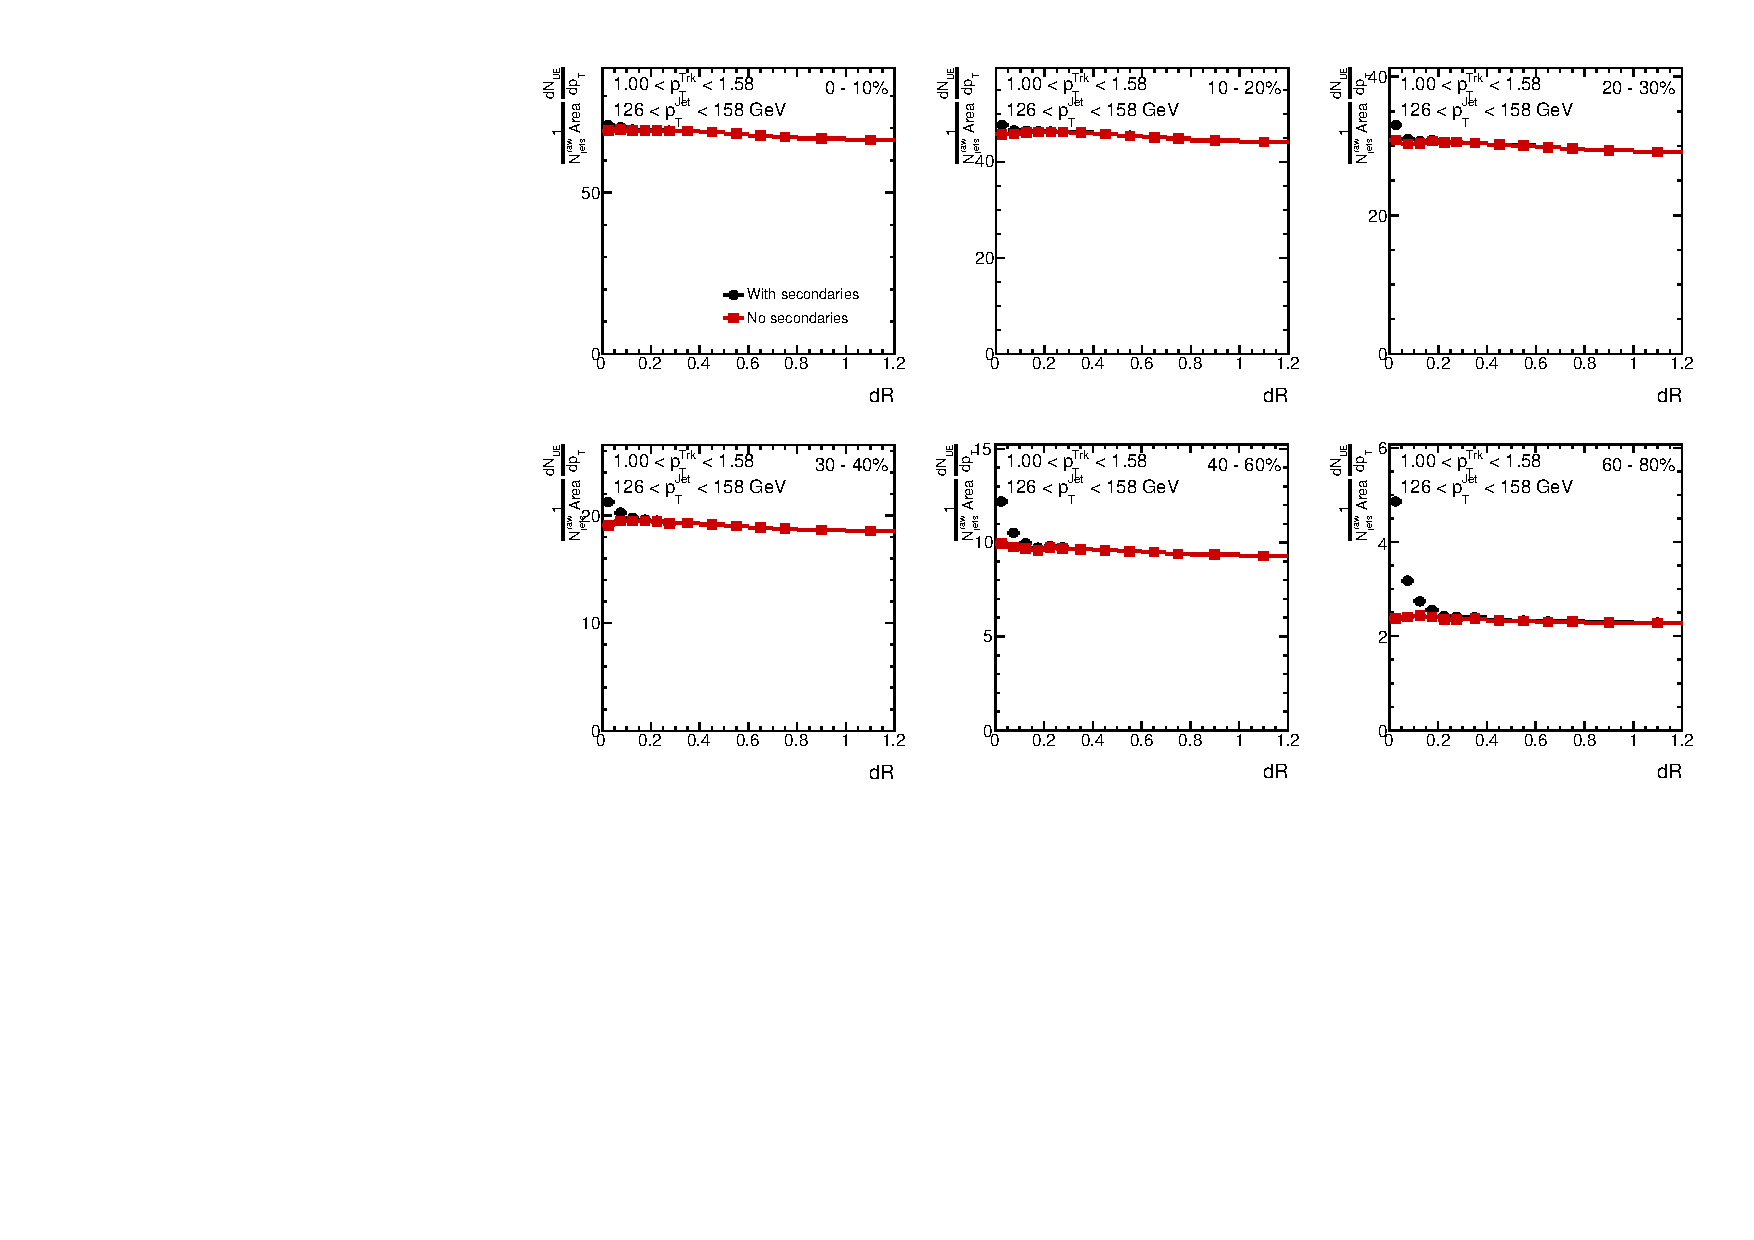
\includegraphics[width=0.9\textwidth]{figures/main/UE/UE_v_dR_pt1GeV.pdf}
\caption{UE estimated from tracks which do not have an associated truth particle in jet with \pt\ from 126 to 158 GeV and for the lowest track \pt\ interval (1--1.58 GeV).
The two different distribution shows the UE with and without the contribution from the secondary particles.}
\label{fig:UEdR}
\end{figure}   

%%%%%%%%%%%%%%%
\subsubsection{Cone Method}
\label{sec:cone_method}
The cone method uses a regular grid of 9 cones of size $R = 0.8$ covering the full inner detector region (shown in Figure~\ref{fig:cone_grid}).
The size of the cone corresponds to the radial phase space being investigated (0.8 in this case).
Cones within a distance of $dR=1.6$ to a reconstructed jet are excluded if $\ptjet > 90$ GeV.
They are also excluded if they contain a track with $\pt > 10$ GeV.
The 10 GeV was cut was chosen based on the small centrality dependence of the combined rate of fake and underlying event tracks above 10 GeV as shown in Figure~\ref{fig:fakeratehijing}.
The fraction of events as a function of number of cones used in each centrality bin is shown in Figure~\ref{fig:cone_stats}.
It can be seen that in the MC the number of cones used is consistent with there being no jet quenching.
This is as expected since the jets in the \pbpb\ MC overlay are coming from \pythia\ and are unquenched.
Moreover, quenching in central \pbpb\ data leads to only one jet causing exclusions, consistent with most events using 7 cones.
For more peripheral \pbpb\ collisions, the cone distribution tends to look like the distribution with no quenching.

\begin{figure}
\centering
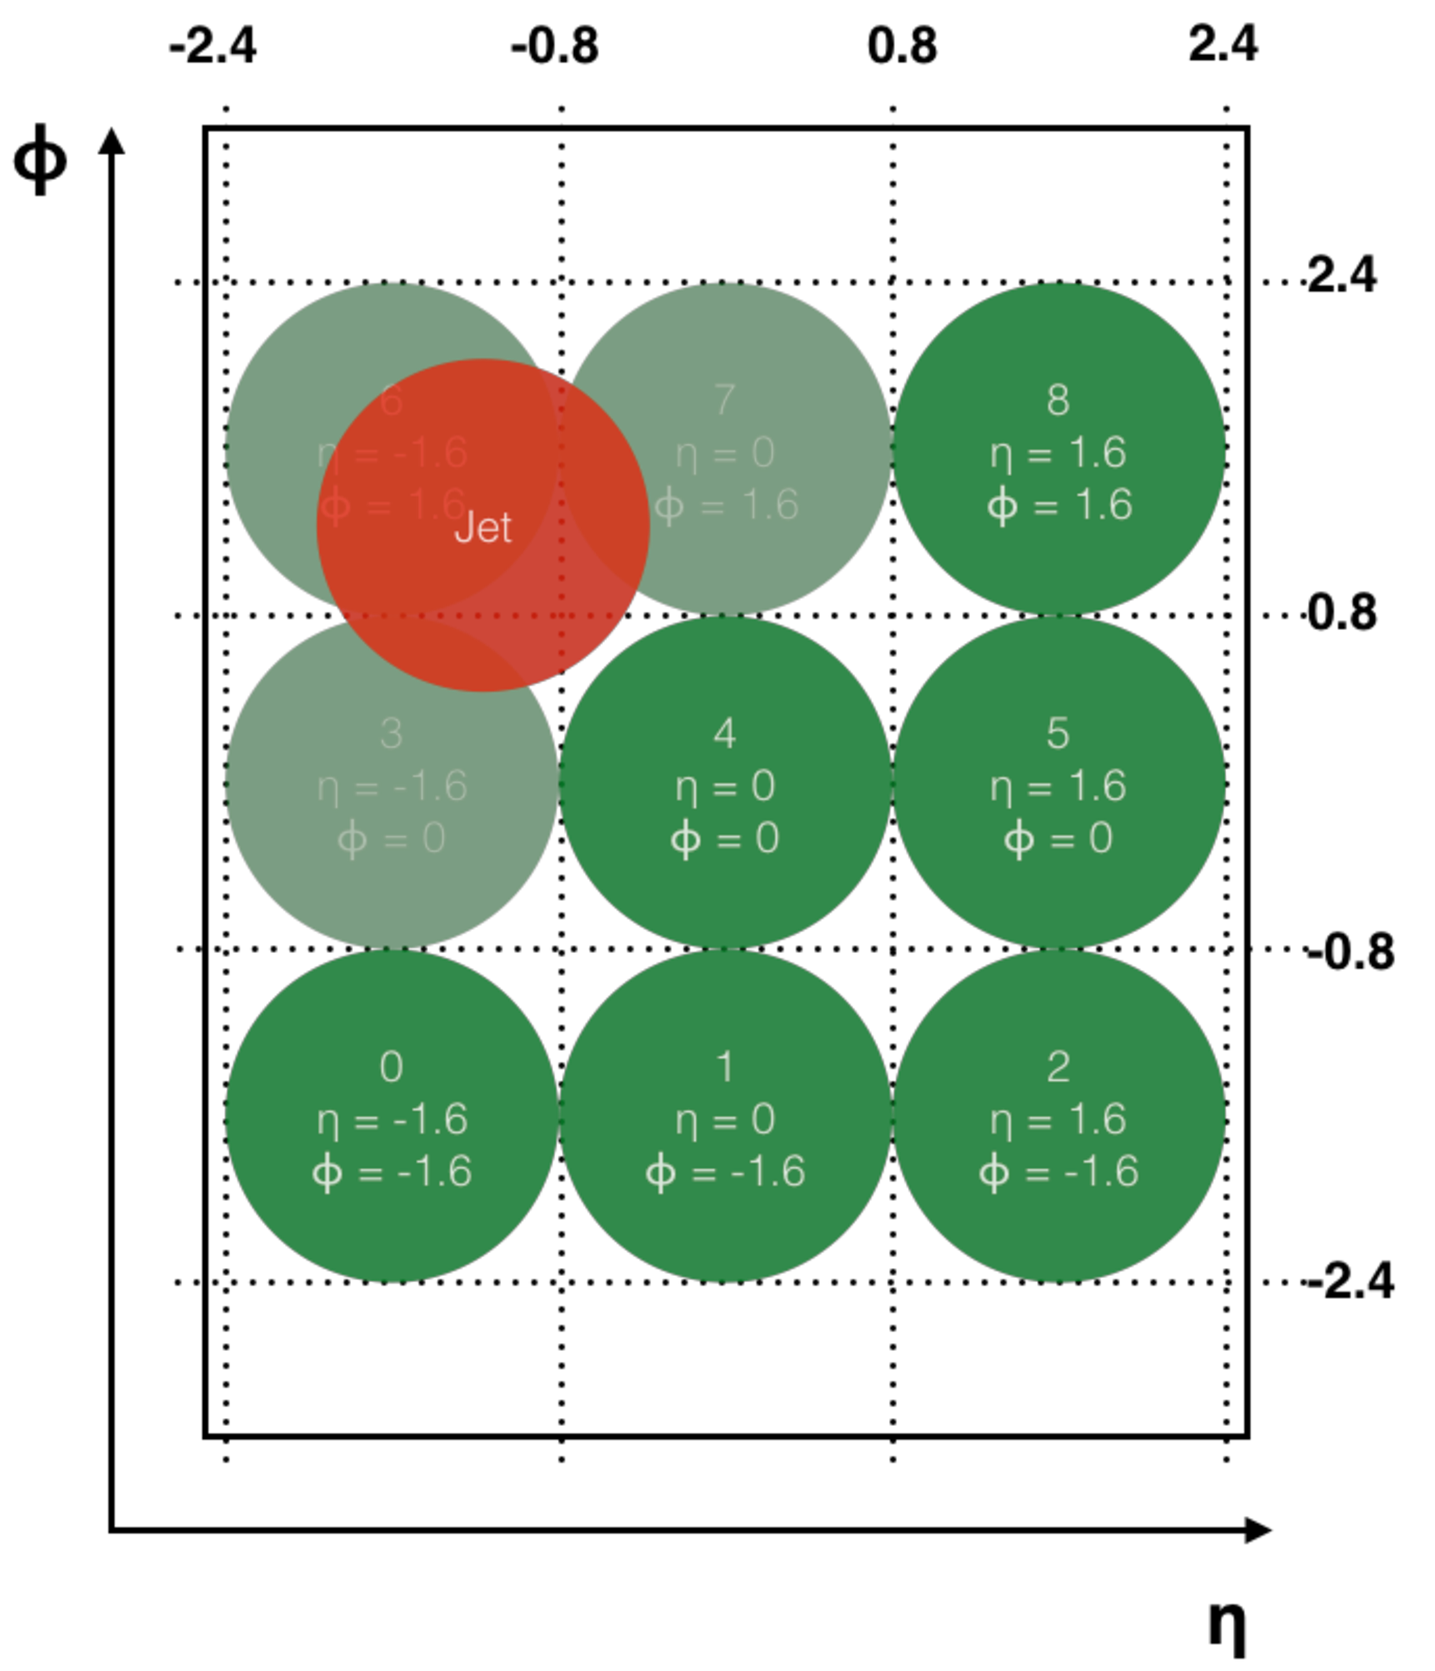
\includegraphics[width=0.45\textwidth]{figures/main/UE/cone_grid.pdf}
\caption{Illustration of the cone method to estimate the underlying event.
Cones numbered 3, 6, and 7 are excluded based based on the jet shown in red.}
\label{fig:cone_grid}
\end{figure}   

\begin{figure}
\centering
\includegraphics[width=0.9\textwidth]{figures/main/UE/cone_stats}
\caption{Fraction of events as a function of the number of cones used for the estimation of the underlying event.}
\label{fig:cone_stats}
\end{figure}   

The resulting UE charged particle yields $\fd \nchUE^{\mathrm{Cone}}/ \fd \pTch$ are evaluated over the 1 -- 10 GeV range as a function of \pt\, \ptjet\, centrality, and \rvar, and then averaged over all cones according to.

\begin{eqnarray}
\frac{\fd n_{\mathrm{ch}}^{\mathrm{UE Cone}}}{\fd \pTch}  = \frac{1}{N_{\mathrm{cones}}} \frac{1}{\varepsilon} \frac{\Delta N^{\mathrm{cone}}_{\mathrm{ch}} (\pTch, \ptjet, \etajet)}{\Delta \pTch}
\end{eqnarray}
Here $N_{\mathrm{cones}}$ is the number of background cones associated with a given jet with \ptjet.
$\Delta N^{\mathrm{cone}}_{\mathrm{ch}}$ is the number of charged particles summed across all background cones associated to the jet in question.
The cone method estimates the UE yields only from events containing jets included in the analysis, ensuring that the background automatically had the correct distribution of centralities within a given centrality bin.

The UE contribution as measured using the cone method in data needs to be further corrected for three effects:

\paragraph{Correction for $\eta$-dependence:}
To account for differences in the yields of UE particles at the position of the jet and at the position of the track for the random cone entering the UE estimate, the $\eta$ distribution of charged particles from MC overlay events is used to appropriately weigh the UE tracks.
The correction is then the ratio of the value of the $\fd \nch / \fd\eta$ at the position of the jet and the track.
The impact of the correction in 0-10\% \pbpb\ collisions is shown in Figure~\ref{fig:eta_corr}

%\begin{figure}
%\centering
%\includegraphics[width=0.45\textwidth]{figures/main/UE/eta_correction.pdf}
%\caption{Ratio of the $\NchUECone$ distributions with and without the correction for $\eta$ dependence in the most central 0-10\% \pbpb\ collisions, evaluated with a subset of the data (70k events).
%Figure taken from Ref.~\cite{Sickles:2235420}.}
%\label{fig:eta_corr}
%\end{figure}


\paragraph{Correction for flow:}
Elliptic flow is the characteristic sinusoidal modulation of the yields of particles along the azimuth in heavy ion collisions.
The maximum amplitude of the modulation determines the reaction plane, with more momenta being measured in plane than out of plane.
Ref.~\cite{Aaboud:2018ves} provides a basic measurement of the magnitude of the elliptic flow, and its \pt\ dependence.
The correction for this effect was based on a parametrization of the \pTch and centrality dependence of previously measured elliptic flow coefficients, $v_{2}$ \cite{Aaboud:2018ves}.
The reaction plane angle $\Psi$ is estimated on an event-by-event basis by using the $\phi$ variation of transverse energy in the forward calorimeter.
The correction factor is evaluated as a function of the distance of the jet from the reaction plane $\cos2(\phijet - \Psi)$.
The correction is less (greater) than unity for jets in a direction perpendicular (parallel) to the reaction plane.
Jets perpendicular (parallel) to the plane typically have a lower (higher) UE, and a cone at a random position in the ID is corrected down (up).
The size of the correction is at the level of a few percent, and decreases with increasing track \pt, as is shown in Figure~\ref{fig:flow_corr}


\begin{figure}
\begin{subfigure}{0.5\textwidth}
\centering \includegraphics[width=1\textwidth]{figures/main/UE/eta_correction.pdf}
\caption{}
\label{fig:eta_corr}
\end{subfigure}
\begin{subfigure}{0.5\textwidth}
\centering \includegraphics[width=1\textwidth]{figures/main/UE/flow_correction.pdf}
\caption{}
\label{fig:flow_corr}
\end{subfigure}
\caption{Ratio of the $\NchUECone$ distributions with and without the correction for (left) $\eta$ dependence and (right) elliptic flow in the most central 0-10\% \pbpb\ collisions, evaluated with a subset of the data (70k events).
Figures taken from Ref.~\cite{Sickles:2235420}.}
\label{fig:cone_corrections}
\end{figure}



%\begin{figure}
%\centering
%\includegraphics[width=0.45 \textwidth]{figures/main/UE/flow_correction.pdf}
%\caption{Ratio of the $\NchUECone$ distributions with and without the correction for elliptic flow in the most central 0-10\% \pbpb\ collisions, evaluated with a subset of the data (70k events).
%Figure taken from Ref.~\cite{Sickles:2235420}.}
%\label{fig:flow_corr}
%\end{figure}

\paragraph{UE and JER correlation:}
The interplay between the UE and the JER will be described here is discussed in further detail in Ref.~\cite{ATLAS-COM-PHYS-2012-1653}.
Due to the steeply falling nature of the jet \pt\ spectra, the smearing due to jet energy resolution leads to a net migration of jets from lower \pt\ to higher \pt\ values (hereafter referred to as ``up-feeding'') such that a jet reconstructed with a given \pTrec\ will correspond, on average, to a lower truth jet \pT, \avgpttrue.
The up-feeding was observed to induce in the MC a difference between the UE yields determined using the MC overlay events and the actual UE contribution to reconstructed jets.
The magnitude of this difference was found to be centrality dependent and exhibited a weak \pTjet\ dependence.
That difference was found to result from intrinsic correlations between the UE contribution to the yield of particles measured inside the jet and the MC \pTjet\ shift, $\Delta p_{\mathrm{T}}^{\mathrm{jet}}= \pTrec - \pTtrue$.
In particular, jets with positive (negative) $\Delta p_{\mathrm{T}}^{\mathrm{jet}}$ were found to have an UE contribution larger (smaller) than jets with $\Delta p_{\mathrm{T}}^{\mathrm{jet}} \sim 0$.

To correct for this effect, the centrality-, $\pTjet$-, $r-$ and $\pTch$-dependent multiplicative correction factors were applied on $\fd \nchUE^{\mathrm{Cone}}/ \fd \pTch$ distributions.
These multiplicative factors, $w_{\mathrm{UE}}$, were estimated as a ratio of UE distributions calculated in MC samples using the "Map method", $\Dptr_{f}$, and the "Cone Method".

\begin{eqnarray}
w_{\mathrm{UE}} (\pT) = \frac{\fd \nchUE^{\mathrm{Map}}/ \fd \pTch}{\fd \nchUE^{\mathrm{Cone}}/ \fd \pTch}\bigg|_{\mathrm{MC}}
\end{eqnarray}   
Examples of these factors are shown in Figure~\ref{fig:UEweights}.
The correction by construction corrects also for fakes and secondary contribution in the track \pT\ region 1-10~GeV in \PbPb\ collisions.
%These factors are also shown in Figure~\ref{fig:UEweights_r_jet0}, as a function of \rvar\ for different track \pt\ bins, for $126 < \ptjet\ < 158 \GeV$.
The size of these corrections integrated over $\rvar = 0.4$ is comparable to the UE-JER correction done in \cite{PhysRevC.98.024908}.

\begin{figure}
\centering
\begin{subfigure}{1.\textwidth}
\centering \includegraphics[page=2,width=1.\textwidth]{figures/main/UE/UE_factors.pdf}
\caption{}
\label{fig:UEweights_r2}
\end{subfigure} \\
\begin{subfigure}{1.\textwidth}
\centering \includegraphics[page=6,width=1.\textwidth]{figures/main/UE/UE_factors.pdf}
\caption{}
\label{fig:UEweights_r6}
\end{subfigure}
\caption{The multiplicative correction factors that correct for the correlation between the UE and the JER, fake and secondary particles in different centrality classes and \mbox{$ 0.05 < r < 0.10$} (top) and \mbox{$ 0.25 < r < 0.30$ (bottom)}.}
\label{fig:UEweights}
\end{figure}

%\begin{figure}
%\centering
%\includegraphics[page=1,width=1.\textwidth]{figures/main/UE/UE_factors_r.pdf} \\
%\caption{The multiplicative correction factors that correct for the correlation between the UE and the JER, fake and secondary particles in different centrality classes, as a function of $r$ for $126 < \ptjet < 158 \GeV$.}
%\label{fig:UEweights_r_jet0}
%\end{figure}


The absolute magnitude of the correction increases towards the higher track \pt\ in the jet core where the UE is smaller.
This behavior has two contributions: the intrinsic correlations between the UE contribution to the yield of particles measured inside the jet and the MC \pTjet\ shift as it was discussed earlier, and the correlation of production of secondary particles with the jet.
The production of secondary particles is associated with presence of primary particles.
Thus, the production of secondary particles is enhanced in the jet due to the higher density of primary particles compared to the regions outside a jet.
This was shown in Figure~\ref{fig:UEdR} where the UE evaluated in term of particles without matching to truth particles in MC with and without the contribution from secondary particles is presented and where the yield of secondary particles is significant only at smaller $dR$, that is, within a jet.
Figure~\ref{fig:UEdR} also shows that the relative yield of secondary particles to the yield of the UE particles is increasing with decreasing collisions centrality.
Furthermore, the relative contribution of secondary particles to the UE increases with the track \pT\ as the fraction of the secondary particles decreases only slowly with the increasing track \pT\ (Figure~\ref{fig:fakeratepbpb}), however, the UE decreases strongly with the increasing track \pT\ (Figure~\ref{fig:UEimpact}).
This results in lower UE contribution estimated using the MB collisions where tracks are not associated to a jet.


As shown in Figure~\ref{fig:conemethod_mapmethod}, the two UE estimation methods give almost identical UE at angles outside the $R=0.4$ jet as the role of the two effects discussed here decreases.
The difference between the methods varies slowly with \ptjet\ and track \pT, with a small centrality dependence coming from fact that the underlying event strongly depends on the centrality.

\begin{figure}
\centering
\includegraphics[page=2,width=1.\textwidth]{figures/main/UE/UE_x_ratio_c0}
\caption{The difference between the cone method and the map method as a function for \rvar\ for 0-10\% \pbpb\ collisions, in 126-158 GeV jets, 1-1.6 GeV tracks.}
\label{fig:conemethod_mapmethod}
\end{figure}


For $\pt > 10$ GeV and in  \pp\ system fake contribution is corrected as described at the beginning of Section~\ref{sec:trackreco}.
The corrected UE distributions, $\fd \cnchUE / \fd \pTch$ are then subtracted from measured distributions as follows

\begin{eqnarray}
\frac{\fd n_{\mathrm{ch}}^{\mathrm{sub}}}{\fd \pTch}  = \frac{\fd n_{\mathrm{ch}}^{\mathrm{meas}}}{\fd \pTch} - {w_{\mathrm{UE}} (\pT)} \left( \frac{\fd \nchUE^{\mathrm{Cone}}}{\fd \pTch} \bigg|_{\mathrm{Data}} \right)  = \frac{\fd n_{\mathrm{ch}}^{\mathrm{meas}}}{\fd \pTch} - \frac{\fd \cnchUE}{\fd \pTch}
\end{eqnarray}


The impact of the underlying event and fake track subtraction on the \Dptr\ distributions is shown in Figure~\ref{fig:UEimpact}.
The magnitude of this correction is the largest for low track \pt\ in central \pbpb\ collisions and the largest annulus.
In the most extreme case the S/B ratios can be as low as 1/100.
The size of the correction decreases rapidly with increasing track \pt, decreasing centrality and towards the core of the jet.
In \pp\ collisions the magnitude of the fake track subtraction is always much less than 5\%.

\begin{figure}
\begin{subfigure}{0.5\textwidth}
\centering \includegraphics[page=2,width=1\textwidth]{figures/main/UE/ChPS_B2S_PbPb_data.pdf}
\caption{}
\label{fig:UEimpact_r2}
\end{subfigure}
\begin{subfigure}{0.5\textwidth}
\centering \includegraphics[page=4,width=1\textwidth]{figures/main/UE/ChPS_B2S_PbPb_data.pdf}
\caption{}
\label{fig:UEimpact_r4}
\end{subfigure} \\
\begin{subfigure}{0.5\textwidth}
\centering \includegraphics[page=6,width=1\textwidth]{figures/main/UE/ChPS_B2S_PbPb_data.pdf}
\caption{}
\label{fig:UEimpact_r6}
\end{subfigure}
\begin{subfigure}{0.5\textwidth}
\centering \includegraphics[page=10,width=1\textwidth]{figures/main/UE/ChPS_B2S_PbPb_data.pdf}
\caption{}
\label{fig:UEimpact_r10}
\end{subfigure}
\caption{Ratio between the raw \Dptr\ distributions before and after the UE  subtraction in different centrality classes and different jet \pT\ intervals for different distances from the jet axis: $0.05 < r < 0.10$, $0.15 < r < 0.20$, $0.25 < r < 0.30$, $0.60 < r < 0.70$.}
\label{fig:UEimpact}
\end{figure}


The basic performance of the UE subtraction was tested in the MC overlay dataset.
This closure test was performed using the MC overlay sample that has the same UE as in the data and will be discussed in the next subsection.
The truth \Rdptr\ distributions were compared to fully corrected \Rdptr\ distributions where the UE contribution is subtracted by the same method as used in the data (see Figure~\ref{fig:PbPb_ChPS_closure}).
From the above mentioned tests we concluded that the UE subtraction procedure is correct and works well.
The UE estimate is subjected to a variation as part of the systematic uncertainties.
For the \pp\ data, we have not performed any UE subtraction.



%%%%%%%%%%%%%%%%%%%%%%%%%%%%%%
\subsection{Unfolding}
\label{sec:unfolding}

Unfolding procedures are used to remove Instrumental effects like detector resolutions and allow for direct comparisons to theory calculations \cite{DAgostini:1994zf}.
This is done via the approach based on Bayes theorem that is implemented in the RooUnfold package and uses ``response matrices'' \cite{Adye:2011gm}.
These matrices are multidimensional object that created using the MC and describe the migration between the reconstructed quantities and the corresponding truth quantities that are to be unfolded.

This analysis uses three separate unfolding procedures that are discussed in this section.

\begin{itemize}
\item One dimensional unfolding for the \ptjet\ spectra for the normalization.
\item Two dimensional Bayesian unfolding in \pttrk\ and \ptjet for jet \pt\ dependent yields of charged particles.
\item Bin by bin correction for the jet and track position resolution.
\end{itemize}

To achieve better correspondence with the data, the response matrices for both the one and two dimensional unfolding are reweighted so that the distributions match the shapes in the reconstructed data.

\subsubsection{One Dimensional Unfolding for Jet Spectra}
\label{sec:1dunfolding}
The charged particle spectra need to be normalized by the number of jets in given jet \pt\ interval.
Thus, the jet spectra needs to be corrected for bin migration due to the finite JER by unfolding procedure.
The unfolding is done via a one dimensional Bayesian unfolding procedure with 4 iterations implemented as part of the RooUnfold~\cite{Adye:2011gm} package.
The \pp\ and \PbPb\ MC samples are used to construct two dimensional response matrices in terms of \ptjettruth\ and \ptjetreco.
These matrices can be seen in Figure~\ref{fig:jetspect_respmatrix} and are evaluated separately for \pp\ and in different centrality intervals for \PbPb\ collisions.
The technical closure of this unfolding procedure (done using un-reweighted response matrices to unfold the reconstructed jet spectra) is shown in Figure~\ref{fig:jetspect_closure}, as a function of \ptjet\ for jets in the $|y| < $ 1.7 region.
A good recovery of the truth distribution is seen for both 1\% for \pbpb\ and \pp\ MC samples.


\begin{figure}
\begin{subfigure}{0.7\textwidth}
\centering
\includegraphics[page=5, width=1\textwidth]{figures/main/corrections/resp_matrix_jet_PbPb_MC.pdf}
\caption{}
\label{fig:PbPb_jetspect_respmatrix}
\end{subfigure} 
\begin{subfigure}{0.30\textwidth}
\centering
\includegraphics[page=5, width=1\textwidth]{figures/main/corrections/resp_matrix_jet_pp_MC.pdf}
\caption{}
\label{fig:pp_jetspect_respmatrix}
\end{subfigure}
\caption{The response matrices in terms of \ptjetreco\ and \ptjettruth\ in the jet $|y| < $1.7 region, in (left) data overlay \pbpb\ MC samples, with each panel being a different centrality bin and (right) in \pp\ MC samples.}
\label{fig:jetspect_respmatrix}
\end{figure}



\begin{figure}
\begin{subfigure}{0.7\textwidth}
\centering
\includegraphics[page=5, width=1\textwidth]{figures/main/corrections/spect_closure_PbPb_MC.pdf}
\caption{}
\label{fig:PbPb_jetspect_closure}
\end{subfigure} 
\begin{subfigure}{0.30\textwidth}
\centering
\includegraphics[page=5, width=1\textwidth]{figures/main/corrections/spect_closure_pp_MC.pdf}
\caption{}
\label{fig:pp_jetspect_closure}
\end{subfigure}
\caption{The jet spectra and MC closure as a function of \ptjet\ in the jet $|y| < $1.7 region, in (left) data overlay \pbpb\ MC samples, with each panel being a different centrality bin and (right) in \pp\ MC samples.
The closure is seen to be well within 1\%.}
\label{fig:jetspect_closure}
\end{figure}


\subsubsection{Two Dimensional Unfolding for Charged Particle Spectra}
\label{sec:2dunfolding}


The observed correlation between the jet response in the detector and the jet fragmentation necessitates a two dimensional unfolding~\cite{PhysRevC.98.024908}.
For example, gluon jets, which have in general a softer fragmentation function, are observed to have a lower energy response than quark jets~\cite{Aad:2014bia}.
%The Global Sequential Calibration to the \pp\ jet collections~\cite{ATLAS:2015oia}, reduces the fragmentation dependence to the JES, but these calibrations are not available for the HI jet collections used in this analysis.
We use the RooUnfold~\cite{Adye:2011gm} implementation of the two dimensional iterative Bayesian unfolding~\cite{D'Agostini:1994zf} with 4 iterations.
The MC \pbpb\ and \pp\ samples are used to construct a 4-dimensional response matrix in \pttrktruth, \ptjettruth, \pttrkreco, and \ptjetreco, shown in Figure~\ref{fig:ChPS_respmatrix}.
The response matrix $A_{ijkl}$ describes the probability that an event from the truth track \pt\  bin $j$ and truth jet \pT\ bin $l$ is found in reconstructed bin $i$,$k$:

\begin{equation}
\mu_{jl} = \sum_{i,k} A_{ijkl}x^{\text{truth}}_{jl}.
\end{equation} 


\begin{figure}
\begin{subfigure}{0.7\textwidth}
\centering
\includegraphics[page=5, width=1\textwidth]{figures/main/corrections/resp_matrix_ChPS_PbPb_MC.pdf}
\caption{}
\label{fig:PbPb_ChPS_respmatrix}
\end{subfigure} 
\begin{subfigure}{0.30\textwidth}
\centering
\includegraphics[page=5, width=1\textwidth]{figures/main/corrections/resp_matrix_ChPS_pp_MC.pdf}
\caption{}
\label{fig:pp_ChPS_respmatrix}
\end{subfigure}
\caption{The response matrices in terms of \ptjetreco, \ptjettruth, \pttrkreco, and \pttrktruth, for reconstructed track - reconstructed jet pairs, that have 0.20 $< r < $0.25, in (left) data overlay \pbpb\ MC samples, with each panel being a different centrality bin and (right) in \pp\ MC samples.}
\label{fig:ChPS_respmatrix}
\end{figure}


\subsubsection{Bin-by-bin correction for Angular resolution}
\label{sec:bbbcorrection}

There is an additional unfolding procedure applied in this analysis to correct for the jet and the track position resolution that results in the migration in angular distance $r$.
The migration is dominated by the poor jet angular resolution (shown in Figure~\ref{fig:jet_posResolution}), since the track angular resolution shown in Figure~\ref{fig:trk_posResolution} is very good.

\begin{figure}
\begin{subfigure}{.5\textwidth}
\centering \includegraphics[width=1.\textwidth]{figures/main/corrections/trk_res_eta_ppTight.pdf}
\caption{}
\end{subfigure}
\begin{subfigure}{.5\textwidth}  
\centering \includegraphics[width=1.\textwidth]{figures/main/corrections/trk_res_phi_ppTight.pdf}
\caption{}
\end{subfigure}
\caption{The (left) $\eta$ and (right) $\phi$ position resolution of the tracker as a function of \pttruth\ for different centrality and $\eta$ regions in \pbpb\ MC overlay samples.
The different curves are different centralities, and it can be seen that there is no centrality dependence.}
\label{fig:trk_posResolution}
\end{figure}

The correction factors are derived using response matrices that correlate the reconstructed and truth angular distance $r$.
These matrices are evaluated for different jet and track \pT\ in different centrality classes.
Examples of the response matrices are shown in Figure~\ref{fig:bbb_2d_response} for \pbpb\ and \pp\ MC samples.
The bin-by-bin correction procedure is applied to \Dptr\ distribution unfolded to the particle level in terms of track and jet \pT\ by the two unfolding procedures discussed above.
The correction factors for angular resolution were derived using the the reconstructed jets and tracks where the reconstructed jet and track \pT\ is replaced by the corresponding truth \pT.
The bin-by-bin factors are then estimated as ratio of projections from the response matrices on the truth and reconstructed axis.
These correction factors are shown in Figure~\ref{fig:pos_corr_factors} for \pbpb\ and \pp\ collisions as a function of \rvar.
The efficiency and purity are a measure of what fraction of jets are reconstructed in the same bin as their generator level counterpart.
The efficiency is given by the fractional distribution of reconstructed jets at a fixed truth \ptjet\ while the purity is given by the fractional distribution of truth jets at a fixed reconstructed \ptjet.
These are shown in the Figures~\ref{fig:RespEfficiencyPurity}.


\begin{figure}
\centering
\begin{subfigure}{1.\textwidth}
\centering \includegraphics[page=1, width=1\textwidth]{figures/main/corrections/ShapeResponse2D_PbPb.pdf}
\caption{}
\label{fig:PbPb_bbb_2d_response}
\end{subfigure} \\
\begin{subfigure}{1.\textwidth}
\centering \includegraphics[page=1, width=1\textwidth]{figures/main/corrections/ShapeResponse2D_pp.pdf}
\caption{}
\label{fig:pp_bbb_2d_response}
\end{subfigure}
\caption{The response matrix for the bin by bin correction applied to the unfolded charged particle spectra.
This accounts for the jet position resolution.
Each panel is a different \pttrk\ bin, for $126 < \ptjet\ < 158$ GeV jets, in (top) central collisions from \pbpb\ MC overlay samples and (bottom) \pp\ MC samples.}
\label{fig:bbb_2d_response}
\end{figure}


\begin{figure}
\centering
\begin{subfigure}{1.\textwidth}
\centering \includegraphics[page=1, width=1\textwidth]{figures/main/corrections/RatioProj_PbPb}
\caption{}
\label{fig:pos_corr_factors_PbPb_c0}
\end{subfigure} \\
\begin{subfigure}{1.\textwidth}
\centering \includegraphics[page=1, width=1\textwidth]{figures/main/corrections/RatioProj_pp}
\caption{}
\label{fig:pos_corr_factors_pp}
\end{subfigure}
\caption{The correction factors applied to the unfolded charged particle spectra, as a function of $r$, with each panel showing a different track \pt\ bin, and each curve showing a different \ptjet\ range, in (top) central collisions from \pbpb\ MC overlay samples and (bottom) \pp\ MC samples.} 
\label{fig:pos_corr_factors}
\end{figure}


\begin{figure}
\centering
\begin{subfigure}{1.\textwidth}
\centering \includegraphics[page=1, width=1\textwidth]{figures/main/corrections/RespPurity_PbPb}
\caption{}
\label{fig:RespPurity_PbPb}
\end{subfigure}
\begin{subfigure}{1.\textwidth}
\centering \includegraphics[page=1, width=1\textwidth]{figures/main/corrections/RespEfficiency_PbPb}
\caption{}
\label{fig:RespEfficiency_PbPb}
\end{subfigure}
\caption{The (top) purity and (bottom) efficiency of the bin-by-bin unfolding factors used to correct for the angular resolution for different \pttrk\ ranges tracks (in different panels), shown as a function of \rvar\ for different \ptjet\ ranges, in the most central 0--10\% \pbpb\ collisions.}
\label{fig:RespEfficiencyPurity}
\end{figure}


The robustness of this correction can be validated by constructing \Dptr\ distributions using a coarser \pt\ binning (entire analysis chain is re-done) and comparing them to a summation of the individually unfolded narrow bins.
This comparison can be seen in Figure~\ref{fig:MergedBinCheck}, for $1 < \pt < 4$ GeV, $126 < \ptjet < 158$ GeV,  for 0-10\%.
central \pbpb\ and \pp\ collisions, and is seen to be unity.

\begin{figure}
\centering
\includegraphics[width=0.7\textwidth]{figures/main/general/MergedBinCheck.pdf}
\caption{The \Dptr\ distributions in \pp\ and 0--10\% central \pbpb, constructed using a single bin from 1--4 GeV (merging the first three \pt\ bins in this analysis) compared to the \Dptr\ distributions constructed by adding up the bins individually: \mbox{1--1.6 GeV}, \mbox{1.6--2.5 GeV} and \mbox{2.5--4 GeV}.
This comparison tests the robustness of the angular bin by bin correction and its dependence on the width of the \pt\ bins.}
\label{fig:MergedBinCheck}
\end{figure}


It can be seen that these corrections become large at the edges of the jet cone for tracks that carry a significant fraction of the jet momentum.
This is an artifact of the jet reconstruction algorithm, where a truth track near the edge of a truth jet will pull the reconstructed jet towards itself, causing a depletion of high \pt\ particles at the edge of the jet cone.
This depletion can be seen in the distribution of truth charged particles in truth jets shown in Figure~\ref{fig:truthProj_pp} and was also seen in Ref.~\cite{Choudalakis:1248716}.
These large factors result in a large non-closure near the jet edge for tracks carrying a significant momentum fraction of the jet.
To exclude these effects, the results are only shown for tracks that show a closure of less than 5\%.

\begin{figure}
\centering
\includegraphics[page=1, width=1\textwidth]{figures/main/corrections/TruthProj_pp}
\caption{The distribution of truth charged particles in truth jets for different track \pt\ ranges and \ptjet\ ranges in \pp\ collisions.
It can be seen that there is a kink in the distribution at the jet edge for high \pt\ tracks.}
\label{fig:truthProj_pp}
\end{figure}


The \Dptr\ distributions at various stages of the analysis in \pp\ and \pbpb\ MC and data are shown in Figure~\ref{fig:evol_pp} and Figure~\ref{fig:evol_PbPb}.

\begin{figure}
\begin{subfigure}{0.5\textwidth}
\centering \includegraphics[page=5, width=1\textwidth]{figures/main/corrections/evol_pp_MC.pdf}
\caption{}
\end{subfigure}
\begin{subfigure}{0.5\textwidth}
\centering \includegraphics[page=5, width=1\textwidth]{figures/main/corrections/evol_pp_data.pdf}
\caption{}
\end{subfigure}
\caption{The evolution of the \Dptr\ distributions for \pp\ MC (left) and data (right) as various corrections are applied.
The spectra is shown for tracks with $0.05 < \Delta r < 0.10$ away from the jet axis, for $126 < \ptjet < 158$ GeV.
The ratios showing the effect of the unfolding and bin by bin corrections (left and right), as well as the MC closure (left) are shown in the lower half of the panels.}
\label{fig:evol_pp}
\end{figure}


\begin{figure}
\centering
\begin{subfigure}{0.9\textwidth}
\centering \includegraphics[page=5, width=1\textwidth]{figures/main/corrections/evol_PbPb_MC.pdf}
\caption{}
\end{subfigure}
\begin{subfigure}{0.9\textwidth}
\centering \includegraphics[page=5, width=1\textwidth]{figures/main/corrections/evol_PbPb_data.pdf}
\caption{}
\end{subfigure}
\caption{The evolution of the \Dptr\ distributions for \PbPb\ MC (top) and data (bottom) as various corrections are applied.
The spectra is shown for tracks with $0.05 < \Delta r < 0.10$ away from the jet axis, for $126 < \ptjet < 158$ GeV.
The ratios showing the effect of the subtraction, unfolding and bin by bin correction as well as the comparison to truth are shown in the lower half of each panel.
The different panels are different centrality selections.}
\label{fig:evol_PbPb}
\end{figure}


The MC closure of the charged particle spectra as a function of \pt\ in \pp\ MC and \pbpb\ MC overlay samples can be seen in Figures~\ref{fig:ChPS_closure} and is well within 1\% for low \pt\ particles.


\begin{figure}
\begin{subfigure}{0.7\textwidth}
\centering
\includegraphics[page=5, width=1\textwidth]{figures/main/corrections/ChPS_final_PbPb_MC.pdf}
\caption{}
\label{fig:PbPb_ChPS_closure}
\end{subfigure} 
\begin{subfigure}{0.30\textwidth}
\centering
\includegraphics[page=5, width=1\textwidth]{figures/main/corrections/ChPS_final_pp_MC.pdf}
\caption{}
\label{fig:pp_ChPS_closure}
\end{subfigure}
\caption{The response matrices in terms of \ptjetreco\ and \ptjettruth\ in the jet $|y| < $1.7 region, in (left) \pbpb\ MC overlay with each panel being a different centrality bin and (right) in \pp\ MC.}
\label{fig:ChPS_closure}
\end{figure}






\section{Systematic Uncertainties}
\label{sec:systematic}
% !TEX encoding = UTF-8 Unicode
% !TEX root = thesis-ex.tex

This section gives an overview of the sources of systematic uncertainties on the \pp\ and \pbpb\ charged particle spectra associated with jet.
These include:

\begin{itemize}
\item Jet energy scale
\item Jet energy resolution
\item Tracking selections
%\item Truth track definition
%\item Detector material description in simulation
%\item Tracking in dense environments
%\item Fake track subtraction
%\item Track momentum
\item Unfolding
\item Underlying event contribution
\item MC non-closure
\end{itemize}

The systematic uncertainties are evaluated separately for \Dptr\ distributions and for their ratios as a function of jet \pT\ for \pp\ and \pbpb\ collisions.
For each systematic variation, the entire analysis procedure is repeated to ensure that the jets are treated in a consistent manner throughout the analysis.
The positive relative shift was used to calculate the upper bound of the systematic uncertainty, whereas the negative relative shift was used to calculate the lower bound.
All uncertainties except the unfolding and the MC non-closure are assumed to be correlated and are evaluated by comparing the \Rdptr\ distributions for the various systematic variations to the nominal \Rdptr\ distribution.
For uncorrelated systematic uncertainties, the uncertainty on the \RDptr\ distribution is evaluated by adding the uncertainties on the \pp\ and \pbpb\ \Dptr\ distributions in quadrature.
The total systematic uncertainties on the \Rdptr\ distributions for a selection of track \pt\ ranges (1.0--1.6 \GeV, 2.5--4.0 \GeV, 6.3--10 \GeV) in jets with \pt\ in the 126--158 \GeV\ range are shown in Figures~\ref{fig:rdptr_sys_uncert1} and \ref{fig:rdptr_sys_uncert2}. 
% Figure~\ref{fig:rdptr_sys_uncert1}-\ref{fig:rdptr_sys_uncert2}.
%The systematic uncertainties for other jet \pT\ intervals as show in appendix \ref{sec:appendixA}.



\begin{figure}
\centering
\begin{subfigure}[b]{\textwidth}
    \centering
    \includegraphics[page=1, width=\textwidth]{figures/main/systematics/Summary_ChPS_dR_sys_PbPb_error}
    \caption{}
    \label{fig:rdptr_sys_uncert1a}
\end{subfigure} \\
\begin{subfigure}[b]{\textwidth}
    \centering
    \includegraphics[page=3, width=\textwidth]{figures/main/systematics/Summary_ChPS_dR_sys_PbPb_error}
    \caption{}
    \label{fig:rdptr_sys_uncert1b}
\end{subfigure}\hfill
   \caption{A summary of the systematic uncertainties on \RDptr\ distributions for different track \mbox{$1.0 < \pt < 1.6$ GeV} (top) and \mbox{$2.5 < \pt < 4.0$ GeV} (bottom), for jets with \pt\ 126--158 \GeV, as a function of \rvar\ for different centrality bins.
Different panels are different centrality bins.
The total systematic uncertainty and its individual contributions are shown.}
\label{fig:rdptr_sys_uncert1}
\end{figure}


\begin{figure}
\centering
\begin{subfigure}[b]{\textwidth}
    \centering
    \includegraphics[page=5, width=\textwidth]{figures/main/systematics/Summary_ChPS_dR_sys_PbPb_error}
    \caption{}
    \label{fig:rdptr_sys_uncert2a}
\end{subfigure} \\
\begin{subfigure}[b]{\textwidth}
    \centering
    \includegraphics[page=6, width=\textwidth]{figures/main/systematics/Summary_ChPS_dR_sys_PbPb_error}
    \caption{}
    \label{fig:rdptr_sys_uncert2b}
\end{subfigure}\hfill
   \caption{A summary of the systematic uncertainties on \RDptr\ distributions for different track \mbox{$6.3 < \pt < 10.0$ GeV} (top) and \mbox{$10.0 < \pt < 25.1$ GeV} (bottom), for jets with \pt\ 126--158 \GeV, as a function of \rvar\ for different centrality bins.
Different panels are different centrality bins.
The total systematic uncertainty and its individual contributions are shown.}
\label{fig:rdptr_sys_uncert2}
\end{figure}

\subsection{Jet energy scale uncertainty}

The uncertainty on the JES for heavy ion jets has two parts.
The first is taken from \pp\ JES uncertainties for jets in \pp\ collisions while the second is specific to the heavy ion jets.
For the \pp\ part we use the strongly reduced set of 4 nuisance parameters using Scenario 1 as described in Ref.~\cite{JESuncertaintytwiki}.
Nuisance parameters that are not applicable for HI jet collections (pileup, b-jets, flavor and MC non closure) are removed or replaced (flavor uncertainties).
The heavy ion specific components are from the cross calibration~\cite{cc2015} and the jet flavor uncertainties at 5.02~TeV~\cite{2015392}.
For each component of the variation the response matrices are regenerated with the shifted \ptjet:

\begin{equation}
\pT^{\star,\mathrm{reco}} = \pT^{\mathrm{reco}} (1\pm U^{\mathrm{JES}}(\pT , \eta)).
\end{equation}
The data is then re-unfolded with these response matrices and the variation in the fragmentation functions is taken as the systematic uncertainty.

The centrality dependent uncertainty on the JES was evaluated by shifting the jet \pt\ of all measured jets up and down by shift between 0\% and 0.5\%.
The magnitude of the shift depends on the centrality in the way that the uncertainty on the jet \pt\ is 0.5\% in 1\% most central collisions and than linearly decreases to 0\% in 60\% peripheral bin.
The size of the shift reflects the uncertainty on the JES evaluated as using the $r-$track study where the sum of \pT\ of the tracks associated to a reconstructed jet is compared to the reconstructed jet \pT\ in ratio that is than compared between PbPb data and MC~\cite{HIjesnote,Aad:2014bxa}.



\subsection{Jet energy resolution}
To account for systematic uncertainties due to disagreement between the jet energy resolution in data and MC, the unfolding procedure was repeated with a modified response matrix.
The matrix was generated by repeating the MC study with modifications to the $\Delta \pt$ for each matched truth-reconstructed jet pair.
The procedure to generate modified migration matrices follows the standard procedure applied in \pp\ jet measurements and is used for both the \pp\ and \pbpb\ collisions.
The $\texttt{JetEnergyResolutionProvider}$ tool~\cite{JERUncertaintyProviderRun2} was used to retrieve uncertainty on the fractional resolution, $\sigma^{\mathrm{syst}}_{\mathrm{JER}}$ as a function of jet $\pt$ and $\eta$.
An additional HI jet specific uncertainty from the cross calibration of the HI jet collections~\cite{cc2015} is applied to jets in both \pp\ and \pbpb\ collisions.
The full JER uncertainty on 2015 \pp\ data is shown also in Ref.~\cite{Aad:1696485}
The jet $\pt^{\mathrm{reco}}$ was then smeared by

\begin{align}
\pt^{\star, \mathrm{reco}} = \pt^{\mathrm{reco}}\times \mathcal{N}(1,\sigma^{\mathrm{eff}}_{\mathrm{JER}})\,,
\end{align}
where $\mathcal{N}(1,\sigma^{\mathrm{eff}}_{\mathrm{JER}})$ is the normal distribution with the effective resolution $\sigma^{\mathrm{eff}}_{\mathrm{JER}}=\sqrt{(\sigma_{\mathrm{JER}} + \sigma^{\mathrm{syst}}_{\mathrm{JER}})^{2} - \sigma_{\mathrm{JER}}^{2}}$.

%%%%%%%%%%%%%%%%%
%The systematic uncertainties on the \Dptr\ distributions decreases with decreasing \pt\ and increasing jet \pT.
%The typical systematic uncertainty originating from JER changes varies from 10\% to 1\% depending on the jet \ET\ and $z$.
%%%%%%%%%%%%%%%%%


\subsection{Tracking selections}
\paragraph{Track selection}
This uncertainty was estimated by tightening the tracking cuts by adding the cuts on the significance of $d_0$ and $z_0$ as described in the Section~\ref{sec:trackselection}. 
The entire analysis is redone with these track selections (including re-deriving the tracking efficiencies and the $\eta-\phi$ maps for the UE estimation) and the difference from the nominal analysis is taken as the systematic uncertainty.

\paragraph{Truth track definition}  
This uncertainty quantifies the robustness of the matching of reconstructed to truth particles.
The uncertainty is taken as a difference in the final results obtained with  $\mcprob > 0.3$ and results obtained with $ \mcprob > 0.5$.
This systematic included a re-derivation of the $\eta-\phi$ maps for UE estimation.
%The change in tracking efficiency for these two selections is negligible.

\paragraph{Detector material description in simulation}
The uncertainty on the inner detector material varies with \pttrk\ and \etatrk\ from 0.5\% to 2.0\%~\cite{ref:tracktwiki} on the efficiency correction.
This systematic also included a re-derivation of the $\eta-\phi$ maps for UE estimation.

\paragraph{Tracking in dense environments}
There is a 0.4\% uncertainty on the efficiency due to tracking in dense environments (the core of the jet)~\cite{ref:tracktwiki}.
This systematic also included a re-derivation of the $\eta-\phi$ maps for UE estimation.

\paragraph{Fake rate and secondaries}
The uncertainty on the rate of fake tracks and secondaries is taken to be 30\% independent of \pttrk\ and \etatrk~\cite{ref:tracktwiki, Nachman:2259091}.
This uncertainty is conservatively symmetrized.

\paragraph{Uncertainty on the track momentum}
To account for a possible misalignment in \pp\ and \PbPb\ data, the reconstructed \pT\ of each track (corrected first as described in section~\ref{Sec:Trackmomentumcorrection}) was changed according to~\cite{TrackingRec}:

\begin{equation}
\pt \rightarrow \pt \times (1 + q \times \pt \delta_{sagitta}(\eta, \phi))^{-1},
\end{equation}
where $q$ is charge of the track and $\delta_{sagitta}(\eta, \phi)$ is uncertainty on the track curvature.
The uncertainty derived for 5.02~TeV \pp\ and \PbPb\ data is included in InDetTrackSystematicsTools-00-00-19.
Due to statistical origin of the uncertainty the resulting systematic uncertainty is symmetrized.
This systematic also included a re-derivation of the $\eta-\phi$ maps for UE estimation.

%%%%%%%%%%%%%%%%%
%The resulting systematic uncertainty is $<<1$\% for low and intermediate $z$ and \pT\ and reaches up to 4\% at high $z$.
%As the source of the shift is present both in \pp\ and \PbPb\ it does partially cancel in the ratios. 
%%%%%%%%%%%%%%%%%


\subsection{Systematic uncertainty due to unfolding}
The systematic uncertainty associated with the unfolding is connected with the sensitivity of the unfolding procedure to the choice of the input distributions.
The systematic is evaluated by generating response matrices from the MC distributions without the reweighting factor that is used to match the jet spectrum and \Dptr\ distributions in data, and then unfolding the data using these response matrices.
This has minimal effect on track \pt\ because of the good track momentum resolution in the kinematic region of interest.
The uncertainty is evaluated by comparing the nominal result with the un-reweighed result, and is considered to be uncorrelated between \pbpb\ and \pp.


\subsection{Systematic uncertainty due to the UE event subtraction}
The systematic uncertainty associated with the estimation of the UE has two main components: one is the statistical uncertainty on the $\eta-\phi$ maps used in the map method (described in section~\ref{sec:map_method}), and the other is the comparison of the map method to the alternative cone method (discussed in section~\ref{sec:cone_method}.
More details on the cone method can be found in Ref.~\cite{PhysRevC.98.024908}.
The contributions of both components to the underlying event uncertainty can be seen in Figure~\ref{fig:UE_sys_contrib}, with the uncertainty from the map statistic dominating in central collisions.
The uncertainty on the underlying event convolutes with the signal to background ratio to produce the uncertainty on the charged particle spectra.

\begin{figure}
\centering
\includegraphics[page=1,width=1.\textwidth]{figures/main/systematics/Summary_UE_RDpT_dR_sys_error}
\caption{Size of the individual contributions to the underlying event systematic uncertainty as a function for \rvar\ for 0-10\% \pbpb\ collisions, in 126-158 GeV jets, 1-1.6 GeV tracks.}
\label{fig:UE_sys_contrib}
\end{figure}


\paragraph{Uncertainty from map statistic:} 
The $\eta-\phi$ maps used in the estimation of the underlying event are sparsely populated for high track \pt\ and high \ptjet, and are susceptible to statistical fluctuations.
To take this into account, 100 pseudo-experiments are conducted to re-estimate the set of maps, with a bin-by-bin gaussian variation where the mean and standard deviation were taken to be the bin content and bin error from the nominal set of maps.
The distribution of the relative difference between each estimation of the shifted underlying event and and the nominal value is fit to a gaussian.
The width of this gaussian is taken to be the systematic uncertainty.
This uncertainty is symmetrized to be conservative.
A few examples of the distribution of normalized relative differences can be seen in Figure~\ref{fig:gaus_diff}.
The size of the systematic from this can be seen in Fig.\ref{fig:mapstat_corr}.


\begin{figure}
\begin{subfigure}{0.5\textwidth}
\centering
\includegraphics[width=1\textwidth]{figures/main/systematics/map_stat_gaus}
\caption{}
\label{fig:gaus_diff}
\end{subfigure}
\begin{subfigure}{0.5\textwidth}
\centering
\includegraphics[width=1\textwidth]{figures/main/systematics/map_stat_size}
\caption{}
\label{fig:mapstat_corr}
\end{subfigure}
\caption{(Left) An example of the relative difference between the nominal and shifted values of the UE, fit to a gaussian. The width is taken as the systematic uncertainty.
Wider distributions larger statistical uncertainty on the bin content in the $\eta-\phi$ map used to estimate the UE.
(Right) Size of the systematic uncertainty from the map statistic component, as a function for \pttrk\ and \ptjet\ for 0-10\% \pbpb\ collisions, $0.15 < r < 0.20$ away from the jet axis.}
\end{figure}

%\begin{figure}[h]
%\centering
%\includegraphics[width=0.75\textwidth]{figures/main/systematics/map_stat_size}
%\caption{Size of the systematic uncertainty from the map statistic component, as a function for \pttrk\ and \ptjet\ for 0-10\% \pbpb\ collisions, $0.15 < r < 0.20$ away from the jet axis.}
%\label{fig:mapstat_corr}
% \end{figure}


\paragraph{Uncertainty from cone method: } The difference between the UE from the two methods is discussed in section \ref{sec:cone_method} and is shown in Figure~\ref{fig:conemethod_mapmethod}.
The effect of the different UE estimation methods on the charged particle spectra is seen in Fig.\ref{fig:conemethod_chps_comparison}.
This uncertainty is conservatively symmetrized.
While the absolute size of the uncertainty on the UE is typically small, the small signal-to-background ratio makes this the dominant systematic uncertainty in central collisions for lowest \pT\ tracks and large \rvar.

\begin{figure}
\centerline{\includegraphics[page=2,width=1.\textwidth]{figures/main/systematics/ChPS_UE_Comparison}}
\caption{Ratio of the charged particle spectra as determined using two different UE estimation methods as a function for \rvar\ for 0-10\% \pbpb\ collisions in 126-158 GeV jets and 1-1.6 GeV tracks.
Deviations from unity are a combination of the difference between the two methods and the signal to background ratio.
The largest differences between the spectra are seen at large \rvar, where the signal to background is the smallest.
Points are offset along the x-axis for ease of viewing.}
\label{fig:conemethod_chps_comparison}
\end{figure}




\subsection{MC non-closure}
To make sure that all the sources of systematic uncertainties were covered, the systematic uncertainty from the non closure in the MC was also evaluated.
It was calculated using the technical closure (done using non-reweighed response matrices) between the fully corrected and reconstructed charged particle distributions in MC to the charged particle distributions evaluated at the truth level.
This uncertainty can be considered a measure of unknowns in the analysis, but it also includes fluctuations due to the finite statistics in the MC which are used to evaluate it (especially in high \pttrk\ regions of the analysis.
The non-closure can be seen in Figure~\ref{fig:pbpbclosure}.
The systematic uncertainty is taken to be uncorrelated between \pbpb\ and \pp 

\begin{figure}
\centerline{\includegraphics[page=1,width=1.\textwidth]{figures/main/systematics/ChPS_final_dR_PbPb_MC.pdf}}
\caption{Size of the non-closure as a function for \rvar\ for 0-10\% \pbpb\ collisions, in 126-158 GeV jets for different \pttrk\ ranges.
Points in the bottom panel are offset along the x-axis for ease of viewing.}
\label{fig:pbpbclosure}
\end{figure}



\subsection{Correlations between the systematic uncertainties in \pbpb\ and \pp\ collisions}
Due to the common analysis and reconstruction procedure, and detector conditions, the systematic uncertainties are correlated between the \pp\ and \pbpb\ collisions in most cases.
Table~\ref{tab:systematics} summarizes correlations between \pp\ and \PbPb\ and also point-to-point correlations of individual distributions.
The unfolding uncertainty is uncorrelated between the two systems because it comes from the sensitivity of the unfolding to the starting MC distribution.
In \pbpb\ collisions where the fragmentation is modified by the presence of the QGP, this sensitivity could be different than in \pp\ collisions where the fragmentation functions are quite similar to those in \pythiaeight~\cite{201865}.
The impact of the modification of the fragmentation process in \PbPb\ compared to \pp\ and MC simulations is account for in the HI specific data-driven and centrality dependent uncertainty on the JES.

\begin{table}[h]
\centering
\begin{tabular}{ | >{\centering\arraybackslash}m{3cm} | >{\centering\arraybackslash} m{3cm} | >{\centering\arraybackslash} m{3cm} | >{\centering\arraybackslash}m{3cm} |}
\hline
\textbf{Uncertainty} & \textbf{\pp\ and \PbPb\ correlated} & \textbf{Point-to-point correlated} & \textbf{One/two sided or symmetrized} \\ \hline
JES (\pp) & yes & yes & two sided \\ \hline
JES (HI) & no & yes & two sided \\ \hline
JER & yes & yes & symmetrized \\ \hline
Track selection & yes & yes & one sided \\ \hline
\mcprob & yes & yes & one sided \\ \hline
Material & yes & yes & one sided \\ \hline
Dense environment & yes & yes & one sided \\ \hline
Fake rate & yes & yes & symmetrized \\ \hline
Track momentum & yes & no & two sided \\ \hline
Unfolding & no & yes & symmetrized \\ \hline
UE subtraction & no & yes & symmetrized \\ \hline
MC non-closure & no & no & symmetrized \\ \hline
\end{tabular}
\caption{Summary of correlation of different systematic uncertainties.}
\label{tab:systematics}
\end{table}

In the case where the systematic uncertainties are correlated, we evaluate \Rdptr\ ratios using the systematic variation from the nominal distributions in both \pp\ and \pbpb.
The variation in the ratio is used as the systematic uncertainty.
The variations in the ratios are summed in quadrature to get the total systematic uncertainty on the ratio.




\section{Results}
\label{sec:results}
% !TEX root = thesis-ex.tex

The \Dptr\ distributions are studied as a function of \ptjet\ for \pp\ data and \PbPb\ collisions with different centralities.
The interplay between the hot and dense matter and the parton shower is explored by evaluating the ratios and differences between \Dptr\ distributions in \pbpb\ and \pp\ collisions, as well as some integrated quantities.



%%%%%%%    DPtr distributions    %%%%%%%
\subsection{\Dptr\ distributions}
\label{sec:dptr}
The \Dptr\ distributions evaluated in \pp\ and \pbpb\ collisions for $126 < \ptjet < 158$ GeV are shown in Figure~\ref{fig:dptr}.
The distributions exhibit a difference in shape between \PbPb\ and \pp\ collisions, with the \pbpb\ distributions being broader at low \pt\ (\pt < 4 GeV) and narrower at high \pt\ (\pt > 4 GeV) in \mbox{0--10\%} central collisions.
This modification is centrality dependent and is smaller for peripheral \pbpb\ collisions.

\begin{figure}[h]
\centerline{
\begin{tabular}{ccc}
\includegraphics[width=0.36\textwidth]{figures/main/results/DpT_dR_jet7_cent0} &
\includegraphics[width=0.36\textwidth]{figures/main/results/DpT_dR_jet7_cent1} &
\includegraphics[width=0.36\textwidth]{figures/main/results/DpT_dR_jet7_cent2} \\
\includegraphics[width=0.36\textwidth]{figures/main/results/DpT_dR_jet7_cent3} &
\includegraphics[width=0.36\textwidth]{figures/main/results/DpT_dR_jet7_cent4} &
\includegraphics[width=0.36\textwidth]{figures/main/results/DpT_dR_jet7_cent5} \\
\end{tabular}
}
\caption{The \Dptr\ distributions in \pp\ (open symbols) and \pbpb\ (closed symbols) as a function of angular distance $r$ for \ptjet\ of 126 to 158~\GeV.
The colors represent different track \pt\ ranges, and each panel is a different centrality selection.
The vertical bars on the data points indicate statistical uncertainties while the shaded boxes indicate systematic uncertainties.
The widths of the boxes are not indicative of the bin size and the points are shifted horizontally for better visibility.
The distributions for $\pt > 6.3$ GeV are restricted to smaller \rvar\ values as discussed in Section~\ref{sec:analysis}.}
\label{fig:dptr}
\end{figure}



%%%%%%%    RDptr distributions    %%%%%%%
\subsection{\RDptr\ distributions}
\label{sec:rdptr}
In order to quantify the differences seen in Figure~\ref{fig:dptr}, ratios of the \Dptr\ distributions in \pbpb\ collisions to those measured in \pp\ collisions for $126 < \ptjet < 158$ GeV and $200 < \ptjet < 251$ GeV jets are presented in Figure~\ref{fig:rdptr}.
They are shown as a function of $r$ for different \pt\ and centrality selections.
In 0--10\% central collisions, \RDptr\ is greater than unity for $\rvar < 0.8$ for charged particles with \pT less than 4.0~\GeV\ in both jet selections.
For these particles, the enhancement of yields in \pbpb\ collisions compared to those in  \pp\ collisions grows with increasing \rvar\ up to approximately \mbox{$\rvar  = 0.3$}, with \RDptr\ reaching up to two for 1.0~$< \pt <$~2.5~\GeV.
The value of \RDptr\ is approximately constant for \rvar\ in the interval \mbox{0.3--0.6} and decreases for \mbox{$\rvar > 0.6$}.
For charged particles with $\pt > 4.0$ \GeV, \RDptr\ shows a depletion outside the jet core for $r > 0.05$.
The magnitude of this depletion increases with increasing \rvar\ up to $r = 0.3$ and is approximately constant thereafter.
For 30--40\% mid-central collisions, the enhancement of particles with $\pt < 4.0$~\GeV\ is similar to that in the most central collisions, however the depletion of particles with $\pt > 4.0$~\GeV\ is not as strong.
For 60--80\% peripheral collisions, \RDptr\ has no significant \rvar\ dependence and the values of \RDptr\ are within approximately 50\% of unity.

The observed behavior inside the jet cone, $r < 0.4$, agrees with the measurement of the inclusive jet fragmentation functions~\cite{Aaboud:2017eww, Aaboud:2017bzv, PhysRevC.98.024908}, where yields of fragments with $\pt < 4$ GeV are observed to be enhanced and yields of charged particles with intermediate \pT\ are suppressed in \PbPb\ collisions compared to those in \pp\ collisions.
%The variation of \RDptr\ with centrality, \ptjet, and charged-particle \pt\ is further discussed.
Calculations done in Ref.~\cite{Tachibana:2017syd} show that the medium response to the jet compensates the energy that is lost by the jet in \pbpb\ collisions even up to $r = 1.0$ from the jet axis.
The plateauing and slight decrease seen in Figure~\ref{fig:rdptr} for the \RDptr\ distributions in central \pbpb\ collisions beyond $r = 0.6$ from the jet axis suggests that the medium response to the jet is smaller than predicted for $r > 0.6$.


\begin{figure}[h]
\centerline{
\begin{tabular}{ccc}
\includegraphics[width=0.36\textwidth]{figures/main/results/RDpT_dR_jet7_cent0} &
\includegraphics[width=0.36\textwidth]{figures/main/results/RDpT_dR_jet7_cent3} &
\includegraphics[width=0.36\textwidth]{figures/main/results/RDpT_dR_jet7_cent5} \\
\includegraphics[width=0.36\textwidth]{figures/main/results/RDpT_dR_jet9_cent0} &
\includegraphics[width=0.36\textwidth]{figures/main/results/RDpT_dR_jet9_cent3} &
\includegraphics[width=0.36\textwidth]{figures/main/results/RDpT_dR_jet9_cent5} \\
\end{tabular}
}
\caption{Ratios of \Dptr\ distributions in \PbPb\ and \pp\ collisions as a function of angular distance $r$ for \ptjet\ of 126 to 158~\GeV\ (top) and of 200 to 251~\GeV\ (bottom) for seven \pt\ selections.
Different centrality selections are shown: 0--10\% (left), 30--40\% (middle), 60--80\% (right).
The vertical bars on the data points indicate statistical uncertainties while the shaded boxes indicate systematic uncertainties.
The widths of the boxes are not indicative of the bin size and the points are shifted horizontally for better visibility.}
\label{fig:rdptr}
\end{figure}

% This observation is in agreement with the previous measurement of jet fragmentation functions \cite{Chatrchyan:2014ava, Sirunyan:2018jqr, Aaboud:2017bzv, } and may indicate the dependence of the response of the hot dense matter to the momentum of a jet passing through it.
%\FloatBarrier

% !TEX root = trkjet.tex


%%%%%%%    Centrality-RDptr distributions    %%%%%%%
The centrality dependence of \RDptr\ for two charged-particle \pt\ intervals: 1.6--2.5~\GeV\ and \mbox{6.3--10.0~\GeV}, and two different \ptjet\ ranges: 126--158~\GeV\ and 200--251~\GeV, is presented in Figure~\ref{fig:centdep}.
For both \ptjet\ selections and  1.6--2.5~\GeV\ charged particles, the magnitude of the excess increases for more central events and for \rvar\ for $\rvar < 0.3$.
The magnitude of the excess is approximately a factor of two in the most central collisions for $\rvar >$~0.3.
A continuous centrality dependent suppression of  yields of charged particles with $6.3 < \pt < 10.0$ GeV is observed.
The magnitude of the modification decreases for more peripheral collisions in both \pt\ intervals and \ptjet\ selections.

\begin{figure}[ht]
\centerline{
\begin{tabular}{cc}
\includegraphics[width=0.36\textwidth]{figures/main/results/RDpT_dR_trk3_trk6_jet7} & 
\includegraphics[width=0.36\textwidth]{figures/main/results/RDpT_dR_trk3_trk6_jet9} \\
\end{tabular}}
\caption{The \RDptr\ distributions for \ptjet\ of 126--158~\GeV\ (left) and 200--251~\GeV\ (right) as a function of angular distance $r$ for two \pt\ selections, 1.6--2.5~\GeV\ (closed symbols) and 6.3--10.0~\GeV\ (open symbols), and six centrality intervals.
The vertical bars on the data points indicate statistical uncertainties while the shaded boxes indicate systematic uncertainties.
The widths of the boxes are not indicative of the bin size and the points are shifted horizontally for better visibility.}
\label{fig:centdep}
\end{figure}

%%%%%%%    trkpt-RDptr distributions    %%%%%%%
%In Figure~\ref{fig:rdptr}, it was shown that for central and mid-central collisions, there is an enhancement of charged particles with $\pt <$~4.0~\GeV\ and a suppression of charged particles with $\pt >$~4.0~\GeV.
Figure~\ref{fig:pttrkdep} shows the \pt\ dependence for selections in \rvar\  for 126--158 GeV and 200--251~\GeV\ jets in the following centrality intervals: 0--10\%, 30--40\% and 60--80\%.
Interestingly, there is no significant suppression of the yields in \pbpb\ collisions for $\rvar < 0.05$ at all measured \pt.
For larger \rvar\ values the yields are enhanced for charged particles with $\pt <$~4~\GeV\ and suppressed for higher \pt\ charged particles in both the 0--10\% and 30--40\% centrality selections and both \ptjet\  ranges presented here.
The magnitude of the enhancement increases for decreasing \pt\ below 4 GeV while the suppression is enhanced with increasing \pt\ for 4--10 GeV, after which it is approximately constant.
At fixed \pt\ the magnitude of the deviation from unity is largest for $0.3< \rvar < 0.4$ and $0.5< \rvar < 0.6$.
In the 60--80\% peripheral collisions, the same trend remains true (but with smaller magnitude modifications) for \mbox{$126 < \ptjet < 158$ GeV}; for the higher \ptjet\ selection the larger uncertainties do not allow a clear conclusion to be drawn for peripheral collisions.

The enhancement of charged particles in the kinematic region of \mbox{$\pt < 4$ GeV} has two common explanations.
First, gluon radiation from the hard scattered parton as it propagates through the QGP would lead to extra soft particles \cite{Chien:2015vja, Kang:2017frl}.
Second, the interactions of a jet with the QGP and its hydrodynamic response could induce a wake that manifests itself as an enhancement of low \pt\ particles \cite{Tachibana:2017syd}.

The observed modification at \mbox{$\pt > 4$ GeV} can be explained on the basis of the larger expected energy loss of gluon-initiated jets, resulting in a relative enhancement of quark jets in \pbpb\ collisions compared to \pp\ collisions at a given \ptjet\ value~\cite{PhysRevC.98.024908, Spousta:2015fca}.
Since gluon jets have a broader distribution of particle transverse momentum with respect to the jet direction compared to quark-initiated jets \cite{OPAL:1995ab}, such an effect could describe the narrowing of the particle distribution around the jet direction for particles with $\pt >$~4.0~\GeV\ that is observed here, though no calculations of this are available.


\begin{figure}[h]
\centerline{
\begin{tabular}{ccc}
\includegraphics[width=0.36\textwidth]{figures/main/results/RDpT_trkpt_jet7_cent0} &
\includegraphics[width=0.36\textwidth]{figures/main/results/RDpT_trkpt_jet7_cent3} &
\includegraphics[width=0.36\textwidth]{figures/main/results/RDpT_trkpt_jet7_cent5} \\
\includegraphics[width=0.36\textwidth]{figures/main/results/RDpT_trkpt_jet9_cent0} &
\includegraphics[width=0.36\textwidth]{figures/main/results/RDpT_trkpt_jet9_cent3} &
\includegraphics[width=0.36\textwidth]{figures/main/results/RDpT_trkpt_jet9_cent5} \\
\end{tabular}}
\caption{\RDptr\ as a function of \pt\ for  0--10\% (left), 30--40\% (middle), and 60--80\% (right) \PbPb\ collisions in two different \ptjet\ selections: 126--158~\GeV\ (top) and 200--251~\GeV\ (bottom).
The different colors indicate different angular distances from the jet axis.
The vertical bars on the data points indicate statistical uncertainties while the shaded boxes indicate systematic uncertainties.
The widths of the boxes are not indicative of the bin size and the points are shifted horizontally for better visibility.}
\label{fig:pttrkdep}
\end{figure}


%%%%%%%    Jet pT-RDptr distributions    %%%%%%%
The \RDptr\ distributions for low and high \pt\ particles in the different \ptjet\ selections are directly overlaid in Figure~\ref{fig:ptjetdep}.
These distributions are for the 0--10\% most central collisions, and show a hint of enhancement in \RDptr\ with increasing \ptjet\  for $r < 0.25$ for low  \pt\ charged particles.
No significant \ptjet\ dependence is seen at larger \rvar\ values, or for high-\pt\ charged particles at any \rvar.
This \ptjet\ dependence is further explored by defining an integral over the low \pt\ excess and is discussed in Section~\ref{sec:discussion_int}.

\begin{figure}[ht]
\centerline{
\includegraphics[width=0.36\textwidth]{figures/main/results/RDpT_dR_trk3_trk6_cent0}}
\caption{\RDptr\ as a function of \rvar\ for 0--10\% collisions for charged particles with 1.6~$< \pt <$~2.5~\GeV\ (closed symbols) and 6.3~$< \pt <$10.0~\GeV\ (open symbols) for different \ptjet\ selections.
The vertical bars on the data points indicate statistical uncertainties while the shaded boxes indicate systematic uncertainties.
The widths of the boxes are not indicative of the bin size and the points are shifted horizontally for better visibility.}
\label{fig:ptjetdep}
\end{figure}



%%%%%%%    Delta DPtr distributions    %%%%%%%
\subsection{\DeltaDptr\ distributions}
\label{sec:delta_dptr}
In addition to the ratios of the \Dptr\ distributions, differences between the unfolded charged-particle yields are also evaluated as \DeltaDptr\ to quantify the modification in terms of the particle density.

These differences are presented as a function of $r$ for different \pt\ selections in 0--10\% central collisions in Figure~\ref{fig:deltadptr}.
These distributions show an excess in the charged-particle yield density for \pbpb\ collisions compared to \pp\ collisions for charged particles with $\pt <4.0$ GeV.
This ranges from 0.5 to 4 particles per unit area per GeV for 1 \GeV\ charged particles in 126--158~\GeV\ jets for 0--10\% central \pbpb\ collisions and increases with increasing \ptjet.
The largest excess for charged particles with $\pt <$~4.0~\GeV\ is within the jet cone.
For large \rvar\ values, the difference decreases, but remains positive.
A depletion for higher \pt\ particles of approximately 0.5 particles per unit area per GeV is seen for 126--158~\GeV\ jets in 0--10\% central \pbpb\ collisions.
The magnitude of this depletion increases for higher \ptjet.
There is a minimum in the \DeltaDptr\ distributions of charged particles with \mbox{$ 4.0 < \pt <  25.1$}~\GeV\ at $0.05 < \rvar < 0.10$ that is seen at many \ptjet\ ranges under investigation.
The magnitudes of the excesses and deficits discussed here are dependent on the selected charged-particle \pt.

\begin{figure}
\centerline{
\begin{tabular}{cc}
\includegraphics[width=0.36\textwidth]{figures/main/results/DeltaDpT_dR_jet7_cent0} &
\includegraphics[width=0.36\textwidth]{figures/main/results/DeltaDpT_dR_jet8_cent0} \\
\includegraphics[width=0.36\textwidth]{figures/main/results/DeltaDpT_dR_jet9_cent0} &
\includegraphics[width=0.36\textwidth]{figures/main/results/DeltaDpT_dR_jet10_cent0} \\
\end{tabular} }
\caption{\DeltaDptr\ as a function of \rvar\ in central collisions for all \pt\ ranges in four \ptjet\ selections: 126--158~\GeV, 158--200~\GeV, 200--251~\GeV, and 251--316~\GeV.
The vertical bars on the data points indicate statistical uncertainties while the shaded boxes indicate systematic uncertainties.
The widths of the boxes are not indicative of the bin size and the points are shifted horizontally for better visibility.}
\label{fig:deltadptr}
\end{figure}





%%%%%%%%%%%%%
\subsection{\pt\ integrated distributions}
\label{sec:discussion_int}
Motivated by similar studies of the enhancement of soft fragments in jet fragmentation functions in \pbpb\ compared to \pp\ collisions from Ref.~\cite{PhysRevC.98.024908}, the unfolded \Dptr\ distributions are integrated for charged particles with \pt\ < 4 GeV to construct the quantities $\Theta(\rvar)$ and $P(\rvar)$ defined as:

\begin{align*}
\Theta(\rvar) &= \int_{1 \text{ GeV}}^{4 \text{ GeV}} \Dptr  \fd \pt \\
P(\rvar) &= \int_0^r \int_{1 \text{ GeV}}^{4 \text{ GeV}} D(\pt, r') \fd \pt \fd r'
\end{align*}
The $\Theta(\rvar)$ values are integrated over the charged-particle \pt\ interval of 1--4~\GeV\ to provide a summary look at the \pt\ region of enhancement discussed above.
The $P(\rvar)$ values further add a running integral over \rvar\ and provide information about the jet shape.
Both of these quantities are compared between the \pp\ and \pbpb\ systems to give the following distributions:

\begin{align*}
\Delta_{\Theta(\rvar)} &= \Theta(\rvar)_{\mathrm{Pb+Pb}} - \Theta(\rvar)_{pp} \\
R_{\Theta(\rvar)} &= \frac{\Theta(\rvar)_{\mathrm{Pb+Pb}}}{\Theta(\rvar)_{\mathrm{pp}}} \\
R_{P(\rvar)} &= \frac{P(\rvar)_{\mathrm{Pb+Pb}}}{P(\rvar)_{pp}}
\end{align*}
These integrated quantities are intended to provide some summary information about the location with respect to the jet axis, magnitude, and \ptjet\ dependence of the low-\pt\ charged-particle excess discussed above.
The ratio quantities are useful for comparisons to other \pbpb\ measurements; $\Delta_{\Theta(\rvar)}$ is very similar to $\DeltaDptr$, however it is integrated over charged-particle \pt\ in the 1--4~\GeV\ interval \cite{PhysRevC.98.024908}.

Figure~\ref{fig:deltaPdeltaT} shows the \DeltaTheta\ distributions as a function of \rvar\ in centrality intervals: 0--10\%, 30--40\%, 60--80\%.
In the most central collisions, a significant \ptjet\ dependence to \DeltaTheta\ is observed; for $\rvar <$~0.4 (particles within the jet cone) \DeltaTheta\ increases with increasing \ptjet.
The value of \DeltaTheta\ decreases in more peripheral collisions and the \ptjet\ dependence is no longer significant.

%%%
%Now, the \ptjet\ dependence to the excess in charged-particle density can be seen clearly; 
%in the most central collisions
%there is an increase in \DeltaTheta\ with increasing \ptjet, but in the mid-central and peripheral collisions this is no longer
%observed within the uncertainties.
%%%%

\begin{figure}
\centerline{
\begin{tabular}{ccc}
\includegraphics[width=0.36\textwidth]{figures/main/results/DeltaDpT_lowpt_integ_cent0} &
\includegraphics[width=0.36\textwidth]{figures/main/results/DeltaDpT_lowpt_integ_cent3} &
\includegraphics[width=0.36\textwidth]{figures/main/results/DeltaDpT_lowpt_integ_cent5} \\
\end{tabular} }
\caption{\DeltaTheta\ as a function of \rvar\ for charged particles with \pt\ < 4 GeV  in four \ptjet\ selections: 126--158~\GeV, 158--200~\GeV, 200--251~\GeV, and 251--316~\GeV and three centrality selections: 0--10\% (left), 30--40\% (middle) and 60--80\% (right).
The vertical bars on the data points indicate statistical uncertainties while the shaded boxes indicate systematic uncertainties.
The widths of the boxes are not indicative of the bin size and the points are shifted horizontally for better visibility.}
\label{fig:deltaPdeltaT}
\end{figure}


\begin{figure}
\centerline{
\begin{tabular}{ccc}
\includegraphics[width=0.36\textwidth]{figures/main/results/RDpT_lowpt_integ_cent0} &
\includegraphics[width=0.36\textwidth]{figures/main/results/RDpT_lowpt_integ_cent3} &
\includegraphics[width=0.36\textwidth]{figures/main/results/RDpT_lowpt_integ_cent5} \\
\includegraphics[width=0.36\textwidth]{figures/main/results/RDpT_jetshape_cent0} &
\includegraphics[width=0.36\textwidth]{figures/main/results/RDpT_jetshape_cent3} &
\includegraphics[width=0.36\textwidth]{figures/main/results/RDpT_jetshape_cent5} \\
\end{tabular} }
\caption{\RTheta\ (top) and \RP\ (bottom) as a function of \rvar\ for charged particles with $\pt < 4$ GeV ranges in four \ptjet\ selections: 126--158~\GeV, 158--200~\GeV, 200--251~\GeV, and 251--316~\GeV\ and three centrality selections: 0--10\% (left), 30--40\% (middle) and 60--80\% (rights).
The vertical bars on the data points indicate statistical uncertainties while the shaded boxes indicate systematic uncertainties.
The widths of the boxes are not indicative of the bin size and the points are shifted horizontally for better visibility.}
\label{fig:RPRT}
\end{figure}


Figure~\ref{fig:RPRT} shows \RTheta\ and \RP\ for the following centrality intervals: 0--10\%, 30--40\% and 60--80\%.
The \RTheta\ distributions of the most central collisions show a maximum for $\rvar \sim 0.4$ and a flattening or a decrease for larger \rvar.
However, since \RTheta\ remains at or above unity for the full range of \rvar\ values presented, \RP\ shows no suppression with increasing \rvar\ over the entire measured range.
In more peripheral collisions the magnitude of the excess is reduced and the trends in \RTheta\ are less clear, however the slow increase of \RP\ is clearly seen for the 30--40\% central collisions.
The flattening of the \RP\ distributions at large distances demonstrates what while wider jets have a softer fragmentation and contain more particles with less \pt\ in \pbpb\ compared to \pp\ collisions \cite{Chesler:2015nqz, Hulcher:2017cpt}, this effect flattens out for jets with radius larger than 0.6.


%%%%
%These measurements show that the excess of particles with $\pt <$~4.0~\GeV\ observed in~\cite{PhysRevC.98.024908} extends
%outside the \RFour\ jet cone.
%The measured dependence of \RDptr\ suggests that the energy lost by jets through the jet quenching process is being transferred to particles with $\pt <$~4.0~\GeV\ at larger radial distances from the jet axis.
%This is qualitatively consistent with theoretical calculations \mbox{\cite{Blaizot:2014ula}}.
%Additionally, these observations are in agreement with the previous measurement of jet fragmentation functions \cite{Chatrchyan:2014ava, Sirunyan:2018jqr, Aaboud:2017bzv, PhysRevC.98.024908} and may indicate the dependence of the response of the hot dense matter to the momentum of a jet passing through it.
%%%%%

\FloatBarrier



\section{Discussion}
\label{sec:discussion}
% !TEX encoding = UTF-8 Unicode
% !TEX root = thesis-ex.tex

This section further discusses results from the previous section.

%%cent dependence
\subsection{\RDptr\ distributions}
Here the centrality, \ptjet\ and the charged-particle \pt\ depdendence of the \RDptr\ distributions introduced in 
Section~\ref{sec:results} are discussed.

\begin{figure}[ht]
\centerline{
         \begin{tabular}{cc}
%            \includegraphics[width=0.5\textwidth]{figures/main/results/RDpT_dR_trk2_trk6_jet7.pdf} & 
%            \includegraphics[width=0.5\textwidth]{figures/main/results/RDpT_dR_trk2_trk6_jet9.pdf} \\
            \includegraphics[width=0.5\textwidth]{figures/main/results/RDpT_dR_trk3_trk6_jet7.pdf} & 
            \includegraphics[width=0.5\textwidth]{figures/main/results/RDpT_dR_trk3_trk6_jet9.pdf} \\
      \end{tabular}
      }
   \caption{The \RDptr\ distributions for \ptjet\ of 126--158~\GeV\ and 200--251~\GeV\ as a function of angular distance $r$ for two \pt\ selections, 1.6--2.5~\GeV\ (closed symbols) and 6.3--10.0~\GeV\ (open symbols), and six centrality intervals. The vertical bars on the data points indicate statistical uncertainties while the shaded boxes indicate systematic uncertainties. The widths of the boxes are not indicative of the bin size and the points are shifted horizontally for better visibility.}
\label{fig:centdep}
\end{figure}
%%%%%%%%%%%%%

The centrality dependence of \RDptr\ for two charged-particle \pt\ intervals: 1.6--2.5~\GeV\ and \mbox{6.3--10.0~\GeV}, and two different \ptjet\ ranges: 126--158~\GeV\ and 200--251~\GeV, is presented in Figure~\ref{fig:centdep}. 
For both \ptjet\ selections and  1.6--2.5~\GeV\ charged particles, the magnitude of the excess increases
with increasing collision centrality and \rvar\ for $\rvar < 0.3$.  The magnitude of the excess is
approximately a factor of two in the most central collisions for $\rvar >$~0.3.
A continuous centrality dependent suppression of  yields of charged-particles with $6.3 < \pt < 10.0$ GeV is observed.
%With the same \ptjet\ selections and 
%charged-particles with 6.3~$ < \pt < $~10.0~\GeV a clear ordering in centrality is observed with
%the most central collisions exhibiting the smallest \RDptr\ values.
The magnitude of the modifications decreases with decreasing collision centrality for both \pt\ 
intervals and \ptjet\ selections.

\begin{figure}[ht]
\centerline{
\includegraphics[width=0.8\textwidth]{figures/main/results/RDpT_dR_trk3_trk6_cent0.pdf} 
}
\caption{\RDptr\ as a function of \rvar\ for 0--10\% collisions for charged particles with 1.0~$< \pt <$~1.6~\GeV\
(closed symbols) and 6.3~$< \pt <$10.0~\GeV\ (open symbols) for different \ptjet\ selections. The vertical bars on the data points indicate statistical uncertainties while the shaded boxes indicate systematic uncertainties. The widths of the boxes are not indicative of the bin size and the points are shifted horizontally for better visibility.}
\label{fig:ptjetdep}
\end{figure}
%%%%%%%%%%%%%


%In order to directly explore the \ptjet\ dependence of \RDptr\, the values are overlaid for all four
%\ptjet\ selections measured here in Figure~\ref{fig:ptjetdep} for the 0--10\% most central collisions 
%and the same two charged-particle \pt\ selections as in Figure~\ref{fig:centdep}.
The \ptjet\ dependence of the \RDptr\ values is directly explored by overlaying 
\ptjet\ selections in Figure~\ref{fig:ptjetdep}. These distributions are for the 0--10\% 
most central collisions, for the same two charged-particle \pt\ selections shown in Figure~\ref{fig:centdep}. 
  A trend of increasing \RDptr\ with increasing \ptjet\ is observed for $r < 0.25$ for low 
\pt\ charged particles; at larger \rvar\ values there is no significant dependence of \RDptr\ on \ptjet. 
Furthermore, for the higher-\pt\ charged particles, no significant dependence on \ptjet\ is observed. 


\begin{figure}
\centering{
\begin{tabular}{cc}
	 \includegraphics[width=0.5\textwidth]{figures/main/results/RDpT_trkpt_jet7_cent0} &
	 \includegraphics[width=0.5\textwidth]{figures/main/results/RDpT_trkpt_jet9_cent0} \\
	 \includegraphics[width=0.5\textwidth]{figures/main/results/RDpT_trkpt_jet7_cent3} &
	 \includegraphics[width=0.5\textwidth]{figures/main/results/RDpT_trkpt_jet9_cent3} \\
	 \includegraphics[width=0.5\textwidth]{figures/main/results/RDpT_trkpt_jet7_cent5} &
	 \includegraphics[width=0.5\textwidth]{figures/main/results/RDpT_trkpt_jet9_cent5} \\
\end{tabular} }
   \caption{\RDptr\ as a function of \pt\ in  0--10\% (top), 30--40\% (middle), and 60--80\% (bottom) \PbPb\ collisions to \pp\ collisions for two different \ptjet\ selections: 126--158~\GeV\ (left) and 200--251~\GeV\ (right). The different colors indicate different angular distances from the jet axis. The vertical bars on the data points indicate statistical uncertainties while the shaded boxes indicate systematic uncertainties. The widths of the boxes are not indicative of the bin size and the points are shifted horizontally for better visibility.}
      \label{fig:pttrkdep}
\end{figure}


%%pt track dependence
In Figure~\ref{fig:rdptr}, it was shown that for central and mid-central collisions, there is an enhancement of
charged particles with $\pt <$~4.0~\GeV\ and a suppression of charged particles with $\pt >$~4.0~\GeV.  In
Figure~\ref{fig:pttrkdep} 
the \pt\ dependance for selections in \rvar\ is directly investigated for 0--10\%, 30--40\% and 60--80\% central 
collisions for 126--158 and 200--251~\GeV\ jets.
Interestingly, at all measured \pt, there is no significant suppression of the yields in \pbpb\ collisions
for $\rvar < 0.05$.  For larger \rvar\ values the yields are enhanced for charged-particles with $\pt <$~4~\GeV\ and 
suppressed for higher \pt\ charged-particles in both the 0--10\% and 30--40\% centrality selections and both \ptjet\ 
ranges presented here.  The magnitude of the enhancement increases for decreasing \pt\ at low \pt and increases
with increasing \pt at high \pt, until about 10~\GeV, after which the suppression remains approximately constant.
At fixed \pt\ the magnitude of the deviation from unity is largest for 0.3$< \rvar <$~0.4 and 0.5$< \rvar <$~0.6.
In the 60--80\% central collisions, the same trend remains true (but with smaller magnitude 
modifications) for \mbox{$126 < \ptjet < 158$ GeV}; for the higher \ptjet\ selection the larger uncertainties 
do not allow a clear conclusion to be drawn for peripheral collisions.

One possible explanation of the modification of the 
jet fragmentation in this kinematic range~\cite{PhysRevC.98.024908} is the larger expected energy loss
of gluon-initiated jets leading to a relative enhancement of quark jets in \pbpb\ collisions compared
to \pp\ collisions at a given \ptjet\ value~\cite{Spousta:2015fca}. Since gluon jets have a broader distribution of particle transverse momentum with respect to the jet direction compared to quark-initiated jets \cite{OPAL:1995ab}
 , such an effect could potentially describe the narrowing of particle distribution around the jet direction for particles with $\pt >$~4.0~\GeV\
observed here, though no calculations of this are available.

%\begin{figure}
%\centering{
%\begin{tabular}{cc}
%	 \includegraphics[width=0.5\textwidth]{figures/main/results/RDpT_trkpt_jet7_dR0} &
%	 \includegraphics[width=0.5\textwidth]{figures/main/results/RDpT_trkpt_jet9_dR0} \\
%	 \includegraphics[width=0.5\textwidth]{figures/main/results/RDpT_trkpt_jet9_dR0} &
%	 \includegraphics[width=0.5\textwidth]{figures/main/results/RDpT_trkpt_jet10_dR0} \\
%	 \includegraphics[width=0.5\textwidth]{figures/main/results/RDpT_trkpt_jet7_dR3} &
%	 \includegraphics[width=0.5\textwidth]{figures/main/results/RDpT_trkpt_jet9_dR3} \\
%	 \includegraphics[width=0.5\textwidth]{figures/main/results/RDpT_trkpt_jet7_dR10} &
%	 \includegraphics[width=0.5\textwidth]{figures/main/results/RDpT_trkpt_jet9_dR10} \\
%\end{tabular} }
%   \caption{\RDptr\ for central \pbpb\ collisions as a function of \pt\ for different jet selections. The different colors represent different centrality bins. The vertical bars on the data points indicate statistical uncertainties while the shaded boxes indicate systematic uncertainties. The widths of the boxes are not indicative of the bin size and the points are shifted horizontally for better visibility.}
%      \label{fig:rdptr_trk_cent}
%\end{figure}
%%%%%%%%%%%%%


\FloatBarrier


\subsection{Differences of \Dptr\ distributions}
In addition to the ratios of the \Dptr\ distributions, differences between the charged particle yields are also evaluated to quantify the modification in terms of the particle density. These are given as:

\begin{align}
\DeltaDptr = \Dptr_{\mathrm{Pb+Pb}} - \Dptr_{pp}
\end{align}

These differences are presented as a function of $r$ for different \pt\ selections in 0--10\% central collisions in Figure~\ref{fig:deltadptr}. 
These distributions show an excess  in the charged-particle yield density for \pbpb\ collisions compared to \pp\ collisions for charged particles with $\pt <4.0$ GeV. This excess ranges from 0.5 to 4 particles per unit area at 1 \GeV\ in 126--158~\GeV\ jets for 0--10\% central \pbpb\ collisions and increases with increasing \ptjet. 
The largest excesses for charged particles with $\pt <$~4.0~\GeV\ is within the jet cone.  For large \rvar\ values, the
density decreases, but remains positive.
A depletion for higher \pt\ particles of approximately 0.5 particles per unit area is seen for 126--158~\GeV\ jets in 0--10\% central \pbpb\ collisions. The magnitude of this depletion increases for higher \ptjet. 
There is a minimum in the \DeltaDptr\ distributions of charged 
particles with \mbox{$ 4.0 < \pt <  25.1$}~\GeV\ at $0.05 < \rvar < 0.10$ that is seen at many \ptjet\ ranges under investigation.
The magnitudes of the excesses and deficits discussed here are dependent on the sizes of the charged-particle \pt\ selections
chosen.  In order to remove that dependence, Section~\ref{sec:discussion_int} provides similar quantities in which a
wider charged-particle \pt\ range is integrated over.
%For particles with 25.1~$< \pt <$~63.1~\GeV, the \DeltaDptr\ distribution is consistent with unity over the entire measured range of \rvar\ and \ptjet.

\begin{figure}
\centering{
\begin{tabular}{cc}
	 \includegraphics[width=0.5\textwidth]{figures/main/results/DeltaDpT_dR_jet7_cent0} &
	 \includegraphics[width=0.5\textwidth]{figures/main/results/DeltaDpT_dR_jet8_cent0} \\
	 \includegraphics[width=0.5\textwidth]{figures/main/results/DeltaDpT_dR_jet9_cent0} &
	 \includegraphics[width=0.5\textwidth]{figures/main/results/DeltaDpT_dR_jet10_cent0} \\
\end{tabular} }
   \caption{\DeltaDptr\ as a function of \rvar\ in central collisions for all \pt\ ranges in four \ptjet\ selections: 126--158~\GeV, 158--200~\GeV, 200--251~\GeV, and 251--316~\GeV. The vertical bars on the data points indicate statistical uncertainties while the shaded boxes indicate systematic uncertainties. The widths of the boxes are not indicative of the bin size and the points are shifted horizontally for better visibility. }
      \label{fig:deltadptr}
\end{figure}
%%%%%%%%%%%%%
\FloatBarrier

\subsection{\pt\ integrated distributions}
\label{sec:discussion_int}
Motivated by similar studies of the enhancement of soft fragments in 
jet fragmentation functions in \pbpb\ compared to \pp\ collisions from \cite{PhysRevC.98.024908}, the \Dptr\ distributions can be integrated for charged particles with \pt\ < 4 GeV to construct the quantities $\Theta(\rvar)$ and $P(\rvar)$ defined as:

\begin{align}
   \Theta(\rvar) &= \int_1^{4} \Dptr  \fd \pt \\
   P(\rvar) &= \int_0^r \int_1^{4} \Dptr \fd \pt \fd r'
\end{align}

The $\Theta(\rvar)$ values are integrated between 1.0--4.0~\GeV\ charged particles to provide a summary look at
the \pt\ region of enhancement discussed above.  The $P(\rvar)$ values further add a running integral over \rvar\
and provide information about the jet shape.
Both of these quantities can be compared between the \pp\ and \pbpb\ systems to give the following distributions:

\begin{align}
   \Delta_{\Theta(\rvar)} &= \Theta(\rvar)_{\mathrm{Pb+Pb}} - \Theta(\rvar)_{pp} \\
   R_{\Theta(\rvar)} &= \frac{\Theta(\rvar)_{\mathrm{Pb+Pb}}}{\Theta(\rvar)_{\mathrm{pp}}} \\
   R_{P(\rvar)} &= \frac{P(\rvar)_{\mathrm{Pb+Pb}}}{P(\rvar)_{pp}}
\end{align}

(the quantity $\Delta_{P(\rvar)}$ can also be analogously defined, but is omitted from the present discussion).
These aggregate quantities are intended to provide some summary information about the location with respect to the 
jet axis, magnitude, and \ptjet\ dependence of the low-\pt\ charged-particle excess discussed above.
The ratio quantities are useful for comparisons to other \pbpb\ measurements; $\Delta_{\Theta(\rvar)}$ is very similar 
to $\DeltaDptr$, however it is integrated over charged-particle \pt\ from 1.0--4.0~\GeV.

Figure~\ref{fig:deltaPdeltaT} shows the \DeltaTheta\ distributions as a function of \rvar\ for 0--10\%, 30--40\%,
and 60--80\% central collisions. 
In the most central collisions, a significant \ptjet\ dependence to \DeltaTheta\ is observed; for $\rvar <$~0.4 (particles
within the jet cone) \DeltaTheta\ increases with increasing \ptjet.
The value of \DeltaTheta\ decreases in more peripheral collisions and the \ptjet\ dependence is no longer significant.

%Now, the \ptjet\ dependence to the excess in charged-particle density can be seen clearly; 
%in the most central collisions
%there is an increase in \DeltaTheta\ with increasing \ptjet, but in the mid-central and peripheral collisions this is no longer
%observed within the uncertainties.

\begin{figure}
\centering{
\begin{tabular}{ccc}
	 \includegraphics[width=0.3\textwidth]{figures/main/results/DeltaDpT_lowpt_integ_cent0.pdf} &
   %	 \includegraphics[width=0.5\textwidth]{figures/main/results/DeltaDpT_jetshape_cent0.pdf} \\
	 \includegraphics[width=0.3\textwidth]{figures/main/results/DeltaDpT_lowpt_integ_cent3.pdf} &
%	 \includegraphics[width=0.5\textwidth]{figures/main/results/DeltaDpT_jetshape_cent3.pdf} \\
	 \includegraphics[width=0.3\textwidth]{figures/main/results/DeltaDpT_lowpt_integ_cent5.pdf} \\
%	 \includegraphics[width=0.5\textwidth]{figures/main/results/DeltaDpT_jetshape_cent5.pdf} \\
\end{tabular} }
   \caption{\DeltaTheta\ as a function of \rvar\ for charged-particles with \pt\ < 4 GeV ranges in 
   four \ptjet\ selections: 126--158~\GeV, 158--200~\GeV, 200--251~\GeV, and 251--316~\GeV and three centrality 
   selections: 0--10\% (left), 30--40\% (middle) and 60--80\% (right). 
   The vertical bars on the data points indicate statistical uncertainties while the shaded boxes indicate systematic uncertainties. The widths of the boxes are not indicative of the bin size and the points are shifted horizontally for better visibility. }
      \label{fig:deltaPdeltaT}
\end{figure}


\begin{figure}
\centering{
\begin{tabular}{cc}
	 \includegraphics[width=0.5\textwidth]{figures/main/results/RDpT_lowpt_integ_cent0.pdf} &
	 \includegraphics[width=0.5\textwidth]{figures/main/results/RDpT_jetshape_cent0.pdf} \\
	 \includegraphics[width=0.5\textwidth]{figures/main/results/RDpT_lowpt_integ_cent3.pdf} &
	 \includegraphics[width=0.5\textwidth]{figures/main/results/RDpT_jetshape_cent3.pdf} \\
	 \includegraphics[width=0.5\textwidth]{figures/main/results/RDpT_lowpt_integ_cent5.pdf} &
	 \includegraphics[width=0.5\textwidth]{figures/main/results/RDpT_jetshape_cent5.pdf} \\
\end{tabular} }
   \caption{\RTheta\ (left) and \RP\ (right) as a function of \rvar\ in central collisions for charged-particles with $\pt\ < 4$ GeV ranges in four \ptjet\ selections: 126--158~\GeV, 158--200~\GeV, 200--251~\GeV, and 251--316~\GeV and three centrality selections: 0--10\% (top), 30--40\% (middle) and 60--80\% (bottom). The vertical bars on the data points indicate statistical uncertainties while the shaded boxes indicate systematic uncertainties. The widths of the boxes are not indicative of the bin size and the points are shifted horizontally for better visibility. }
      \label{fig:RPRT}
\end{figure}


Figure~\ref{fig:RPRT} shows \RTheta\ and \RP\ for 0--10\%, 30--40\% and 60--80\% central collisions.  The \RTheta\ 
distributions of the most central collisions show a maximum for $\rvar \sim 0.4$ and decrease for larger \rvar.
However, since \RTheta\ remains at or above unity for the full range of \rvar\ values presented \RP\ continues
to slowly increase with increasing \rvar\ over the full measured range.  In more peripheral collisions,
the magnitude of the excess is reduced and the trends in \RTheta\ are less clear, however the slow increase
of \RP\ is clearly seen for the 30--40\% central collisions.


%These measurements show that the excess of particles with $\pt <$~4.0~\GeV\ observed in~\cite{PhysRevC.98.024908} extends
%outside the \RFour\ jet cone.
%The measured dependence of \RDptr\ suggests that the energy lost by jets through the jet quenching process is being transferred to particles with $\pt <$~4.0~\GeV\ at larger radial distances from the jet axis. 
%This is qualitatively consistent with theoretical calculations \mbox{\cite{Blaizot:2014ula}}.
%Additionally, these observations are in agreement with the previous measurement of jet fragmentation functions \cite{Chatrchyan:2014ava, Sirunyan:2018jqr, Aaboud:2017bzv, PhysRevC.98.024908} and may indicate the dependence of the response of the hot dense matter to the momentum of a jet passing through it. 


\FloatBarrier


%\appendix
%\section{Appendix}
%\label{sec:appendixA}
%% !TEX root = thesis-ex.tex

\begin{figure}
	\centering
	\includegraphics[width=1.0\textwidth]{figures/c.pdf} 
	\caption{ $\Delta\phi$ distributions for truth and reco (left). Response Matrix $M_{ij}$ (center). Correction factors with errors (right). }	
	\label{fig:plots}
\end{figure}

In Figure~\ref{fig:plots}, we have truth and reconstructed $\Delta\phi$ distributions on the left-most plot, the response matrix $M_{ij}$ where $\Delta\phi_{Reco}$ is along the x-axis, along the j-index, and $\Delta\phi_{Truth}$ is along the y-axis, along the i-index, and resulting correction factors with errors on the right-most. 

Define $T_{i}$ as the total number of entries in the $i^{th}$ bin of the Truth distribution (blue points on left plot), and $R_{i}$ as the total number of entries in the $i^{th}$ bin of the Reconstructed distribution (red points on left plot). 

In terms of the response matrix, $R_{j}$ is

\begin{eqnarray} \label{eq:rj}
R_j = \sum_{i}^{}M_{ij} = M_{jj} + \sum_{i\neq j}^{}M_{ij} 
\end{eqnarray}

The last part is just the diagonal element plus the off-diagonal vertical elements of the $i^{th}$ bin (on the x-axis).

Similarly, in terms of the response matrix, $T_{i}$ is

\begin{eqnarray} \label{eq:ti}
T_i = \sum_{j}^{}M_{ij} = M_{ii} + \sum_{j\neq i}^{}M_{ij} 
\end{eqnarray}

For some bin $i^{th}$ reconstructed bin,

\begin{eqnarray} \label{eq:leavearrive}
R_{i} = T_{i} - N_{Leaving} + N_{Arriving} = T_{i} - \sum_{k\neq i}^{}M_{ik} + \sum_{j\neq i}^{}M_{ji}
\end{eqnarray}

We can express the number leaving and number arriving in terms of off-diagonal row or column elements of $M_{ij}$, or in terms of  $T_{i}$, $R_{i}$, and diagonal elements of  $M_{ij}$.

\begin{eqnarray} \label{eq:leavearrivediagonal}
N_{Leaving} = T_{i} - M_{ii} \\
N_{Arriving} = R_{i} - M_{ii} 
\end{eqnarray}

Now, $T_{i}$ is taken as a constant. This means that reconstructed distribution can be different time to time, but the truth distribution stays the same. In the language of a toy MC, this is equivalent to generating one Truth distribution, and smearing it many different times, each time (or for each new "experiment") getting new results.

When $T_{i}$ is taken as constant, the bin migration of leaving and arriving is different. The distribution of $N_{Leaving}$ is binomial, while $N_{Arriving}$ is Poisson. If $T_{i}$ is fixed, there is only a certain number of entries that can leave, while the number that arrives depends on, and is a mix of the entries leaving neighboring bins. 

In a toy MC \footnote{A Toy MC with a randomly generated exponential was generated for the truth distribution 5000 times, with smearing from the ATLAS MC response matrix applied to the reconstructed distribution. The experiment was then repeated 10,000 times to get some good statistics on correction factors, their errors, bin migration, etc.}, for the case where the truth distribution was generated one time, but smearing applied to the reconstructed (case with "fixed" $T_{i}$), it is clear from Figure~\ref{fig:mig_same} that the migration where entries are leaving is narrower than where the arrive. In the same toy MC, when for every experiment a new truth distribution was used, it is evident that the migration to and from is the same.

\begin{figure}
	\centering
	\includegraphics[width=1.0\textwidth]{figures/c3_same.pdf} 
	\caption{ For the case where for every experiment a the same generated truth distribution but differently smeared reconstructed distribution, histogram of migration between $\Delta\phi$ bins (x and y axes) for entries arriving (right) and entries leaving (left).Migration where entries leave has a binomial (narrower) distribution, while entries arriving is Poisson. }	
	\label{fig:mig_same}
\end{figure}

\begin{figure}
	\centering
	\includegraphics[width=1.0\textwidth]{figures/c3_diff.pdf} 
	\caption{ For the case where for every experiment a new truth distribution is generated and the reconstructed is smeared from that, histogram of migration between $\Delta\phi$ bins (x and y axes) for entries arriving (right) and entries leaving (left). Both migrations have Poisson distributions. }	
	\label{fig:mig_diff}
\end{figure}

Correction factors $C_{i}$, which relate $T_{i}$ and $R_{i}$ are

\begin{eqnarray} \label{eq:cfactors}
C_{i} = \frac{T_{i}}{R_{i}}
\end{eqnarray} 

and their respective errors $\sigma_{C_{i}}$ are

\begin{eqnarray} \label{eq:cfactorerrors}
\sigma_{C_{i}}^{2} = \frac{C_{i}^{2}}{R_{i}^{2}}\sigma_{R_{i}}^{2}
\end{eqnarray}	

Now since $T_{i}$ is constant, and the entries leaving a $T_{i}$ bin follow binomial statistics, while entries arriving are Poisson, we continue from Equation~\ref{eq:leavearrive}. The error in $R_{i}$ is 

\begin{eqnarray}
\sigma_{R_{i}}^{2} = \sigma_{N_{Leave}}^{2} + \sigma_{N_{Arrive}}^{2} \\ 
\sigma_{R_{i}}^{2} = T_{i}\frac{T_{i} - M_{ii}}{T_{i}}\big(1 - \frac{T_{i} - M_{ii}}{T_{i}}\big)+(R_{i}-M_{ii}) \\
\sigma_{R_{i}}^{2} = T_{i} + R_{i} - 2M_{ii} - \frac{(T_{i} - M_{ii})^{2}}{T_{i}}
\end{eqnarray}	

From this, plugging into Equation~\ref{eq:cfactorerrors}, the error on the correction factor is

\begin{eqnarray} \label{eq:cfactorerror}
\sigma_{C_{i}}^{2} = \frac{T_{i}^{2}}{R_{i}^{4}}\Big(T_{i} + R_{i} -2M_{ii} - \frac{(T_{i} - M_{ii})^{2}}{T_{i}}\Big) \\
\sigma_{C_{i}}^{2} = \frac{T_{i}^{2}}{R_{i}^{3}}\Big(1 - \frac{M_{ii}^{2}}{T_{i}R_{i}}\Big).
\end{eqnarray}	

%\clearpage
